\documentclass[12pt,titlepage]{article}
\usepackage[margin=1in]{geometry}
\usepackage{parskip}
% \usepackage{float}
\usepackage{amsthm}
\usepackage{amsmath,amsfonts,graphicx}
\usepackage{floatrow}
\usepackage{tcolorbox}
\usepackage{dsfont}
\usepackage{xcolor}
\usepackage{framed}
\usepackage{hyperref}
\usepackage{titlesec}
\usepackage{multirow}

\usepackage{algo,tikz,url,amssymb,epsfig,color,xspace}
% for making graphs
\usetikzlibrary{arrows}
\usetikzlibrary[patterns]
\usepackage{mathrsfs}
\usepackage{pgfplots}
\pgfplotsset{compat=1.15}

% pair symbols
\usepackage{mathtools}
\DeclarePairedDelimiter\ceil{\lceil}{\rceil}
\DeclarePairedDelimiter\floor{\lfloor}{\rfloor}

\DeclareMathOperator\cis{cis}
\DeclareMathOperator\Arg{Arg}
\DeclareMathOperator\Log{Log}
\DeclareMathOperator\sinc{sinc}
\DeclareMathOperator\Res{Res}
\DeclareMathOperator\cpv{cpv}
\DeclareMathOperator\const{const}
% \DeclareMathOperator\Re{Re}
% \DeclareMathOperator\Im{Im}

% algorithms
\usepackage[linesnumbered,ruled,vlined]{algorithm2e}
\newcommand\mycommfont[1]{\footnotesize\ttfamily\textcolor{blue}{#1}}
\SetCommentSty{mycommfont}

\SetKwInput{KwInput}{Input}                % Set the Input
\SetKwInput{KwOutput}{Output}              % set the Output

\usepackage{fancyhdr}
\pagestyle{fancy}
\fancyhf{}
\renewcommand{\footrulewidth}{0.4pt}

% \setlength{\parindent}{4ex}
\titleformat{\section}{\normalfont\Large\bfseries}{Chapter \thesection}{1em}{}
% \renewcommand{\thesection}{Chapter \arabic{section}}

\lhead{AMATH 332 / PMATH 332}
\chead{Spring 2021}
\rhead{Course Notes}
% \rfoot{Page \thepage\ of \pageref*{LastPage}}
\rfoot{Page \thepage}
\cfoot{}
\lfoot{\copyright Haochen Wu 2021}


\newtheorem{prototheorem}{Theorem}[section]
\newenvironment{theorem}
{\colorlet{shadecolor}{orange!15}\begin{shaded}\begin{prototheorem}\normalfont}{\end{prototheorem}\end{shaded}}

\newtheorem{protolemma}[prototheorem]{Lemma}
\newenvironment{lemma}
{\colorlet{shadecolor}{violet!15}\begin{shaded}\begin{protolemma}\normalfont}{\end{protolemma}\end{shaded}}

\newtheorem{protocorollary}[prototheorem]{Corollary}
\newenvironment{corollary}
{\colorlet{shadecolor}{yellow!15}\begin{shaded}\begin{protocorollary}\normalfont}{\end{protocorollary}\end{shaded}}

\newtheorem{protonotation}[prototheorem]{Proposition}
\newenvironment{proposition}
{\colorlet{shadecolor}{green!15}\begin{shaded}\begin{protonotation}\normalfont}{\end{protonotation}\end{shaded}}

\newtheorem{protoexample}[prototheorem]{Example}
\newenvironment{example}
{\colorlet{shadecolor}{red!15}\begin{shaded}\begin{protoexample}\normalfont}{\end{protoexample}\end{shaded}}

\newtheorem{protodefinition}[prototheorem]{Definition}
\newenvironment{definition}
{\colorlet{shadecolor}{cyan!15}\begin{shaded}\begin{protodefinition}\normalfont}{\end{protodefinition}\end{shaded}}

\newtheorem{protoproof}[prototheorem]{Proof}
\renewenvironment{proof}
{\colorlet{shadecolor}{blue!15}\begin{shaded}\begin{protoproof}\normalfont}{\qed\end{protoproof}\end{shaded}}

\let\stdsection\section
\renewcommand\section{\clearpage\stdsection}

\usepackage{hyperref}
\hypersetup{
  linktoc=all
}

\begin{document}
\begin{titlepage}
	\vspace*{\fill}
	\centering
		
	\textbf{\Huge AMATH / PMATH 332 Course Note} \\ [0.4em]
	\textbf{\Large Applied Complex Analysis} \\ [1em]
	\textbf{\Large Haochen Wu} \\ [1em]
	\textbf{\large University of Waterloo} \\
	\textbf{\large Spring 2021} \\
	\vspace*{\fill}
\end{titlepage}

\newpage 

\pagenumbering{roman}
\section*{Acknowledgments}
I would like to thank Juxin Fa for creating beautiful and scalable figures in this note, which help a lot in illustrating the concepts and examples in complex analysis. 
\newpage

\tableofcontents
\newpage
% \listofalgorithms
% \newpage
% \listoffigures
% \newpage

\pagenumbering{arabic}

\section{Complex Numbers}
\subsection{Intro, Properties of Complex Numbers}
Intro: \begin{itemize}
	\item What it's about: \underline{not} like real analysis; some of intro to calculus on $\mathbb{C}$
	\item Goal: extend calculus on $\mathbb{R}$ to $\mathbb{C}$ - many results become \underline{simpler}! (more complete picture here)
	\item Can be used to solve some $\mathbb{R}$ problems. 
\end{itemize}

The Fundamentals: \begin{itemize}
	\item Basic idea: define solutions to $x^2 + 1 = 0$
	\item Early Mathematicians: $x = \pm \sqrt{-1}$. For $\sqrt{-1}$, should we call it $i$? 
	\item Note: ``$\sqrt{\;\;\;}$'' always denotes \underline{positive} root, e.g. $\sqrt{4} = 2$
	\item Problem: \begin{align*}
		\sqrt{-1}\sqrt{-1} &= -1 \;\;\;\text{ by definition of }\sqrt{\;\;\;}\\
		\sqrt{-1}\sqrt{-1} &= \sqrt{(-1)(-1)} = \sqrt{1} = 1 \;\;\;\text{ since } \sqrt{ab} = \sqrt{a}\sqrt{b}
	\end{align*}
	\item Fix: intepret ``$\sqrt{\;\;\;}$'' differently for complex numbers - it must be multivalued, and define the imaginary unit $i$ by $i^2 = 1$
\end{itemize}
\begin{definition}
	\underline{\textbf{Complex number}}: $$z = \underbrace{a}_{\text{``real part''} \;\; \Re(z)} + i\underbrace{b}_{\text{``imaginary part''} \;\; \Im(z) \text{ which is real!}} \;\; \text{ where } a, b \in \mathbb{R}$$
	$\mathbb{C} = $ set of complex numbers. Note that $\mathbb{R} \subset \mathbb{C}$
\end{definition}
\begin{definition}
	Let $z = a + bi$, and $w = c + di$. Then: \begin{itemize}
		\item $z = w$ if and only if $a=c$ and $b=d$
		\item $z+w = (a+bi) + (c+di) = a+c+(b+d)i$
		\item $z-w = z+ (-w) = (a+bi)+(-c-di) = a-c+(b-d)i$
		\item $zw = (a+bi)(c+di) = ac+bdi^2+adi+bci = ac-bd+(ad+bc)i$
		\item $\dfrac{z}{w} = \dfrac{a+bi}{c+di} \cdot \dfrac{c-di}{c-di} = \dfrac{ac+bd}{c^2+d^2} + i \cdot \dfrac{bc-ad}{c^2+d^2}$
	\end{itemize}
\end{definition}
\begin{example}
	$$\frac{2+i}{1+2i} = \frac{2+i}{1+2i} \cdot \frac{1-2i}{1-2i} = \frac{4}{5} - \frac{3}{5}i$$
	$$\frac{1}{i} = \frac{1}{i} \cdot \frac{-i}{-i} = \frac{-i}{-i^2} = -i$$
\end{example}
\begin{theorem}
	$z+w = w + z$, $k(z+w) = kz + kw$ apply as usual. $zw = wz$
\end{theorem}
Note: We can't classify complex numbers as ``positive'' or ``negative'', and can't use inequalities, e.g. $z > w$ doesn't make sense. 
\begin{definition}
	\textbf{\underline{Conjugate}} of $z = a+bi$ is $$\overline{z} = a-bi$$
	(Sometimes written as $z^*$ as well)
\end{definition}
\begin{proposition}
	The following rules apply: 
	\begin{enumerate}
		\item $\overline{\overline{z}} = z$
		\item $\overline{z \pm w} = \overline{z} \pm \overline{w}$
		\item $\overline{zw} = \overline{z} \;\overline{w}$ and $\overline{\bigg(\dfrac{z}{w}\bigg)} = \dfrac{(\overline{z})}{(\overline{w})}$
		\item $z + \overline{z} = 2\Re(z) \;\; \Rightarrow \;\; \Re(z) = \frac{1}{2}(z + \overline{z})$
		\item $z - \overline{z} = 2i\Im(z) \;\; \Rightarrow \;\; \Im(z) = \frac{1}{2i}(z - \overline{z})$
		\item $z\overline{z} = a^2+b^2$ which is real!
	\end{enumerate}
\end{proposition}
\begin{center}
	\begin{tikzpicture}[scale=0.8]
		\begin{axis}[
			x=1cm,y=1cm,
			axis lines=middle,
			grid style=dashed,
			xmin=-3,
			xmax=6,
			ymin=-2,
			ymax=6,
			xtick=\empty,
			ytick=\empty,]
			\draw [->,line width=0.8pt] (0,0) -- (0.49,3.04);
			\draw [->,line width=0.8pt] (0,0) -- (4,2);
			\draw [->,line width=0.8pt] (0,0) -- (4.49,5.04);
			\draw [->,line width=0.8pt,dash pattern=on 1pt off 1pt,color=red] (0.49,3.04) -- (4.49,5.04);
			\draw [->,line width=0.8pt,dash pattern=on 1pt off 1pt,color=red] (4,2) -- (4.49,5.04);
			\begin{scriptsize}
				\draw [fill=black] (0,0) circle (1.5pt);
				\draw [fill=black] (0.49,3.04) circle (1.5pt);
				\draw [fill=black] (4,2) circle (1.5pt);
				\draw[color=black] (0.74,2) node {$z_2$};
				\draw[color=black] (2.46,1.06) node {$z_1$};
				\draw[color=black] (2.58,2.54) node {$z_1+z_2$};
				\draw [fill=black] (4.49,5.04) circle (1.5pt);
			\end{scriptsize}
		\end{axis}
	\end{tikzpicture}
\end{center}

\subsection{The Complex Plane, Polar form}
\begin{center}
	\begin{tikzpicture}
		\draw [->,line width=2pt] (0,-2) -- (0,3);
		\draw [->,line width=2pt] (-3,0) -- (4,0);
		\draw (0.3,3.86) node[anchor=north west] {$\Im(z)$};
		\draw (4.28,-0.02) node[anchor=north west] {$\Re(z)$};
		\draw (2.9,-0.02) node[anchor=north west] {$a$};
		\draw (-0.84,2.64) node[anchor=north west] {$b$};
		\draw (3.66,2.62) node[anchor=north west] {$z=a+bi$};
		\begin{scriptsize}
			\draw [fill=black] (0,2) circle (1.5pt);
			\draw [fill=black] (3,0) circle (1.5pt);
			\draw [fill=black] (3,2) circle (1.5pt);
		\end{scriptsize}
	\end{tikzpicture}
	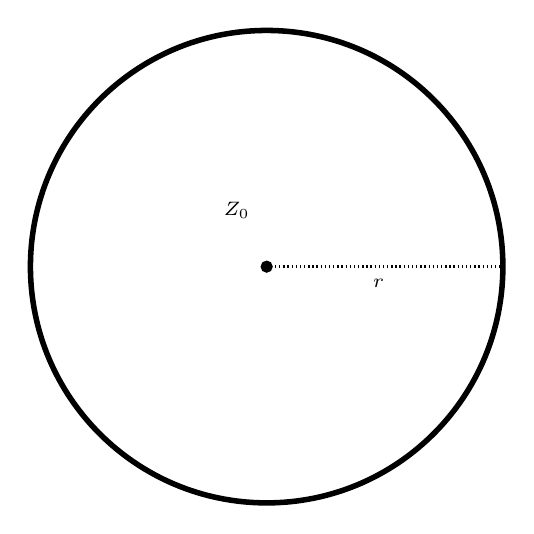
\begin{tikzpicture}
		\draw [line width=2pt] (0,0) circle (3cm);
		\draw [line width=1pt,dash pattern=on 0.5pt off 1pt] (0,0)-- (3,0);
		\begin{scriptsize}
			\draw [fill=black] (0,0) circle (2pt);
			\draw[color=black] (-0.38,0.71) node {$Z_0$};
			\draw[color=black] (1.42,-0.21) node {$r$};
		\end{scriptsize}
	\end{tikzpicture}
\end{center}
\begin{definition}
	The \textbf{\underline{modulus}} of $z = a+bi$ is $|z| = \sqrt{a^2+b^2}$

	The \underline{\textbf{distance}} between two numbers $z$ and $w$ is $|z-w|$
\end{definition}
Notes: \begin{itemize}
	\item $|z| \geq 0$ and is real
	\item $z\overline{z} = a^2+b^2 = |z|^2$
	\item $|z-z_0| = r$ describes a circule of radius $r$ centered at $z_0$
\end{itemize}
\begin{example}
	Sketch the sets: \begin{enumerate}
		\item $|z| < 3$
		\begin{center}
			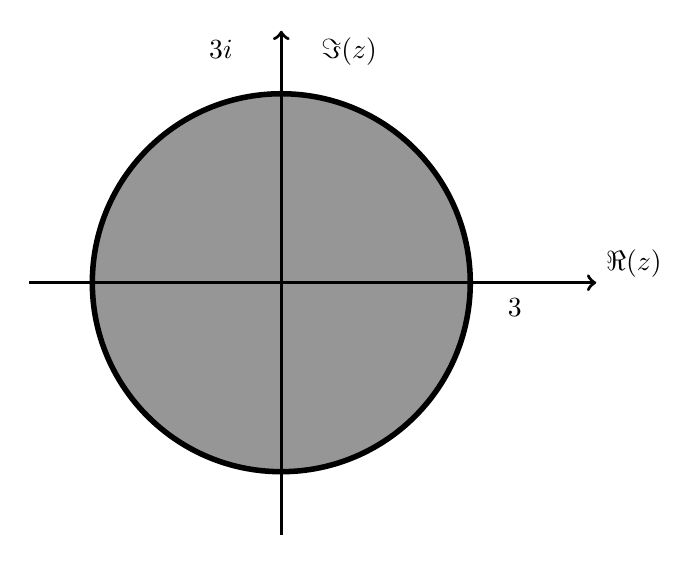
\begin{tikzpicture}[scale=0.8]
				\draw [line width=2pt,fill=black,fill opacity=0.41] (0,0) circle (3cm);
				\draw [->,line width=1.2pt] (0,-4) -- (0,4);
				\draw [->,line width=1.2pt] (-4,0) -- (5,0);
				\draw (-1.3,4) node[anchor=north west] {$3i$};
				\draw (3.44,-0.1) node[anchor=north west] {$3$};
				\draw (5,0.68) node[anchor=north west] {$\Re(z)$};
				\draw (0.48,4.04) node[anchor=north west] {$\Im(z)$};
			\end{tikzpicture}
		\end{center}
		\item $|z| = \Im(z)$. Let $z = a+ib$. So, $\sqrt{a^2+b^2} = b$, which gives $a^2+b^2 = b^2$, so $a = 0, b \geq 0$
		\begin{center}
			\begin{tikzpicture}[scale=0.8]
				\begin{axis}[
					x=1cm,y=1cm,
					axis lines=middle,
					xmin=-5,
					xmax=5,
					ymin=-1,
					ymax=5,
					xtick=\empty,
					ytick=\empty,]
				\end{axis}
				\draw [line width=3pt] (5,6)--(5,1);
				\draw (5.2,6) node[anchor=north west] {$\Im(z)$};
				\draw (10,1.5) node[anchor=north west] {$\Re (z)$};
			\end{tikzpicture}
		\end{center}
		\item $|z-1| = |z+i|$. So 
		\begin{align*}
		\sqrt{(a-1)^2+b^2} &= \sqrt{a^2+(b+1)^2} \\
		(a-1)^2+b^2 &= a^2+(b+1)^2\\
		a^2 - 2a+1+b^2 &= a^2+b^2+2b+1\\
		b &= -a
		\end{align*}
		This is the set of points that are equidistant from $z = 1$ and $z= -i$
		\begin{center}
			\begin{tikzpicture}[scale=0.8]
				\begin{axis}[
					x=1cm,y=1cm,
					axis lines=middle,
					xmin=-5,
					xmax=5,
					ymin=-5,
					ymax=5,
					xtick=\empty,
					ytick=\empty,]
				\end{axis}
			\draw [line width=2pt] (2,8)--(8,2);
			\draw (5.2,10) node[anchor=north west] {$\Im(z)$};
			\draw (10,5.5) node[anchor=north west] {$\Re(z)$};
			\end{tikzpicture}
		\end{center}
	\end{enumerate}
\end{example}

We will often use $z = x+yi$, so we are in the $xy$-plane, still not called $\mathbb{R}^2$ though. 

Useful inequalities: $$|z_1 + z_2| \leq |z_1| + |z_2|$$
This is known as ``Triangle Inequality''. This also extends to $$|z_1 = z_2 + \cdots + z_n| \leq |z_1| + \cdots + |z_n|$$

\begin{corollary}
	$$|z_1 + z_2| \geq \bigg||z_1| - |z_2|\bigg|$$
\end{corollary}
\begin{proof}
	\begin{align*}
		|z_1| &= |z_1 + (z_2-z_2)|\\
		&=|(z_1 + z_2)+(-z_2)|\\
		&\leq |z_1 + z_2| + |z_2|
	\end{align*}
	\begin{align*}
		|z_2| &= |z_2 + (z_1-z_1)|\\
		&=|(z_1 + z_2)+(-z_1)|\\
		&\leq |z_1 + z_2| + |z_1|
	\end{align*}
	So $|z_1+z_2| \geq |z_1| - |z_2|$ and $|z_2| - |z_1|$. So $$|z_1 + z_2| \geq \bigg||z_1| - |z_2|\bigg|$$
\end{proof}

\begin{definition}
	\textbf{\underline{Polar Form}}
	\begin{tcolorbox}[hbox, before=\par\smallskip\centering]
		$x = r\cos \theta$, $y = r\sin \theta$
	\end{tcolorbox}
	So, \begin{align*}
		z&= r\cos \theta + ir\sin\theta\\
		&=r(\cos \theta + i\sin\theta)\\
		&=r \underbrace{\cis}_{\text{common abreviation}} \theta
	\end{align*}
	\begin{tcolorbox}[hbox, before=\par\smallskip\centering]
		$r = \sqrt{x^2+y^2}$, $\tan \theta = \dfrac{y}{x}$
	\end{tcolorbox}
	\begin{center}
		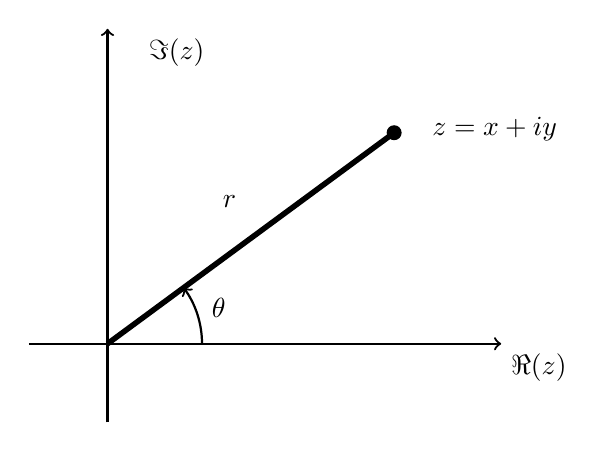
\begin{tikzpicture}
			\draw [->,line width=0.8pt] (-1,0) -- (5,0);
			\draw [->,line width=0.8pt] (0,-1) -- (0,4);
			\draw (0.4,4) node[anchor=north west] {$\Im(z)$};
			\draw (5,0) node[anchor=north west] {$\Re(z)$};
			\draw [line width=2pt] (0,0)-- (3.64,2.68);
			\draw [shift={(0,0)},->,line width=0.8pt] (0:1.2) arc (0:36.362868584929245:1.2);
			\draw (1.2,0.7) node[anchor=north west] {$\theta$};
			\draw (4,3) node[anchor=north west] {$z=x+iy$};
			\draw (1.34,2) node[anchor=north west] {$r$};
			\draw [fill=black] (3.64,2.68) circle (2.5pt);
			\end{tikzpicture}
	\end{center}
\end{definition}
Notes: \begin{itemize}
	\item This is not unique. e.g. $z = 2 = 2\cis 0 = 2\cis 2\pi = \cdots$, also $z = 0 = 0 \cis \theta$ for any $\theta$
	\item $\theta = \tan^{-1}(\dfrac{y}{x})[\pm 2k\pi]$ if $x > 0$, but must add $\pi$ if $x < 0$ - Recall principal values
\end{itemize}
\begin{example}
	Say we want to express $z = -1-i$ in polar form. 
	
	We compute $r = \sqrt{(-1)^2+(-1)^2} = \sqrt{2}$. $\tan \theta = \dfrac{-1}{-1} = 1$. Note that $\theta \neq \tan^{-1}(1) = \dfrac{\pi}{4}$, instead, $\theta = \dfrac{5\pi}{4}$. 

	So, $z = \sqrt{2}\cis \dfrac{5\pi}{4}$ or $\sqrt{2}\cis (\dfrac{5\pi}{4} + 2k\pi)$
	\begin{center}
		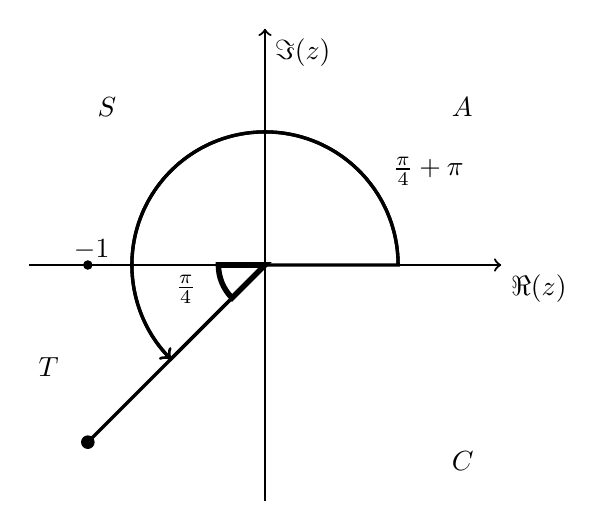
\begin{tikzpicture}[scale=1.5]
			\draw [->,line width=0.8pt] (-2,0) -- (2,0);
			\draw [->,line width=0.8pt] (0,-2) -- (0,2);
			\draw (0,2) node[anchor=north west] {$\Im(z)$};
			\draw (2,0) node[anchor=north west] {$\Re(z)$};
			\draw [fill=black] (-1.5,-1.5) circle (1.5pt);
			\draw [fill=black] (-1.5,0) circle (1pt);
			\draw (-1.7,0.3) node[anchor=north west] {$-1$};
			\draw [shift={(0,0)},line width=1.2pt] (0,0) -- (0:1.127026791712589) arc (0:225:1.127026791712589) -- cycle;
			\draw [shift={(0,0)},line width=2pt] (0,0) -- (180:0.39445937709940615) arc (180:225:0.39445937709940615) -- cycle;	
			\draw [line width=1.2pt] (0,0)-- (-1.5,-1.5);
			\draw [shift={(0,0)},->,line width=1.2pt] (0:1.127026791712589) arc (0:225:1.127026791712589);
			\draw (-0.84,0) node[anchor=north west] {$\frac{\pi}{4}$};
			\draw (1,1) node[anchor=north west] {$\frac{\pi}{4}+\pi$};
			\draw (1.5,1.5) node[anchor=north west] {$A$};
			\draw (-1.5,1.5) node[anchor=north west] {$S$};
			\draw (-2,-0.7) node[anchor=north west] {$T$};
			\draw (1.5,-1.5) node[anchor=north west] {$C$};
			\end{tikzpicture}
	\end{center}
\end{example}
Note: $$z = \underbrace{r}_{=\sqrt{x^2+y^2}, r = |z|, \text{``modulus''}}\cis \underbrace{\theta}_{\text{``argument'' of }z}$$
Also, ``$\arg z$'' = set of all possible values of $\theta$. ``$\Arg z$'' = principle values of $\theta$, usually in $(\pi, \pi]$

\begin{example}
	For $z = -1 + \sqrt{3}i$. $\Arg z = \dfrac{2\pi}{3}$, $\arg z = \dfrac{2\pi}{3} + 2k\pi, k \in \mathbb{Z}$

	Also, $|z| = 2$, so $-1 + \sqrt{3}i = 2\cis \dfrac{2\pi}{3}$
\end{example}

We sometimes think of $\arg z$ as a multivalued ``function'' of $z$. For a single-valued function, we could use $\Arg z$, but it has discontinuity on negative real axis. 
\begin{center}
	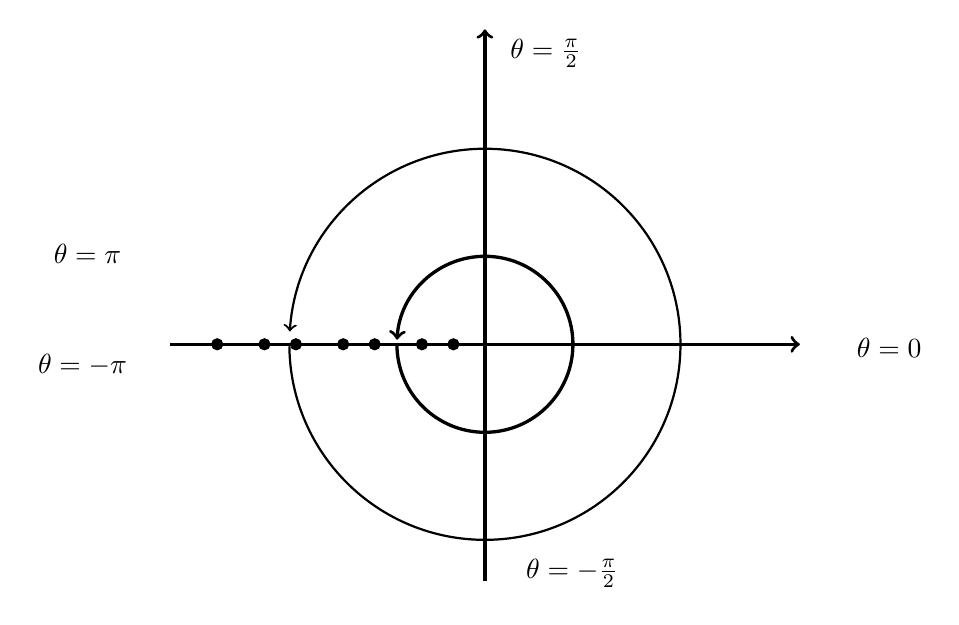
\begin{tikzpicture}[scale=2]
		\draw [->,line width=1.2pt] (0,-1.5) -- (0,2);
		\draw [->,line width=1.2pt] (-2,0) -- (2,0);
		
		\draw [shift={(0,0)},->,line width=1.2pt] (-180:0.558829190753239) arc (-180:177.02028294976014:0.558829190753239);
		\draw [shift={(0,0)},->,line width=0.8pt] (-179.42598203648794:1.241842646118309) arc (-179.42598203648794:176.2439591765568:1.241842646118309);
		\draw (2.3,0.1) node[anchor=north west] {$\theta=0$};
		\draw (0.1,2) node[anchor=north west] {$\theta=\frac{\pi}{2}$};
		\draw (0.2,-1.3) node[anchor=north west] {$\theta=-\frac{\pi}{2}$};
		\draw (-2.9,0) node[anchor=north west] {$\theta=-\pi$};
		\draw (-2.8,0.7) node[anchor=north west] {$\theta=\pi$};
		\begin{scriptsize}
			\draw [fill=black] (-0.2,0) circle (1pt);
			\draw [fill=black] (-0.4,0) circle (1pt);
			\draw [fill=black] (-0.7,0) circle (1pt);
			\draw [fill=black] (-0.9,0) circle (1pt);
			\draw [fill=black] (-1.2,0) circle (1pt);
			\draw [fill=black] (-1.4,0) circle (1pt);
			\draw [fill=black] (-1.7,0) circle (1pt);
		\end{scriptsize}
		\end{tikzpicture}
\end{center}

Another way: we can define $\Arg(z)$ to have range $[0, 2\pi)$. In general, $\Arg_{\theta_0}z$ has range $[\theta_0, \theta_0 + 2\pi)$, and usually we use $\Arg z = \Arg_{-\pi} z$
\begin{center}
	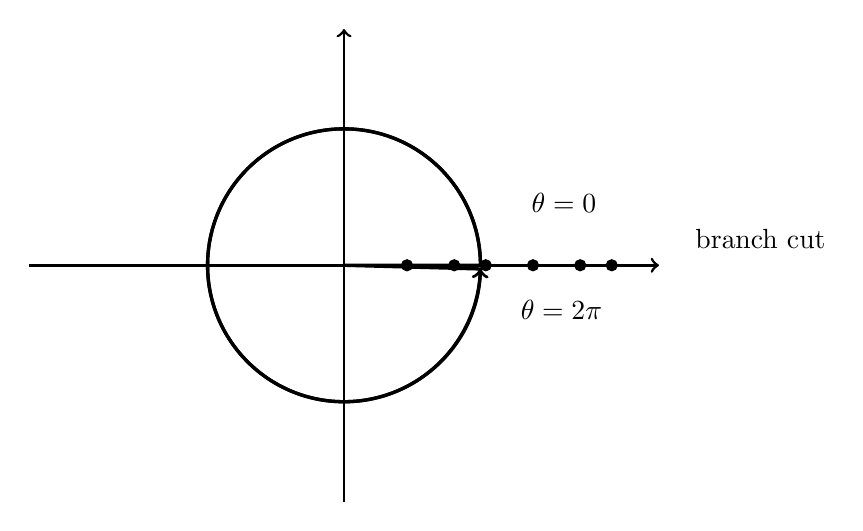
\begin{tikzpicture}[scale=2]
		\draw [shift={(0,0)},line width=1.2pt] (0,0) -- (0:0.8664438145013174) arc (0:358.45044092547164:0.8664438145013174) -- cycle;
		\draw [shift={(0,0)},->,line width=1.2pt] (0:0.8664438145013174) arc (0:358.45044092547164:0.8664438145013174);
		\draw (1.1296312880955108,0.5174728527862119) node[anchor=north west] {$\theta=0$};
		\draw [->,line width=1pt] (0,-1.5) -- (0,1.5);
		\draw [->,line width=1pt] (-2,0) -- (2,0);
		\draw (1.0603157829354055,-0.15835332252481515) node[anchor=north west] {$\theta=2\pi$};
		\draw (2.1693638654970915,0.2921974610158696) node[anchor=north west] {branch cut};
		\begin{scriptsize}
			\draw [fill=black] (0.4,0) circle (1pt);
			\draw [fill=black] (0.7,0) circle (1pt);
			\draw [fill=black] (0.9,0) circle (1pt);
			\draw [fill=black] (1.2,0) circle (1pt);
			\draw [fill=black] (1.5,0) circle (1pt);
			\draw [fill=black] (1.7,0) circle (1pt);
		\end{scriptsize}
	\end{tikzpicture}
\end{center}

\subsection{Complex Exponential, Powers and Roots}
Reading textbook Section 1.4, 1.5
\begin{definition}
	If $z = x+ iy$, then $e^z$ is defined to be the complex number $$e^z := e^x (\cos y + i\sin y)$$
\end{definition}
\begin{proposition}
	Euler's equation is formally consistent with the usual Taylor series expansions: \begin{align*}
		e^x &= 1 + x + \dfrac{x^2}{2!} + \dfrac{x^3}{3!} + \cdots\\
		\cos x &= 1 - \dfrac{x^2}{2!} + \dfrac{x^4}{4!} - \cdots\\
		\sin x &= x - \dfrac{x^3}{3!} + \dfrac{x^5}{5!} - \cdots
	\end{align*}
\end{proposition}
\begin{proof}
	Let's substitute $x = iy$ into the exponential series: \begin{align*}
		e^{iy} &= 1 + iy + \dfrac{(iy)^2}{2!} + \dfrac{(iy)^3}{3!} + \cdots\\
		&=(1-\dfrac{y^2}{2!} + \dfrac{y^4}{4!} - \cdots) + i(y-\dfrac{y^3}{3!} + \dfrac{y^5}{5!} - \cdots)\\
		&=\cos y + i\sin y
	\end{align*}
\end{proof}
As a result, we may introduce the standard polar representation $$z = r \cis \theta = r(\cos \theta + i \sin \theta) = re^{i\theta} = |z|e^{i \arg z}$$

Notice that $$e^{i0} = e^{2\pi i} = e^{-2\pi i} = e^{4\pi i} = e^{-4\pi i} = \cdots = 1$$
$$e^{(\pi / 2)i} = i \;\;\;\; e^{(-\pi/2) i}= -i \;\;\;\; e^{\pi i} = -1$$

Also notice that \begin{align*}
	\cos \theta &= \Re(e^{i\theta}) = \dfrac{e^{i\theta} + e^{-i\theta}}{2} \\
	\sin \theta &= \Im(e^{i\theta}) = \dfrac{e^{i\theta} - e^{-i\theta}}{2i} 
\end{align*}

Hence, $$z_1z_2 = (r_1e^{i\theta_1})(r_2e^{i\theta_2}) = (r_1r_2)e^{i(\theta_1+\theta_2)}$$
$$\dfrac{z_1}{z_2} = \dfrac{r_1e^{i\theta_1}}{r_2e^{i\theta_2}} = \dfrac{r_1}{r_2}e^{i(\theta_1-\theta_2)}$$
$$\overline{z} = re^{-i\theta}, \text{ given that }z = re^{i\theta}$$
\begin{example}
	Compute the following:
	\begin{enumerate}
		\item $(1+i)/(\sqrt{3}-i)$. 
		
		Notice that $1+i = \sqrt{2}\cis(\pi/4) = \sqrt{2}e^{i\pi/4}$, and $\sqrt{3}-i = 2\cis(-\pi /6) = 2e^{-i\pi/6}$. So, $$\dfrac{1+i}{\sqrt{3}-i} = \dfrac{\sqrt{2}e^{i\pi/4}}{2e^{-i\pi/6}} = \dfrac{\sqrt{2}}{2}e^{i5\pi/12}$$
		\item $(1+i)^{24}$
		
		We have $$(1+i)^{24} = (\sqrt{2}e^{i\pi/4})^{24} = (\sqrt{2})^{24}e^{i24\pi/4} = 2^{12}e^{i6\pi} = 2^{12}$$
	\end{enumerate}
\end{example}
\begin{theorem}
	$$(\cos \theta + i\sin \theta)^n = \cos n\theta + i \sin n\theta \;\;\;\; n = 1, 2, 3, ...$$
\end{theorem}
\begin{definition}
	There are exactly $m$ distinct $m$-th \underline{\textbf{roots of unity}}, denoted by $1^{1/m}$, and they are given by
	$$1^{1/m} = e^{i2k\pi/m} = \cos \dfrac{2k\pi}{m} + i\sin \dfrac{2k\pi}{m} \;\;\;\;(k = 0,1, 2, ..., m-1)$$

	Take $k = 1$ into the above equation, we can get $$\omega_m := e^{i2\pi/m} = \cos \dfrac{2\pi}{m} + i\sin \dfrac{2\pi}{m}$$
	So the complete set of roots can be displayed as$$\{1, \omega_m, \omega_m^2, \cdots, \omega_m^{m-1}\}$$
	Note that a number $w$ is said to be a \underline{\textbf{primitive}} $m$-th root of unity if $w^m = 1$ but $w^k \neq 1$ for $k = 1, 2, ..., m-1$. Clearly, $\omega_m$ is a primitive root. 
\end{definition}
\begin{theorem}
	$$1+\omega_m + \omega_m^2 + \cdots + \omega_m^{m-1} = 0$$
\end{theorem}
\begin{proof}
	Note that $$(\omega_m - 1) (1+\omega_m + \omega_m^2 + \cdots + \omega_m^{m-1}) = (\omega_m - 1) = 0$$
	Since $\omega_m \neq 1$, the result follows. 
\end{proof}
To obtain the $m$-th root of an arbitrary (non-zero) complex number $z = re^{i\theta}$, we can obtain the following generalized result. 
\begin{definition}
	The $m$-th distinct roots of $z$ are given by $$z^{1/m} = \sqrt[m]{|z|} e^{i (\theta + 2k\pi)/m}$$
\end{definition}
\begin{example}
	Find all the cube roots of $\sqrt{2} + i\sqrt{2}$

	The polar form for $\sqrt{2} + i\sqrt{2}$ is $$\sqrt{2} + i\sqrt{2} = 2e^{i\pi/4}$$
	Putting $|z|=2, \theta = \pi/4, m = 3$ into the above definition, we obtain $$(\sqrt{2} + i\sqrt{2})^{1/3} = \sqrt[3]{2}e^{i(\pi/12+2k\pi/3)}, \;\;\;\;(k = 0, 1, 2)$$
	Hence, the three cube roots of $\sqrt{2} + i\sqrt{2}$ are: \begin{itemize}
		\item $\sqrt[3]{2} (\cos \pi/12 + i\sin \pi/12)$
		\item $\sqrt[3]{2} (\cos 3\pi/4 + i\sin 3\pi/4)$
		\item $\sqrt[3]{2} (\cos 17\pi/12 + i\sin 17\pi/12)$
	\end{itemize}
\end{example}
\subsection{Application to Electrical Circuits}
A typical electrical circuits is like the following: 

\begin{center}
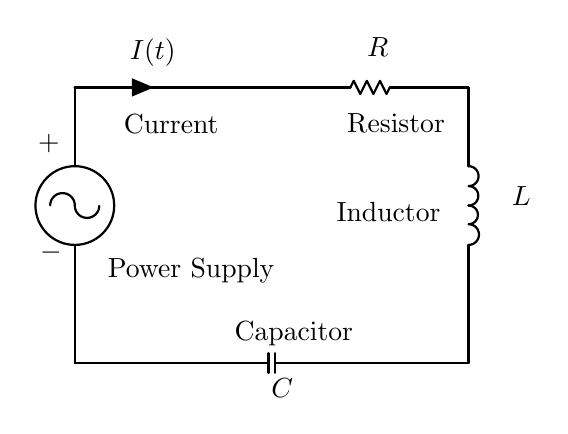
\begin{tikzpicture}[line cap=round,line join=round,>=triangle 45,x=1cm,y=1cm]
	\draw [line width=0.8pt] (0.5,-1.5)-- (-1.9583333333333333,-1.5);
	\draw [line width=0.8pt] (-4.5,-1.5)-- (-2.0416666666666665,-1.5);
	\draw [line width=0.8pt] (-1.9583333333333333,-1.625)-- (-1.9583333333333333,-1.375);
	\draw [line width=0.8pt] (-2.0416666666666665,-1.625)-- (-2.0416666666666665,-1.375);
	\draw [line width=0.8pt] (-0.5,2)-- (-0.5416666666666666,1.9166666666666667);
	\draw [line width=0.8pt] (-0.5416666666666666,1.9166666666666667)-- (-0.625,2.0833333333333335);
	\draw [line width=0.8pt] (-0.625,2.0833333333333335)-- (-0.7083333333333334,1.9166666666666667);
	\draw [line width=0.8pt] (-0.7083333333333334,1.9166666666666667)-- (-0.7916666666666666,2.0833333333333335);
	\draw [line width=0.8pt] (-0.7916666666666666,2.0833333333333335)-- (-0.875,1.9166666666666667);
	\draw [line width=0.8pt] (-0.875,1.9166666666666667)-- (-0.9583333333333334,2.0833333333333335);
	\draw [line width=0.8pt] (-0.9583333333333334,2.0833333333333335)-- (-1,2);
	\draw [line width=0.8pt] (0.5,2)-- (-0.5,2);
	\draw [line width=0.8pt] (-1,2)-- (-2,2);
	\draw [line width=0.8pt] (-4.5,2)-- (-2,2);
	\draw [line width=0.8pt] (-4.5,0.5) circle (0.5cm);
	\draw [line width=0.8pt] (-4.5,2)-- (-4.5,1);
	\draw [line width=0.8pt] (-4.5,0)-- (-4.5,-1.5);
	\draw [->,line width=0.8pt] (-4.5,2) -- (-3.5,2);
	\draw [shift={(-4.656590387120971,0.5012436450386237)},line width=0.8pt]  plot[domain=-0.007941859743208823:3.1336507938465843,variable=\t]({1*0.15659532557416184*cos(\t r)+0*0.15659532557416184*sin(\t r)},{0*0.15659532557416184*cos(\t r)+1*0.15659532557416184*sin(\t r)});
	\draw [shift={(-4.345017798262598,0.4979980972380158)},line width=0.8pt]  plot[domain=3.128676386995753:6.270269040585546,variable=\t]({1*0.15499513047202904*cos(\t r)+0*0.15499513047202904*sin(\t r)},{0*0.15499513047202904*cos(\t r)+1*0.15499513047202904*sin(\t r)});
	\draw (-1.1647903752888404,1.7891102514197603) node[anchor=north west] {Resistor};
	\draw (-1.3,0.6616607866585563) node[anchor=north west] {Inductor};
	\draw (-4.205103538689865,-0.04774561813501023) node[anchor=north west] {Power Supply};
	\draw (-2.5962711563901566,-0.8458278235277725) node[anchor=north west] {Capacitor};
	\draw (-4.002415994463131,1.7764422799055894) node[anchor=north west] {Current};
	\draw (-2.1275562103658316,-1.56790219983551) node[anchor=north west] {$C$};
	\draw (-3.926408165378105,2.7392081149825724) node[anchor=north west] {$I(t)$};
	\draw (-0.9114309450054217,2.7518760864967433) node[anchor=north west] {$R$};
	\draw (0.9254249245493644,0.8643483308852896) node[anchor=north west] {$L$};
	\draw (-5.091861544681832,1.5230828496221729) node[anchor=north west] {$+$};
	\draw (-5.066525601653489,0.14227395457755224) node[anchor=north west] {$-$};
	\draw [line width=0.8pt] (0.5,2)-- (0.5,1);
	\draw [line width=0.8pt] (0.5,0)-- (0.5,-1.5);
	\draw [shift={(0.5008148358603337,0.8734595181951952)},line width=0.8pt]  plot[domain=-1.564357086271925:1.577235567317868,variable=\t]({1*0.12654310527591534*cos(\t r)+0*0.12654310527591534*sin(\t r)},{0*0.12654310527591534*cos(\t r)+1*0.12654310527591534*sin(\t r)});
	\draw [shift={(0.5008148358603337,0.6234595181951952)},line width=0.8pt]  plot[domain=-1.5773962555897727:1.5641963980000206,variable=\t]({1*0.12346220713428468*cos(\t r)+0*0.12346220713428468*sin(\t r)},{0*0.12346220713428468*cos(\t r)+1*0.12346220713428468*sin(\t r)});
	\draw [shift={(0.5008148358603337,0.3817510753569967)},line width=0.8pt]  plot[domain=-1.5639055836783609:1.5776870699114327,variable=\t]({1*0.1182517320664097*cos(\t r)+0*0.1182517320664097*sin(\t r)},{0*0.1182517320664097*cos(\t r)+1*0.1182517320664097*sin(\t r)});
	\draw [shift={(0.5008148358603337,0.13175107535699673)},line width=0.8pt]  plot[domain=-1.5769809098747336:1.5646117437150597,variable=\t]({1*0.13175359507506548*cos(\t r)+0*0.13175359507506548*sin(\t r)},{0*0.13175359507506548*cos(\t r)+1*0.13175359507506548*sin(\t r)});
\end{tikzpicture}
\end{center}
Laws: \begin{enumerate}
	\item Resistor: $V = IR$
	\item Inductor: $V = L \dfrac{dI}{dt}$
	\item Capacitor: $C\dfrac{dV}{dt} = I$
\end{enumerate}
Suppose the current is $$I(t) = \underbrace{I_0}_{\text{amplitude}}\cos \underbrace{\omega}_{\text{frequency}} t = \Re(\underbrace{I_0e^{i\omega t}}_{\text{call it } \widetilde{I}(t)})$$
Then \begin{enumerate}
	\item Law 1 tells us $V = (I_0\cos \omega t)(R) = \Re(\widetilde{I}(t)\cdot R)$. So ``complex voltage'' is \begin{tcolorbox}[hbox, before=\par\smallskip\centering]
		$\tilde{V} = R\widetilde{I}$
	\end{tcolorbox}
	\item Law 2 tells us \begin{align*}
		V&= L\cdot (-\omega I_0\sin\omega t)\\
		&=-\omega LI_0\cdot \underbrace{\Re(e^{i(\omega t - \dfrac{\pi}{2})})}_{= \cos(\omega t - \dfrac{\pi}{2}) = \sin \omega t}\\
		&=\Re(-\omega L I_0 e^{i\omega t} e^{-i \dfrac{\pi}{2}})\\
		&=\Re(i\omega LI_0e^{i\omega t})
	\end{align*}
	So \begin{tcolorbox}[hbox, before=\par\smallskip\centering]
		$\widetilde{V} = i\omega L\widetilde{I}$
	\end{tcolorbox}
	\item Law 3 tells us \begin{align*}
		V &= \dfrac{1}{C}\int I(t)\\
		&= \dfrac{I_0}{C\omega} \sin \omega t\\
		&=\Re(\dfrac{I_0}{C\omega}e^{i(\omega t - \dfrac{\pi}{2})})\\
		&=\Re(\dfrac{I_0}{iC\omega}e^{i\omega t})
	\end{align*}
	So \begin{tcolorbox}[hbox, before=\par\smallskip\centering]
		$\widetilde{V} = \dfrac{1}{iC\omega}\widetilde{I}$
	\end{tcolorbox}
\end{enumerate}
So, with the complex representation, all three circuit elements behave like resistors with a complex ``Ohm's Law'
\begin{tcolorbox}[hbox, before=\par\smallskip\centering]
	$\widetilde{V} = Z\widetilde{I} \;\;\;\;\text{ where } Z = \begin{dcases}
		R & \text{for resistors}\\
		i\omega L & \text{for inductors}\\
		\dfrac{1}{i\omega C} & \text{for inductors}
	\end{dcases}$
\end{tcolorbox}
Moreover, $Z$ is called ``impedance''

Combining the components: \begin{itemize}
	\item In series: 
	\begin{center}
		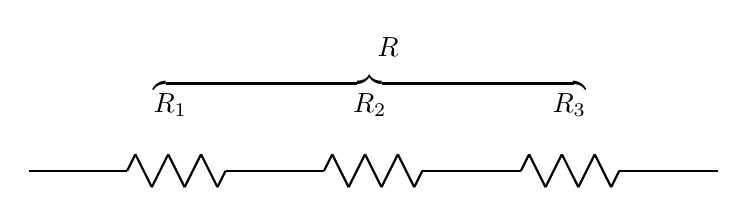
\begin{tikzpicture}[scale=2.5][line cap=round,line join=round,>=triangle 45,x=1cm,y=1cm]
			\draw (-0.4152701058878135,2.5331448905031593) node[anchor=north west] {$\overbrace{R_1\qquad\qquad\qquad R_2\qquad \qquad\qquad R_3}$};
			\draw (0.7212771477096162,2.723894079918112) node[anchor=north west] {$R$};
			\draw [line width=0.8pt] (0,2)-- (-0.04166666666666666,1.9166666666666667);
			\draw [line width=0.8pt] (-0.04166666666666666,1.9166666666666667)-- (-0.125,2.0833333333333335);
			\draw [line width=0.8pt] (-0.125,2.0833333333333335)-- (-0.20833333333333334,1.9166666666666667);
			\draw [line width=0.8pt] (-0.20833333333333334,1.9166666666666667)-- (-0.2916666666666667,2.0833333333333335);
			\draw [line width=0.8pt] (-0.2916666666666667,2.0833333333333335)-- (-0.375,1.9166666666666667);
			\draw [line width=0.8pt] (-0.375,1.9166666666666667)-- (-0.45833333333333337,2.0833333333333335);
			\draw [line width=0.8pt] (-0.45833333333333337,2.0833333333333335)-- (-0.5,2);
			\draw [line width=0.8pt] (0,2)-- (0,2);
			\draw [line width=0.8pt] (-0.5,2)-- (-0.5,2);
			\draw [line width=0.8pt] (0.5,2)-- (0.5416666666666666,2.0833333333333335);
			\draw [line width=0.8pt] (0.5416666666666666,2.0833333333333335)-- (0.625,1.9166666666666667);
			\draw [line width=0.8pt] (0.625,1.9166666666666667)-- (0.7083333333333334,2.0833333333333335);
			\draw [line width=0.8pt] (0.7083333333333334,2.0833333333333335)-- (0.7916666666666666,1.9166666666666667);
			\draw [line width=0.8pt] (0.7916666666666666,1.9166666666666667)-- (0.875,2.0833333333333335);
			\draw [line width=0.8pt] (0.875,2.0833333333333335)-- (0.9583333333333334,1.9166666666666667);
			\draw [line width=0.8pt] (0.9583333333333334,1.9166666666666667)-- (1,2);
			\draw [line width=0.8pt] (0.5,2)-- (0.5,2);
			\draw [line width=0.8pt] (1,2)-- (1,2);
			\draw [line width=0.8pt] (1.5,2)-- (1.5416666666666667,2.0833333333333335);
			\draw [line width=0.8pt] (1.5416666666666667,2.0833333333333335)-- (1.625,1.9166666666666667);
			\draw [line width=0.8pt] (1.625,1.9166666666666667)-- (1.7083333333333333,2.0833333333333335);
			\draw [line width=0.8pt] (1.7083333333333333,2.0833333333333335)-- (1.7916666666666667,1.9166666666666667);
			\draw [line width=0.8pt] (1.7916666666666667,1.9166666666666667)-- (1.875,2.0833333333333335);		\draw [line width=0.8pt] (1.875,2.0833333333333335)-- (1.9583333333333333,1.9166666666666667);
			\draw [line width=0.8pt] (1.9583333333333333,1.9166666666666667)-- (2,2);
			\draw [line width=0.8pt] (1.5,2)-- (1.5,2);
			\draw [line width=0.8pt] (2,2)-- (2,2);	
			\draw [line width=0.8pt] (0,2)-- (0.5,2);
			\draw [line width=0.8pt] (1,2)-- (1.5,2);
			\draw [line width=0.8pt] (2,2)-- (2.5,2);
			\draw [line width=0.8pt] (-0.5,2)-- (-1,2);
		\end{tikzpicture}
	\end{center}
	\begin{align*}
		R &= R_1 + R_2 + R_3 + \cdots\\
		L &= L_1 + L_2 + L_3 + \cdots\\
		\dfrac{1}{C} &= \dfrac{1}{C_1} + \dfrac{1}{C_2} + \dfrac{1}{C_3}+ \cdots\\
		Z &= Z_1 + Z_2+ Z_3 + \cdots
	\end{align*}
	\item In parallel: 
	\begin{center}
		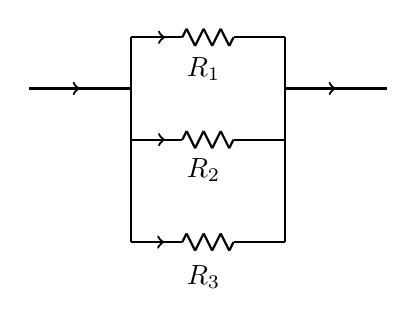
\begin{tikzpicture}[scale=1.3][line cap=round,line join=round,>=triangle 45,x=1cm,y=1cm]
			\draw (-2.55,0.9) node[anchor=north west] {$R_1$};
			\draw [line width=0.8pt] (-3,0.5)-- (-4,0.5);
			\draw [line width=0.8pt] (-1.5,0.5)-- (-0.5,0.5);
			\draw [line width=0.8pt] (-3,1)-- (-3,-1);
			\draw [line width=0.8pt] (-1.5,-1)-- (-1.5,1);
			\draw [line width=0.8pt] (-2.5,1)-- (-2.4583333333333335,1.0833333333333333);
			\draw [line width=0.8pt] (-2.4583333333333335,1.0833333333333333)-- (-2.375,0.9166666666666666);
			\draw [line width=0.8pt] (-2.375,0.9166666666666666)-- (-2.2916666666666665,1.0833333333333333);
			\draw [line width=0.8pt] (-2.2916666666666665,1.0833333333333333)-- (-2.2083333333333335,0.9166666666666666);
			\draw [line width=0.8pt] (-2.2083333333333335,0.9166666666666666)-- (-2.125,1.0833333333333333);
			\draw [line width=0.8pt] (-2.125,1.0833333333333333)-- (-2.0416666666666665,0.9166666666666666);
			\draw [line width=0.8pt] (-2.0416666666666665,0.9166666666666666)-- (-2,1);
			\draw [line width=0.8pt] (-3,1)-- (-2.5,1);
			\draw [line width=0.8pt] (-2,1)-- (-1.5,1);
			\draw [line width=0.8pt] (-2.5,0)-- (-2.4583333333333335,0.08333333333333333);
			\draw [line width=0.8pt] (-2.4583333333333335,0.08333333333333333)-- (-2.375,-0.08333333333333333);
			\draw [line width=0.8pt] (-2.375,-0.08333333333333333)-- (-2.2916666666666665,0.08333333333333333);
			\draw [line width=0.8pt] (-2.2916666666666665,0.08333333333333333)-- (-2.2083333333333335,-0.08333333333333333);
			\draw [line width=0.8pt] (-2.2083333333333335,-0.08333333333333333)-- (-2.125,0.08333333333333333);
			\draw [line width=0.8pt] (-2.125,0.08333333333333333)-- (-2.0416666666666665,-0.08333333333333333);
			\draw [line width=0.8pt] (-2.0416666666666665,-0.08333333333333333)-- (-2,0);
			\draw [line width=0.8pt] (-3,0)-- (-2.5,0);
			\draw [line width=0.8pt] (-2,0)-- (-1.5,0);
			\draw [line width=0.8pt] (-2.5,-1)-- (-2.4583333333333335,-0.9166666666666666);
			\draw [line width=0.8pt] (-2.4583333333333335,-0.9166666666666666)-- (-2.375,-1.0833333333333333);
			\draw [line width=0.8pt] (-2.375,-1.0833333333333333)-- (-2.2916666666666665,-0.9166666666666666);
			\draw [line width=0.8pt] (-2.2916666666666665,-0.9166666666666666)-- (-2.2083333333333335,-1.0833333333333333);
			\draw [line width=0.8pt] (-2.2083333333333335,-1.0833333333333333)-- (-2.125,-0.9166666666666666);
			\draw [line width=0.8pt] (-2.125,-0.9166666666666666)-- (-2.0416666666666665,-1.0833333333333333);
			\draw [line width=0.8pt] (-2.0416666666666665,-1.0833333333333333)-- (-2,-1);
			\draw [line width=0.8pt] (-3,-1)-- (-2.5,-1);
			\draw [line width=0.8pt] (-2,-1)-- (-1.5,-1);
			\draw [->,line width=0.8pt] (-4,0.5) -- (-3.5,0.5);
			\draw [->,line width=0.8pt] (-1.5,0.5) -- (-1,0.5);
			\draw (-2.55,-0.09) node[anchor=north west] {$R_2$};
			\draw (-2.55,-1.13) node[anchor=north west] {$R_3$};
			\draw [->,line width=0.8pt] (-3,1) -- (-2.666666666666666,1);
			\draw [->,line width=0.8pt] (-3,0) -- (-2.666666666666666,0);
			\draw [->,line width=0.8pt] (-3,-1) -- (-2.675555555555555,-1);
		\end{tikzpicture}
	\end{center}
	\begin{align*}
		\dfrac{1}{R} &= \dfrac{1}{R_1} + \dfrac{1}{R_2} +\dfrac{1}{R_3} + \cdots\\
		\dfrac{1}{L} &= \dfrac{1}{L_1} + \dfrac{1}{L_2} +\dfrac{1}{L_3} + \cdots\\
		C &= C_1 + C_2 + C_3 + \cdots\\
		\dfrac{1}{Z} &= \dfrac{1}{Z_1} + \dfrac{1}{Z_2} +\dfrac{1}{Z_3} + \cdots
	\end{align*}
\end{itemize}
\begin{example}
	Suppose a current $I(t) = I_0 \cos t$, passes through this: 

	\begin{center}
		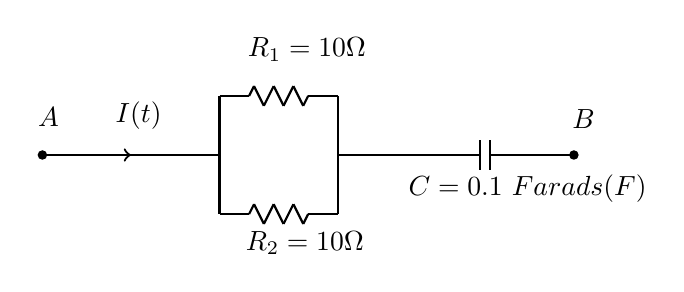
\begin{tikzpicture}[scale=1.5][line cap=round,line join=round,>=triangle 45,x=1cm,y=1cm]
			\draw (-1.36,-0.062222222222223025) node[anchor=north west] {$R_2=10\Omega$};
			\draw (-1.3422222222222224,1.573333333333327) node[anchor=north west] {$R_1=10\Omega$};
			\draw [line width=0.8pt] (-1.25,0)-- (-1.2083333333333333,0.08333333333333333);
			\draw [line width=0.8pt] (-1.2083333333333333,0.08333333333333333)-- (-1.125,-0.08333333333333333);
			\draw [line width=0.8pt] (-1.125,-0.08333333333333333)-- (-1.0416666666666667,0.08333333333333333);
			\draw [line width=0.8pt] (-1.0416666666666667,0.08333333333333333)-- (-0.9583333333333334,-0.08333333333333333);
			\draw [line width=0.8pt] (-0.9583333333333334,-0.08333333333333333)-- (-0.875,0.08333333333333333);
			\draw [line width=0.8pt] (-0.875,0.08333333333333333)-- (-0.7916666666666666,-0.08333333333333333);
			\draw [line width=0.8pt] (-0.7916666666666666,-0.08333333333333333)-- (-0.75,0);
			\draw [line width=0.8pt] (-1.5,0)-- (-1.25,0);
			\draw [line width=0.8pt] (-0.75,0)-- (-0.5,0);
			\draw [line width=0.8pt] (-1.25,1)-- (-1.2083333333333333,1.0833333333333333);
			\draw [line width=0.8pt] (-1.2083333333333333,1.0833333333333333)-- (-1.125,0.9166666666666666);
			\draw [line width=0.8pt] (-1.125,0.9166666666666666)-- (-1.0416666666666667,1.0833333333333333);
			\draw [line width=0.8pt] (-1.0416666666666667,1.0833333333333333)-- (-0.9583333333333334,0.9166666666666666);
			\draw [line width=0.8pt] (-0.9583333333333334,0.9166666666666666)-- (-0.875,1.0833333333333333);
			\draw [line width=0.8pt] (-0.875,1.0833333333333333)-- (-0.7916666666666666,0.9166666666666666);
			\draw [line width=0.8pt] (-0.7916666666666666,0.9166666666666666)-- (-0.75,1);
			\draw [line width=0.8pt] (-1.5,1)-- (-1.25,1);
			\draw [line width=0.8pt] (-0.75,1)-- (-0.5,1);
			\draw [line width=0.8pt] (-1.5,1)-- (-1.5,0);
			\draw [line width=0.8pt] (-0.5,1)-- (-0.5,0);
			\draw [line width=0.8pt] (-0.5,0.5)-- (0.5,0.5);
			\draw [line width=0.8pt] (-1.5,0.5)-- (-3,0.5);
			\draw [->,line width=0.8pt] (-3,0.5) -- (-2.25,0.5);
			\draw [line width=0.8pt] (0.5,0.5)-- (0.7083333333333334,0.5);
			\draw [line width=0.8pt] (1,0.5)-- (0.7916666666666666,0.5);
			\draw [line width=0.8pt] (0.7083333333333334,0.625)-- (0.7083333333333334,0.375);
			\draw [line width=0.8pt] (0.7916666666666666,0.625)-- (0.7916666666666666,0.375);
			\draw [line width=0.8pt] (1,0.5)-- (1.5,0.5);
			\draw (-2.4622222222222225,1.0311111111111066) node[anchor=north west] {$I(t)$};
			\draw (-3.12,0.9866666666666624) node[anchor=north west] {$A$};
			\draw (1.4044444444444446,0.9688888888888847) node[anchor=north west] {$B$};
			\draw (0.01777777777777778,0.41777777777777536) node[anchor=north west] {$C=0.1 \ Farads(F)$};
			\begin{scriptsize}
				\draw [fill=black] (-3,0.5) circle (1pt);
				\draw [fill=black] (1.5,0.5) circle (1pt);
			\end{scriptsize}
		\end{tikzpicture}
	\end{center}
	
	Find $V(t)$, the difference in electrical potential energy between $A$ and $B$
	
	\underline{\textbf{Solution}}: 
	
	\begin{center}
		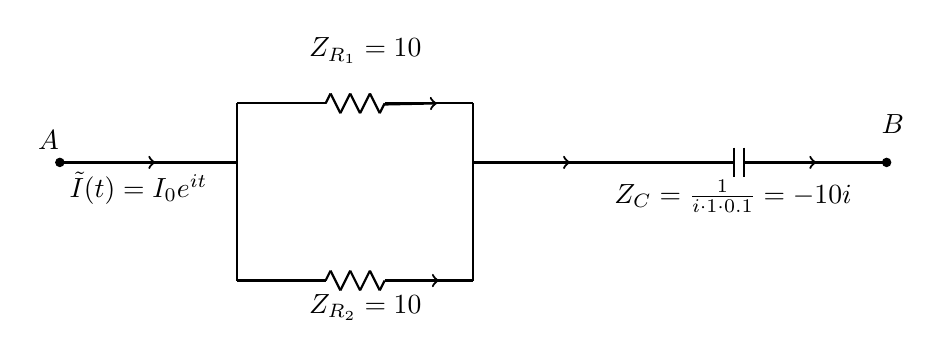
\begin{tikzpicture}[scale=1.5][line cap=round,line join=round,>=triangle 45,x=1cm,y=1cm]
			\draw (-2.4727988094140407,1.6361413165955456) node[anchor=north west] {$Z_{R_1}=10$};
			\draw [line width=0.8pt] (-2.25,-0.5)-- (-2.2083333333333335,-0.4166666666666667);
			\draw [line width=0.8pt] (-2.2083333333333335,-0.4166666666666667)-- (-2.125,-0.5833333333333334);
			\draw [line width=0.8pt] (-2.125,-0.5833333333333334)-- (-2.0416666666666665,-0.4166666666666667);
			\draw [line width=0.8pt] (-2.0416666666666665,-0.4166666666666667)-- (-1.9583333333333333,-0.5833333333333334);
			\draw [line width=0.8pt] (-1.9583333333333333,-0.5833333333333334)-- (-1.875,-0.4166666666666667);
			\draw [line width=0.8pt] (-1.875,-0.4166666666666667)-- (-1.7916666666666667,-0.5833333333333334);
			\draw [line width=0.8pt] (-1.7916666666666667,-0.5833333333333334)-- (-1.75,-0.5);
			\draw [line width=0.8pt] (-3,-0.5)-- (-2.25,-0.5);
			\draw [line width=0.8pt] (-1.75,-0.5)-- (-1,-0.5);
			\draw [line width=0.8pt] (-2.25,1)-- (-2.2083333333333335,1.0833333333333333);
			\draw [line width=0.8pt] (-2.2083333333333335,1.0833333333333333)-- (-2.125,0.9166666666666666);
			\draw [line width=0.8pt] (-2.125,0.9166666666666666)-- (-2.0416666666666665,1.0833333333333333);
			\draw [line width=0.8pt] (-2.0416666666666665,1.0833333333333333)-- (-1.9583333333333333,0.9166666666666666);
			\draw [line width=0.8pt] (-1.9583333333333333,0.9166666666666666)-- (-1.875,1.0833333333333333);
			\draw [line width=0.8pt] (-1.875,1.0833333333333333)-- (-1.7916666666666667,0.9166666666666666);
			\draw [line width=0.8pt] (-1.7916666666666667,0.9166666666666666)-- (-1.75,1);
			\draw [line width=0.8pt] (-3,1)-- (-2.25,1);
			\draw [line width=0.8pt] (-1.75,1)-- (-1,1);
			\draw [line width=0.8pt] (1,0.5)-- (1.2083333333333333,0.5);
			\draw [line width=0.8pt] (1.5,0.5)-- (1.2916666666666667,0.5);
			\draw [line width=0.8pt] (1.2083333333333333,0.625)-- (1.2083333333333333,0.375);
			\draw [line width=0.8pt] (1.2916666666666667,0.625)-- (1.2916666666666667,0.375);
			\draw [line width=0.8pt] (1.5,0.5)-- (2.5,0.5);
			\draw (-4.5,0.5) node[anchor=north west] {$\tilde{I}(t)=I_0e^{it}$};
			\draw (-4.7678511966796515,0.8504477065406559) node[anchor=north west] {$A$};
			\draw (2.375757810529975,0.9848426661553081) node[anchor=north west] {$B$};
			\draw (0.11171964471389924,0.43692475388018776) node[anchor=north west] {$Z_C=\frac{1}{i\cdot1\cdot0.1}=-10i$};
			\draw [line width=0.8pt] (-1,1)-- (-1,0.5);
			\draw [line width=0.8pt] (-1,0.5)-- (-1,-0.5);
			\draw [line width=0.8pt] (-3,1)-- (-3,0.5);
			\draw [line width=0.8pt] (-3,0.5)-- (-3,-0.5);
			\draw [line width=0.8pt] (-4.5,0.5)-- (-3,0.5);
			\draw [line width=0.8pt] (-1,0.5)-- (1,0.5);
			\draw [->,line width=0.8pt] (-4.5,0.5) -- (-3.6898720450852003,0.5);
			\draw [->,line width=0.8pt] (-1.7547447843933128,0.9905104312133761) -- (-1.306134363426703,1);
			\draw [->,line width=0.8pt] (-1.7418713589986865,-0.5) -- (-1.2890466381101549,-0.5);
			\draw [->,line width=0.8pt] (-1,0.5) -- (-0.178344492534511,0.5);
			\draw [->,line width=0.8pt] (1.5,0.5) -- (1.9063579960843895,0.5);
			\draw (-2.4727988094140407,-0.5348541848719125) node[anchor=north west] {$Z_{R_2}=10$};
			\begin{scriptsize}
				\draw [fill=black] (-4.5,0.5) circle (1pt);
				\draw [fill=black] (2.5,0.5) circle (1pt);
			\end{scriptsize}
		\end{tikzpicture}
	\end{center}

	Let's use the complex version of ``Ohm's Law''. We have $\dfrac{1}{Z_R} = \dfrac{1}{Z_{R_1}} + \dfrac{1}{Z_{R_2}} = \dfrac{1}{10} + \dfrac{1}{10} = \dfrac{1}{5}$, so $Z_R = 5$. 

	Combine the resistor and capacitor in series: $Z = Z_R + Z_C = 5-10i$. 

	So, the complex voltage is \begin{align*}
		\widetilde{V} &= Z \widetilde{I}\\
		&= (5-10i)I_0e^{it}\\
		&=5I_0(1-2i)e^{it}\\
		&=5I_0\sqrt{5}e^{i\arctan -2} e^{it}
	\end{align*}
	So, $V(t) = \Re(\widetilde{V}(t)) \approx 5\sqrt{5} I_0 \cos(t-1.107)$
	\begin{center}
		\begin{tikzpicture}[scale=1.5][line cap=round,line join=round,>=triangle 45,x=1cm,y=1cm]
			\begin{axis}[
				x=1cm,y=1cm,
				axis lines=middle,
				xmin=-1.9140740740740745,
				xmax=3.3718518518518503,
				ymin=-2.1896296296296267,
				ymax=0.583703703703702,
				xtick={0,1},
				ytick={-2,-1,...,0},]
				\draw [->,line width=0.8pt] (0,0) -- (1,-2);	
				\draw (0.38,-0.4) node[anchor=north west] {$\arctan2$};
				\end{axis}
			\draw [shift={(1.5,1.75)},<-,line width=1pt] (-2:0.65) arc (-63.43494882292201:0:0.5333333333333332);
		\end{tikzpicture}
	\end{center}
\end{example}

\subsection{Sets in the Complex Plane}
\begin{definition}
	\textbf{\underline{Neighborhood of $z_0$}} is $$N_\epsilon(z_0) = \{z \in \mathbb{C} : |z-z_0| < \epsilon\}$$ where $\epsilon > 0$ is real
\end{definition}
\begin{definition}
	\textbf{\underline{Deleted Neighborhood of $z_0$}} is $$DN_\epsilon(z_0) = \{z \in \mathbb{C} : 0 < |z-z_0| < \epsilon\}$$ where $\epsilon > 0$ is real
\end{definition}
\begin{example}
	For $z_0 = 1+i$, consider $|z-(1+i)| < 1$. The neighborhood of $z_0$ and deleted neighborhood of $z_0$ is as follows: 

	\begin{center}
		\definecolor{uu}{rgb}{0.3,0.3,0.3}
		\begin{tikzpicture}[line cap=round,line join=round,>=triangle 45,x=1cm,y=1cm]
			\draw[->] (-1,0)--(5,0);
			\draw[->] (0,-1)--(0,5);
			\draw [dashed,line width=1.2pt,fill=black,fill opacity=0.27] (2,2) circle (2cm);
			\draw (2.05,3.2) node[anchor=north west] {$N_1(1+i)$};
			\draw [fill=black] (2,2) circle (1.5pt);
			\draw [fill=uu] (0,2) circle (1pt);
			\draw[color=uu] (-0.25,2.) node {i};
			\draw [fill=black] (0,4) circle (1pt);
			\draw[color=black] (-0.25,4) node {2i};
			\draw [fill=uu] (2,0) circle (2pt);
			\draw[color=uu] (2,-0.35) node {1};
			\draw [fill=black] (4,0) circle (1pt);
			\draw[color=black] (4,-0.35) node {2};
		\end{tikzpicture}
		\begin{tikzpicture}[line cap=round,line join=round,>=triangle 45,x=1cm,y=1cm]
			\draw[->] (-1,0)--(5,0);
			\draw[->] (0,-1)--(0,5);
			\draw [dashed,line width=1.2pt,fill=black,fill opacity=0.27] (2,2) circle (2cm);
			\draw (1.7,3.1) node[anchor=north west] {$DN_1(1+i)$};
			\draw [color=black] (2,2) circle (1.5pt);
			\draw [fill=uu] (0,2) circle (1pt);
			\draw[color=uu] (-0.25,2.) node {i};
			\draw [fill=black] (0,4) circle (1pt);
			\draw[color=black] (-0.25,4) node {2i};
			\draw [fill=uu] (2,0) circle (2pt);
			\draw[color=uu] (2,-0.35) node {1};
			\draw [fill=black] (4,0) circle (1pt);
			\draw[color=black] (4,-0.35) node {2};
		\end{tikzpicture}
	\end{center}
\end{example}
\begin{definition}
	Let $S \subseteq \mathbb{C}$: \begin{itemize}
		\item $z_0$ is an \underline{\textbf{interior point}} of $S$ if there exists a neighborhood of $z_0$ which contains only points in $S$
		\item $z_0$ is an \underline{\textbf{exterior point}} of $S$ if there exists a neighborhood of $z_0$ which contains no points in $S$
		\item $z_0$ is a \underline{\textbf{boundary point}} of $S$ if every neighborhood of $z_0$ contains some points in $S$ and some points not. 
		\item \underline{\textbf{Boundary of $S$}} is the set of all boundary points of $S$
		\item $S$ is \underline{\textbf{open}} if it contains none of its boundary points
		\item $S$ is \underline{\textbf{closed}} if it contains all of its boundary points, equivalently if its complement is open. 
		\item Note that $S$ could be both open and closed, when it does not have any boundary points
	\end{itemize}
	\begin{center}
		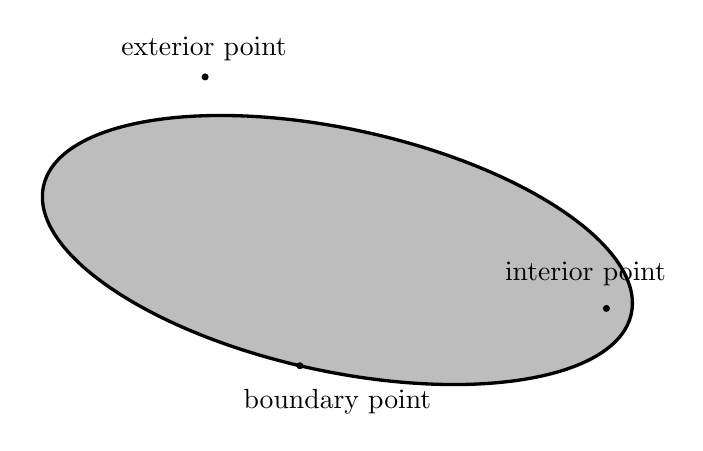
\begin{tikzpicture}[scale=0.7][line cap=round,line join=round,>=triangle 45,x=1cm,y=1cm]
			\draw [rotate around={-12.2550245737389:(0.82,-1.26)},line width=1.2pt,fill=black,fill opacity=0.26] (0.82,-1.26) ellipse (5.456218028894557cm and 2.1982527559027356cm);
			\draw [fill=black] (5.7,-2.32) circle (1.5pt);
			\draw[color=black] (5.32,-1.69) node {interior point};
			\draw [fill=black] (0.14,-3.36) circle (1.5pt);
			\draw[color=black] (0.82,-4.01) node {boundary point};
			\draw [fill=black] (-1.58,1.88) circle (1.5pt);
			\draw[color=black] (-1.6,2.39) node {exterior point};
		\end{tikzpicture}
	\end{center}
\end{definition}
\begin{example}
	Note that \begin{itemize}
		\item $N_1(1+i)$ is open
		\item $\mathbb{C}$ is both open and closed
		\item $|z-z_0| \leq 1$ is closed
		\item The figure below: it is neither open nor closed. 
		\begin{center}
			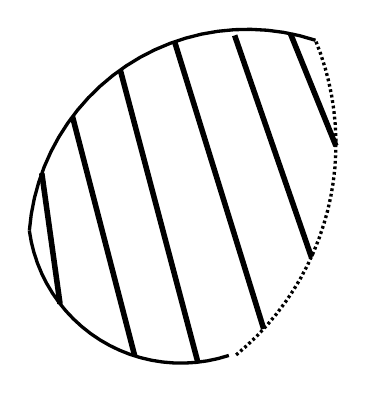
\begin{tikzpicture}[scale=1][line cap=round,line join=round,>=triangle 45,x=1cm,y=1cm]
				\draw [shift={(-2.2,-0.04)},line width=1.2pt,dash pattern=on 1pt off 1pt]  plot[domain=-0.8834434406912877:0.38931672183314087,variable=\t]({1*3.467333269243094*cos(\t r)+0*3.467333269243094*sin(\t r)},{0*3.467333269243094*cos(\t r)+1*3.467333269243094*sin(\t r)});
				\draw [shift={(0.14,-1.36)},line width=1.2pt]  plot[domain=1.2527427180455013:3.0628086926006493,variable=\t]({1*2.7752379743583204*cos(\t r)+0*2.7752379743583204*sin(\t r)},{0*2.7752379743583204*cos(\t r)+1*2.7752379743583204*sin(\t r)});
				\draw [shift={(-0.7,-0.88)},line width=1.2pt]  plot[domain=3.2765392412560086:5.030186986194582,variable=\t]({1*1.944306222620606*cos(\t r)+0*1.944306222620606*sin(\t r)},{0*1.944306222620606*cos(\t r)+1*1.944306222620606*sin(\t r)});
				\draw [line width=2pt] (-2.4682557768735838,-0.41187151887202067)-- (-2.2364548804155135,-2.071483565882702);
				\draw [line width=2pt] (-2.078453794925833,0.3074557187822542)-- (-1.2880175887067855,-2.733257133452524);
				\draw [line width=2pt] (-1.471600098553103,0.8993563102494704)-- (-0.4865924018176054,-2.8125588954438703);
				\draw [line width=2pt] (-0.7815545996879623,1.2577629636990497)-- (0.34969242697916547,-2.3897805275823303);
				\draw [line width=2pt] (-0.01921974959665283,1.3379878398032463)-- (0.9554416977355595,-1.4772152560391683);
				\draw [line width=2pt] (0.6895144756631459,1.3602903623247886)-- (1.2672454540513378,-0.06467714246696885);
			\end{tikzpicture}
		\end{center}
	\end{itemize}
\end{example}
\begin{definition}
	For $S \subseteq \mathbb{C}$: \begin{itemize}
		\item \underline{\textbf{Closure}} of $S$ is $S$ plus its boundary.
		\item An open set $S$ is \underline{\textbf{connected}} if any two points in $S$ can be connected by a polygonal path lying entirely in $S$
		\item A \underline{\textbf{domain}} is an open connected set. We should not confuse this with ``domain of a function''
		\item A \underline{\textbf{region}} is a domain plus some, none, or all of its boundary points. 
		\item $S$ is \underline{\textbf{bounded}} if there exists $R \in \mathbb{R}$ such that $|z| < R$ for all $z \in S$
	\end{itemize}
	\begin{center}
		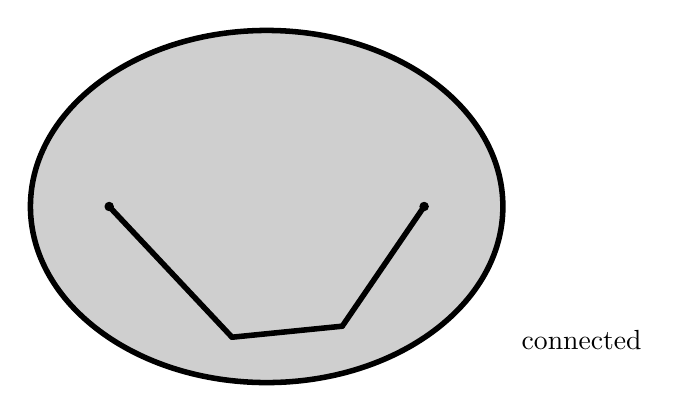
\begin{tikzpicture}[line cap=round,line join=round,>=triangle 45,x=1cm,y=1cm]
			\draw [rotate around={0:(0,0)},line width=2pt,fill=black,fill opacity=0.19] (0,0) ellipse (3cm and 2.23606797749979cm);
			\draw [line width=2pt] (-2,0)-- (-0.44,-1.66);
			\draw [line width=2pt] (-0.44,-1.66)-- (0.96,-1.52);
			\draw [line width=2pt] (0.96,-1.52)-- (2,0);
			\begin{scriptsize}
				\draw [fill=black] (-2,0) circle (1.5pt);
				\draw [fill=black] (2,0) circle (1.5pt);
			\end{scriptsize}
			\draw[color=black] (4,-1.69) node {connected};
		\end{tikzpicture}
		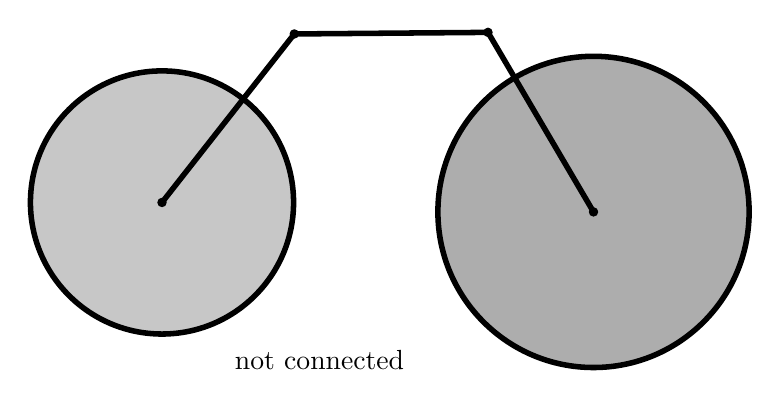
\begin{tikzpicture}[line cap=round,line join=round,>=triangle 45,x=1cm,y=1cm]
			\draw [line width=2pt,fill=black,fill opacity=0.22] (-2,0) circle (1.6709278859364338cm);
			\draw [line width=2pt,fill=black,fill opacity=0.32] (3.48,-0.12) circle (1.9762590923257002cm);
			\draw [line width=2pt] (-2,0)-- (-0.32,2.14);
			\draw [line width=2pt] (-0.32,2.14)-- (2.14,2.16);
			\draw [line width=2pt] (2.14,2.16)-- (3.48,-0.12);
			\begin{scriptsize}
				\draw [fill=black] (-2,0) circle (1.5pt);
				\draw [fill=black] (-0.32,2.14) circle (1.5pt);
				\draw [fill=black] (2.14,2.16) circle (1.5pt);
				\draw [fill=black] (3.48,-0.12) circle (1.5pt);		
			\end{scriptsize}
			\draw[color=black] (0,-2) node {not connected};
		\end{tikzpicture}
	\end{center}
\end{definition}
\begin{theorem}
	If $u(x, y)$, defined on a domain $D$, satisfies $$\dfrac{\partial u}{\partial x} = \dfrac{\partial u}{\partial y} = 0$$ for all points in $D$, then $u(x, y) = $ constant in $D$. 
\end{theorem}
\begin{example}
	Suppose we have $S_1$ and $S_2$ like this: 
	\begin{center}
		\begin{tikzpicture}[line cap=round,line join=round,>=triangle 45,x=1cm,y=1cm]
			\draw[->] (-5,0)--(5,0);
			\draw[->] (0,-1)--(0,4);
			\draw [rotate around={-0.83:(-2.77,1.55)},line width=0.5pt,
			dash pattern=on 1pt off 1pt] (-2.77,1.55) ellipse (1.19cm and 0.97cm);
			\draw [rotate around={-4.1:(2.52,1.56)},line width=0.5,
			dash pattern=on 1pt off 1pt] (2.52,1.56) ellipse (1.35cm and 1.22cm);
			\draw[color=black] (-2.9,1.77) node {$S_1$};
			\draw[color=black] (2.56,1.89) node {$S_2$};
		\end{tikzpicture}
	\end{center}
	
	in which we have $u(x,y) = 0$ on $S_1$ and $u(x,y) = 1$ on $S_2$. 

	Then, $\dfrac{\partial u}{\partial x} = \dfrac{\partial u}{\partial y} = 0$ on $S_1 \cup S_2$, but $u(x,y)$ is not constant on $S_1 \cup S_2$.

	Why does not the theorem hold? Well this is because $S_1 \cup S_2$ is not connected, so it's not a domain. 
\end{example}
The Extended Complex Plane: 

The ``neighborhood of $\infty$'' is defined as: $$N_\epsilon(\infty) = \{z \in \mathbb{C} : |z| > \dfrac{1}{\epsilon}\}$$ for some real $\epsilon > 0$
The Riemann sphere: 

\begin{center}
	\definecolor{zzttqq}{rgb}{0.6,0.2,0}
	\begin{tikzpicture}[scale=0.8][line cap=round,line join=round,>=triangle 45,x=1cm,y=1cm]
		\fill[line width=2pt,color=zzttqq,fill=zzttqq,fill opacity=0.10000000149011612] (-4,2) -- (-8,-2) -- (5,-2) -- (9,2) -- cycle;
		\draw [->,line width=2pt] (0,-4.801835999999982) -- (0,5.06);
		\draw [->,line width=2pt] (-5,0) -- (6,0);
		\draw [->,line width=2pt] (3.5,3.5) -- (-4,-4);
		\draw [shift={(0,0)},line width=1pt]  plot[domain=0:3.141592653589793,variable=\t]({1*4*cos(\t r)+0*4*sin(\t r)},{0*4*cos(\t r)+1*4*sin(\t r)});
		\draw [shift={(0,0)},line width=1pt,dash pattern=on 1pt off 1pt]  plot[domain=3.141592653589793:6.283185307179586,variable=\t]({1*4*cos(\t r)+0*4*sin(\t r)},{0*4*cos(\t r)+1*4*sin(\t r)});
		\draw [rotate around={0:(-0.01,0)},line width=1.2pt,dash pattern=on 1pt off 1pt] (-0.01,0) ellipse (3.998253390825929cm and 1.4398368578596104cm);
		\draw [line width=1pt,dash pattern=on 1pt off 1pt] (0,4)-- (5,-1);
		\draw (-10,4.68) node[anchor=north west] {Riemann Sphere $x_1^2+x_2^2+x_3^2=1$};
		\draw [->,line width=1pt] (-4.44,3.8) -- (-2.8879528204616975,2.7676214529424588);
		\draw (3.5,3) node[anchor=north west] {``Stereographic Projection''};
		\draw[color=black] (0.25,-3.65) node {$d$};
		\draw [fill=black] (0,4) circle (1pt);
		\draw[color=black] (-0.7,4.49) node {(0,0,1)};
		\draw[color=black] (-1.94,1.07) node {$e$};
		\draw [fill=black] (5,-1) circle (1pt);
		\draw[color=black] (5.14,-1.31) node {$(x_1, x_2)$};
		\draw [fill=black] (2.78,1.22) circle (1pt);
	\end{tikzpicture}
\end{center}

We can define a one-to-one mapping between $x_1x_2$-plane and the sphere: 

\begin{center}
	\definecolor{uuuuuu}{rgb}{0.27,0.27,0.27}
	\begin{tikzpicture}[scale=0.8][line cap=round,line join=round,>=triangle 45,x=1cm,y=1cm]
		\draw [line width=2pt] (0,0) circle (3cm);
		\draw [line width=2pt,domain=-7.26:10.58] plot(\x,{(-0-0*\x)/3});
		\draw (-4.26,3.08) node[anchor=north west] {2D View};
		\draw [line width=1pt,dash pattern=on 1pt off 2pt] (0,3) -- (0,-5);
		\draw [line width=1pt,dash pattern=on 1pt off 2pt,domain=0:8] plot(\x,{(--9-3*\x)/3});
		\draw [line width=1.2pt,dash pattern=on 1pt off 2pt,domain=0:8] plot(\x,{(--4.3-0.36*\x)/1.4});
		\draw [line width=1.2pt,dash pattern=on 1pt off 2pt,domain=0:8] plot(\x,{(--12-0*\x)/4});
		\draw (0.12,-3.14) node[anchor=north west] {Origin maps to South Pole};
		\draw (4.08,-0.06) node[anchor=north west] {points on circle $x_1^2+x_2^2=1$};
		\draw (0.2,4) node[anchor=north west] {``point at infinity'', corresponds to North Pole};
		\draw [fill=black] (3,0) circle (2pt);
		\draw [fill=uuuuuu] (0,3) circle (2pt);
		\draw [fill=uuuuuu] (0,-3) circle (2pt);
		\draw [fill=black] (1.4211057346355416,2.642055731998471) circle (2.5pt);
	\end{tikzpicture}
\end{center}

See the course text for more detail, in particular: \begin{itemize}
	\item Circles and lines all map circles on the sphere
	\item Lines are just circles which pass through the ``point at infinity''
\end{itemize}
\section{Analytic Functions}
\subsection{Functions}
For a function on complex numbers: \begin{align*}
	\omega &= f(z)\\
	&=f(x+iy) \\
	&=u(x,y) + iv(x,y)
\end{align*}
We can think of it as a mapping. 
\begin{example}
	\begin{enumerate}
		\item $f(z) = z^2$. Find the images of \begin{enumerate}
			\item the first quadrant. 
			
			$f(z) = (x+iy)^2 = \underbrace{(x^2-y^2)}_{u} + i\underbrace{2xy}_{v}$ 

			\begin{center}
				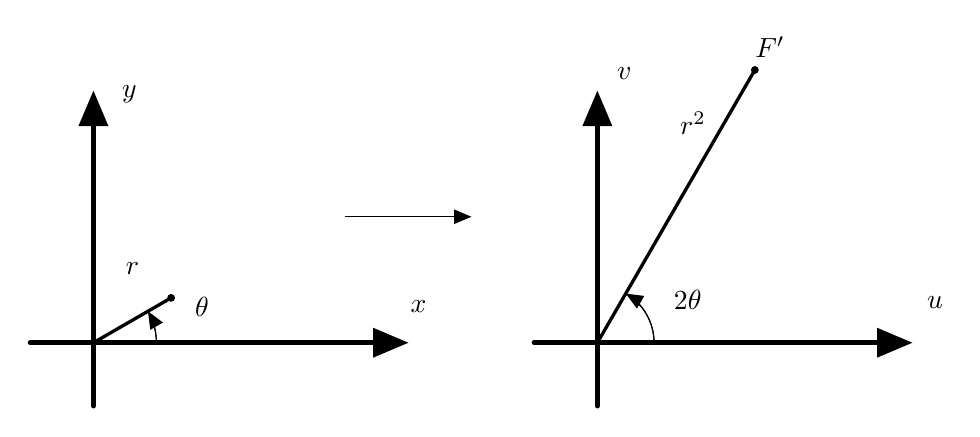
\begin{tikzpicture}[line cap=round,line join=round,>=triangle 45,x=1cm,y=1cm, scale=0.8]
					\draw [shift={(-5,1)},line width=0.4pt] (0,0) -- (0:1) arc (0:30:1) -- cycle;
					\draw [shift={(3,1)},line width=0.4pt] (0,0) -- (0:0.9) arc (0:60:0.9) -- cycle;
					\draw [->,line width=2pt] (-6,1) -- (0,1);
					\draw [->,line width=2pt] (-5,0) -- (-5,5);
					\draw [->,line width=2pt] (2,1) -- (8,1);
					\draw [->,line width=2pt] (3,0) -- (3,5);
					\draw [shift={(-5,1)},->,line width=0.4pt] (0:1) arc (0:30:1);
					\draw [shift={(3,1)},->,line width=0.4pt] (0:0.9) arc (0:60:0.9);
					\draw [->,line width=0.4pt] (-1,3) -- (1,3);
					\draw [line width=1.2pt] (3,1)-- (5.5,5.330127018922193);
					\draw [line width=1.2pt] (-5,1)-- (-3.766891108675446,1.711935750346352);
					\draw (-4.64,2.42) node[anchor=north west] {$r$};
					\draw (4.16,4.82) node[anchor=north west] {$r^2$};
					\draw (-3.54,1.88) node[anchor=north west] {$\theta$};
					\draw (4.06,1.98) node[anchor=north west] {$2\theta$};
					\draw (-0.12,1.82) node[anchor=north west] {$x$};
					\draw (-4.7,5.24) node[anchor=north west] {$y$};
					\draw (8.08,1.88) node[anchor=north west] {$u$};
					\draw (3.16,5.52) node[anchor=north west] {$v$};
					\draw [fill=black] (5.5,5.330127018922193) circle (1.5pt);
					\draw[color=black] (5.74,5.69) node {$F'$};
					\draw [fill=black] (-3.766891108675446,1.711935750346352) circle (1.5pt);
				\end{tikzpicture}
			\end{center}
			
			Note that $f(z) = (re^{i\theta})^2 = r^2e^{i2\theta}$ (angle is doubled)
			\item the strip $1 \leq \Re(z) \leq 2$
			
			With $1 \leq x \leq 2$, the boundaries become: \begin{itemize}
				\item $x = 1 \Rightarrow \begin{dcases}
					u = 1-y^2\\
					v=2y
				\end{dcases} \Rightarrow u = 1 - \big(\dfrac{v}{2}\big)^2$, which is a parabola
				\item $x = 2 \Rightarrow \begin{dcases}
					u = 4-y^2\\
					v=4y
				\end{dcases} \Rightarrow u = 4 - \big(\dfrac{v}{4}\big)^2$, which is a parabola
			\end{itemize}
			\begin{center}
				\definecolor{qqqqff}{rgb}{0,0,1}
				\begin{tikzpicture}[line cap=round,line join=round,>=triangle 45,x=1cm,y=1cm]
					\begin{axis}[
						x=1cm,y=1cm,
						axis lines=middle,
						xmin=-1,
						xmax=4,
						ymin=-1,
						ymax=2,
						xlabel={x} ,
						ylabel={y},
						xtick=\empty,
						ytick=\empty]
					\end{axis}
					\draw[line width=0pt,fill=qqqqff,fill opacity=0.25]
					(2,3)--(2,1)--(3,1)--(3,3);
					\draw[line width=0pt,fill=qqqqff,fill opacity=0.25]
					(2,-1)--(2,1)--(3,1)--(3,-1);
					\draw (3,2) node[anchor=north west] {$x=2$};
					\draw (1,2) node[anchor=north west] {$x=1$};
					\draw [fill=black] (2,1) circle (2pt);
					\draw[color=black] (1.8,0.5) node {1};
					\draw [fill=black] (3,1) circle (2pt);
					\draw[color=black] (3.3,0.5) node {2};
					\draw [fill=black] (2.5,1) circle (2pt);
				\end{tikzpicture}
				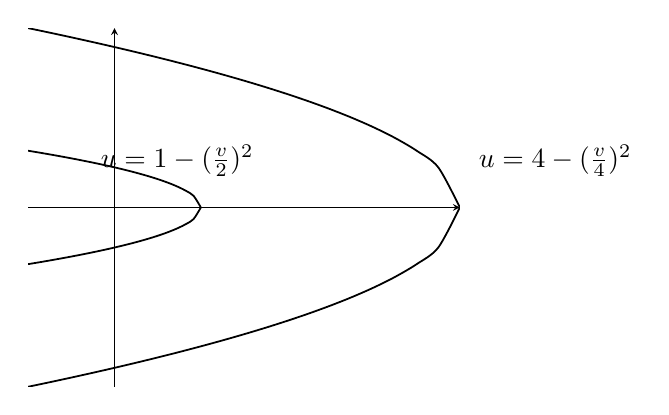
\begin{tikzpicture}[scale=0.8]
					\begin{axis}[
						axis x line=middle,
						axis y line=middle,
						xtick=\empty,
						ytick=\empty
						]
						\addplot[smooth,thick,domain=-1:1]{2*sqrt(1-x)}; 
						\addplot[smooth,thick,domain=-1:1]{-2*sqrt(1-x)};
						\addplot[smooth,thick,domain=-1:5]{4*sqrt(4-x)}; 
						\addplot[smooth,thick,domain=-1:5]{-4*sqrt(4-x)};
					\end{axis}
				\draw (1,4) node[anchor=north west] {$u=1-(\frac{v}{2})^2$};
				\draw (7,4) node[anchor=north west] {$u=4-(\frac{v}{4})^2$};
				\end{tikzpicture}
			\end{center}
		\end{enumerate}
		\item $f(z) = |z|$. This one maps complex plane to non-negative real axis. 
		\begin{center}
			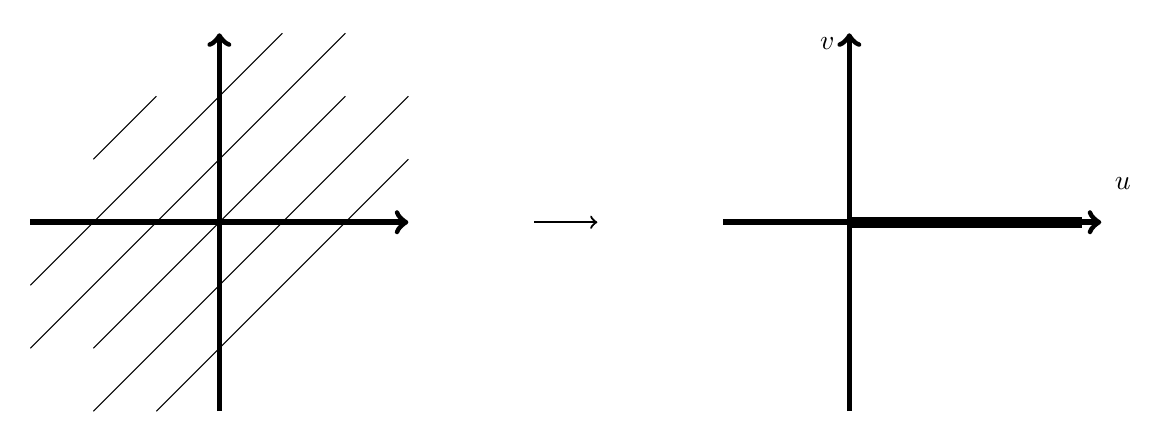
\begin{tikzpicture}[scale=0.8][line cap=round,line join=round,>=triangle 45,x=1cm,y=1cm]
				\draw [->,line width=2pt] (-3,-2) -- (-3,4);
				\draw [->,line width=2pt] (-6,1) -- (0,1);
				\draw [line width=0.4pt] (-4,3)-- (-5,2);
				\draw [line width=0.4pt] (-2,4)-- (-6,0);
				\draw [line width=0.4pt] (-1,4)-- (-6,-1);
				\draw [line width=0.4pt] (0,3)-- (-5,-2);
				\draw [line width=0.4pt] (-4,-2)-- (0,2);
				\draw [->,line width=0.8pt] (2,1) -- (3,1);
				\draw [line width=0.4pt] (-5,-1)-- (-1,3);
				\draw [->,line width=2pt] (5,1) -- (11,1);
				\draw [->,line width=2pt] (7,-2) -- (7,4);
				\draw [line width=4pt] (7,1)-- (10.7,1);
				\draw (11.06,1.86) node[anchor=north west] {$u$};
				\draw (6.38,4.08) node[anchor=north west] {$v$};
			\end{tikzpicture}
		\end{center}
		\item $f(z) = z-z_0 = (x+iy) - (x_0+iy_0) = (x-x_0) + i(y-y_0)$. This is a translation. 
		\item $f(z) = z_0z$, so $$f(z) = r_0e^{i\theta_0}re^{i\theta} = \underbrace{r_0}_{\text{magnification}}re^{i\underbrace{\theta_0}_{\text{rotation}}+\theta} = r_0re^{i\theta_0+\theta}$$
		\item $f(z) = \overline{z} = x-iy \rightarrow \begin{dcases}
			u = x\\
			v = -y
		\end{dcases}$. This is a reflection on $y$-axis. 
		\item Find image of half-plane $\Re(z) \geq 1$ under the map $\omega = f(z) = iz-3i$. 
		
		We can do this step by step. First it's a rotation of $\dfrac{\pi}{2}$ (comes from the first $i$), then its a shift down 3 units. 

		\begin{center}
			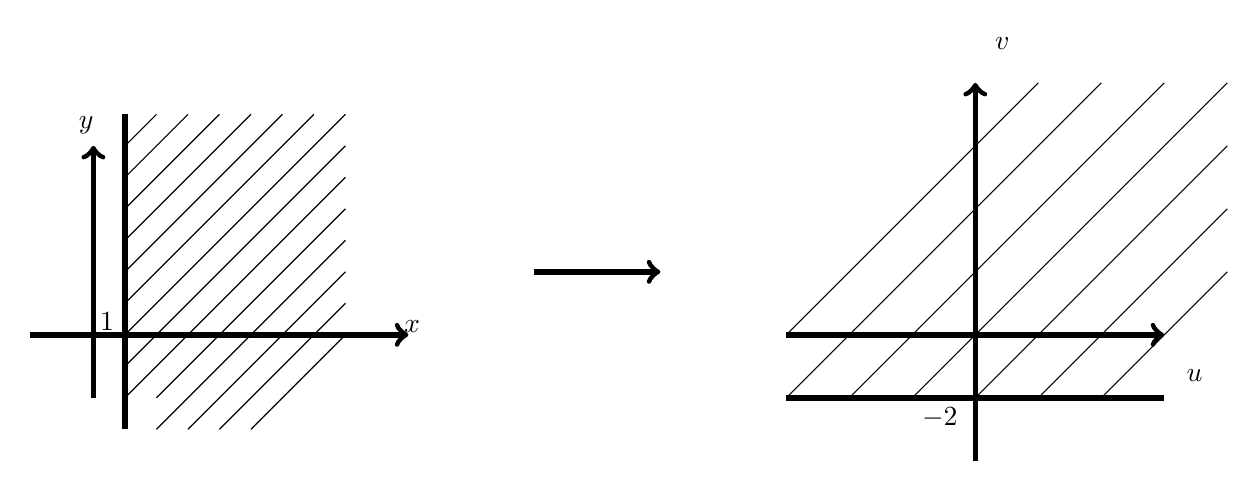
\begin{tikzpicture}[scale=0.4][line cap=round,line join=round,>=triangle 45,x=1cm,y=1cm]
				\draw [line width=2pt] (1,7)-- (1,-2);
				\draw [line width=0.4pt] (1,6)-- (2,7);
				\draw [line width=0.4pt] (1,5)-- (3,7);
				\draw [line width=0.4pt] (1,4)-- (4,7);
				\draw [line width=0.4pt] (1,3)-- (5,7);
				\draw [line width=0.4pt] (1,2)-- (6,7);
				\draw [line width=0.4pt] (1,1)-- (7,7);
				\draw [line width=0.4pt] (1,0)-- (8,7);
				\draw [line width=0.4pt] (1,-1)-- (8,6);
				\draw [line width=0.4pt] (1,-2)-- (8,5);
				\draw [line width=2pt] (1,-2)-- (1,-3);
				\draw [line width=0.4pt] (2,-2)-- (8,4);
				\draw [line width=0.4pt] (2,-3)-- (8,3);
				\draw [line width=0.4pt] (3,-3)-- (8,2);
				\draw [line width=0.4pt] (4,-3)-- (8,1);
				\draw [line width=0.4pt] (5,-3)-- (8,0);
				\draw [->,line width=2pt] (0,-2) -- (0,6);
				\draw [->,line width=2pt] (-2,0) -- (10,0);
				\draw (-0.0975,1) node[anchor=north west] {$1$};
				\draw (-0.7725,7.2375) node[anchor=north west] {$y$};
				\draw (9.555,0.7575) node[anchor=north west] {$x$};
				\draw [->,line width=2pt] (14,2) -- (18,2);
				\draw [->,line width=2pt] (22,0) -- (34,0);
				\draw [line width=2pt] (22,-2)-- (34,-2);
				\draw [->,line width=2pt] (28,-4) -- (28,8);
				\draw [line width=0.4pt] (22,0)-- (30,8);
				\draw [line width=0.4pt] (24,-2)-- (34,8);
				\draw [line width=0.4pt] (26,-2)-- (36,8);
				\draw [line width=0.4pt] (28,-2)-- (36,6);
				\draw [line width=0.4pt] (30,-2)-- (36,4);
				\draw [line width=0.4pt] (32,-2)-- (36,2);
				\draw [line width=0.4pt] (22,-2)-- (32,8);
				\draw (34.395,-0.795) node[anchor=north west] {$u$};
				\draw (28.32,9.735) node[anchor=north west] {$v$};
				\draw (26,-2) node[anchor=north west] {$-2$};
				\begin{scriptsize}
					\draw [fill=black] (28,-2) circle (1.5pt);
				\end{scriptsize}
			\end{tikzpicture}
		\end{center}

		The image is the half-plane $v\geq -2$. 
		\item Inversion mapping. $f(z) = \dfrac{1}{z} = \dfrac{1}{re^{i\theta}} = \dfrac{1}{r}e^{-i\theta}$. So, it's a scaling by $r$, and then reflection through the $x$-axis. 
		
		For this mapping, unit circle maps to the unit circle. Outside points go to inside, and inside points go to outside. 

		\begin{center}
			\definecolor{uuu}{rgb}{0.3,0.3,0.3}
			\begin{tikzpicture}[scale=1.2][line cap=round,line join=round,>=triangle 45,x=1cm,y=1cm]
				\draw [shift={(0,0)},line width=2pt] (0,0) -- (0:0.4193384935264618) arc (0:45:0.4193384935264618) -- cycle;
				\draw [->,line width=1.2pt] (-3,0) -- (3,0);
				\draw [->,line width=1.2pt] (0,-3) -- (0,3);
				\draw [line width=2pt] (0,0) circle (2cm);
				\draw [line width=0.4pt,dash pattern=on 1pt off 1pt] (-2,2)-- (2,-2);
				\draw [line width=0.4pt,dash pattern=on 1pt off 1pt] (-2,-2)-- (2,2);
				\draw [->,line width=1.2pt] (-2,2) -- (-1,-1);
				\draw [->,line width=1.2pt] (1,1) -- (2,-2);
				\draw [->,line width=1.2pt] (1.414213562373095,1.414213562373095) -- (1.414213562373095,-1.414213562373095);
				\begin{scriptsize}
					\draw [fill=uuu] (1.414213562373095,1.414213562373095) circle (1.5pt);
					\draw [fill=uuu] (1.414213562373095,-1.414213562373095) circle (1.5pt);
					\draw [fill=black] (2,-2) circle (1.5pt);
					\draw [fill=black] (1,1) circle (1.5pt);
					\draw [fill=black] (-1,-1) circle (1.5pt);
					\draw [fill=black] (-2,2) circle (1.5pt);
				\end{scriptsize}
			\end{tikzpicture}
		\end{center}

		\item Image of circle $(x-1)^2+y^2 = 1$ under $f(z) = \dfrac{1}{z}$. 
		
		The trick is to use polar fomulas. Recall $x^2+y^2 = r^2, x = r\cos \theta, y = r\sin \theta$. 

		So, $x^2 - 2x + 1 + y^2 = 1$ yields that $r^2 = 2r\cos \theta$. Since $r \neq 0$, we then have $r = 2\cos \theta$. 

		To apply the map, replace $r$ with $\dfrac{1}{r}$, and $\theta$ with $-\theta$: $$\dfrac{1}{r} = 2\cos(-\theta) \Rightarrow r = \dfrac{1}{2\cos \theta}  \Rightarrow r\cos \theta = \dfrac{1}{2}$$
		So $u = \dfrac{1}{2}$ since $\begin{dcases}
			u = r\cos \theta\\
			v = r\sin \theta
		\end{dcases}$ in the uv plane. 

		\begin{center}
			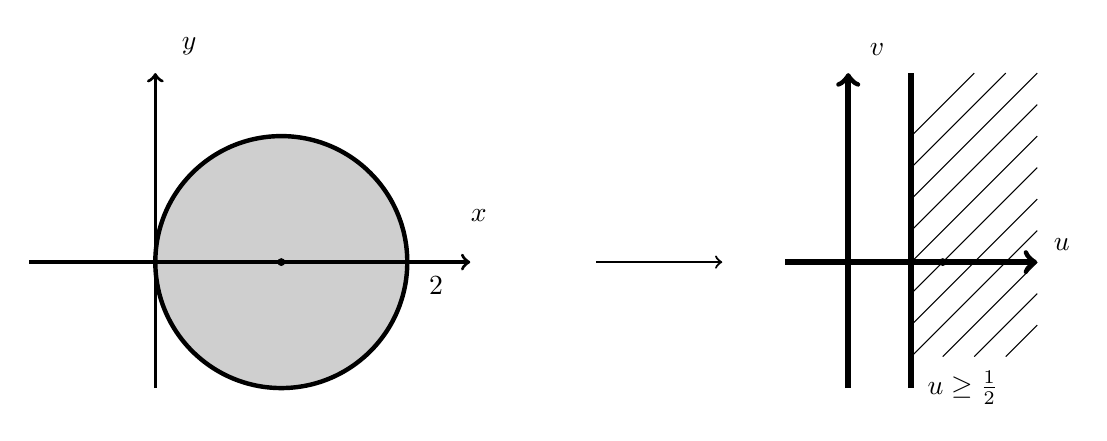
\begin{tikzpicture}[scale=0.8][line cap=round,line join=round,>=triangle 45,x=1cm,y=1cm]
				\draw [line width=1.6pt,fill=black,fill opacity=0.19] (-2,1) circle (2cm);
				\draw [->,line width=1.2pt] (-4,-1) -- (-4,4);
				\draw [->,line width=1.2pt] (-6,1) -- (1,1);
				\draw (0.19197991994709068,0.9164445322718981) node[anchor=north west] {$2$};
				\draw (8.103948156677006,-0.5763796633375331) node[anchor=north west] {$u\ge\frac{1}{2}$};
				\draw [->,line width=0.8pt] (3,1) -- (5,1);
				\draw [->,line width=2pt] (6,1) -- (10,1);
				\draw [->,line width=2pt] (7,-1) -- (7,4);
				\draw [line width=2pt] (8,-1)-- (8,4);
				\draw (-3.7320151085119515,4.712483201107309) node[anchor=north west] {$y$};
				\draw (0.8530877780026902,1.9827475291357777) node[anchor=north west] {$x$};
				\draw (10.108597790781083,1.5349002704529484) node[anchor=north west] {$u$};
				\draw (7.186927579374079,4.627178961358199) node[anchor=north west] {$v$};
				\draw [line width=0.4pt] (8,3)-- (9,4);
				\draw [line width=0.4pt] (8,2)-- (10,4);
				\draw [line width=0.4pt] (8,1)-- (10,3);
				\draw [line width=0.4pt] (8,0)-- (10,2);
				\draw [line width=0.4pt] (8,-0.5)-- (10,1.5);
				\draw [line width=0.4pt] (8.5,-0.5)-- (10,1);
				\draw [line width=0.4pt] (9,-0.5)-- (10,0.5);
				\draw [line width=0.4pt] (9.5,-0.5)-- (10,0);
				\draw [line width=0.4pt] (8,0.5)-- (10,2.5);
				\draw [line width=0.4pt] (8,1.5)-- (10,3.5);
				\draw [line width=0.4pt] (8,2.5)-- (9.5,4);
				\begin{scriptsize}
					\draw [fill=black] (-2,1) circle (1.5pt);
					\draw [fill=black] (8.5,1) circle (1.5pt);
				\end{scriptsize}
			\end{tikzpicture}
		\end{center}

		\item $w = f(z) = \dfrac{z}{z+1}$, find the image of upper-half of unit circle. 
		
		First, $f(z) = \dfrac{z+1-1}{z+1} = 1 - \dfrac{1}{z+1}$. This is a sequence of transformations:$$z \rightarrow \underbrace{z+1}_{\text{shift right}} \rightarrow \underbrace{\dfrac{1}{z+1}}_{\text{invert}} \rightarrow \underbrace{\dfrac{-1}{z+1}}_{\text{reflect and rotate }\pi} \rightarrow \underbrace{1-\dfrac{1}{z+1}}_{\text{shift right}}$$
		\begin{center}
			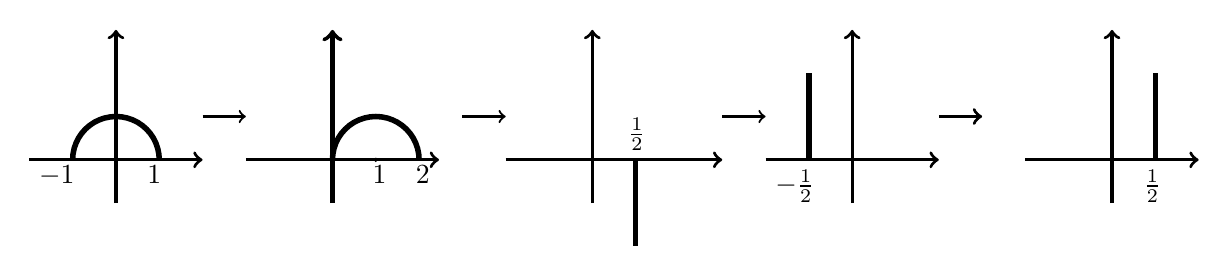
\begin{tikzpicture}[scale=0.55][line cap=round,line join=round,>=triangle 45,x=1cm,y=1cm]
				\draw [->,line width=1.2pt] (-7,0) -- (-3,0);
				\draw [->,line width=1.2pt] (-5,-1) -- (-5,3);
				\draw [->,line width=1.2pt] (-2,0) -- (2.46,0);
				\draw [->,line width=1.6pt] (0,-1) -- (0,3);
				\draw [->,line width=1.2pt] (4,0) -- (9,0);
				\draw [->,line width=1.2pt] (6,-1) -- (6,3);
				\draw [shift={(-5,0)},line width=2pt]  plot[domain=0:3.141592653589793,variable=\t]({1*1*cos(\t r)+0*1*sin(\t r)},{0*1*cos(\t r)+1*1*sin(\t r)});
				\draw [shift={(1,0)},line width=2pt]  plot[domain=0:3.141592653589793,variable=\t]({1*1*cos(\t r)+0*1*sin(\t r)},{0*1*cos(\t r)+1*1*sin(\t r)});
				\draw [->,line width=1.2pt] (10,0) -- (14,0);
				\draw [->,line width=1.2pt] (16,0) -- (20,0);
				\draw [->,line width=1.2pt] (12,-1) -- (12,3);
				\draw [->,line width=1.2pt] (18,-1) -- (18,3);
				\draw [line width=2pt] (7,0)-- (7,-2);
				\draw [line width=2pt] (11,0)-- (11,2);
				\draw [line width=2pt] (19,0)-- (19,2);
				\draw (-7,0.1) node[anchor=north west] {$-1$};
				\draw (-4.5,0.1) node[anchor=north west] {$1$};
				\draw (0.7,0.1) node[anchor=north west] {$1$};
				\draw (1.7,0.1) node[anchor=north west] {$2$};
				\draw (6.6,1.2) node[anchor=north west] {$\frac{1}{2}$};
				\draw (10,0) node[anchor=north west] {$-\frac{1}{2}$};
				\draw (18.5,0) node[anchor=north west] {$\frac{1}{2}$};
				\draw [->,line width=0.8pt] (-3,1) -- (-2,1);
				\draw [->,line width=0.8pt] (3,1) -- (4,1);
				\draw [->,line width=0.8pt] (9,1) -- (10,1);
				\draw [->,line width=1.2pt] (14,1) -- (15,1);
				\begin{scriptsize}
					\draw [fill=black] (1,0) circle (1pt);
				\end{scriptsize}
			\end{tikzpicture}
		\end{center}
	\end{enumerate}
\end{example}
\subsection{Limits and Differentiation}
\begin{definition}
	\underline{\textbf{Limits}}: $$\lim_{z \rightarrow z_0}f(z) = w_0$$ means that for any $\epsilon > 0$, there exists $\delta > 0$ such that $$0 < |z - z_0| < \delta \;\;\; \Rightarrow \;\;\; |f(z)-w_0| < \epsilon$$
\end{definition}
\begin{example}
	Prove that $\lim_{z \rightarrow 1 + i}(2+i)z = 1+3i$.

	\underline{\textbf{Solution}}: We first do some preliminary work: $$|(2+i)z - (1+3i)| = |2+i| \cdot |z-\dfrac{1+3i}{2+i}| = \sqrt{5}\cdot |z - (1+i)|$$
	So, let $\epsilon > 0$, with $|z-z_0| < \dfrac{\epsilon}{\sqrt{5}}(= \delta)$, we have \begin{align*}
		|(2+i)z - (1+3i)| &= \sqrt{5}\cdot|z-(1+i)|\\
		&<\sqrt{5}\cdot\dfrac{\epsilon}{\sqrt{5}}\\
		&=\epsilon
	\end{align*}
	So, $\lim_{z \rightarrow 1 + i}(2+i)z = 1+3i$ \qed
\end{example}
Note that similar definitions apply when dealing with infinity, e.g. $\lim_{z \rightarrow z_0}f(z) = \infty$ means that for any $\epsilon > 0$, there exists $\delta > 0$ such that $0 < |z - z_0| < \delta \;\;\; \Rightarrow \;\;\; |f(z)| > \dfrac{1}{\epsilon}$
\begin{definition}
	\textbf{\underline{Continuity}}: $f$ is \underline{\textbf{continuous}} at $z_0$ means that $$\lim_{z \rightarrow z_0}f(z) = f(z_0)$$
\end{definition}
The usual limit and continuity theorems hold, e.g. $$\lim_{z \rightarrow z_0}f(z)g(z) = \lim_{z \rightarrow z_0}f(z) \cdot \lim_{z \rightarrow z_0}g(z)$$
\begin{theorem}
	Let $f(z) = u + iv, z_0 = x_0 + iy_0, w_0 = u_0 + iv_0$, then $$\lim_{z \rightarrow z_0} f(z) = w_0 \;\;\text{ if and only if }\;\; \begin{dcases}
		\lim_{(x,y) \rightarrow (x_0, y_0)} u(x, y) = u_0\\
		\lim_{(x,y) \rightarrow (x_0, y_0)} v(x, y) = v_0
	\end{dcases}$$
\end{theorem}
\begin{definition}
	\underline{\textbf{Differentiation}}: $$f'(z_0) = \lim_{z \rightarrow z_0} \dfrac{f(z)-f(z_0)}{z - z_0} \bigg(= \lim_{\Delta z \rightarrow 0} \dfrac{f(z_0 + \Delta z) - f(z_0)}{\Delta z}\bigg)$$
	Derivative function is $$f'(z)= \lim_{\Delta z \rightarrow 0} \dfrac{f(z + \Delta z) - f(z)}{\Delta z}$$
\end{definition}
For functions with real analogues (e.g. $f(z) = z^2$ analogous to $f(x) = x^2$), the usual rules (power, quotient, etc.) apply, e.g. $$f(z) = 3z^2+z^4 \;\; \Rightarrow f'(z) = 6z+4z^3$$

What about functions without real analogues? 
\begin{example}
	$f(z) = \overline{z}$. Is it differentiable? 

	\textbf{\underline{Solution}}: 
	\begin{align*}
		f'(z_0) &= \lim_{z \rightarrow z_0}\dfrac{\overline{z} - \overline{z_0}}{z-z_0}\\
		&=\lim_{z \rightarrow z_0} \dfrac{\;\;\;\overline{z-z_0}\;\;\;}{z-z_0}\\
		&=\lim_{z \rightarrow z_0} \dfrac{\;\;\;\overline{re^{i\theta}}\;\;\;}{re^{i\theta}} \;\;\text{ where }\;\; z-z_0 = e^{i\theta}\\
		&=\lim_{z \rightarrow z_0} \dfrac{\;e^{-i\theta}\;}{e^{i\theta}}\\
		&=\lim_{z \rightarrow z_0} e^{-i2\theta}
	\end{align*}
	which depends on $\theta$! No unique value, so limit DNE. So, $f$ is not differentiable anywhere. 
\end{example}
\begin{theorem}
	\underline{\textbf{Cauchy-Riemann Equations}}: If $f(z) = u(x,y) + iv(x,y)$ and $f'(z_0)$ exists, then 
	\begin{tcolorbox}[hbox, before=\par\smallskip\centering]
		$u_x = v_y\;\;$ and $\;\;v_x = -u_y$ $\;\;\;\;\;$ at $(x_0, y_0)$
	\end{tcolorbox}
	Note that for notation, \begin{align*}
		u_x &= \dfrac{\partial u}{\partial x}\\
		u_y &= \dfrac{\partial u}{\partial y}\\
		v_x &= \dfrac{\partial v}{\partial x}\\
		v_y &= \dfrac{\partial v}{\partial y}
	\end{align*}
\end{theorem}
\begin{proof}
	\begin{align*}
		f'(z_0) &= \lim_{\Delta z \rightarrow 0} \dfrac{f(z_0 + \Delta z) - f(z_0)}{\Delta z}\\
		&= \lim_{(\Delta x, \Delta y)  \rightarrow (0, 0)} \bigg( \dfrac{u(x_0 + \Delta x, y_0 + \Delta y) - u(x_0, y_0)}{\Delta x + i \Delta y} + i \dfrac{v(x_0 + \Delta x, y_0 + \Delta y) - v(x_0, y_0)}{\Delta x + i \Delta y} \bigg)
	\end{align*}
	Since the limit exists, it must be independent of path, so \begin{itemize}
		\item Along $\Delta y = 0$: $$f'(z_0) = \lim_{\Delta x \rightarrow 0} \dfrac{u(x_0 + \Delta x, y_0) - u(x_0, y_0)}{\Delta x} + i (\cdots) = \dfrac{\partial u}{\partial x} + i \dfrac{\partial v}{\partial x}$$
		\item Along $\Delta x = 0$: $$f'(z_0) = \lim_{\Delta y \rightarrow 0} \dfrac{u(x_0, y_0+\Delta y) - u(x_0, y_0)}{i\Delta y} + i (\cdots) = -i \dfrac{\partial u}{\partial y} + \dfrac{\partial v}{\partial y}$$
	\end{itemize}
	Equating the real and imaginary part yields the result. 
\end{proof}
\subsection{Differentiability Continued}
\begin{example}
	Is $f(z) = |z|^2$ differentiable? Where? 

	\textbf{\underline{Solution}}: $f(z) = \sqrt{x^2+y^2}^2 = \underbrace{x^2+y^2}_{u} + \underbrace{0}_{v}i$. So, by CRE, we know that $\begin{dcases}
		u_x = v_y & \Rightarrow 2x = 0\\
		v_x = -u_y & \Rightarrow 0 = -2y
	\end{dcases}$

	It's clear that this is satisfied only at $x=y=0$. 

	So, if $(x,y) \neq (0,0)$, i.e. $z \neq 0$, then $f$ is not differentiable. 

	When $z = 0$, $f'(z) = \lim_{\Delta z \rightarrow 0}\dfrac{f(0 + \Delta z) - f(0)}{\Delta z} = \lim_{\Delta z \rightarrow 0} \dfrac{|\Delta z|^2 - 0}{\Delta z} = 0$. This is because $\bigg|\dfrac{|\Delta z|^2}{\Delta z} - 0\bigg| \leq |\Delta z| \rightarrow 0$ as $\Delta z \rightarrow 0$ (by applying the squeeze theorem).  
\end{example}
Hence, CRE are necessary but not sufficient conditions. 
\begin{theorem}
	Let $f$ be defined in some neighborhood of $z_0$. If $u_x, u_y, v_x, v_y$ exist in that neighborhood, satisfying CRE at $z_0$, and are \underline{\textbf{continuous}} at $z_0$, then $f$ is differentiable at $z_0$. 
\end{theorem}
\begin{definition}
	$f(z)$ is \underline{\textbf{analytic at $z_0$}} if $f'(z)$ exists at every point in some neighborhood of $z_0$. 
	
	$f(z)$ is \underline{\textbf{analytic on an open set $S$}} if it is analytic at every point of $S$. 
\end{definition}
\begin{example}
	$f(z) = z^3 = \cdots =\underbrace{(x^3-3xy^2)}_{u(x,y)} + i\underbrace{(3x^2y-y^2)}_{v(x,y)}$.

	We have \begin{align*}
		u_x &= 3x^2-3y^2\\
		u_y &= -6xy\\
		v_x &= 6xy\\
		v_y &= 3x^2-3y^2
	\end{align*}
	So, CRE satisfied everywhere. All partial derivatives are continuous. By theorem, $f$ is differentiable everywhere, so is analytic everywhere. We refer to ``analytic everywhere'' as ``entire''
\end{example}
\begin{example}
	Where is $f(z) = x^2+iy^2$ analytic? 

	We have \begin{align*}
		u_x &= 2x\\
		u_y &= 0\\
		v_x &= 0\\
		v_y &= 2y
	\end{align*}
	We need $x=y$ to satisfy CRE. 
	\begin{itemize}
		\item If $x \neq y$, $f$ is not differentiable, so not analytic. 
		\item If $x = y$, $f$ cannot be analytic because we are not on an open set. 
	\end{itemize}
	So, $f$ is not analytic nowhere. 
\end{example}
\begin{theorem}
	Sums, products, and compositions of analytic functions are also analytic, except when $\div 0$
\end{theorem}
\begin{example}
	$f(z) = \dfrac{z^3+2}{z^2+1}$ is analytic everywhere except at $z = \pm i$.

	$g(z) = f(z^2)$ is analytic everywhere except wherre $z^2 = \pm i$, i.e. except \begin{align*}
		z &= e^{i (\dfrac{n\pi + \pi / 2}{2})}\\
		&= e^{i (n\pi / 2 + \pi / 4)}\\
		&= e^{i (n\pi/4)}, e^{i (n3\pi/4)}, e^{i (n5\pi/4)}, e^{i (n7\pi/4)}\\
		&=\dfrac{1}{\sqrt{2}}+ \dfrac{i}{\sqrt{2}}, -\dfrac{1}{\sqrt{2}}+ \dfrac{i}{\sqrt{2}}, -\dfrac{1}{\sqrt{2}} - \dfrac{i}{\sqrt{2}},\dfrac{1}{\sqrt{2}} - \dfrac{i}{\sqrt{2}},
	\end{align*}
\end{example}
\begin{theorem}
	Suppose $f$ is analytic in a domain $D$. If $f'(z) = 0$ for all $z \in D$, then $f$ is constant in $D$
\end{theorem}
\begin{proof}
	$f'(z) = u_x + iv_x = v_y - iu_y$. So, $f'(z) = 0 \Rightarrow u_x = v_y = 0 = v_y = u_y$. So, $u$ and $v$ are constant, since $D$ is connected. 
\end{proof}
\begin{theorem}
	Suppose $f$ is analytic in a domain $D$. If $|f(z)| = M$ for all $z \in D$, where $M$ is constant, then $f(z)$ is constant in $D$. 
\end{theorem}
\begin{proof}
	$|f(z)|^2 = u^2 + v^2 = M^2$. 

	We differentiate: \begin{itemize}
		\item with respect to $x$: $2uu_x + 2vv_x = 0$ $\;\;$-- (1)
		\item with respect to $y$: $2uu_y + 2vv_y = 0$ $\;\;$-- (2)
	\end{itemize}
	Now $u_x = v_y$, and $v_x = -u_y$, so the (2) gives $-uv_x + vu_x = 0$ $\;\;$-- (3). 

	Multiply (1) by $u_x$. \begin{align*}
		&\;\;\; uu_x^2 + vu_xv_x = 0\\
		& \Rightarrow \; uux^2 + (uv_x)v_x = 0 \;\;\text{ by (3)}\\
		& \Rightarrow \; u(u_x^2+v_x^2) = 0
	\end{align*}
	So, unless $u = 0$ for all $z \in D$, we must have $u_x^2 + v_x^2 = 0$. So, $u_x = v_x = 0$, implying that $u, v$ are constant. Hence, $f$ is constant. 

	What if $u = 0$ for all $z \in D$? Then, $u_x = u_y = 0$, so $v_x = v_y = 0$ by CRE. $f$ is constant as well. 
\end{proof}
\subsection{Harmonic Functions}
Recap: $$f'(z) = u_x + iv_x = \dfrac{u_y+iv_y}{i} = v_y - iu_y$$
$$CRE: \;\;\; u_x = v_y \;\;\;\; v_x = -u_y$$
Also, ``analytic'' means differentiable on a open set. 

Suppose $f(z) = u(x,y) + iv(x,y)$ is analytic in a domain $D$. Then $u$ and $v$ satisfy CRE. 

Also, which will be shown later, $u, v \in C^2$ (continuous under second partial derivatives), and this implies that $u_{xy} = u_{yx}$, and $v_{xy} = v_{yx}$. 

From CRE: $$\underbrace{u_x- v_y}_{\Rightarrow \; u_{xx} = v_{yx}} \;\;\;\; \text{ and } \;\;\;\; \underbrace{v_x = -u_y}_{\Rightarrow \; u_{yy} = -v_{xy}}$$

\begin{definition}
	From the above derivation, we see $$u_{xx}+u_{yy} = v_{yx} - v_{xy} = 0$$ and $$v_{xx} + v_{yy} = 0$$

	We refer to these as \underline{\textbf{``Laplace's equation''}}

	Solution to Laplace's equation are called \underline{\textbf{``harmonic functions''}}
\end{definition}
Notes: \begin{itemize}
	\item We've shown that if $f(z) = u+iv$ is analytic, then $u$ and $v$ must be harmonic
	\item Laplace's equation is very useful! We will see that later. 
	\item $u_{xx} + u_{yy} = 0$ is also denoted as $\Delta^2 u = 0$, and we denote $\Delta$ as ``Laplacian operator''.  
\end{itemize}
\begin{example}
	Suppose $u(x,y) = e^{-2x}\cos 2y + 2y$. Find $v(x,y)$ such that $f(z) = u+iv$ is analytic. 
	
	\underline{\textbf{Solution}}: $u$ and $v$ must satisfy CRE. So, $v_y = u_x = -2e^{-2x}\cos 2y$. Hence, \begin{align*}
		v &= \int -2e^{-2x}\cos 2y dy\\
		&=-e^{2x}\sin 2y +C(x) 
	\end{align*}
	Note that $C(x)$ is a function of all other variables. 
	
	Now we try to make it satisfy other CRE: \begin{align*}
		v_x = -u_y \; &\Rightarrow \; 2e^{-2x}\sin 2y + C'(x) = 2e^{-2x}\sin 2y -2 \\
		&\Rightarrow \; C'(x) = -2\\
		&\Rightarrow \; C(x) = -2x+k
	\end{align*}
	Therefore, $v(x,y) = -e^{-2x}\sin 2y -2x + k$
\end{example}

Note that $v(x,y)$ is called the ``harmonic conjugate'' of $u$. 

Exercise: show that if $v$ is the harmonic conjugate of $u$, then $-u$ is the harmonic conjugate of $v$. 

\begin{example}
	Solve Laplace's equation $\Phi_{xx} + \Phi_{yy} = 0$ on region between hyperbolas $x^2 - y^2 = 1$ and $x^2 - y^2 = 4$, $x > 0$, with ``boundary conditions'' $$\begin{dcases}
		\Phi = 0 & \text{on }x^2-y^2 = 1\\
		\Phi = 10 & \text{on }x^2-y^2 = 4
	\end{dcases}$$
	i.e. Find $\Phi(x, y)$

	\begin{center}
		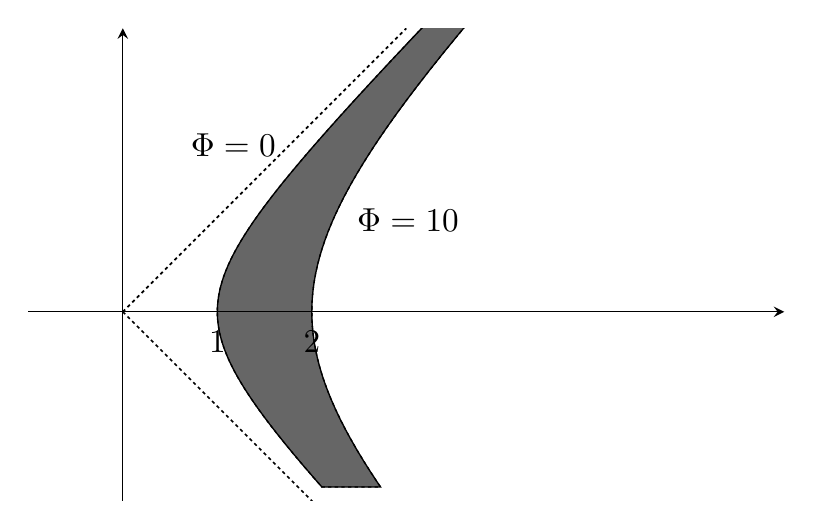
\begin{tikzpicture}[scale=1.2]
			\begin{axis}[
				x=1cm,y=1cm,
				axis lines=middle,
				xmin=-1,
				xmax=7,
				ymin=-2,
				ymax=3,
				xtick={0,1,2},
				ytick=\empty,]
				\draw[line width=0.4pt,dash pattern=on 1pt off 1pt,fill=black,fill opacity=0.37](3.274662080624353,3.11793063089423)--(3.078142092260624,2.9111782391579215)--(2.8331024958925553,2.65074890403309)--(2.62235876612791,2.424204095840096)--(2.439457643220119,2.2250738399129717)--(2.2794823017751518,2.04842367788164)--(2.1386215920525538,1.8904238450658102)--(2.013876570275504,1.7480557314641392)--(1.902855849728697,1.6189071575747387)--(1.8036299216591194,1.5010266134562968)--(1.7146255358809155,1.3928175502537714)--(1.6345478583034294,1.2929604406494146)--(1.5623222466932392,1.2003544486994708)--(1.4970501151013949,1.1140731785323166)--(1.4379750703709617,1.0333306842479673)--(1.3844566424842901,0.9574550615662721)--(1.3359497007199626,0.8858677118248286)--(1.2919881773739395,0.818066898532164)--(1.2521720907696334,0.7536145864448188)--(1.2161571212858309,0.692125814902348)--(1.1836461820996187,0.6332600448465099)--(1.154382562835803,0.5767140551255507)--(1.1281443245617162,0.5222160635606788)--(1.1047396989865015,0.4695208222398513)--(1.0840033005398864,0.41840549181549586)--(1.0657930022854967,0.36866614127247027)--(1.0499873589659243,0.3201147512818441)--(1.0364834854637945,0.27257662342757116)--(1.025195318469489,0.22588811613663334)--(1.0160522045474452,0.1798946424041676)--(1.0089977701103137,0.1344488753675005)--(1.0039890388117536,0.08940911616915155)--(1.0009957701407863,0.044637784888429025)--(1,0)--(1.0009957701407863,-0.044637784888429025)--(1.0039890388117536,-0.08940911616915155)--(1.0089977701103137,-0.1344488753675005)--(1.0160522045474452,-0.1798946424041676)--(1.025195318469489,-0.22588811613663334)--(1.0364834854637945,-0.27257662342757116)--(1.0499873589659243,-0.3201147512818441)--(1.0657930022854967,-0.36866614127247027)--(1.0840033005398864,-0.41840549181549586)--(1.1047396989865015,-0.4695208222398513)--(1.1281443245617162,-0.5222160635606788)--(1.154382562835803,-0.5767140551255507)--(1.1836461820996187,-0.6332600448465099)--(1.2161571212858309,-0.6921258149023477)--(1.2521720907696334,-0.7536145864448188)--(1.2919881773739395,-0.8180668985321636)--(1.3359497007199626,-0.8858677118248286)--(1.3844566424842901,-0.9574550615662718)--(1.4379750703709617,-1.0333306842479673)--(1.4970501151013949,-1.1140731785323166)--(1.5623222466932392,-1.2003544486994708)--(1.6345478583034294,-1.2929604406494148)--(1.7146255358809155,-1.392817550253771)--(1.8036299216591194,-1.501026613456297)--(1.902855849728697,-1.6189071575747385)--(2.013876570275504,-1.7480557314641394)--(2.106493985617573,-1.853757478283976)--(2.7272960359541996,-1.853757478283976)--(2.705031186697621,-1.8213164801886406)--(2.6215420882179234,-1.6948400869397646)--(2.545247951175891,-1.5742576450394234)--(2.475585301839686,-1.4589457106707866)--(2.4120621868658976,-1.3483486171270012)--(2.354248395352079,-1.241968400168796)--(2.3017673458053984,-1.1393563596241645)--(2.2542893280972573,-1.040105944013966)--(2.2115258561439055,-0.943846710219957)--(2.1732249376845645,-0.8502391603390652)--(2.1391671068871294,-0.7589702966439806)--(2.1091620963576054,-0.6697497657421086)--(2.0830460495047594,-0.5823064866179866)--(2.0606791936405027,-0.4963856757631847)--(2.0419439098274945,-0.41174619716713284)--(2.0267431481919322,-0.3281581764072716)--(2.0149991478729583,-0.24540082707429625)--(2.0066524295027275,-0.16326044477827598)--(2.0016610355153692,-0.08152852936525122)--(2,0)--(2.0016610355153692,0.08152852936525122)--(2.0066524295027275,0.16326044477827598)--(2.0149991478729583,0.24540082707429625)--(2.0267431481919322,0.3281581764072716)--(2.0419439098274945,0.41174619716713284)--(2.0606791936405027,0.4963856757631847)--(2.0830460495047594,0.5823064866179866)--(2.1091620963576054,0.6697497657421086)--(2.1391671068871294,0.7589702966439806)--(2.1732249376845645,0.8502391603390652)--(2.2115258561439055,0.943846710219957)--(2.2542893280972573,1.040105944013966)--(2.3017673458053984,1.1393563596241647)--(2.354248395352079,1.241968400168796)--(2.4120621868658976,1.3483486171270014)--(2.475585301839686,1.4589457106707866)--(2.545247951175891,1.5742576450394234)--(2.6215420882179234,1.6948400869397648)--(2.705031186697621,1.8213164801886406)--(2.796362079425364,1.9543901553293148)--(2.8962793668882174,2.094858985961207)--(3.005643055848226,2.2436332541591244)--(3.1254502909692925,2.4017575900411)--(3.2568623181918555,2.570438126012377)--(3.401238197238152,2.751076384681428)--(3.560177306884961,2.945311945526085)--(3.704513524284938,3.11793063089423);
				\draw[line width=0.4pt,fill=black,fill opacity=0.37](3.274662080624353,3.11793063089423)--(3.078142092260624,2.9111782391579215)--(2.8331024958925553,2.65074890403309)--(2.62235876612791,2.424204095840096)--(2.439457643220119,2.2250738399129717)--(2.2794823017751518,2.04842367788164)--(2.1386215920525538,1.8904238450658102)--(2.013876570275504,1.7480557314641392)--(1.902855849728697,1.6189071575747387)--(1.8036299216591194,1.5010266134562968)--(1.7146255358809155,1.3928175502537714)--(1.6345478583034294,1.2929604406494146)--(1.5623222466932392,1.2003544486994708)--(1.4970501151013949,1.1140731785323166)--(1.4379750703709617,1.0333306842479673)--(1.3844566424842901,0.9574550615662721)--(1.3359497007199626,0.8858677118248286)--(1.2919881773739395,0.818066898532164)--(1.2521720907696334,0.7536145864448188)--(1.2161571212858309,0.692125814902348)--(1.1836461820996187,0.6332600448465099)--(1.154382562835803,0.5767140551255507)--(1.1281443245617162,0.5222160635606788)--(1.1047396989865015,0.4695208222398513)--(1.0840033005398864,0.41840549181549586)--(1.0657930022854967,0.36866614127247027)--(1.0499873589659243,0.3201147512818441)--(1.0364834854637945,0.27257662342757116)--(1.025195318469489,0.22588811613663334)--(1.0160522045474452,0.1798946424041676)--(1.0089977701103137,0.1344488753675005)--(1.0039890388117536,0.08940911616915155)--(1.0009957701407863,0.044637784888429025)--(1,0)--(1.0009957701407863,-0.044637784888429025)--(1.0039890388117536,-0.08940911616915155)--(1.0089977701103137,-0.1344488753675005)--(1.0160522045474452,-0.1798946424041676)--(1.025195318469489,-0.22588811613663334)--(1.0364834854637945,-0.27257662342757116)--(1.0499873589659243,-0.3201147512818441)--(1.0657930022854967,-0.36866614127247027)--(1.0840033005398864,-0.41840549181549586)--(1.1047396989865015,-0.4695208222398513)--(1.1281443245617162,-0.5222160635606788)--(1.154382562835803,-0.5767140551255507)--(1.1836461820996187,-0.6332600448465099)--(1.2161571212858309,-0.6921258149023477)--(1.2521720907696334,-0.7536145864448188)--(1.2919881773739395,-0.8180668985321636)--(1.3359497007199626,-0.8858677118248286)--(1.3844566424842901,-0.9574550615662718)--(1.4379750703709617,-1.0333306842479673)--(1.4970501151013949,-1.1140731785323166)--(1.5623222466932392,-1.2003544486994708)--(1.6345478583034294,-1.2929604406494148)--(1.7146255358809155,-1.392817550253771)--(1.8036299216591194,-1.501026613456297)--(1.902855849728697,-1.6189071575747385)--(2.013876570275504,-1.7480557314641394)--(2.106493985617573,-1.853757478283976)--(2.7272960359541996,-1.853757478283976)--(2.705031186697621,-1.8213164801886406)--(2.6215420882179234,-1.6948400869397646)--(2.545247951175891,-1.5742576450394234)--(2.475585301839686,-1.4589457106707866)--(2.4120621868658976,-1.3483486171270012)--(2.354248395352079,-1.241968400168796)--(2.3017673458053984,-1.1393563596241645)--(2.2542893280972573,-1.040105944013966)--(2.2115258561439055,-0.943846710219957)--(2.1732249376845645,-0.8502391603390652)--(2.1391671068871294,-0.7589702966439806)--(2.1091620963576054,-0.6697497657421086)--(2.0830460495047594,-0.5823064866179866)--(2.0606791936405027,-0.4963856757631847)--(2.0419439098274945,-0.41174619716713284)--(2.0267431481919322,-0.3281581764072716)--(2.0149991478729583,-0.24540082707429625)--(2.0066524295027275,-0.16326044477827598)--(2.0016610355153692,-0.08152852936525122)--(2,0)--(2.0016610355153692,0.08152852936525122)--(2.0066524295027275,0.16326044477827598)--(2.0149991478729583,0.24540082707429625)--(2.0267431481919322,0.3281581764072716)--(2.0419439098274945,0.41174619716713284)--(2.0606791936405027,0.4963856757631847)--(2.0830460495047594,0.5823064866179866)--(2.1091620963576054,0.6697497657421086)--(2.1391671068871294,0.7589702966439806)--(2.1732249376845645,0.8502391603390652)--(2.2115258561439055,0.943846710219957)--(2.2542893280972573,1.040105944013966)--(2.3017673458053984,1.1393563596241647)--(2.354248395352079,1.241968400168796)--(2.4120621868658976,1.3483486171270014)--(2.475585301839686,1.4589457106707866)--(2.545247951175891,1.5742576450394234)--(2.6215420882179234,1.6948400869397648)--(2.705031186697621,1.8213164801886406)--(2.796362079425364,1.9543901553293148)--(2.8962793668882174,2.094858985961207)--(3.005643055848226,2.2436332541591244)--(3.1254502909692925,2.4017575900411)--(3.2568623181918555,2.570438126012377)--(3.401238197238152,2.751076384681428)--(3.560177306884961,2.945311945526085)--(3.704513524284938,3.11793063089423);
				\draw [line width=0.5pt,dash pattern=on 1pt off 1pt] (0,0)-- (3,3);
				\draw [line width=0.5pt,dash pattern=on 1pt off 1pt] (0,0)-- (3,-3);
				\draw (0.5948081886474288,2.0078399652952794) node[anchor=north west] {$\Phi=0$};
				\draw (2.3567061247556373,1.210851795121674) node[anchor=north west] {$\Phi=10$};
			\end{axis}
		\end{tikzpicture}
	\end{center}

	\underline{\textbf{Solution}}: Consider $f(z) = z^2 = (x+yi)^2 = \underbrace{x^2-y^2}_{u(x,y)} + i\underbrace{2xy}_{v(x,y)}$

	Since $f(z)$ is already analytic, we have that $u(x,y) = x^2-y^2$ is harmonic. Boundary curves of region are level curves of a harmonic function. 

	Is the solution $\Phi(x,y) = x^2-y^2$? No. 

	Try $\Phi(x, y) = A\cdot (x^2-y^2)+B$ (also harmonic by linearity). 

	Applying the Boundary Conditions: \begin{align*}
		0 = A \cdot 1 + B & \Rightarrow \; B = -A\\
		10 = A \cdot 4 + B & \Rightarrow \; A = \dfrac{10}{3}, B = -\dfrac{10}{3}
	\end{align*}
	So the solution is $\Phi(x,y) = \dfrac{10}{3}(x^2-y^2)-\dfrac{10}{3}$
\end{example}
Notes: \begin{itemize}
	\item It can be used in temperature distribution
	\item What about more complicated regions? 
	\item Orthogonal trajectories
	\begin{center}
		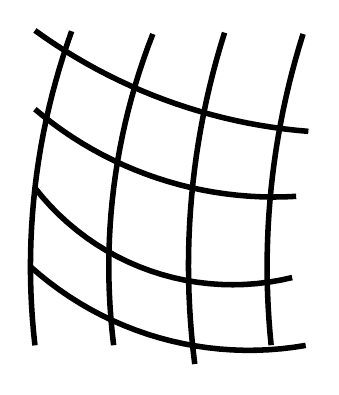
\begin{tikzpicture}
			\draw [shift={(2.7532914746964243,1)},line width=2pt]  plot[domain=2.7953545897816907:3.2553422400667853,variable=\t]({1*8.810227672483448*cos(\t r)+0*8.810227672483448*sin(\t r)},{0*8.810227672483448*cos(\t r)+1*8.810227672483448*sin(\t r)});
			\draw [shift={(3.0271301929022627,1)},line width=2pt]  plot[domain=2.76757136404437:3.2655316496383815,variable=\t]({1*8.08917913844187*cos(\t r)+0*8.08917913844187*sin(\t r)},{0*8.08917913844187*cos(\t r)+1*8.08917913844187*sin(\t r)});
			\draw [shift={(5.74915387214404,1.0113464410519617)},line width=2pt]  plot[domain=2.834591536362894:3.269482313515557,variable=\t]({1*9.799154916744698*cos(\t r)+0*9.799154916744698*sin(\t r)},{0*9.799154916744698*cos(\t r)+1*9.799154916744698*sin(\t r)});
			\draw [shift={(6.749743314584557,1)},line width=2pt]  plot[domain=2.835272950547197:3.2438020438334467,variable=\t]({1*9.800892546104476*cos(\t r)+0*9.800892546104476*sin(\t r)},{0*9.800892546104476*cos(\t r)+1*9.800892546104476*sin(\t r)});
			\draw [shift={(-1.987135331002164,9.525729337995672)},line width=2pt]  plot[domain=4.084285192044407:4.633375921958299,variable=\t]({1*6.829111770096987*cos(\t r)+0*6.829111770096987*sin(\t r)},{0*6.829111770096987*cos(\t r)+1*6.829111770096987*sin(\t r)});
			\draw [shift={(-2.965009369560112,6.569981260879775)},line width=2pt]  plot[domain=4.007812545169585:4.773068445264867,variable=\t]({1*4.68571598903419*cos(\t r)+0*4.68571598903419*sin(\t r)},{0*4.68571598903419*cos(\t r)+1*4.68571598903419*sin(\t r)});
			\draw [shift={(-3.4892419868854327,3.9479739763179724)},line width=2pt]  plot[domain=3.801434135672984:4.952857222143927,variable=\t]({1*3.1778150375424716*cos(\t r)+0*3.1778150375424716*sin(\t r)},{0*3.1778150375424716*cos(\t r)+1*3.1778150375424716*sin(\t r)});
			\draw [shift={(-3.280269756608991,4.0959324511562984)},line width=2pt]  plot[domain=3.9813027208426544:4.88633150707663,variable=\t]({1*4.158686603687145*cos(\t r)+0*4.158686603687145*sin(\t r)},{0*4.158686603687145*cos(\t r)+1*4.158686603687145*sin(\t r)});
		\end{tikzpicture}
	\end{center}
	\item list of harmonic functions
\end{itemize}

\section{Elementary Functions}
\subsection{Elementary Functions}
\begin{definition}
	\underline{\textbf{Polynomials}}: 
	$$p(z) = a_0 + a_1z + a_2z^2 + \cdots + a_nz^n \;,\;\;\; a_i\in \mathbb{C}$$
	They are obviously \underline{\textbf{entire}}. 

	The fundamental theorem of algebra guarantees that we can factor this as $$p(z) = a_n(z-z_1)(z-z_2) \cdots (z-z_n)$$
	Note that $z_i$ are not necessarily distinct. 

	$z_0$ is a ``zero of multiplicity'' $k$ if and only if $$p(z) = (z - z_0)^kq(z)$$ where $q(z)$ is a polynomial such that $q(z_0) \neq 0$
\end{definition}
\begin{definition}
	\underline{\textbf{Rational Functions}}: 
	$$R(z) = \dfrac{p(z)}{q(z)} = \dfrac{a_n(z-z_1)(z-z_2)\cdots(z-z_n)}{b_m(z-w_1)(z-w_2)\cdots (z-w_n)}$$
	Suppose all common factors have been cancelled, then \begin{itemize}
		\item the roots (or zeroes) of $p(z)$ are called the \underline{\textbf{roots/zeroes}} of $R(z)$
		\item the roots (or zeroes) of $q(z)$ are called the \underline{\textbf{poles}} of $R(z)$
	\end{itemize}
\end{definition}
\begin{example}
	$$R(z) = \dfrac{3i(z-1)(z-\frac{1}{3}i)^2(z+i)}{(z-i)^3(z-2-i)}$$
	Zeroes at 1 and $-i$ (order 1 would be a ``simple zero''), and $\dfrac{1}{3}i$ (order 2). 

	Poles at $i$ (order 3) and $2+i$ (order 1 would be a ``simple pole'')
\end{example}
Partial Fractions has simpler rules: 
\begin{example}
	Decompose $R(z) = \dfrac{1}{(z+4)^2(z^2+1)}$

	\underline{\textbf{Solution}}: Factor and expand $$\dfrac{1}{(z+4)^2(z^2+1)} = \dfrac{A}{z+4} + \dfrac{B}{(z+4)^2} + \dfrac{C}{z+i}+\dfrac{D}{z-i}$$
	This gives us $$1 = A\cdot (z+4)(z+i)(z-i) + B(z+i)(z-i) + C(z+4)^2(z-i) + D(z+4)^2(z+i)$$
	We can solve this by: \begin{itemize}
		\item set $z = -4$, this gives us $1 = 0 + (-4+i)(-4-i)B +0+0$, so $B = \dfrac{1}{17}$
		\item set $z = -i$, this gives us $1 = 0 + 0 + (-i+4)^2(-2i)C +0$. Then we compute $(-2i)(15-8i) = 16-30i$, also $(-16-30i) = \dfrac{(-16-30i)(-16+30i)}{(-16+30i)} = \dfrac{1156}{(-16+30i)} = \dfrac{578}{-8+15i}$. 
		
		Hence, $C = \dfrac{-8+15i}{578}$. 
		\item set $z = -4$, this gives us $1 = 0 + 0+0+ (i+4)^2(2i)D$, so $D = \dfrac{-8-15i}{578}$. The trick to compute things here is that, we can replace $i$ with $-i$ from $C$ since the expression is similar to $C$. 
	\end{itemize}
	Now what about $A$? We can try another $z$, or just compare the coefficients of $z^3$. By comparing the coefficients of $z^3$, we get that $$0 + A + C + D = A + \dfrac{-8+15i}{578} + \dfrac{-8-15i}{578}$$ So $A = \dfrac{16}{578} = \dfrac{8}{289}$

	Hence, $$\dfrac{1}{(z+4)^2(z^2+1)} = \dfrac{8/289}{z+4} +\dfrac{1/17}{(z+4)^2} + \dfrac{\frac{-8+15i}{578}}{z+i}+\dfrac{\frac{-8-15i}{578}}{z-i}$$
\end{example}
Actually, often we will only need one of the coefficients, and there's a quick way which will be covered later in the course. 
\begin{definition}
	\underline{\textbf{Exponential Function}}: We already defined that $e^z = e^{x+iy} = e^x(\cos y + i\sin y)$. 

	Note that $e^{z_1+z_2} = e^{z_1}e^{z_2}$, $\dfrac{d}{dz} e^z= e^z$. Also, $e^z$ is \underline{\textbf{periodic}} with period $2\pi i$
\end{definition}
\begin{definition}
	\underline{\textbf{Hyperbolic Functions}}: From real calculus, we seen that \begin{align*}
		\cosh x &= \dfrac{1}{2}(e^x+e^{-x}) \;\;\;\text{ this is the even component of }e^x\\
		\sinh x &= \dfrac{1}{2}(e^x-e^{-x}) \;\;\;\text{ this is the odd component of }e^x
	\end{align*}
	It can be shown that \begin{align*}
		&\cosh x + \sinh x = e^x\\
		&\cosh^2 x - \sinh^2 x = 1\\
		&\dfrac{d}{dx} \sinh x = \cosh x\\
		&\dfrac{d}{dx} \cosh x = \sinh x
	\end{align*}
	\begin{center}
		\begin{tikzpicture}
			\begin{axis}[
				axis lines = middle,
				xlabel = $x$,
				ylabel = {$y$},
				xtick=\empty,
				ytick=\empty,
				legend style={at={(1.5,0.5)},anchor=south east}
				]
				\addplot [
				domain=-1:1, 
				samples y = 0,
				color=blue,
				]
				{cosh(x)};
				\addlegendentry{$\cosh(x)$}
				\addplot [
				domain=-1:1, 
				samples y = 0, 
				color=red
				]
				{0.5*e^x};
				\addlegendentry{$\frac{e^x}{2}$}
				\addplot [
				domain=-1:1, 
				samples y = 0, 
				color = brown
				]
				{0.5*e^(-x)};	
				\addlegendentry{$-\frac{e^x}{2}$}
			\end{axis}
		\end{tikzpicture}
		
		\begin{tikzpicture}
			\begin{axis}[
				axis lines = middle,
				xlabel = $x$,
				ylabel = {$y$},
				xtick=\empty,
				ytick=\empty,
				legend style={at={(1.5,0.5)},anchor=south east}
				]
				\addplot [
				domain=-2:2, 
				samples y = 0,
				color=blue,
				]
				{sinh(x)};
				\addlegendentry{$\sinh(x)$}
				\addplot [
				domain=-2:2, 
				samples y = 0, 
				color=red,
				]
				{0.5*e^x};
				\addlegendentry{$\frac{e^{x}}{2}$}
				\addplot [
				domain=-2:2, 
				samples y = 0, 
				color=brown,
				]
				{-0.5*e^(-x)};
				\addlegendentry{$-\frac{e^{-x}}{2}$}	
			\end{axis}
		\end{tikzpicture}
	\end{center}
	To extend these to $\mathbb{C}$, we define 
	\begin{tcolorbox}[hbox, before=\par\smallskip\centering]
		$\cosh z = \dfrac{1}{2}(e^z+e^{-z}) \;\;\; \sinh z = \dfrac{1}{2}(e^z-e^{-z})$
	\end{tcolorbox}
\end{definition}
\subsection{Trigonometric and Logarithmic Function}
\begin{definition}
	\underline{\textbf{Trigonometric Functions}}: Recall \begin{align*}
		e^{i\theta} &= \cos \theta + i\sin \theta\\
		e^{-i\theta} &= \cos \theta - i\sin \theta
	\end{align*}
	Sum to get $\cos \theta = \dfrac{e^{i\theta} + e^{-i\theta}}{2}$, and $\sin \theta = \dfrac{e^{i\theta} - e^{-i\theta}}{2i}$

	We define \begin{tcolorbox}[hbox, before=\par\smallskip\centering]
		$\cos z = \dfrac{1}{2}(e^{iz}+e^{-iz})= \cosh (iz) \;\;\; \sin z = \dfrac{1}{2i}(e^{iz}-e^{-iz}) = \dfrac{1}{i}\sinh (iz)$
	\end{tcolorbox}
\end{definition}
Furthermore: \begin{align*}
	\cos(iz) &= \dfrac{e^{-z}+e^z}{2} = \cosh z\\
	\sin(iz) &= \dfrac{e^{-z}-e^z}{2i} = i\sinh z
\end{align*}
\begin{align*}
	\text{ For real }z,\;\;\; e^z &= e^x = \cosh x + \sinh x\\
	\text{ For imaginary }z,\;\;\; e^z &= e^{iy} = \cos y + i\sin y
\end{align*}
The $\cosh x$ and $\cos y$ are the even parts, and $\sinh x$ and $i\sin y$ are the odd parts
\begin{center}
	\begin{tabular}{c|c|c}
		Functions & Along Real Axis & Along Imaginary Axis\\
		\hline
		$e^{iz}, \cos z, \sin z$ & periodic & grow exponentially\\
		$e^{z}, \cosh z, \sinh z$ & grow exponentially & periodic
	\end{tabular}
\end{center}
Familiar identities hold true. 
\begin{example}
	\begin{align*}
		\cos^4 \theta &= \left(\dfrac{e^{i\theta} + e^{-i\theta}}{2}\right)^4\\
		&=\dfrac{1}{16}(e^{i4\theta} + 4e^{2\theta} + 6 + 4e^{-i2\theta} + e^{-i4\theta})\\
		&=\dfrac{1}{8} \cos 4 \theta + \dfrac{1}{2}\cos 2\theta + \dfrac{3}{8}
	\end{align*}
\end{example}
\begin{example}
	\begin{align*}
		&\cos^2 \theta + \sin^2 \theta = 1\\
		\Rightarrow\; &\cos^2(iy) + \sin^2 (iy) = 1\\
		\Rightarrow\; &\cosh^2 y + i^2\sinh^2 y = 1\\
		\Rightarrow\; &\cosh^2 y - \sinh^2 y = 1
	\end{align*}
	By using the rules $\begin{dcases}
		\cos(iz) = \cosh z\\
		\sin(iz) = i \sinh z 
	\end{dcases}$.

	Notice the ``Obsborne's rule'' here: Hyperbolic function satisfy the same identities as trigonometric functions except that \underline{we must change the sign of every product of two sines}. 
\end{example}
Derivatives: $e^z$ is entire, and so is $\cos z, \sin z, \cosh z, \sinh z$. Also, $$\dfrac{d}{dz}(\cos z) = \dfrac{d}{dz}(\dfrac{e^{iz}+e^{-iz}}{2}) = \dfrac{ie^{iz}-ie^{-iz}}{2} = \dfrac{e^{iz}-e^{-iz}}{-2i} = -\sin z$$
Other as expected as well

Note: we can also define $\tan z$, $\sec z$ etc. in the usual ways, and derivatives of them are as expected. 
\begin{example}
	What is the value of $\sin(\pi + i)$? 

	\underline{\textbf{Solution}}: \begin{align*}
		\sin(\pi + i) &= \sin \pi \cos (i \cdot 1) + \cos \pi \sin (i \cdot 1)\\
		&= \sin \pi \cosh 1 + \cos \pi i\sinh (1)\\
		&= 0 + (-1) \cdot i \cdot \sinh (1)\\
		&= -\sin i
	\end{align*} 
\end{example}
\begin{example}
	Find all solutions of $\sin z = 1000$

	\textbf{\underline{Solution}}: We write $\sin (x + yi) = 1000$, and get that $$\sin x \cosh y + i \cos x \sinh y = 1000$$
	So $$\begin{dcases}
		\sin x \cosh y = 1000 & \cdots \cdots(1)\\
		\cos x \sinh y = 0 & \cdots \cdots(2)
	\end{dcases}$$
	Equation 2 gives that $\cos x = 0$ or $\sinh y = 0$, which yields that $x = (2n+1)\dfrac{\pi}{2}$ or $y = 0$. 

	The following figure shows that the only $x$ that $\sinh(x) = 0$ is at $x=0$. 
	\begin{center}
		\begin{tikzpicture}
			\begin{axis}[
				axis lines = middle,
				xlabel = $y$,
				ylabel = {$\frac{e^y-e^{-y}}{2}$},
				xtick=\empty,
				ytick=\empty,
				]
				\addplot [
				domain=-2:2, 
				samples y = 0,
				color=blue,
				]
				{sinh(x)};
				\addplot [
				domain=-2:2, 
				samples y = 0, 
				dash pattern=on 1pt off 1pt
				]
				{0.5*e^x};
				\addplot [
				domain=-2:2, 
				samples y = 0, 
				dash pattern=on 1pt off 1pt
				]
				{-0.5*e^(-x)};
				\draw [fill=black] (0,0) circle (2pt);
			\end{axis}
		\end{tikzpicture}
	\end{center}

	\begin{itemize}
		\item If $y = 0$, equation 1 gives that $\sin x \cosh (0) = \sin x = 1000$. This is impossible
		\item If $x = (2n+1)\dfrac{\pi}{2}$, then equation 1 gives $\sin\bigg((2n+1)\dfrac{\pi}{2}\bigg) \cosh y = 1000$, so $\cosh y = 1000 \cdot (-1)^n$
		
		\begin{center}
			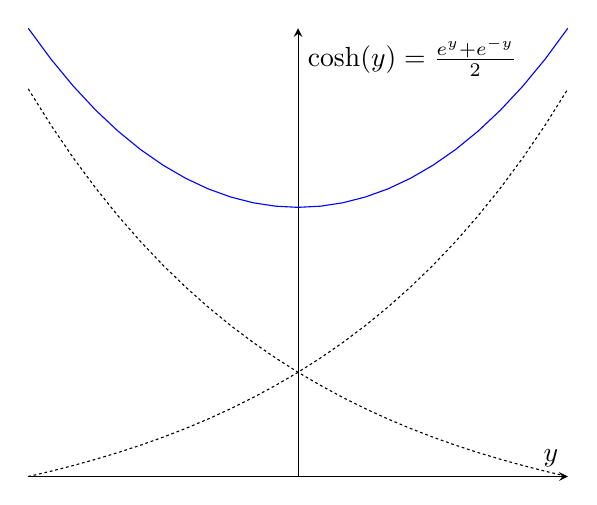
\begin{tikzpicture}
				\begin{axis}[
					axis lines = middle,
					xlabel = $y$,
					ylabel = {$\cosh(y)=\frac{e^y+e^{-y}}{2}$},
					xtick=\empty,
					ytick=\empty,
					legend style={at={(1.5,0.5)},anchor=south east}
					]
					\addplot [
					domain=-1:1, 
					samples y = 0,
					color=blue,
					]
					{cosh(x)};
					\addplot [
					domain=-1:1, 
					samples y = 0, 
					dash pattern=on 1pt off 1pt
					]
					{0.5*e^x};
					\addplot [
					domain=-1:1, 
					samples y = 0, 
					dash pattern=on 1pt off 1pt
					]
					{0.5*e^(-x)};	
				\end{axis}
			\end{tikzpicture}
		\end{center}

		But $\cosh y > 0$, so use $n = 2N$ (always even). So $\cosh y = 1000$, and $y = \pm \cosh^{-1}(1000) \approx \pm 7.6$ (There are two solutions, i.e. note the $\pm$ sign, as the figure above shows). 
	\end{itemize}
	The final answer is that $z = x+ iy = (4N + 1) \dfrac{\pi}{2} \pm i \cosh^{-1}(1000)$
\end{example}
\subsection{Logarithmic Functions}
How to define $\log z$? Let $z = e^w$ and solve for $w$. Note that: \begin{itemize}
	\item exponential function is periodic, so $\log$ will be a ``multi-valued function''
	\item in $\mathbb{C}$, we use ``$\log$'' instead of ``$\ln$''
\end{itemize}
\begin{definition}
	Now, \begin{align*}
		z = e^w &\Rightarrow \; re^{i{\theta + 2\pi k}} = e^{u+iv}\\
		&\Rightarrow \; r = e^u, \;\; \theta + 2\pi k = v\\
		&\Rightarrow \; u = \ln r, \;\; v = \theta + 2\pi k
	\end{align*}
	So, we define \begin{tcolorbox}[hbox, before=\par\smallskip\centering]
		$\log z = \ln |z| + i \arg z$
	\end{tcolorbox}
\end{definition}
\begin{example}
	\begin{itemize}
		\item $\log (1+i) = \ln |1+i| + i\arg (1+i) = \ln \sqrt{2} + i \bigg(\dfrac{\pi}{4} + 2\pi k\bigg)$
		\item $\log(i) = \ln |i| + i\arg (i) = 0 + i \bigg(\dfrac{\pi}{2} + 2\pi k\bigg)$
	\end{itemize}
\end{example}
\begin{proposition}
	We have the following identity: \begin{align*}
		\log(z_1z_2) &= \ln |z_1z_2| + i \arg (z_1z_2)\\
		&=^* \ln |z_1| + \ln |z_2| + i(\arg z_1 + \arg z_2)\\
		&= \log(z_1) + \log(z_2)
	\end{align*}
	Similarly $$\log\bigg(\dfrac{z_1}{z_2}\bigg) =^* \log(z_1) - \log(z_2)$$
	By $=^*$, we actually mean that \underline{the set of values} of $\log(z_1z_2)$ is equal to \underline{the set of values} of $\log(z_1) + \log(z_2)$, due to the multi-valuedness of $\log$. 
\end{proposition}
\begin{definition}
	The \underline{\textbf{principle value of the Logarithm}} is $$\Log(z) = \ln |z| + i \underbrace{\Arg(z)}_{\in (-\pi, \pi] \text{ usually}}$$
\end{definition}
\begin{example}
	\begin{itemize}
		\item $\Log(1+i) = \ln |1+i| + i\Arg (1+i) = \ln \sqrt{2} + i \dfrac{\pi}{4}$
		\item $\Log(i) = \ln |i| + i\Arg (i) = 0 + i \pi$
		\item $\Log e^z = z$ if and only if $\Im(z) \in (-\pi, \pi]$
		\item $\Log z$ has discontinuity on negative real axis
		\begin{center}
			\begin{tikzpicture}
				\draw [->,line width=0.8pt] (-6,0) -- (3,0);
				\draw [->,line width=0.8pt] (0,-3) -- (0,3);
				\draw [shift={(0,0)},->,line width=1.2pt] (-180:1.6528925619834707) arc (-180:177.6721849109589:1.6528925619834707);
				\begin{scriptsize}
					\draw [color=black] (0,0) circle (2pt);
					\draw [fill=black] (-5,0) circle (2.5pt);
					\draw [fill=black] (-4.381983471074378,0) circle (2.5pt);
					\draw [fill=black] (-3.6051239669421467,0) circle (2.5pt);
					\draw [fill=black] (-2.84479338842975,0) circle (2.5pt);
					\draw [fill=black] (-2.233223140495866,0) circle (2.5pt);
					\draw [fill=black] (-1.588595041322312,0) circle (2.5pt);
				\end{scriptsize}
			\end{tikzpicture}
		\end{center}
		\item $\Log z$ is analytic everywhere else, with $$\dfrac{d}{dz} \Log z = \dfrac{1}{z}$$
	\end{itemize}
\end{example}
\begin{proof}
	Let \begin{align*}
		w = \Log z &= \ln |z| + i \Arg (z)\\
		&=\dfrac{1}{2} \ln (x^2+y^2) + i \bigg(\arctan \left(\dfrac{y}{x}\right) \pm \pi\bigg)\\
		&= u(x,y) + iv(x,y)
	\end{align*}
	Now, \begin{align*}
		\dfrac{dw}{dz} &= \dfrac{\partial u}{\partial x} - i\dfrac{\partial u}{\partial y}\\
		&=\dfrac{x}{x^2+y^2} - i \dfrac{y}{x^2+y^2}\\
		&=\dfrac{x-iy}{x^2+y^2} \cdot \dfrac{x+iy}{x+iy}\\
		&= \dfrac{1}{z}
	\end{align*}
\end{proof}
\begin{definition}
	\underline{\textbf{Branch Cuts}}: Let $f(z)$ be a multivalued function. $F(z)$ is said to be a \underline{\textbf{branch}} of $f(z)$ on a domain $D$ if $F(z)$ is continuous on $D$ and for each $z \in D$, $F(z)$ is one and only one of the values of $f(z)$. 
\end{definition}
\begin{example}
	$\Log z$ is a branch of $\log z$
\end{example}
We could define different branches of $\log z$ by $$\Log_{\tau} z = \ln |z| + i \Arg_{\tau}(z)$$
where $\Arg_{\tau}(z) \in (\tau, \tau + 2\pi]$. Note that $\Log z = \Log_{-\pi}$
\begin{center}
	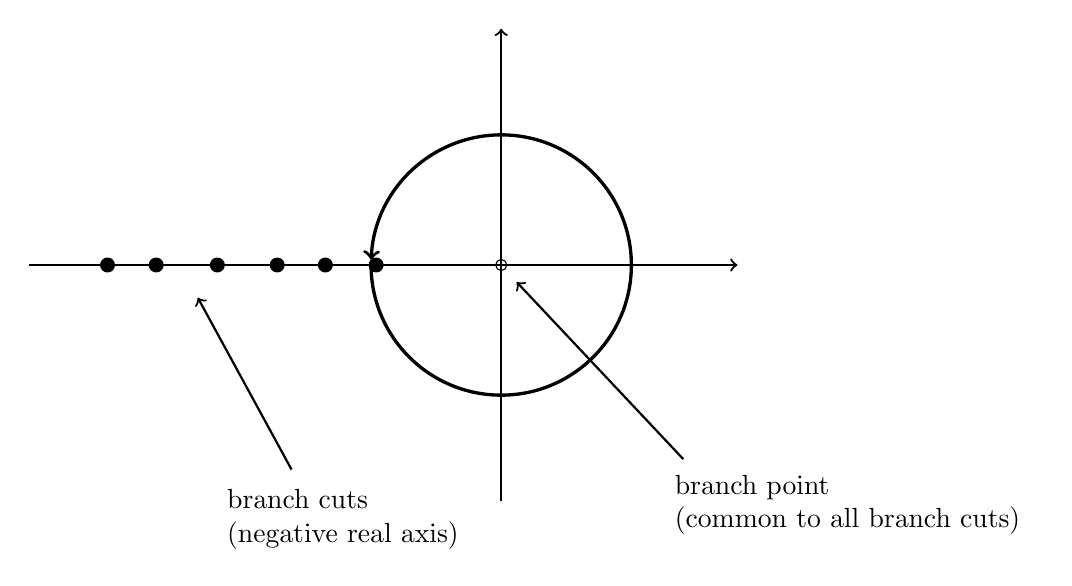
\begin{tikzpicture}
		\draw [->,line width=0.8pt] (-6,0) -- (3,0);
		\draw [->,line width=0.8pt] (0,-3) -- (0,3);
		\draw [shift={(0,0)},->,line width=1.2pt] (-180:1.6528925619834707) arc (-180:177.6721849109589:1.6528925619834707);
		\draw [->,line width=0.8pt] (-2.6629752066115677,-2.5973553719008198) -- (-3.853057851239666,-0.41553719008263945);
		\draw [->,line width=0.8pt] (2.3122314049586783,-2.4651239669421425) -- (0.19652892561983615,-0.21719008264462314);
		\draw (2.080826446280993,-2.5477685950413167) node[anchor=north west] {\parbox{4.570247933884296 cm}{branch point\\(common to all branch cuts)}};
		\draw (-3.6051239669421467,-2.7295867768594984) node[anchor=north west] {\parbox{3.6446280991735533 cm}{branch cuts \\ (negative real axis)}};
		\begin{scriptsize}
			\draw [color=black] (0,0) circle (2pt);
			\draw [fill=black] (-5,0) circle (2.5pt);
			\draw [fill=black] (-4.381983471074378,0) circle (2.5pt);
			\draw [fill=black] (-3.6051239669421467,0) circle (2.5pt);
			\draw [fill=black] (-2.84479338842975,0) circle (2.5pt);
			\draw [fill=black] (-2.233223140495866,0) circle (2.5pt);
			\draw [fill=black] (-1.588595041322312,0) circle (2.5pt);
		\end{scriptsize}
	\end{tikzpicture}
\end{center}
\begin{example}
	$$\Log_{-\frac{\pi}{2}} \ln |z| + i\Arg_{-\frac{\pi}{2}}(z)$$
	\begin{center}
		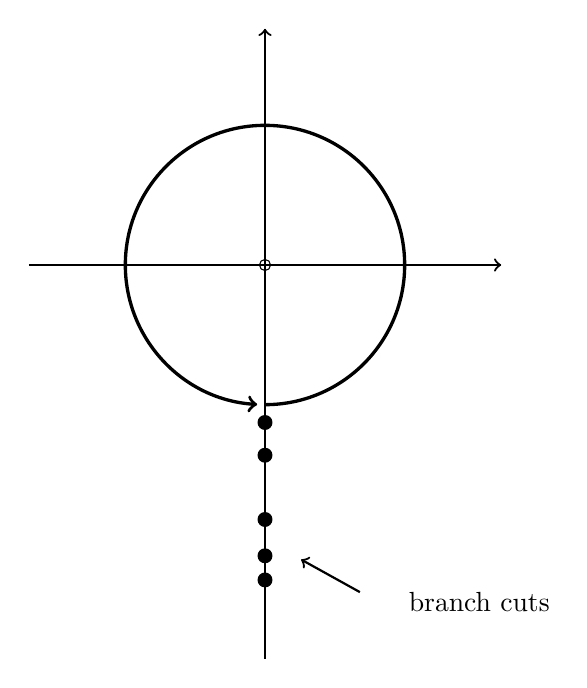
\begin{tikzpicture}
			\draw [->,line width=0.8pt] (-3,0) -- (3,0);
			\draw [->,line width=0.8pt] (0,-5) -- (0,3);
			\draw [shift={(0,0)},->,line width=1.2pt] (-90:1.7738359201773826) arc (-90:266.7698642896959:1.7738359201773826);
			\draw [->,line width=0.8pt] (1.2050433380366845,-4.154259221931055) -- (0.45841564200766105,-3.7405281193307647);
			\draw (1.7017173956863516,-4.030090707518638) node[anchor=north west] {branch cuts};
			\begin{scriptsize}
				\draw [fill=black] (0,-2) circle (2.5pt);
				\draw [color=black] (0,0) circle (2pt);
				\draw [fill=black] (0,-2.4159000201572205) circle (2.5pt);
				\draw [fill=black] (0,-3.231864543438816) circle (2.5pt);
				\draw [fill=black] (0,-3.693061882684935) circle (2.5pt);
				\draw [fill=black] (0,-4) circle (2.5pt);
			\end{scriptsize}
			\end{tikzpicture}
	\end{center}
\end{example}
\begin{example}
	Find a branch of $f(z) = \log(z+4)$ that is analytic at $z = -5$ and equals $7\pi i$ there. 

	\textbf{\underline{Solution}}: We want $\Log_{\tau}(-5+4) = \Log_{\tau}(-1) = 7\pi i$ for some $\tau$.

	So, $\ln|-1| + i\Arg_{\tau}(-1) = 7\pi i$ for some $k$, i.e. $$0 + i\underbrace{(\pi + 2k\pi)}_{\in (\tau, \tau + 2\pi]} = 7\pi i \;\;\text{ for some } k$$ 
	Hence, $k = 3$. We can choose $\tau = 6\pi$ so that $7\pi \in (6\pi, 8\pi]$. 

	The final answer would be $F(z) = \Log_{6\pi}(z+4)$
	\begin{center}
		\begin{tikzpicture}
			\draw [->,line width=0.8pt] (-8,0) -- (7,0);
			\draw [->,line width=0.8pt] (0,-3) -- (0,3);
			\draw [shift={(-5,0)},->,line width=1.2pt] (2.109283615747696:1.9965967101531474) arc (2.109283615747696:359.6393995753092:1.9965967101531474);
			\begin{scriptsize}
				\draw [color=black] (-5,0) circle (2.5pt);
				\draw [color=black] (-1.2227412365286425,-0.02377311401021034) circle (2.5pt);
				\draw [color=black] (-4,0) circle (2.5pt);
				\draw [color=black] (-2,0) circle (2.5pt);
				\draw [color=black] (0,0) circle (2.5pt);
				\draw [color=black] (1,0) circle (2.5pt);
				\draw [color=black] (2,0) circle (2.5pt);
				\draw [color=black] (3,0) circle (2.5pt);
				\draw [color=black] (4,0) circle (2.5pt);
				\draw [color=black] (5,0) circle (2.5pt);
			\end{scriptsize}
		\draw (-5,-0.5) node[anchor=north west] {\large -4};
		\end{tikzpicture}
	\end{center}
\end{example}
\begin{example}
	Where is $f(z) = \Log(z^2+1)$ analytic? 

	\textbf{\underline{Solution}}: We need $z^2+1 \neq 0$ and not equal to negative real number. 

	So, $z^2 +1 = (x+yi)^2+1 = (x^2-y^2+1) + i(2xy)$. 

	$z^2+1 = 0$ when $\begin{dcases}
		x = 0 \text{ and } y = \pm 1\\
		\text{or}\\
		y = 0 \text{ and } x^2+1 = 0 \text{ This is impossible for } x \in \mathbb{R}
	\end{dcases}$

	Hence, $z = \pm i$ here. 

	$z^2+1 < 0$ (real) when $\begin{dcases}
		x = 0 \text{ and } 1-y^2 < 0 & \Rightarrow y^2 > 1 \Rightarrow y > 1 \text{ or } y < -1\\
		\text{or}\\
		y = 0 \text{ and } 1+x^2 < 0 & \text{ Impossible}
	\end{dcases}$

	Hence, $z = iy$ where $|y| > 1$. 
	
	For all other points, $$f'(z) = \dfrac{2z}{z^2+1}$$
	\begin{center}
		\begin{tikzpicture}[scale=0.5]
			\draw (0.5,1) node[anchor=west] {$i$};
			\draw (0.5,-1) node[anchor=west] {$-i$};
			\draw [->,line width=0.8pt] (-3,0) -- (3,0);
			\draw [->,line width=0.8pt] (0,-5) -- (0,5);
			\draw [color=black] (0,-2) circle (2.5pt);
			\draw [color=black] (0,1) circle (2pt);
			\draw [color=black] (0,-1) circle (2pt);
			\draw [color=black] (0,-2) circle (2.5pt);
			\draw [color=black] (0,-3) circle (2.5pt);
			\draw [color=black] (0,-3.6) circle (2.5pt);
			\draw [color=black] (0,-4) circle (2.5pt);
			\draw [color=black] (0,2) circle (2.5pt);
			\draw [color=black] (0,3) circle (2.5pt);
			\draw [color=black] (0,3.6) circle (2.5pt);
			\draw [color=black] (0,4) circle (2.5pt);
		\end{tikzpicture}
	\end{center}
\end{example}

Here is another way to solve the above problem. $$\Log(z^2+1) = \Log\bigg((z+i)(z-i)\bigg) = \Log_{\tau_1}(z+i) + \Log_{\tau_2}(z-i)$$ for some $\tau_1, \tau_2$

Some possibilities are: \begin{itemize}
	\item $\tau_1 = \dfrac{-\pi}{2}$, $\tau_2 = \dfrac{-3\pi}{2}$
	\item $\tau_1 = \dfrac{3\pi}{2}$, $\tau_2 = \dfrac{-7\pi}{2}$
	\item $\cdots$
	\begin{center}
		\begin{tikzpicture}[scale=0.5]
			\draw [->,line width=0.8pt] (-3,0) -- (3,0);
			\draw [->,line width=0.8pt] (0,-5) -- (0,5);
			\draw [color=black] (0,-2) circle (2.5pt);
			\draw [color=black] (0,1) circle (2pt);
			\draw [color=black] (0,-1) circle (2pt);
			\draw [color=black] (0,-2) circle (2.5pt);
			\draw [color=black] (0,-3) circle (2.5pt);
			\draw [color=black] (0,-3.6) circle (2.5pt);
			\draw [color=black] (0,-4) circle (2.5pt);
			\draw [color=black] (0,2) circle (2.5pt);
			\draw [color=black] (0,3) circle (2.5pt);
			\draw [color=black] (0,3.6) circle (2.5pt);
			\draw [color=black] (0,4) circle (2.5pt);
		\end{tikzpicture}
	\end{center}
\end{itemize}

Finally, note that $$\Log z = \ln |z| + i \Arg z$$ $\Log z$ is analytic, so $\ln |z|$ and $\Arg z$ are harmonic. 

Level curves of $\ln |z| = k$ and $\Arg z = k$ are circles and rays. This would be particularly useful when we deal with temperature problems later. 
\begin{center}
	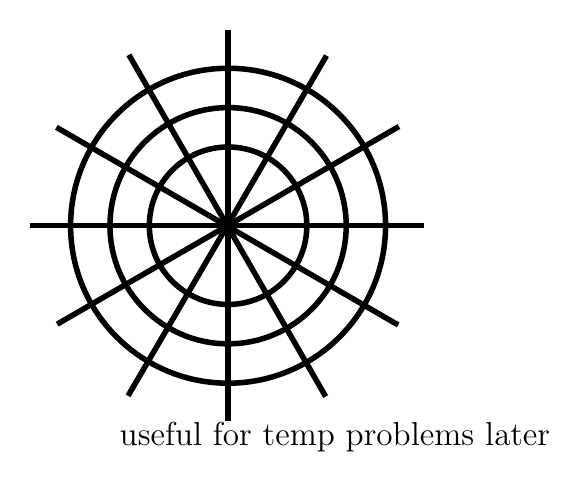
\begin{tikzpicture}[scale=0.5]
		\draw [line width=2pt] (0,0) circle (2.cm);
		\draw [line width=2pt] (0,0) circle (3cm);
		\draw [line width=2pt] (0,0) circle (4cm);
		\draw [line width=2pt] (-2.52,4.34)-- (2.48,-4.34);
		\draw [line width=2pt] (0,-4.96)-- (0,4.96);
		\draw [line width=2pt] (-4.36,2.5)-- (4.32,-2.52);
		\draw [line width=2pt] (-2.54,-4.32)-- (2.5,4.32);
		\draw [line width=2pt] (-5.02,0)-- (4.98,0);
		\draw [line width=2pt] (-4.34,-2.5)-- (4.34,2.52);
		\draw (-3,-6) node[anchor=south west] {\large useful for temp problems later};
	\end{tikzpicture}
\end{center}

\subsection{Complex Powers and Inverse Trigonometric Functions}
\begin{definition}
	\underline{\textbf{Complex Powers}}: We define $$z^\alpha = e^{\alpha \log z} \;\;\; \text{ for } \alpha \in \mathbb{C}, z \neq 0$$ 
\end{definition}
\begin{example}
	\begin{enumerate}
		\item \begin{align*}
			4^{1/2} &= e^{\frac{1}{2}\log 4}\\
			&=e^{\frac{1}{2}(\ln |4| + i \arg (4))}\\
			&=e^{\frac{1}{2}\ln 4 + i \frac{1}{2}(0+2\pi k)}\\
			&=e^{\frac{1}{2}2\ln 2 + i\pi k}\\
			&= e^{\ln 2} e^{i \pi k}\\
			&= 2 \cdot (\pm 1)\\
			&= \pm 2
		\end{align*}
		\item \begin{align*}
			(1+i)^3 &= e^{3 \log (1+i)}\\
			&=e^{3\big(\ln \sqrt{2} + i\arg (1+i)\big)}\\
			&=e^{\frac{3}{2}\ln 2}e^{i 3\big(\frac{\pi}{4}+ 2k\pi\big)}\\
			&=(e^{\ln 2})^{\frac{3}{2}} \cdot \bigg(\cos \dfrac{3\pi}{4} + i \sin \dfrac{3\pi}{4}\bigg)\\
			&=2^{\frac{3}{2}} \cdot \bigg(\dfrac{-1}{\sqrt{2}} + i\dfrac{1}{\sqrt{2}} \bigg)\\
			&=-2+2i
		\end{align*}
		\item \begin{align*}
			i^i &= e^{i \ln |i| + i \arg i}\\
			&=e^{i\big(0 + i (\frac{\pi}{2}+2k\pi)\big)}\\
			&=e^{-\big(\frac{\pi}{2}+2\pi k\big)}\\
			&= \cdots , e^{\frac{-5\pi}{2}}, e^{\frac{-\pi}{2}}, e^{\frac{3\pi}{2}}, \cdots
		\end{align*}
	\end{enumerate}
\end{example}
If we want a single value, take the principal branch to be $e^{\alpha \Log z}$, which is analytic everywhere $\Log z$ is, and $$\dfrac{d}{dz} z^{\alpha} = \dfrac{d}{dz} e^{\alpha \Log z} = e^{\alpha \Log z} \cdot \dfrac{\alpha}{z} = z^\alpha \cdot \dfrac{\alpha}{z} = \alpha z^{\alpha}$$
as expected.
\begin{definition}
	\underline{\textbf{Inverse Trigonometric Functions}}: First, we see that $w = \sin^{-1}z$ means $z = \sin w$, etc. Also, we've accepted multivalued functions. 

	In $\mathbb{R}$, the inverse hyperbolic function can be expressed in terms of logs: \begin{align*}
		y = \sinh x &= \dfrac{1}{2}(e^x - e^{-x})\\
		e^x - 2y -e^{-x} &= 0\\
		(e^x)^2 - 2y(e^x) -1 &= 0 \;\;\;\text{ note that this is a quadratic equation for }e^x\\
		e^x = \dfrac{2y \pm \sqrt{4y^2+4}}{2} &= y \pm \sqrt{y^2+1} \text{ we take the plus sign since } e^x > 0
	\end{align*}
	So, $x = \ln (y + \sqrt{y^2+1}) = \sinh^{-1}y$. 

	In $\mathbb{C}$, we define $\sinh^{-1}z = \log(z + \sqrt{z^2+1})$. 

	Similarly, $\sin^{-1}z = -i \log (iz + (1-z^2)^{\frac{1}{2}})$. Note that for this definition, it involves two sets of branches, one with $\log$, and the other one with $(1-z^2)^{\frac{1}{2}}$
\end{definition}
\section{Complex Integration}
\subsection{Contours}
How to integrate in $\mathbb{C}$? 

Complex values functions of a real variable are easy to integrate: $$\int_a^b \bigg(u(t)+iv(t)\bigg)dt = \int_a^b u(t)dt + i \int_a^b v(t)dt$$
\begin{example}
	\begin{enumerate}
		\item $$\int_0^1(t+i)^2 dt \int_0^1 \bigg((t^2-1)+i(2t)\bigg)dt = \dfrac{-2}{3}+2i$$
		\item We can use a special trick (instead of using integration by parts twice). 
		\begin{align*}
			\int_0^\pi e^{2\pi}\cos x dx &= \int_0^\pi e^2x(\Re(e^{ix}))dx\\
			&=\Re \bigg(\int_0^\pi e^{(2+i)\pi}\bigg)\\
			&=\Re \bigg(\left.\dfrac{e^{(2+i)}}{2+i} \right\vert_{0}^{\pi} \bigg)\\
			&=\Re \bigg(\left.\dfrac{e^{2x}(\cos x + i\sin x)}{2+i} \cdot \dfrac{2-i}{2-i}\right\vert_{0}^{\pi}\bigg)\\
			&=\bigg[\left.\dfrac{2}{5}e^{2x}\cos x + \dfrac{1}{5}e^{2x}\sin x \bigg]\right\vert_{0}^{\pi}\\
			&=-\dfrac{2}{5}e^{-2\pi} + \dfrac{2}{5}
		\end{align*}
	\end{enumerate}
\end{example}
What about integrating a function of a complex variable? 

We will replace the intervals with paths.
\begin{definition}
	Let $z(t) = x(t) + iy(t)$ on $t \in [a, b]$ be continuous. The range is a \underline{\textbf{curve}} $\mathcal{C}$, and is called a \textbf{\underline{smooth curve}} if $z'(t)$ is continuous and non-zero on $[a,b]$

	\begin{center}
		\begin{center}
			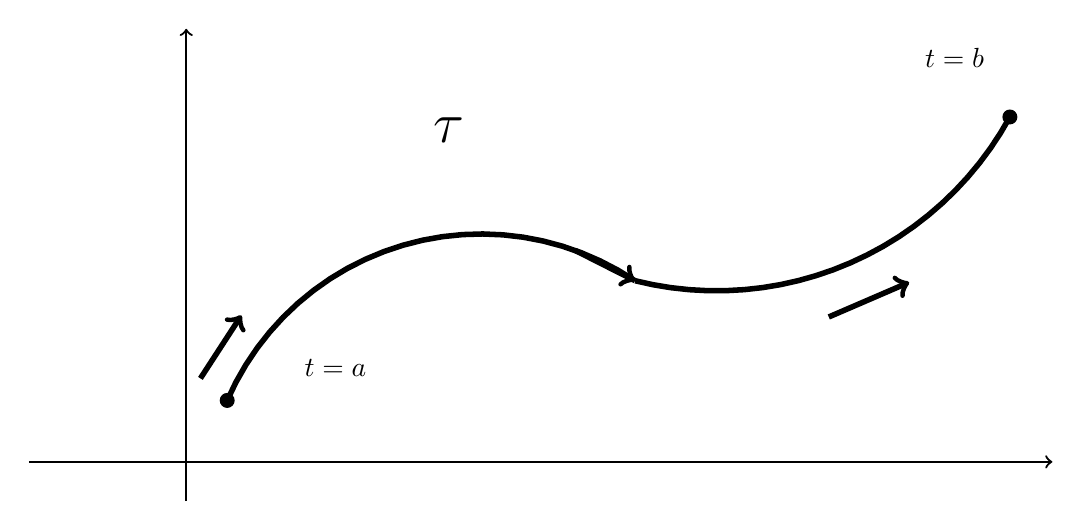
\begin{tikzpicture}
				\draw [->,line width=0.8pt] (-6,-0.5) -- (7,-0.5);
				\draw [->,line width=0.8pt] (-4,-1) -- (-4,5);
				\draw [shift={(-0.25584946236559125,-1.1211182795698924)},line width=2pt]  plot[domain=0.9807967459735268:2.73164434839709,variable=\t]({1*3.5154344145031557*cos(\t r)+0*3.5154344145031557*sin(\t r)},{0*3.5154344145031557*cos(\t r)+1*3.5154344145031557*sin(\t r)});
				\draw [shift={(2.7343127336705524,5.919553551792389)},line width=2pt]  plot[domain=4.466399761960735:5.782317247845397,variable=\t]({1*4.247413836338335*cos(\t r)+0*4.247413836338335*sin(\t r)},{0*4.247413836338335*cos(\t r)+1*4.247413836338335*sin(\t r)});
				\draw [->,line width=2pt] (0.9421669742181896,2.1838833452932853) -- (1.7,1.8);
				\draw [->,line width=2pt] (-3.82,0.56) -- (-3.3,1.36);
				\draw [->,line width=2pt] (4.16,1.34) -- (5.18,1.78);
				\draw (-2.62,0.92) node[anchor=north west] {$t=a$};
				\draw (5.26,4.88) node[anchor=north west] {$t=b$};
				\draw (-0.98,4) node[anchor=north west] {\huge $\tau$};
				\begin{scriptsize}
					\draw [fill=black] (-3.48,0.28) circle (2.5pt);
					\draw [fill=black] (6.46,3.88) circle (2.5pt);
				\end{scriptsize}
				\end{tikzpicture}
		\end{center}
	\end{center}

	A curve is called \textbf{\underline{simple}} if $z(t_1)\neq z(t_2)$ whenever $t_1 \neq t_2$ for $a < t_i < b$ (basically no self intersection)
	
	\begin{center}
		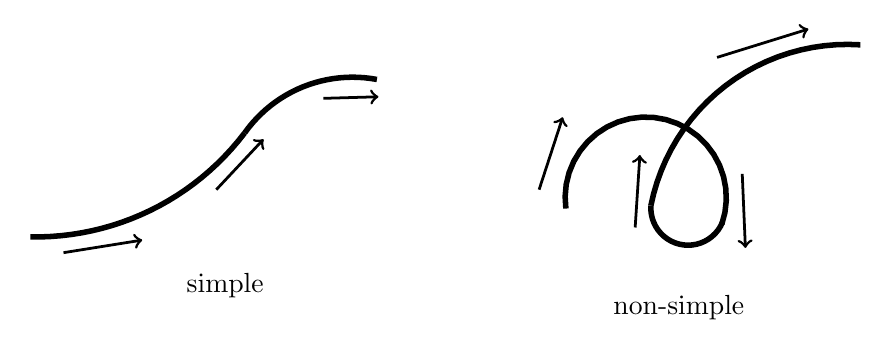
\begin{tikzpicture}
			\draw [shift={(-5.999587628865979,4.0579381443298965)},line width=2pt]  plot[domain=4.6942922471538715:5.634113397410818,variable=\t]({1*3.3384847925306693*cos(\t r)+0*3.3384847925306693*sin(\t r)},{0*3.3384847925306693*cos(\t r)+1*3.3384847925306693*sin(\t r)});
			\draw [shift={(-1.9696,1.0696)},line width=2pt]  plot[domain=1.3853605779174:2.5254415053168207,variable=\t]({1*1.6791879942400734*cos(\t r)+0*1.6791879942400734*sin(\t r)},{0*1.6791879942400734*cos(\t r)+1*1.6791879942400734*sin(\t r)});
			\draw (-4.2,0.38) node[anchor=north west] {simple};
			\draw (1.22,0.1) node[anchor=north west] {non-simple};
			\draw [shift={(1.7541468126207345,1.2190534449452672)},line width=2pt]  plot[domain=-0.3376013374048332:3.2778566866789682,variable=\t]({1*1.0236354908364311*cos(\t r)+0*1.0236354908364311*sin(\t r)},{0*1.0236354908364311*cos(\t r)+1*1.0236354908364311*sin(\t r)});
			\draw [shift={(2.292154717838775,1.0881031452258503)},line width=2pt]  plot[domain=3.074139205941243:5.883297847980803,variable=\t]({1*0.4732309023319334*cos(\t r)+0*0.4732309023319334*sin(\t r)},{0*0.4732309023319334*cos(\t r)+1*0.4732309023319334*sin(\t r)});
			\draw [shift={(4.315807275047862,0.6198787492022976)},line width=2pt]  plot[domain=1.5062464102482258:2.9438273487333233,variable=\t]({1*2.545422404961757*cos(\t r)+0*2.545422404961757*sin(\t r)},{0*2.545422404961757*cos(\t r)+1*2.545422404961757*sin(\t r)});
			\draw [->,line width=1pt] (0.4,1.32) -- (0.7,2.24);
			\draw [->,line width=1pt] (2.98,1.52) -- (3.02,0.58);
			\draw [->,line width=1pt] (2.66,3) -- (3.82,3.36);
			\draw [->,line width=1pt] (1.62,0.84) -- (1.68,1.76);
			\draw [->,line width=1pt] (-5.64,0.52) -- (-4.64,0.68);
			\draw [->,line width=1pt] (-3.7,1.32) -- (-3.1,1.96);
			\draw [->,line width=1pt] (-2.34,2.48) -- (-1.64,2.5);
		\end{tikzpicture}
	\end{center}

	If $z(a) = z(b)$, then the curve is called a \underline{\textbf{closed}} curve. 
	\begin{center}
		\begin{tikzpicture}[line cap=round,line join=round,>=triangle 45,x=1cm,y=1cm, scale=0.5]
			\clip(-8.94,-5.24) rectangle (8.9,5.24);
			\draw (-5.24,-0.1) node[anchor=north west] {simple closed curve};
			\draw [rotate around={-0.5256346064576136:(-3.44,2.18)},line width=2pt] (-3.44,2.18) ellipse (2.561498385867353cm and 1.3447951445484385cm);
			\draw [->,line width=1pt] (-4.24,3.96) -- (-5.3,3.6);
			\draw [->,line width=1pt] (-1.84,0.66) -- (-0.82,1.26);
			\begin{scriptsize}
				\draw [fill=black] (-1.46,3.02) circle (2.5pt);
			\end{scriptsize}
		\end{tikzpicture}
	\end{center}
\end{definition}
\begin{definition}
	\underline{\textbf{Contour}}: a curve that is composed of finitely many smooth curves, joined end-to-end
	\begin{center}
		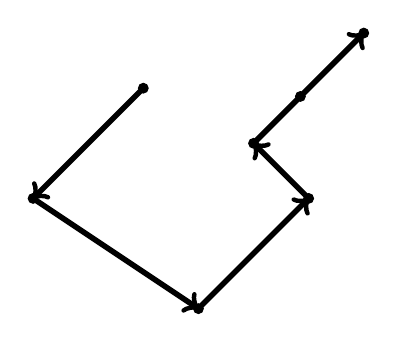
\begin{tikzpicture}[scale=0.7]
			\draw [->,line width=2pt] (-2,3) -- (-4,1);
			\draw [->,line width=2pt] (-4,1) -- (-1,-1);
			\draw [->,line width=2pt] (-1,-1) -- (1,1);
			\draw [->,line width=2pt] (1,1) -- (0,2);
			\draw [->,line width=2pt] (0,2) -- (2,4);
				\draw [fill=black] (-2,3) circle (2.5pt);
				\draw [fill=black] (-4,1) circle (2.5pt);
				\draw [fill=black] (-1,-1) circle (2.5pt);
				\draw [fill=black] (1,1) circle (2.5pt);
				\draw [fill=black] (0,2) circle (2.5pt);
				\draw [fill=black] (2,4) circle (2.5pt);
				\draw [fill=black] (0.85,2.85) circle (2.5pt);
		\end{tikzpicture}
	\end{center}
\end{definition}
\begin{definition}
	\textbf{\underline{Jordan Curve}}: a simple closed contour. 
	\begin{center}
		\begin{tikzpicture}[scale=0.7]
			\draw [line width=2pt] (-3,3)-- (-3,2);
			\draw [line width=2pt] (-3,1)-- (-3,0);
			\draw [line width=2pt] (-3,0)-- (-1,0);
			\draw [line width=2pt] (0,0)-- (2,0);
			\draw [line width=2pt] (-3,3)-- (-1,3);
			\draw [line width=2pt] (0,3)-- (2,3);
			\draw [->,line width=2pt] (-3,2) -- (-3,0.64);
			\draw [->,line width=2pt] (-1,0) -- (0.5,0);
			\draw [->,line width=2pt] (0,3) -- (-1.14,3);
			\draw [shift={(1.974305555555555,1.5)},line width=2pt]  plot[domain=-1.5536683722863849:1.5536683722863849,variable=\t]({1*1.5002200520174724*cos(\t r)+0*1.5002200520174724*sin(\t r)},{0*1.5002200520174724*cos(\t r)+1*1.5002200520174724*sin(\t r)});
			\draw [->,line width=1pt] (3.1,0.04) -- (3.76,0.76);
		\end{tikzpicture}
	\end{center}
\end{definition}
\begin{definition}
	\underline{\textbf{Positively Oriented}}: means its interior lies to the \textbf{\underline{left}} as we follow the curve 
	\begin{center}
		\begin{tikzpicture}[scale=0.7]
			\draw [shift={(-3.6435961272475796,1.366182572614108)},line width=2pt]  plot[domain=-0.1888212477248068:3.7677517930624838,variable=\t]({1*1.2050138375096797*cos(\t r)+0*1.2050138375096797*sin(\t r)},{0*1.2050138375096797*cos(\t r)+1*1.2050138375096797*sin(\t r)});
			\draw [shift={(4.824778887303846,-0.5206419400855922)},line width=2pt]  plot[domain=2.9174621442108837:3.4291939100256186,variable=\t]({1*7.471662137040131*cos(\t r)+0*7.471662137040131*sin(\t r)},{0*7.471662137040131*cos(\t r)+1*7.471662137040131*sin(\t r)});
			\draw [shift={(-1.6738689866939613,-2.4575332650972364)},line width=2pt]  plot[domain=3.4089546984895436:5.468504620115656,variable=\t]({1*0.6906697012568346*cos(\t r)+0*0.6906697012568346*sin(\t r)},{0*0.6906697012568346*cos(\t r)+1*0.6906697012568346*sin(\t r)});
			\draw [shift={(-0.8529559748427671,-3.3321855345911944)},line width=2pt]  plot[domain=-1.505989538730427:2.3212525496456813,variable=\t]({1*0.5088827247571559*cos(\t r)+0*0.5088827247571559*sin(\t r)},{0*0.5088827247571559*cos(\t r)+1*0.5088827247571559*sin(\t r)});
			\draw [shift={(-5.662695492180313,0.6421803127874881)},line width=2pt]  plot[domain=-1.6065757282617978:0.01708835685192156,variable=\t]({1*1.0428477504724725*cos(\t r)+0*1.0428477504724725*sin(\t r)},{0*1.0428477504724725*cos(\t r)+1*1.0428477504724725*sin(\t r)});
			\draw [shift={(-5.904015080113101,-1.1005466540999058)},line width=2pt]  plot[domain=1.2874114365651281:4.105741421103375,variable=\t]({1*0.7296490714611567*cos(\t r)+0*0.7296490714611567*sin(\t r)},{0*0.7296490714611567*cos(\t r)+1*0.7296490714611567*sin(\t r)});
			\draw [shift={(2.164636519748135,11.968551803091001)},line width=2pt]  plot[domain=4.156857863606362:4.525786580780108,variable=\t]({1*16.087832833107946*cos(\t r)+0*16.087832833107946*sin(\t r)},{0*16.087832833107946*cos(\t r)+1*16.087832833107946*sin(\t r)});
			\draw [->,line width=1pt] (-2.18,-1.32) -- (-2.18,-0.38);
			\draw [->,line width=1pt] (-3.08,2.86) -- (-4.18,2.88);
			\draw [->,line width=1pt] (-5.26,2.08) -- (-5.32,1.2);
			\draw [->,line width=1pt] (-5.9,-0.06) -- (-7.06,-0.36);
			\draw [->,line width=1pt] (-6.38,-2.1) -- (-5.46,-2.78);
			\draw [->,line width=1pt] (-0.04,-4.04) -- (0.28,-3.04);
		\end{tikzpicture}
	\end{center}
\end{definition}

\begin{example}
	Parameterize this: 
	\begin{center}
		\begin{tikzpicture}
			\draw [->,line width=2pt] (-3,0) -- (6,0);
			\draw [->,line width=2pt] (1,-1) -- (1,4);
			\draw [line width=2pt] (-1,1)-- (3,1);
			\draw [line width=2pt] (3,1)-- (5,3);
			\draw [->,line width=1pt] (-1,1) -- (0,1);
			\draw [->,line width=1pt] (3,1) -- (4,2);
			\draw [->,line width=1pt] (0,1) -- (2.2,1);
			\draw (0.52,1.9) node[anchor=north west] {$i$};
			\draw (0.38,3.3) node[anchor=north west] {$2i$};
			\draw (-1.46,0.02) node[anchor=north west] {$-1$};
			\draw (2.82,0.02) node[anchor=north west] {$1$};
			\draw (4.84,0.02) node[anchor=north west] {$2$};
			\begin{scriptsize}
				\draw [fill=black] (-1,1) circle (2.5pt);
				\draw [fill=black] (3,1) circle (2.5pt);
				\draw [fill=black] (5,3) circle (2.5pt);
			\end{scriptsize}
		\end{tikzpicture}
	\end{center}

	\underline{\textbf{Solution}}: Line segment from $z_0$ to $z_1$ can be parameterized as: $z(t) = z_0 + (z_1 - z_0)t, t \in [0, 1]$. 
	
	For the first curve, \begin{align*}
		z_1(t) &= (-1+i) + (1+i-(-1+i))t\\
		&=-1+i+2t, \;\;\;\; t \in [0,1]
	\end{align*}
	For the second curve, \begin{align*}
		z_2(t) &= (1+i) + (2+2i-(1+i))t\\
		&=1+i+(1+i)t, \;\;\;\; t \in [0,1]
	\end{align*}
	Put everything together we get $$z(t) = \begin{dcases}
		-1+i+2t & t \in [0,1)\\
		1+i+(1+i)(t-1) & t \in [1,2]
	\end{dcases}$$
\end{example}
\begin{example}
	Let $\mathcal{C}$ be a unit circle centered at 0.
	\begin{center}
		\begin{tikzpicture}[scale=0.5]
			\draw [line width=2pt] (0,0) circle (3cm);
			\draw [->,line width=2pt] (-4,0) -- (4,0);
			\draw [->,line width=2pt] (0,-4) -- (0,4);
			\draw [->,line width=1pt] (2.88,2.36) -- (2.22,3.08);
			\draw [->,line width=1pt] (-1.72,3.06) -- (-2.66,2.44);
			\draw [->,line width=1pt] (-3.26,-1.12) -- (-2.76,-1.82);
			\draw [->,line width=1pt] (2.46,-2.56) -- (3.22,-1.58);
			\draw (3.4174,1.4174) node[anchor=north west] {$t=0$};
			\draw (3.3514,-0.1886) node[anchor=north west] {$t=2\pi$};
		\end{tikzpicture}
	\end{center}

	\textbf{\underline{Solution}}: $\mathcal{C}: z(t) = e^{it} \;\;\; t \in [0, 2\pi]$
\end{example}
\begin{example}
	Circle, radius $r_0$, centered at $z_0$? 

	\textbf{\underline{Solution}}: $\mathcal{C}: z(t) = z_0 + r_0e^{it} \;\;\; t \in [0, 2\pi]$
\end{example}
\begin{example}
	Parameterize $y = f(x), x\in [a,b]$

	\textbf{\underline{Solution}}: just let $x(t) = t$, $$z(t) = x(t)+ iy(t) = t + if(t), \;\;\; t \in [a,b]$$
	For example, $y = x^2$ will be parameterized as $z(t) = t + it^2$
\end{example}
\begin{definition}
	\label{defn_Arclength}
	\underline{\textbf{Arclength}}: We define the arclength as follows: 
	\begin{center}
		\begin{tikzpicture}
			\draw [shift={(-5.767313432835821,0.2476119402985072)},line width=2pt]  plot[domain=0.7686526640717644:2.901124440109067,variable=\t]({1*2.3194243549602365*cos(\t r)+0*2.3194243549602365*sin(\t r)},{0*2.3194243549602365*cos(\t r)+1*2.3194243549602365*sin(\t r)});
			\draw [shift={(0.31600561272216865,5.379672591206732)},line width=2pt]  plot[domain=3.814517728837391:4.5170648131457805,variable=\t]({1*5.647052392256123*cos(\t r)+0*5.647052392256123*sin(\t r)},{0*5.647052392256123*cos(\t r)+1*5.647052392256123*sin(\t r)});
			\draw [->,line width=1pt] (-7.7,2.16) -- (-6.9,2.92);
			\draw [->,line width=1pt] (-5.52,2.9) -- (-4.62,2.62);
			\draw [->,line width=1pt] (0.84,0.82) -- (1.4,1.58);
			\draw [->,line width=1pt] (-2.22,1.12) -- (-1.32,0.72);
			\draw [shift={(-0.4598988439306359,2.4977745664739888)},line width=2pt]  plot[domain=4.592526772792368:6.0426280107639405,variable=\t]({1*2.676981583110527*cos(\t r)+0*2.676981583110527*sin(\t r)},{0*2.676981583110527*cos(\t r)+1*2.676981583110527*sin(\t r)});
			\draw [line width=2pt] (-4.1,1.86)-- (-4.1,0.78);
			\draw [line width=2pt] (-4.1,0.78)-- (-2.96,0.78);
			\draw [<->,line width=1pt] (-3.84,2.04) -- (-2.78,1);
			\draw (-9.32,1.4) node[anchor=north west] {$t=a$};
			\draw (2.66,2.24) node[anchor=north west] {$t=b$};
			\draw (-3.86,0.7) node[anchor=north west] {$\Delta{x}$};
			\draw (-5,1.7) node[anchor=north west] {$\Delta{y}$};
			\draw (-3.24,2) node[anchor=north west] {$\Delta s$};
			\draw (-0.02,2.44) node[anchor=north west] {$\Gamma$};
			\begin{scriptsize}
				\draw [fill=black] (-8.02,0.8) circle (2.5pt);
				\draw [fill=black] (-6.58,2.42) circle (2.5pt);
				\draw [fill=black] (-4.1,1.86) circle (2.5pt);
				\draw [fill=black] (-2.96,0.78) circle (2.5pt);
				\draw [fill=black] (0.1,-0.12) circle (2.5pt);
				\draw [fill=black] (2.14,1.86) circle (2.5pt);
				\draw [fill=black] (-4.1,0.78) circle (2.5pt);
			\end{scriptsize}
		\end{tikzpicture}
	\end{center}
	
	Partition the curve \begin{align*}
		\Delta s &\approx \sqrt{\Delta x^2 + \Delta y^2}\\
		&= \sqrt{\bigg(\dfrac{\Delta x}{\Delta t}\bigg)^2 + \bigg(\dfrac{\Delta y}{\Delta t}\bigg)^2} \Delta t
	\end{align*}
	Sum all pieces and let $\Delta t \rightarrow 0$ (Performing a Riemann Sum there): 
	\begin{align*}
		L = \int_R ds &= \int_a^b \sqrt{\bigg(\dfrac{dx}{dt}\bigg)^2+\bigg(\dfrac{dy}{dt}\bigg)^2} dt\\
		&=\int_a^b \left|\dfrac{dz}{dt}\right| dt \;\;\text{ we use modulus here}
	\end{align*}
	The physical interpretation could be: $\text{total\_distance} = \int_a^b (\text{speed})\;dt$
\end{definition}
Now we are ready to integrate $f(z)$ along a curve. 

\subsection{Contour Integrals}
Partition curve $\mathcal{C}$ as shown. 
\begin{center}
	\begin{tikzpicture}
		\draw [shift={(-1.3292025542718235,-2.0305186851097754)},line width=2pt]  plot[domain=0.9884887019921226:2.56851289758992,variable=\t]({1*2.4169396950685256*cos(\t r)+0*2.4169396950685256*sin(\t r)},{0*2.4169396950685256*cos(\t r)+1*2.4169396950685256*sin(\t r)});
		\draw [shift={(0.9843621078196576,2.6220842448625032)},line width=2pt]  plot[domain=4.354744569311382:6.175547368193567,variable=\t]({1*2.8119114700126486*cos(\t r)+0*2.8119114700126486*sin(\t r)},{0*2.8119114700126486*cos(\t r)+1*2.8119114700126486*sin(\t r)});
		\draw [line width=2pt] (-0.3171126950022274,0.16430969231785086) circle (0.7475440004282073cm);
		\draw [line width=1pt] (-1.0362019819326107,0.3685953501554997)-- (-1.280826446280993,3.343471074380167);
		\draw [line width=1pt] (0.3731798093470926,-0.12260195090241277)-- (1.7439669421487551,3.1781818181818196);
		\draw [line width=2pt] (0.2542208052260085,3.6753316447269215) circle (1.570509949828422cm);
		\draw [line width=1pt] (-0.7699388865579713,3.6876383020935997)-- (1.377247260628173,3.8261664406217384);
		\draw [->,line width=1pt] (4.113177996558903,0.6746512891065873) -- (4.39023427361518,1.6097162241715222);
		\draw [->,line width=1pt] (-2.6747007913198737,-0.9876863732310747) -- (-2.0513241679432515,-0.32967771522241673);
		\draw [->,line width=1pt] (-0.8738349904540759,-0.6586820442267457) -- (0.13049401387492687,-0.8664742520189535);
		\draw [->,line width=1pt] (1.6543035376844482,-0.8664742520189535) -- (2.6932645766454857,-0.29504568059038205);
		\draw (1.5677234511043618,5.505820120275418) node[anchor=north west] {$\Delta z_k = z_k-z_{k-1}$};
		\draw (1.7928316762125867,1.2807118951671934) node[anchor=north west] {$\mathcal{C}$};
		\draw (-0.9950471116661969,3.4452140596693575) node[anchor=north west] {$z_{k-1}$};
		\draw (1.1867710701519816,3.5144781289334266) node[anchor=north west] {$z_k$};
		\draw (0.061229944610857734,4.657335271790569) node[anchor=north west] {$z^x_{k}$};
		\begin{scriptsize}
			\draw [fill=black] (-3.36,-0.72) circle (2.5pt);
			\draw [fill=black] (-2.26,0.2) circle (2.5pt);
			\draw [fill=black] (0,-0.011900826446279563) circle (2.5pt);
			\draw [fill=black] (2,0) circle (2.5pt);
			\draw [fill=black] (3.78,2.32) circle (2.5pt);
			\draw [fill=black] (-0.6423235200560911,0.2867630590794805) circle (2.5pt);
			\draw [fill=black] (0.8892571571178356,-0.18821843697457918) circle (2.5pt);
			\draw [fill=black] (2.7228242861993244,0.41197217314936996) circle (2.5pt);
			\draw [fill=black] (3.3765662116567574,1.1441784153951344) circle (2.5pt);
			\draw [fill=black] (3.700053202848346,1.8927914425049202) circle (2.5pt);
			\draw [fill=black] (-2.870898651711336,-0.16912924903313487) circle (2.5pt);
			\draw [fill=black] (-1.4689435447205046,0.382377903056895) circle (2.5pt);
			\draw [fill=black] (-0.7699388865579713,3.6876383020935997) circle (2.5pt);
			\draw [fill=black] (1.377247260628173,3.8261664406217384) circle (2.5pt);
			\draw [fill=black] (0.2725032999256636,3.7548926367054474) circle (2.5pt);
		\end{scriptsize}
	\end{tikzpicture}
\end{center}

Sum, and let $\max |\Delta z_k| \rightarrow 0$: $$\int_{\mathcal{C}}f(z)dz = \lim_{\max |\Delta z_k| \rightarrow 0} \sum_{k} f(z_k^*)\Delta z_k$$
See the text for more detail.

If $\mathcal{C}$ is a single point, define $\int_{\mathcal{C}}f(z)dz = 0$. 

How to calculate? 
\begin{definition}
	Assume $\mathcal{C}$ has a parameterization. Call it $z(t), t \in [a,b]$. Then: \begin{align*}
		\int_{\mathcal{C}} f(z)dz &= \lim_{\max |\Delta z_k| \rightarrow 0} \sum_{k} f(z_k^*) \dfrac{\overbrace{z(t_k)}^{z_k} - \overbrace{z(t_{k-1})}^{z_{k-1}}}{\Delta t_k} \Delta t_k\\
		&= \int_{a}^{b} f(z)z'(t) dt
	\end{align*}
\end{definition}
\begin{proposition}
	Properties: \begin{itemize}
		\item $\displaystyle\int_{\mathcal{C}} \bigg(f(z) +g(z) \bigg)dz = \int_{\mathcal{C}} f(z)dz + \int_{\mathcal{C}} g(z)dz$
		\item $\displaystyle\int_{\mathcal{C}} kf(z)dz = k\int_{\mathcal{C}} f(z)dz$
		\item $\displaystyle\int_{-\mathcal{C}} f(z)dz = -\int_{\mathcal{C}} f(z)dz$. Here $-\mathcal{C}$ means $\mathcal{C}$ traversed in the opposite direction
		\item $\displaystyle\int_{\mathcal{C}_1 + \mathcal{C}_2} f(z)dz = \int_{\mathcal{C}_1} f(z)dz + \int_{\mathcal{C}_2} f(z)dz$. Here it means that we traverse $\mathcal{C}_1$ then traverse $\mathcal{C}_2$. 
		\begin{center}
			\begin{tikzpicture}
				\draw [shift={(-4.873716704521987,-4.1312925872393205)},line width=2pt]  plot[domain=1.4439239249118083:2.378792027289586,variable=\t]({1*4.85027675018997*cos(\t r)+0*4.85027675018997*sin(\t r)},{0*4.85027675018997*cos(\t r)+1*4.85027675018997*sin(\t r)});
				\draw [shift={(-1.4464101935800047,5.680901739769662)},line width=2pt]  plot[domain=4.199911030102511:5.195671924244747,variable=\t]({1*5.738057668725693*cos(\t r)+0*5.738057668725693*sin(\t r)},{0*5.738057668725693*cos(\t r)+1*5.738057668725693*sin(\t r)});
				\draw [->,line width=2pt] (-8.38,-0.78) -- (-7.488743267982007,-0.04634208254139249);
				\draw [->,line width=2pt] (-4.26,0.68) -- (-3.1529910636478036,0.202499824654236);
				\draw (-6.36,0.08) node[anchor=north west] {$\mathcal{C}_1$};
				\draw (-0.9,-0.24) node[anchor=north west] {$\mathcal{C}_2$};
				\begin{scriptsize}
					\draw [fill=black] (-8.38,-0.78) circle (2.5pt);
					\draw [fill=black] (-4.26,0.68) circle (2.5pt);
					\draw [fill=black] (1.22,0.6) circle (2.5pt);
					\draw[color=black] (1.38,1.03) node {$E$};
				\end{scriptsize}
			\end{tikzpicture}
		\end{center}
	\end{itemize}
\end{proposition}

Is there a triangle inequality? i.e. $$\left| \int_{\mathcal{C}} f(z)dz \right| \leq_? \int_{\mathcal{C}} \left| f(z) \right| dz$$

No! LHS is real, but RHS is complex. ``$\leq$'' does NOT make any sense here. 

\begin{proposition}
	\underline{\textbf{The ``ML'' Inequality}}: If $f(z)$ is continuous on a contour $\mathcal{C}$, then $$\left| \int_{\mathcal{C}} f(z)dz \right| \leq ML$$
	where $M$ is an upper bound for $|f(z)|$ on $\mathcal{C}$ and $L$ is the length of $\mathcal{C}$. 
\end{proposition}
\begin{proof}
	Let $z(t)$, $t \in [a,b]$ be a parameterization of $\mathcal{C}$. Then \begin{align*}
		\left| \int_{\mathcal{C}} f(z)dz \right| &= \left| \int_{a}^b f(z(t))z'(t) dt\right|\\
		&\leq \int_{a}^b \bigg|f(z(t))z'(t)\bigg| dt \;\;\text{ by triangle inequality for integrals w.s.t. real variables}\\
		&= M \int_{a}^b \bigg| z'(t)\bigg| dt\\
		&= ML
	\end{align*}
	Second last step: since $|f(z)| \leq M$ on $\mathcal{C}$. 

	Last step: from last lecture. See Definition \ref{defn_Arclength}.
\end{proof}
\begin{example}
	Find an upper bound on $\left| \int_{\mathcal{C}} e^{\frac{1}{z}}\right|$
	\begin{center}
		\begin{tikzpicture}[scale=1.5]
			\draw (1.5534076199727505,1.04130100687539) node[anchor=north west] {$\mathcal{C}$ is unit circle, traversed \underline{once} in positive direction};
			\draw [->,line width=2pt] (-2,0) -- (2,0);
			\draw [->,line width=2pt] (0,-2) -- (0,2);
			\draw [line width=2pt] (0,0) circle (1cm);
			\draw [shift={(0,0.0278)},->,line width=2pt] (-150.13762460175298:1.0181929476078775) arc (-150.13762460175298:-116.67295733591709:1.0181929476078775);
			\draw [shift={(0,-0.0278)},->,line width=2pt] (20.65891618285383:1.0181929476078775) arc (20.65891618285383:58.11963965317466:1.0181929476078775);
		\end{tikzpicture}
	\end{center}
	\underline{\textbf{Solution}}: $M = ?$\begin{align*}
		\left| e^{\frac{1}{z}} \right| &= \left| e^{\frac{1}{x+iy}} \right|\\
		&=\left| e^{\frac{x-iy}{x^2+y^2}} \right|\\
		&=\left| e^{\frac{x}{x^2+y^2}} \cdot e^{-i \frac{y}{x^2+y^2}}\right|\\
		&\leq e^{\frac{x}{1}} \;\;\text{ since }x^2+y^2 = 1\\
		&\leq e^1 \;\; \text{ since } x \leq 1
	\end{align*}
	Clearly, $L = 2\pi$, so $\left| e^{\frac{1}{z}} \right| \leq e^1 \cdot 2\pi = 2\pi e$ by ML inequality. 
\end{example}
\begin{example}
	Evaluate $\int_{\mathcal{C}} \cos z dz$ where $\mathcal{C}$ is the line segment from 0 to 1+2i. 
	\begin{center}
		\begin{tikzpicture}[scale=1.5]
			\draw [->,line width=2pt] (-0.5,0) -- (2,0);
			\draw [->,line width=2pt] (0,-0.5) -- (0,2);
			\draw [line width=2pt] (0,0) -- (1,1);
			\draw [->,line width=2pt] (0,0) -- (0.5,0.5);
			\draw [fill=black] (1,1) circle (1pt);
			\draw [fill=black] (0,0) circle (1pt);
			\draw [fill=black] (1,1) node[anchor=north west] {$1+2i$};
		\end{tikzpicture}
	\end{center}
	\textbf{\underline{Solution}}: Parameterize $\mathcal{C}$ by $$z(t) = 0+(1+2i-0)t, \;\;\; t \in [0,1]$$
	Then $$\int_{\mathcal{C}} \cos z dx = \int_{0}^{1} \underbrace{\cos \bigg( (1+2i)t\bigg)}_{f(z(t))}\cdot \underbrace{(1+2i)}_{z'(t)} dt = \left. \sin \bigg( (1+2i)t\bigg) \right|_{0}^{1} = \sin(1+2i) - 0 = \sin(1+2i)$$
\end{example}
\begin{example}
	Evaluate $\int_{\mathcal{C}} \cos z dz$ where $\mathcal{C}$ is: 
	\begin{center}
		\begin{tikzpicture}[scale=1.5]
			\draw [->,line width=2pt] (-0.5,0) -- (2.5,0);
			\draw [->,line width=2pt] (0,-0.5) -- (0,3);
			\draw [line width=2pt] (0,0) -- (1,0);
			\draw [line width=2pt] (1,0) -- (1,2);
			\draw [->,line width=2pt] (0,0) -- (0.5,0);
			\draw [->,line width=2pt] (1,0) -- (1,1);
			\draw [fill=black] (1,2) circle (1pt);
			\draw [fill=black] (0,2) circle (1pt);
			\draw [fill=black] (0,0) circle (1pt);
			\draw [fill=black] (1,2) node[anchor=north west] {$1+2i$};
			\draw [fill=black] (1,0) node[anchor=north] {$1$};
			\draw [fill=black] (0,2) node[anchor=east] {$2i$};
		\end{tikzpicture}
	\end{center}
	\textbf{\underline{Solution}}: $\mathcal{C} = \mathcal{C}_1 \cup \mathcal{C}_2$ where $\begin{dcases}
		C_1: & z(t) = t, \;\; t\in [0,1)\\
		C_2: & z(t) = 1+(t-1)i, \;\; t \in [1,3]
	\end{dcases}$. So \begin{align*}
		\int_{\mathcal{C}} \cos z dx &= \int_{\mathcal{C}_1} \cos z dx + \int_{\mathcal{C}_2} \cos z dx\\
		&=\int_{0}^1 \cos t dt + \int_{1}^3 \cos (1+(t-1)i) i dt\\
		&= \left. \sin t \right|_0^1 + \left. \sin (1+(t-1)i) \right|_1^3\\
		&= \sin (1) + (\sin (1+2i) - \sin (1))\\
		&= \sin (1+2i)
	\end{align*}
	As before
\end{example}
\begin{example}
	Evaluate $\int_{\mathcal{C}} e^z dz$ where $\mathcal{C}$ is part of $y = x^2 + 1$ from $z = i$ to $z = 2+5i$. 

	\begin{center}
		\begin{tikzpicture}[scale=1.5]
			\draw[<->](2,0)--(0,0)--(0,3);
			\draw(0,0)--(-2,0);
			\draw[black,dashed,domain=-1:1] plot(\x,2*\x*\x + 1);
			\draw [fill=black] (0,1) circle (1pt) node[anchor=south west] {$i$};
			\draw [fill=black] (0.75,2.1) circle (1pt) node[anchor=south west] {$2+5i$};
			\draw [->,line width=1pt] (0.35,0.75) -- (0.75,1.2);
		\end{tikzpicture}
	\end{center}

	\textbf{\underline{Solution}}: Let $z(t) = \underbrace{t}_x + \underbrace{(t^2+1)}_y i, \;\; t \in [0,2]$. Then, \begin{align*}
		\int_{\mathcal{C}} e^z dz &= \int_{0}^{2} e^{z(t)} z'(t) dt\\
		&= \int_{0}^{2} e^{t^2+(t^2+1)i} (1+2ti) dt\\
		&= \left. e^{t^2+(t^2+1)i} \right |_0^2\\
		&= e^{2+5i} - e^i\\
		&= e^z \big|_i^{2+5i}
	\end{align*}
\end{example}
Does it always work that way? See the following example
\begin{example}
	Evaluate $\int_{\mathcal{C}} \overline{z} dz$ where \begin{enumerate}
		\item $\mathcal{C}$ is line segment from 0 to $1+i$
		\item $\mathcal{C}$ is the smallest arc of circle $x^2+(y-1)^2 = 1$ from 0 to $1+i$
	\end{enumerate}
	\begin{center}
		\begin{tikzpicture}[scale=0.8]
			\begin{axis}[
				axis lines = middle,
				xtick= \empty,
				ytick= \empty,
				]
				\addplot[
				ultra thick,
				domain=0:1, 
				samples=100, 
				color=black,
				] {x^2};
			\end{axis}
			\draw [line width=1.5pt] (0,0) -- (6.85,5.7);
			\draw [->,line width=1.5pt] (0,0) -- (2,1.644);
			\draw [->,line width=1.5pt] (0,0) -- (5,4.161);
			\draw [fill=black] (6.85,5.7) circle (2pt) node[anchor=south west] {$1+i$};
			\draw (6,3) node[anchor=south west] {$(b)$};
			\draw (3,4) node[anchor=south west] {$(a)$};
			\draw [->,line width=1pt] (3.35,0.75) -- (3.75,1.2);
		\end{tikzpicture}
	\end{center}

	\textbf{\underline{Solution}}: \begin{enumerate}
		\item parameterization: $z(t) = t(1+i), \;\; t \in [0,1]$
		
		\begin{align*}
			\int_{\mathcal{C}} \overline{z} dz &= \int_{0}^1 t(1-i)\cdot (1+i) dt\\
			&= \int_0^1 2t dt\\
			&=1
		\end{align*}
		\item parameterization: $z(t) = e^{it} + i, \;\; t \in [\dfrac{-\pi}{2},0]$. It's the unit circle, shifted up by 1 unit. 
		
		\begin{align*}
			\int_{\mathcal{C}} \overline{z} dz &= \int_{-\pi / 2}^0 (e^{-it} - i) (ie^{it}) dt\\
			&= \cdots\\
			&= 1+i(\frac{\pi}{2} - 1) dt\\
			&\neq 1
		\end{align*}
	\end{enumerate}
	So, the general answer is no. Different paths might yield different results. 
\end{example}
\subsection{Independence of Path}
\begin{theorem}
	\label{theorem_FTC}
	\underline{\textbf{Complex Extension of Fundamental Theorem of Calculus}}: 

	If $f(z)$ is continuous in a domain $D$ and has antiderivative $F(z)$ throughout $D$, then, for any contour $\mathcal{C}$ lying in $D$ with initial point $z_1$ and terminal point $z_2$, we have $$\int_{\mathcal{C}} f(z) dz = F(z_2) - F(z_1)$$
	\begin{center}
		\begin{tikzpicture}
			\draw [shift={(-3.21,-3.6625)},line width=2pt]  plot[domain=0.9950484961787569:2.2972019390677167,variable=\t]({1*3.508048781017732*cos(\t r)+0*3.508048781017732*sin(\t r)},{0*3.508048781017732*cos(\t r)+1*3.508048781017732*sin(\t r)});
			\draw [shift={(-0.10856502242152467,1.866681614349776)},line width=2pt]  plot[domain=4.28075213328399:5.906833913364336,variable=\t]({1*2.847883263024063*cos(\t r)+0*2.847883263024063*sin(\t r)},{0*2.847883263024063*cos(\t r)+1*2.847883263024063*sin(\t r)});
			\draw [->,line width=2pt] (-2.0079049224843537,-0.36684017613882736) -- (-0.9100552328849356,-0.8660921637635719);
			\draw (-6.12,-0.14) node[anchor=north west] {$(t=a)$};
			\draw (1.94,1.44) node[anchor=north west] {$(t=b)$};
				\draw [fill=black] (-5.54,-1.04) circle (2.5pt);
				\draw[color=black] (-5.3,-1.59) node {$z_1$};
				\draw [fill=black] (2.54,0.82) circle (2.5pt);
				\draw[color=black] (2.66,0.35) node {$z_2$};
		\end{tikzpicture}
	\end{center}
\end{theorem}
\begin{proof}
	First, suppose $\mathcal{C}$ is smooth, i.e. $z'(t) \neq 0$, continuous. 

	Parameterize by $z(t), t \in [a,b]$. Then, \begin{align*}
		\int_{\mathcal{C}} f(z) dz &= \int_a^b f(z(t))z'(t) dt\\
		&=\int_{\mathcal{C}} \dfrac{d}{dt} \bigg(F\big(z(t)\big)\bigg) dt \;\; \text{ by chain rule}\\
		&=F(z(t)) \bigg|_{t=a}^b\\
		&=F(z(b)) - F(z(a))\\
		&=F(z_2) - F(z_1)
	\end{align*}
	Next, if $\mathcal{C}$ is not smooth, it has a finite number of smooth pieces, since it's a contour. 

	\begin{center}
		\begin{tikzpicture}[scale=1.2]
			\draw [shift={(-5.0430841121495344,-1.5912550066755653)},line width=2pt]  plot[domain=1.5929506495087926:2.4511706862468396,variable=\t]({1*3.4721070512260996*cos(\t r)+0*3.4721070512260996*sin(\t r)},{0*3.4721070512260996*cos(\t r)+1*3.4721070512260996*sin(\t r)});
			\draw [shift={(-2.014512841169199,5.73484349993133)},line width=2pt]  plot[domain=4.178998516845949:5.08841755516068,variable=\t]({1*3.19830803131203*cos(\t r)+0*3.19830803131203*sin(\t r)},{0*3.19830803131203*cos(\t r)+1*3.19830803131203*sin(\t r)});
			\draw [line width=2pt] (-5.12,1.88)-- (-3.640710936855408,2.9808184425395896);
			\draw [line width=2pt] (1.1084839641747943,2.7638501475686668)-- (2.72,2.82);
			\draw [line width=2pt] (2.72,2.82)-- (3.165825552265748,0.5886224525435144);
			\draw [->,line width=2pt] (-7.72,0.62) -- (-7.18206513988621,1.1437564262359237);
			\draw [->,line width=2pt] (-5.12,1.88) -- (-4.4068018683208106,2.41072903470827);
			\draw [->,line width=2pt] (-3.640710936855408,2.9808184425395896) -- (-3.063056491325477,2.713299113881047);
			\draw [->,line width=2pt] (1.1084839641747943,2.7638501475686668) -- (1.9119854212326397,2.7918464487156527);
			\draw [->,line width=2pt] (2.72,2.82) -- (2.9321304741182845,1.7582771474778813);
			\draw [->,line width=2pt] (-6.7,1.46) -- (-5.943783764132144,1.7619923018438057);
			\draw [->,line width=2pt] (-2.54,2.58) -- (-1.8950418747273785,2.53876763235051);
				\draw [fill=black] (-7.72,0.62) circle (2.5pt);
				\draw[color=black] (-7.539631197482891,0.3479684520382659) node {$z_1=a_0$};
				\draw [fill=black] (-6.7,1.46) circle (2.5pt);
				\draw[color=black] (-6.5186748317030485,1.295999363119548) node {$a_1$};
				\draw [fill=black] (-5.12,1.88) circle (2.5pt);
				\draw[color=black] (-4.9288999192744365,1.675211727552061) node {$a_2$};
				\draw [fill=black] (-3.640710936855408,2.9808184425395896) circle (2.5pt);
				\draw[color=black] (-3.747507553157761,2.419051365477375) node {$a_3$};
				\draw [fill=black] (-2.54,2.58) circle (2.5pt);
				\draw[color=black] (-2.5952853689205098,2.127349546683134) node {$a_4$};
				\draw [fill=black] (-0.84,2.76) circle (2.5pt);
				\draw [fill=black] (1.1084839641747943,2.7638501475686668) circle (2.5pt);
				\draw [fill=black] (2.72,2.82) circle (2.5pt);
				\draw[color=black] (2.3198902777624473,2.3315408198391028) node {$a_{n-1}$};
		
				\draw [fill=black] (3.165825552265748,0.5886224525435144) circle (2.5pt);
				\draw[color=black] (2.8303684606523687,0.7709360892899149) node {$a_{n}$};
				\draw [fill=black] (-0.2624624641389859,2.761141197351578) circle (1.5pt);
				\draw [fill=black] (0.1441841960414415,2.7619447193095654) circle (1.5pt);
				\draw [fill=black] (0.6383878272097848,2.762921251292355) circle (1.5pt);
				\draw[color=black] (-7.5688013793623155,1.4272651815769564) node {$\mathcal{C}_1$};
				\draw[color=black] (-6.139462467270535,2.0106688191654376) node {$\mathcal{C}_2$};
				\draw[color=black] (-4.695538464239044,2.7690935480304635) node {$\mathcal{C}_3$};
				\draw[color=black] (-3.047423188051583,3.148305912462977) node {$\mathcal{C}_4$};
				\draw[color=black] (1.8385822767519502,3.2649866399806724) node {$\mathcal{C}_{n-1}$};
				\draw[color=black] (3.4721124619996986,2.112764455743422) node {$\mathcal{C}_{n}$};
		\end{tikzpicture}
	\end{center}

	Apply the result above to each piece: \begin{align*}
		\int_{\mathcal{C}} f(z) dz &= \int_{\mathcal{C}_1} f(z) dz + \cdots + \int_{\mathcal{C}_n} f(z) dz\\
		&=\bigg(F(a_1) - F(a_0)\bigg) + \bigg(F(a_2) - F(a_1)\bigg) + \cdots + \bigg(F(a_n) - F(a_{n-1})\bigg) \\
		&=F(a_n) - F(a_0)\\
		&= F(z_2) - F(z_1)
	\end{align*}
\end{proof}
\begin{example}
	Evaluate $\int_{\mathcal{C}}(1+z^2) dz$ where $\mathcal{C}$ is: 
	\begin{center}
		\begin{tikzpicture}[scale=0.7]
			\draw [->,line width=1pt] (-1,0) -- (6,0);
			\draw [->,line width=1pt] (0,-1) -- (0,6);
			\draw [fill=black] (0,0) circle (2pt);	
			\draw [fill=black] (4,2) circle (2pt) node[anchor=north west]{$4+2i$};
			\draw [fill=black] (2,-2) circle (2pt) node[anchor=north west]{$2-2i$};
			\draw [line width=2pt] (0,0) -- (2,-2);
			\draw [line width=2pt] (2,-2) -- (4,2);
			\draw [->,line width=2pt] (0,0) -- (1,-1);
			\draw [->,line width=2pt] (2,-2) -- (3,0);
		\end{tikzpicture}
	\end{center}

	\textbf{\underline{Solution}}: \begin{align*}
		\int_{\mathcal{C}}(1+z^2) dz &= \left. \left( z + \dfrac{z^3}{4}\right) \right|_{z=0}^{z=4+2i}\\
		&= \cdots\\
		&= \dfrac{28}{3} + \dfrac{94}{3}i
	\end{align*}
\end{example}
\begin{example}
	Evaluate $\int_{\mathcal{C}}e^z dz$ where $\mathcal{C}$ is: 
	
	\begin{center}
		\begin{tikzpicture}
			\draw [->,line width=1pt] (-2,0) -- (2,0);
			\draw [->,line width=1pt] (0,-2) -- (0,3);
			
			\draw [fill=black] (1,-1) circle (2pt)node[anchor=west]{$1-i$, staring point};
			\draw [fill=black] (0,2) circle (2pt) node[anchor=west]{$2i$};
			\draw [fill=black] (-1,-1) circle (2pt) node[anchor=north east]{$-1-i$};
			
			\draw [line width=2pt] (1,-1) -- (0,2);
			\draw [line width=2pt] (0,2) -- (-1,-1);
			\draw [line width=2pt] (-1,-1) -- (1,-1);
			\draw [->,line width=2pt] (1,-1) -- (0.3333,1);
			\draw [->,line width=2pt] (-1,-1) -- (0,-1);
			\draw [->,line width=2pt] (0,2) -- (-0.6667,0);
		\end{tikzpicture}
	\end{center}

	\textbf{\underline{Solution}}: \begin{align*}
		\int_{\mathcal{C}}(1+z^2) dz &= e^z \big|_{z=1-i}^{z=1-i}\\
		&= e^{1-i} - e^{1-i}\\
		&= 0
	\end{align*}
\end{example}
\begin{theorem}
	Let $f$ be a continuous function in a domain $D$. Then, the following statements are equivalent: \begin{enumerate}
		\item $f$ has an antiderivative in $D$.
		\item If $\mathcal{C}$ is any closed contour in $D$, then $\int_{\mathcal{C}}f(z) dz = 0$.
		\item The contour integrals of $f$ are independent of path in $D$. 
	\end{enumerate}
\end{theorem}
\begin{proof}
	1 $\Rightarrow$ 2: It follows immediately from Theorem \ref{theorem_FTC} with $\mathcal{C}$ being a closed contour. 

	2 $\Rightarrow$ 3: Let $\mathcal{C}_1$ and $\mathcal{C}_2$ be any two contours in $D$ with same end points. Let $\mathcal{C}$ be the closed contour $\mathcal{C}_1 + (-\mathcal{C}_2)$. 
	
	Then, $\int_{\mathcal{C}}f(z)dz = 0$. So $\int_{\mathcal{C}_1}f(z)dz + \int_{-\mathcal{C}_2}f(z)dz = 0$. So $\int_{\mathcal{C}_1}f(z)dz - \int_{\mathcal{C}_2}f(z)dz = 0$, implying that $$\int_{\mathcal{C}_1}f(z)dz = \int_{\mathcal{C}_2}f(z)dz $$

	\begin{center}
		\begin{tikzpicture}
			\draw [shift={(-2.035627906976744,-1.2330697674418603)},line width=2pt]  plot[domain=1.7791035641822524:2.498177177934421,variable=\t]({1*1.9553395420530073*cos(\t r)+0*1.9553395420530073*sin(\t r)},{0*1.9553395420530073*cos(\t r)+1*1.9553395420530073*sin(\t r)});
			\draw [shift={(-2.19,-5.73)},line width=2pt]  plot[domain=1.4284583551117214:1.6097781295132119,variable=\t]({1*6.414873342475275*cos(\t r)+0*6.414873342475275*sin(\t r)},{0*6.414873342475275*cos(\t r)+1*6.414873342475275*sin(\t r)});
			\draw [shift={(-0.5079564032697549,4.252370572207084)},line width=2pt]  plot[domain=4.50296016502034:5.0896470496274215,variable=\t]({1*3.7135114499740265*cos(\t r)+0*3.7135114499740265*sin(\t r)},{0*3.7135114499740265*cos(\t r)+1*3.7135114499740265*sin(\t r)});
			\draw [shift={(3.157941176470588,-2.443676470588237)},line width=2pt]  plot[domain=1.4947366073020165:2.1871624457105865,variable=\t]({1*3.9751692663793308*cos(\t r)+0*3.9751692663793308*sin(\t r)},{0*3.9751692663793308*cos(\t r)+1*3.9751692663793308*sin(\t r)});
			\draw [shift={(-1.266385542168675,10.282530120481931)},line width=2pt]  plot[domain=4.490472272226375:4.818827251492796,variable=\t]({1*10.602532043378856*cos(\t r)+0*10.602532043378856*sin(\t r)},{0*10.602532043378856*cos(\t r)+1*10.602532043378856*sin(\t r)});
			\draw [shift={(-1.1501410105757934,6.313431257344303)},line width=2pt]  plot[domain=4.864866495161944:5.478298056559115,variable=\t]({1*6.650592707141084*cos(\t r)+0*6.650592707141084*sin(\t r)},{0*6.650592707141084*cos(\t r)+1*6.650592707141084*sin(\t r)});
			\draw [->,line width=2pt] (-2.239880866309157,0.68467940735749) -- (-0.9465594693424579,0.5648518075741746);
			\draw [->,line width=2pt] (-0.3814235073243927,-0.2830047892024652) -- (0.7116184072375588,-0.07125630168796793);
				\draw [fill=black] (-3.6,-0.06) circle (2.5pt);
				\draw[color=black] (-4.16,0.37) node {$z_1$};
				\draw[color=black] (-0.28,1.41) node {$\mathcal{C}_1$};
				\draw [fill=black] (3.46,1.52) circle (2.5pt);
				\draw[color=black] (3.62,1.95) node {$z_2$};
				\draw[color=black] (1.42,-0.39) node {$\mathcal{C}_2$};
		\end{tikzpicture}
	\end{center}

	3 $\Rightarrow$ 1: Construct the antiderivative. Choose a point $z_0 \in D$, and let $\mathcal{C}$ be the contour as shown. Recall the $D$ is a connected set. 

	Define $F(z) = \int_{\mathcal{C}} f(w) dw$. By 3, $F(z)$ is single valued; We will show that $F'(z) = f(z)$. 

	For any point $z$, choose $\Delta z$ small enough such that the line segment $\Gamma$ parameterized by $$z(t) = z + t \Delta z, \;\; t \in [0,1]$$
	is in $D$ (This is possible since $D$ is open)

	\begin{center}
		\begin{tikzpicture}
			\draw [rotate around={46.95421595735969:(-0.86,0.95)},line width=1pt,dash pattern=on 1pt off 1pt] (-0.86,0.95) ellipse (3.3887247469663038cm and 2.053522683269372cm);
			\draw [shift={(-0.5329460580912843,-1.128063623789766)},line width=2pt]  plot[domain=1.9798040349547077:3.031704425177389,variable=\t]({1*2.079597320458093*cos(\t r)+0*2.079597320458093*sin(\t r)},{0*2.079597320458093*cos(\t r)+1*2.079597320458093*sin(\t r)});
			\draw [shift={(-2.236,3.2106666666666674)},line width=2pt]  plot[domain=5.058294156974534:5.619969606216939,variable=\t]({1*2.5837020812091414*cos(\t r)+0*2.5837020812091414*sin(\t r)},{0*2.5837020812091414*cos(\t r)+1*2.5837020812091414*sin(\t r)});
			\draw [->,line width=2pt] (-1.8683634445812771,0.4661087066427745) -- (-0.9204552320301711,0.986962907639477);
			\draw [line width=2pt,color=red] (-0.18,1.62) -- (0.82,2.64);
			\draw [fill=black] (-2.6,-0.9) circle (2.5pt);
			\draw[color=black] (-2.42,-1.15) node {$z_0$};
			\draw[color=black] (-1,0.19) node {$\mathcal{C}$};
			\draw [fill=black] (-0.18,1.62) circle (2.5pt);
			\draw[color=black] (0.02,1.31) node {$z$};
			\draw [fill=black] (0.82,2.64) circle (2.5pt);
			\draw[color=red] (0.7,2.15) node {$\Delta z$};
		\end{tikzpicture}
		\begin{tikzpicture}
			\draw [line width=1pt] (0,0) -- (2,1);
			\draw [->,line width=1pt] (0,0) -- (1,0.5);
			\draw [fill=black] (0,0) circle (2pt) node[anchor=north west] {$z$};
			\draw [fill=black] (2,1) circle (2pt) node[anchor=north west] {$z+\Delta z$};
			\draw (0.5,1.5) node[anchor=north west] {$\Gamma z$};
		\end{tikzpicture}
		\begin{tikzpicture}
			\draw [shift={(-0.5329460580912843,-1.128063623789766)},line width=2pt]  plot[domain=1.9798040349547077:3.031704425177389,variable=\t]({1*2.079597320458093*cos(\t r)+0*2.079597320458093*sin(\t r)},{0*2.079597320458093*cos(\t r)+1*2.079597320458093*sin(\t r)});
			\draw [shift={(-2.236,3.2106666666666674)},line width=2pt]  plot[domain=5.058294156974534:5.619969606216939,variable=\t]({1*2.5837020812091414*cos(\t r)+0*2.5837020812091414*sin(\t r)},{0*2.5837020812091414*cos(\t r)+1*2.5837020812091414*sin(\t r)});
			\draw [->,line width=2pt] (-1.8683634445812771,0.4661087066427745) -- (-0.9204552320301711,0.986962907639477);
			\draw [line width=2pt,color=black] (-0.18,1.62) -- (0.82,2.64);
			\draw [fill=black] (-2.6,-0.9) circle (2.5pt);
			\draw[color=black] (-2.42,-1.15) node {$z_0$};
			\draw[color=black] (-1,0.19) node {$\mathcal{C}$};
			\draw [fill=black] (-0.18,1.62) circle (2.5pt);
			\draw[color=black] (0.02,1.31) node {$z$};
			\draw [fill=black] (0.82,2.64) circle (2.5pt);
			\draw[color=black] (1.2,2.15) node {$z+\Delta z$};
		\end{tikzpicture}
	\end{center}

	Then \begin{align*}
		F(z + \Delta z) - F(z) &= \left(\int_{\mathcal{C}} f(w) dw + \int_{\Gamma} f(w) dw \right) - \int_{\mathcal{C}} f(w) dw \\
		&= \int_{\Gamma} f(w) dw\\
		&= \int_{0}^1 f(z(t))z'(t) dt\\
		&= \int_{0}^1 f(z+t\Delta z) (\Delta z) dt\\
		\Rightarrow \; \dfrac{F(z + \Delta z) - F(z)}{\Delta z}\;&= \int_{0}^1 f(z+t\Delta z) dt
	\end{align*}
	Let $\Delta z \rightarrow 0$. $$F'(z) = \int_{0}^1 f(z) dt = f(z)\int_{0}^1 dt = f(z)$$
\end{proof}
We showed that $\overline{z}$ can be integreated, but the result depends on path. So $\overline{z}$ is integrable, but not anti-differentiable. Also, functions with antiderivatives are easy; for those without, we must parameterize. 
\subsection{Cauchy's Integral Theorem}
\begin{example}
	\label{example_unit_circle}
	\textbf{Most Important Example in this Course}: Evaluate $\displaystyle\int_{\mathcal{C}} \dfrac{1}{z} dz$ where $\mathcal{C}$ is the unit circle. 
	\begin{center}
		\begin{tikzpicture}[scale=1]
			\draw (1.5534076199727505,1.04130100687539) node[anchor=north west] {$\mathcal{C}$};
			\draw [->,line width=2pt] (-2,0) -- (2,0);
			\draw [->,line width=2pt] (0,-2) -- (0,2);
			\draw [line width=2pt] (0,0) circle (1cm);
			\draw [shift={(0,0.0278)},->,line width=2pt] (-150.13762460175298:1.0181929476078775) arc (-150.13762460175298:-116.67295733591709:1.0181929476078775);
			\draw [shift={(0,-0.0278)},->,line width=2pt] (20.65891618285383:1.0181929476078775) arc (20.65891618285383:58.11963965317466:1.0181929476078775);
		\end{tikzpicture}
	\end{center}
	\textbf{\underline{Solution}}: $\dfrac{1}{z}$ does not have antiderivative over all of $\mathcal{C}$. Any branch of $\log z$ will have a problem, i.e. $\mathcal{C}$ will cross a branch cut. 

	Method 1: Parameterize $\mathcal{C}$ by $e^{it}, t \in [0,2\pi]$. By definition, $$\int_{\mathcal{C}} \dfrac{1}{z} dz = \int_{0}^{2\pi} \dfrac{1}{e^{it}} \cdot i e^{it} dt = 2\pi i$$
	Method 2: Split $\mathcal{C}$ in two, and use Theorem \ref{theorem_FTC} on each. 
	\begin{center}
		\begin{tikzpicture}[scale=1]
			\draw [shift={(0,0.0278)},->,line width=2pt] (-130:1.0181929476078775) arc (-130:-116:1.0181929476078775);
			\draw [shift={(0,0)},line width=2pt,dash pattern=on 1pt off 1pt]  plot[domain=1.5707963267948966:4.71238898038469,variable=\t]({1*1*cos(\t r)+0*1*sin(\t r)},{0*1*cos(\t r)+1*1*sin(\t r)});
			\draw [shift={(0,-0.0278)},->,line width=2pt] (20.65891618285383:1.0181929476078775) arc (20.65891618285383:58.11963965317466:1.0181929476078775);
			\draw [shift={(0,0)},line width=2pt]  plot[domain=-1.5707963267948966:1.5707963267948966,variable=\t]({1*1*cos(\t r)+0*1*sin(\t r)},{0*1*cos(\t r)+1*1*sin(\t r)});
			\draw [->,line width=2pt] (-1.7,0) -- (1.5,0);
			\draw [->,line width=2pt] (0,-1.63) -- (0,1.5);
			\draw (1.5,1.04) node[anchor=north west] {$\mathcal{C}_1$};
			\draw (-1.5,1.04) node[anchor=north west] {$\mathcal{C}_2$};
			\draw [fill=black] (0,1) circle (1.5pt);
			\draw [fill=black] (0,-1) circle (1.5pt);
		\end{tikzpicture}
	\end{center}
	\begin{align*}
		\int_{\mathcal{C}_1} \dfrac{1}{z} dz &= \Log z \big|_{-i}^i \;\; \text{ branch cut at }\theta = -\pi\\
		&= \Log i - \Log (-i)\\
		&= i \dfrac{\pi}{2} - i \left(\dfrac{-\pi}{2}\right)\\
		&=\pi i\\
		\int_{\mathcal{C}_2} \dfrac{1}{z} dz &= \Log_0 z \big|_{i}^{-i}\\
		&= \Log_0 (-i) - \Log_0(i)\\
		&= \dfrac{3\pi}{2}i - \dfrac{\pi}{2}i\\
		&= \pi i
	\end{align*}
	Therefore, $$\int_{\mathcal{C}} \dfrac{1}{z} dz = \int_{\mathcal{C}_1} \dfrac{1}{z} dz + \int_{\mathcal{C}_2} \dfrac{1}{z} dz = \pi i + \pi i = 2\pi i$$
	Go around the contour twice, what's the result? It would be $4\pi i$. Also, going counter-clockwise would yield the result $-2\pi i$
\end{example}
\begin{definition}
	A closed contour $\mathcal{C}$ is said to be \textbf{\underline{continuously deformable}} to a contour $\mathcal{C}_1$ in a domain $D$ if there exists a function $z(s,t)$, continuous for $s \in [0,1], t\in [0,1]$, such that \begin{enumerate}
		\item $z(s,t)$ is a closed contour in $D$ for each $s \in [0,1]$
		\item $z(0,t)$ is a parameterization of $\mathcal{C}$
		\item $z(1,t)$ is a parameterization of $\mathcal{C}_1$
	\end{enumerate}
	\begin{center}
		\begin{tikzpicture}
			\draw [rotate around={-34.18612248637511:(-2.63,0.98)},line width=2pt] (-2.63,0.98) ellipse (1.476705441404892cm and 1.330473209303674cm);
			\draw [rotate around={-40.24830239488633:(-2.91,1.36)},line width=2pt,dash pattern=on 1pt off 1pt] (-2.91,1.36) ellipse (3.8236474682870503cm and 2.585610172036375cm);
			\draw [rotate around={-39.70241522209075:(-2.69,1.5)},line width=2pt] (-2.69,1.5) ellipse (6.336753532340226cm and 3.9208602792788123cm);
			\draw [line width=2pt,color=red] (-8.098336381390911,2.956624105149058)-- (-3.926731322258908,1.682941749407133);
			\draw [->,line width=2pt,color=red] (-1.3058655562165333,5.879000594883997) -- (-2.585865556216534,6.959000594883997);
			\draw [->,line width=2pt] (-6.8323457525231355,0.2109213631842326) -- (-5.906351077344857,-0.8665105540099187);
			\draw [->,line width=2pt] (1.5639712672738808,-3.0830287877986358) -- (2.170066525189589,-2.5661148244570295);
			\draw [->,line width=2pt] (2.2994757253168716,1.353511806482993) -- (1.659414687819761,2.4951236653406204);
			\draw [->,line width=2pt,color=red] (-8.098336381390911,2.956624105149058) -- (-6.7652135326815745,2.549592512663935);
			\draw (-1.4802762641285043,6.982385484830461) node[anchor=north west] {t increasing};
			\draw (-6.916278643664484,3.9188756692444993) node[anchor=north west] {s increasing};
			\draw (-1.595445806067826,-0.319363474122545) node[anchor=north west] {s=0};
			\draw (0.47760594883996277,0.4637894110648436) node[anchor=north west] {$s=\frac{1}{2}$};
			\draw (2.6427933372992087,2.0070612730517565) node[anchor=north west] {s=1};
			\draw (3.656285306365239,-0.48060083283759564) node[anchor=north west] {$\mathcal{C}$};
			\draw (-2.585903866745992,0.924467578822131) node[anchor=north west] {$\mathcal{C}_1$};
		\end{tikzpicture}
	\end{center}
\end{definition}
\begin{theorem}
	\label{theorem_DIT}
	\underline{\textbf{Deformation Invariance Theorem}}: Let $f$ be analytic in a domain $D$, containing closed contours $\mathcal{C}_1$ and $\mathcal{C}_2$. If $\mathcal{C}_1$ can be continuously deformed into $\mathcal{C}_2$, then $$\int_{\mathcal{C}_1}f(z)dz = \int_{\mathcal{C}_2}f(z)dz$$
\end{theorem}
\begin{proof}
	It's too hard - 12 pages long in one text. 
\end{proof}
\begin{definition}
	A \underline{\textbf{simply connected domain}} is a domain in which every ``loop'' (closed contour) in $D$ can be continuously deformed to a point (while remaining in $D$). 

	\begin{center}
		\begin{tikzpicture}[scale=2]
			\draw [rotate around={29.66308866226407:(-1.1239067726415999,0.41880257564299034)},line width=1pt,dash pattern=on 1pt off 1pt,fill=black,fill opacity=0.23] (-1.1239067726415999,0.41880257564299034) ellipse (1.3252510934168062cm and 0.9664278360009688cm);
			\draw (-2.2145471317065506,-0.8336074060583876) node[anchor=north west] {simply connected};
		\end{tikzpicture}
		\begin{tikzpicture}[scale=2]
			\draw [line width=2pt,dash pattern=on 1pt off 1pt,color=blue,fill=blue,fill opacity=0.3] (-0.951700400157661,0.8049623200009153) circle (0.5066931878104881cm);
			\draw [rotate around={29.66308866226407:(-1.1239067726415999,0.41880257564299034)},line width=2pt,dash pattern=on 1pt off 1pt,fill=black,fill opacity=0.23] (-1.1239067726415999,0.41880257564299034) ellipse (1.3252510934168062cm and 0.9664278360009688cm);
			\draw (-2.2145471317065506,-0.8336074060583879) node[anchor=north west] {Not simply connected};
			\draw [line width=2pt,dash pattern=on 1pt off 1pt] (-0.951700400157661,0.804962320000915) circle (0.5066931878104879cm);
		\end{tikzpicture}
	\end{center}
\end{definition}
\begin{theorem}
	\label{theorem_CIT}
	\underline{\textbf{Cauchy's Integral Theorem (Cauchy-Goursat Theorem)}}: 

	If $f$ is analytic in a simply connected domain $D$, and $\mathcal{C}$ is a closed contour in $D$, then $$\int_{\mathcal{C}}f(z)dz = 0$$
\end{theorem}
\begin{proof}
	Follows from Theorem \ref{theorem_DIT} by shrinking $\mathcal{C}$ continuously to a point.
\end{proof}
\begin{corollary}
	Since $\int_{\mathcal{C}}f(z)dz = 0 \Leftrightarrow f$ has an antiderivative in $D$, we have that if $f$ is analytic, then $f$ also has an antiderivative, which is analytic. So every analytic function is infinitely antidifferentiable.  
\end{corollary}
\begin{example}
	Back to Example \ref{example_unit_circle}. We know that $\displaystyle\int_{\mathcal{C}} \dfrac{1}{z}dz = 2\pi i$ for \underline{any} closed contour enclosing the origin. 

	Also, $\displaystyle\int_{\mathcal{C}} \dfrac{1}{z}dz = 0$ for any closed contours \underline{not} enclosing the origin. 

	Could shift results: $$\int_{\mathcal{C}}\dfrac{1}{z-z_0}dz = \begin{dcases}
		0 & \text{ if } z_0 \text{ is exterior to }\mathcal{C}\\
		2\pi i & \text{ if } z_0 \text{ is interior to }\mathcal{C}
	\end{dcases}$$
	\begin{center}
		\begin{tikzpicture}
			\draw [rotate around={-26.763994056438648:(-4.53,1.98)},line width=2pt] (-4.53,1.98) ellipse (2.110854853726119cm and 1.6723660524834627cm);
			\draw [->,line width=2pt] (-6.323214910688283,1.4557010412953293) -- (-5.800821331234033,0.8296133718518715);
			\draw [->,line width=2pt] (-3.087805653016619,0.5226667931483873) -- (-2.7610844579403135,0.8407965555992367);
			\draw [->,line width=2pt] (-2.7832306073400943,2.582833326667509) -- (-3.3347161251638293,3.1921518127031385);
			\draw[color=black] (-5.66,4.29) node {$\mathcal{C}$};
			\draw [fill=black] (-2.82,3.52) circle (2.5pt)node[anchor = south west] {$z_0$};
		\end{tikzpicture}
		\begin{tikzpicture}
			\draw [rotate around={-26.763994056438648:(-4.53,1.98)},line width=2pt] (-4.53,1.98) ellipse (2.110854853726119cm and 1.6723660524834627cm);
			\draw [->,line width=2pt] (-6.323214910688283,1.4557010412953293) -- (-5.800821331234033,0.8296133718518715);
			\draw [->,line width=2pt] (-3.087805653016619,0.5226667931483873) -- (-2.7610844579403135,0.8407965555992367);
			\draw [->,line width=2pt] (-2.7832306073400943,2.582833326667509) -- (-3.3347161251638293,3.1921518127031385);
			\draw[color=black] (-5.66,4.29) node {$\mathcal{C}$};
			\draw [fill=black] (-4,3) circle (2pt) node[anchor = north] {$z_0$};
		\end{tikzpicture}
	\end{center}
\end{example}

\begin{example}
	Evaluate $\displaystyle\int_{\mathcal{C}} \dfrac{2z}{z^2+2} dz$ where $\mathcal{C}$ is the positively oriented circle of radius 2 centered at origin. 

	\textbf{\underline{Solution}}: We can do partial fractions: $$\dfrac{2z}{z^2+2} = \dfrac{1}{z+i\sqrt{2}} + \dfrac{1}{z-i\sqrt{2}}$$
	
	So we have singularities at $z = \pm i\sqrt{2}$. We can use the \textbf{Deformation Invariance Theorem} to deform $\mathcal{C}$ like below. So \begin{align*}
		\int_{\mathcal{C}} &= \int_{\mathcal{C}_2} + \int_{\mathcal{C}_1} + \int_{-\mathcal{C}_2} + \int_{\mathcal{C}_3}\\
		&= \int_{\mathcal{C}_1} + \int_{\mathcal{C}_3}
	\end{align*}
	\begin{center}
		\begin{tikzpicture}[scale=1.4]
			\draw [shift={(-3,0)},line width=1.2pt] (0,0) -- (-0.41:1.4) arc (-0.41:359:1.4) -- cycle;
			\draw [shift={(-3,0)},->,line width=1.2pt] (-0.41:1.4) arc (-0.41:359:1.4);
			\draw [->,line width=2pt] (-5,0) -- (-1,0);
			\draw [->,line width=2pt] (-3,-2) -- (-3,2);
			\draw [->,line width=2pt] (4,-2) -- (4,2.5);
			\draw [->,line width=2pt] (2,0) -- (6,0);
			\draw [line width=2pt] (4.1,-1.2)-- (4.1,1.2);
			\draw [line width=2pt] (3.9,1.2)-- (3.9,-1.2);
			\draw [shift={(4,1.5)},line width=2pt]  plot[domain=-1.3:4.4,variable=\t]({1*0.33*cos(\t r)+0*0.33*sin(\t r)},{0*0.33*cos(\t r)+1*0.33*sin(\t r)});
			\draw [shift={(4,-1.5165734919853646)},line width=2pt]  plot[domain=-4.406425595473186:1.2648329418833941,variable=\t]({1*0.33199213217756796*cos(\t r)+0*0.33199213217756796*sin(\t r)},{0*0.33199213217756796*cos(\t r)+1*0.33199213217756796*sin(\t r)});
			\draw [->,line width=2pt] (4.1,-1.2) -- (4.1,0.5041655904663183);
			\draw [->,line width=2pt] (3.9,1.2) -- (3.9,-0.49460510437644434);
			\draw [->,line width=0.8pt] (0,0) -- (0.5795336496891038,0);
			\draw (4.4,2.2) node[anchor=north west] {$\mathcal{C}_1$};
			\draw (4.38,0.82) node[anchor=north west] {$\mathcal{C}_2$};
			\draw (3.32,-1.5) node[anchor=north west] {$\mathcal{C}_3$};
			\draw (3.2,0.8) node[anchor=north west] {$-\mathcal{C}_2$};
			\draw [->,line width=2pt] (3.802242230192012,1.9877757120037565) -- (3.558507967801036,1.730500657257728);
			\draw [->,line width=2pt] (4.289710754973965,-1.9119724862518352) -- (4.560526602075049,-1.6546974315058067);
				\draw [fill=black] (-3,0.5) circle (2.5pt);
				\draw[color=black] (-2.6839570351207143,0.6804054129554991) node {$i\sqrt{2}$};
				\draw [fill=black] (-3,-0.5) circle (2.5pt);
				\draw[color=black] (-2.6983658027951107,-0.40025216262421204) node {$-\sqrt{2}$};
		\end{tikzpicture}
	\end{center}
	And \begin{align*}
		\int_{\mathcal{C}} \dfrac{2z}{z^2+2} dz &= \int_{\mathcal{C}} \left(\dfrac{1}{z+i\sqrt{2}} + \dfrac{1}{z-i\sqrt{2}}\right) dz\\
		&= \int_{\mathcal{C}_1} \left(\dfrac{1}{z+i\sqrt{2}} + \dfrac{1}{z-i\sqrt{2}}\right) dz + \int_{\mathcal{C}_3} \left(\dfrac{1}{z+i\sqrt{2}} + \dfrac{1}{z-i\sqrt{2}}\right) dz\\
		&= \int_{\mathcal{C}_1} \dfrac{1}{z+i\sqrt{2}} dz + \int_{\mathcal{C}_1} \dfrac{1}{z-i\sqrt{2}} dz + \int_{\mathcal{C}_3} \dfrac{1}{z+i\sqrt{2}} dz + \int_{\mathcal{C}_3} \dfrac{1}{z-i\sqrt{2}} dz\\
		&= 0 + 2\pi i + 2\pi i + 0\\
		&= 4\pi i
	\end{align*}
\end{example}
\begin{theorem}
	\textbf{\underline{Extended Cauchy-Goursat Theorem}}:
	$$\int_{\mathcal{C}} f(z) dz = \sum_{i=1}^{n} \int_{\mathcal{C}_i} f(z) dz$$
\end{theorem}
\begin{proof}
	Ideas (for the case of $n = 3$): Deform $\mathcal{C}$ to $\Gamma$ as shown: 

	$$\int_{\mathcal{C}} = \int_{\widetilde{\mathcal{C}}} = \int_{\mathcal{C}_1} + \int_{\mathcal{C}_2} + \int_{\mathcal{C}_3}$$
	\begin{center}
		\begin{tikzpicture}[scale=0.7]
			\draw [rotate around={-33.012488056539475:(-2.89,1.85)},line width=2pt] (-2.89,1.85) ellipse (4.4cm and 4cm);
			\draw [scale = 0.5,shift={(-8,7)},->,line width=1.2pt] (-330.8323866204222:2) arc (-330.8323866204222:27.574563959694387:2);
			\draw [scale = 0.4,shift={(-12.5,3.1)},->,line width=1.2pt] (-12.907408671265845:2) arc (-12.907408671265845:346.84245725998517:2);
			\draw [scale = 0.5,shift={(-3.5,2.3)},->,line width=1.2pt] (-30.1980019165662:2) arc (-30.1980019165662:329.03624346792645:2);
			\draw (0.04,5.58) node[anchor=north west] {$\mathcal{C}$};
			\draw (-3.44,5.46) node[anchor=north west] {$\mathcal{C}_1$};
			\draw (-4.76,0.5) node[anchor=north west] {$\mathcal{C}_2$};
			\draw (-0.38,2.34) node[anchor=north west] {$\mathcal{C}_3$};
		\end{tikzpicture}
		\begin{tikzpicture}[scale=0.7]
			\draw [rotate around={-33.012488056539475:(-2.89,1.85)},line width=2pt] (-2.89,1.85) ellipse (4.4cm and 4cm);
			\draw [scale = 0.5,shift={(-8,7)},->,line width=1.2pt] (-330.8323866204222:2) arc (-330.8323866204222:27.574563959694387:2);
			\draw [scale = 0.4,shift={(-12.5,3.1)},->,line width=1.2pt] (-12.907408671265845:2) arc (-12.907408671265845:346.84245725998517:2);
			\draw [scale = 0.5,shift={(-3.5,2.3)},->,line width=1.2pt] (-30.1980019165662:2) arc (-30.1980019165662:329.03624346792645:2);
			\draw [->,line width=0.8pt] (1.68,3.42) -- (1,4.22);
			\draw [->,line width=0.8pt] (-7.44,1.56) -- (-7.08,0.62);
			\draw [line width=2pt,color=red] (-4.5,1.92)-- (-4.22,2.38);
			\draw [shift={(-3.9103924914675763,3.5247269624573376)},line width=2pt,color=red]  plot[domain=-1.8349406448182597:4.091784852454563,variable=\t]({1*1.1858569171348023*cos(\t r)+0*1.1858569171348023*sin(\t r)},{0*1.1858569171348023*cos(\t r)+1*1.1858569171348023*sin(\t r)});
			\draw [line width=2pt,color=red] (-4.6,2.56)-- (-4.82,2.2);
			\draw [shift={(-5.029139360442164,1.2788590604026842)},line width=2pt,color=red]  plot[domain=1.3475373978550114:5.9388560177028165,variable=\t]({1*0.9445845132588102*cos(\t r)+0*0.9445845132588102*sin(\t r)},{0*0.9445845132588102*cos(\t r)+1*0.9445845132588102*sin(\t r)});
			\draw [line width=2pt,color=red] (-4.14,0.96)-- (-2.82,0.76);
			\draw [line width=2pt,color=red] (-2.88,1.26)-- (-3.92,1.4);
			\draw [shift={(-1.74568345323741,1.1425179856115109)},line width=2pt,color=red]  plot[domain=-2.7995320181540233:3.0383898701907004,variable=\t]({1*1.1403841685871408*cos(\t r)+0*1.1403841685871408*sin(\t r)},{0*1.1403841685871408*cos(\t r)+1*1.1403841685871408*sin(\t r)});
			\draw [shift={(-4.6408571428571435,1.16)},line width=2pt,color=red]  plot[domain=0.25:1.3828407600697714,variable=\t]({1*0.7538479790449827*cos(\t r)+0*0.7538479790449827*sin(\t r)},{0*0.7538479790449827*cos(\t r)+1*0.7538479790449827*sin(\t r)});
			\draw [->,line width=0.8pt] (-2.42,3.3) -- (-2.5,4.24);
			\draw [->,line width=0.8pt] (-5.3,4.2) -- (-5.32,3.38);
			\draw [->,line width=0.8pt] (-5.56,2.38) -- (-6.18,1.86);
			\draw [->,line width=0.8pt] (-5.66,0.28) -- (-5.3,0.12);
			\draw [->,line width=0.8pt] (-3.9,0.68) -- (-3.18,0.54);
			\draw [->,line width=0.8pt] (-0.82,-0.04) -- (-0.32,0.68);
			\draw [->,line width=0.8pt] (-1.22,2.5) -- (-2.3,2.4);
			\draw [->,line width=0.8pt] (-3.1,1.56) -- (-3.76,1.68);
			\draw (0.04,5.58) node[anchor=north west] {$\mathcal{C}$};
			\draw (-3.44,5.46) node[anchor=north west] {$\mathcal{C}_1$};
			\draw (-4.76,0.5) node[anchor=north west] {$\mathcal{C}_2$};
			\draw (-0.38,2.34) node[anchor=north west] {$\mathcal{C}_3$};
		\end{tikzpicture}
	\end{center}
\end{proof}
What about $\int_{\mathcal{C}} \dfrac{1}{(z-z_0)^2} dz$ or other powers of $z-z_0$? 

Consider $\int_{\mathcal{C}} (z-z_0)^n dz$ where $n \neq -1$. \begin{itemize}
	\item If $z_0$ is external to $\mathcal{C}$, the integral is zero, by \textbf{Cauchy's Integral Theorem} \ref{theorem_CIT}. 
	\item If $z_0$ is internal to $\mathcal{C}$, deform $\mathcal{C}$ to the unit circle $|z - z_0| = 1$, parameterized by $z = z_0 + e^{it}$, $t \in [0,2\pi]$. We may use the radius $\epsilon$ if the circle is not small enough. The result would be the same. 
	
	Then \begin{align*}
		\int_{\mathcal{C}} (z-z_0)^n dz &= \int_{\mathcal{C}} \left(e^{it}\right)^n i e^{it} dt\\
		&= \left. \dfrac{i}{n+1} e^{i (n+1)t} \right|_0^{2\pi}\\
		&= 0
	\end{align*}
\end{itemize}
Thus for an interioir point $z_0$ in $\mathcal{C}$ \begin{tcolorbox}[hbox, before=\par\smallskip\centering]
	$\displaystyle\int_{\mathcal{C}} (z-z_0)^n dz = \begin{dcases}
		0 & \text{ if } n\neq -1\\
		2\pi i & \text{ if } n= -1
	\end{dcases}$
\end{tcolorbox}
\begin{example}
	Let $\mathcal{C}$ be the positively oriented circle of radius 3 centered at the origin. Evaluate $\displaystyle\int_{\mathcal{C}} \dfrac{3z^3+2}{z^4+z^3-2z^2} dz$

	\textbf{\underline{Solution}}: Note that $z^4+z^3-2z^2 = z^2(z^2+z-2) = z^2(z-1)(z+2)$. These give us the location of the singularities. 

	Note the partial fractions: $$\dfrac{3z^3+2}{z^4+z^3-2z^2} = \dfrac{-1/2}{z} + \dfrac{-1}{z^2} + \dfrac{5/3}{z-1} + \dfrac{11/6}{z+2}$$
	\begin{center}
		\begin{tikzpicture}[scale=1.5]
			\draw [->,line width=2pt] (-4,0) -- (4,0);
			\draw [->,line width=2pt] (0,-4) -- (0,4);
			\draw [scale=2,shift={(0,0)},->,line width=2pt] (-296.71084164999723:1.529305928947022) arc (-296.71084164999723:63.09175303350838:1.529305928947022);
			\draw [scale=0.3,shift={(0,0)},->,line width=2pt] (-319.72843716647344:1.529305928947022) arc (-319.72843716647344:38.308140570280955:1.529305928947022);
			\draw [scale=0.3,shift={(4,0)},->,line width=2pt] (-328.00534530115476:1.529305928947022) arc (-328.00534530115476:29.182949994425655:1.529305928947022);
			\draw [scale=0.3,shift={(-7,0)},->,line width=2pt] (-307.3686875967014:1.529305928947022) arc (-307.3686875967014:50.62862553671965:1.529305928947022);	
			\draw (1,0) node[anchor=north west] {$\mathcal{C}_1$};
			\draw (-2.2,0) node[anchor=north west] {$\mathcal{C}_{-2}$};
			\draw (0,0) node[anchor=north west] {$\mathcal{C}_0$};
			\draw (2,3) node[anchor=north west] {$\mathcal{C}$};		
		\end{tikzpicture}
	\end{center}
	By the \textbf{Extended Cauchy-Goursat Theorem}, \begin{align*}
		\int_{\mathcal{C}} f(z) dz &= \int_{\mathcal{C}_{-2}} f(z) dz + \int_{\mathcal{C}_0} f(z) dz + \int_{\mathcal{C}_1} f(z) dz\\
		&= \dfrac{11}{6} \cdot (2\pi i) + \dfrac{-1}{2} \cdot (2\pi i) + \dfrac{5}{3} \cdot (2\pi i)\\
		&= 6\pi i
	\end{align*}
\end{example}
\subsection{Cauchy's Integral Formula}
\begin{theorem}
	\textbf{\underline{Cauchy's Integral Formula (CIF)}}: Let $\mathcal{C}$ be a simple, closed, positively-oriented contour. If $f$ is analytic in some simply connected domain $D$ containing $\mathcal{C}$, and $z_0$ is any point inside $\mathcal{C}$. Then, $$\int_{\mathcal{C}}\dfrac{f(z)}{z-z_0} dz = 2\pi i f(z_0)$$
	\begin{center}
		\begin{tikzpicture}[scale=0.7]
			\draw [rotate around={-36.32682595212026:(-2.92,1.17)},line width=2pt] (-2.92,1.17) ellipse (3.990878409160468cm and 2.683320792731125cm);
			\draw [scale=0.5,shift={(-4.34,0.7)},->,line width=1.2pt,color=red] (-308.5169263071028:2) arc (-308.5169263071028:50.29521293661713:2);
			\draw [->,line width=2pt] (-0.16806758678252232,2.1938863664281687) -- (-1.0342237901018998,3.099173243519087);
			\draw[color=black] (-1.74,4.27) node {$\mathcal{C}$};
			\draw[color=red] (-3,1.59) node {$\mathcal{C}_1$};
			\draw [fill=black] (-2.1,0.3) circle (2pt);
			\draw[color=black] (-2.1,0.5) node {$z_0$};
		\end{tikzpicture}
	\end{center}
\end{theorem}
\begin{proof}
	deform $\mathcal{C}$ to $\mathcal{C}_r$, a positively oriented circle of radius $r$ centered at $z_0$: $|z-z_0| = r$. We will let $r \rightarrow 0$. 

	Then, \begin{align*}
		\int_{\mathcal{C}}\dfrac{f(z)}{z-z_0} dz &= \int_{\mathcal{C}_r}\dfrac{f(z)}{z-z_0} dz\\
		&= \int_{\mathcal{C}_r}\dfrac{f(z) - f(z_0)}{z-z_0} dz + \int_{\mathcal{C}_r}\dfrac{f(z_0)}{z-z_0} dz \;\;\text{ by linearity}\\ 
		&= 0 + 2\pi i f(z_0)\\
		&= 2\pi i f(z_0)
	\end{align*}
	To show $\displaystyle\int_{\mathcal{C}_r}\dfrac{f(z) - f(z_0)}{z-z_0} dz = 0$, we consider the following: 

	On $\mathcal{C}_r$, we have $|f(z) - f(z_0)| \leq M$ for some $M$. Then $$\left|\dfrac{f(z) - f(z_0)}{z-z_0} \right| \leq \dfrac{M}{r} \;\;\; \text{ since } |z-z_0| = r \;\text{ on }C_r$$
	By ML inequality, $$\left|\int_{\mathcal{C}_r} \dfrac{f(z) - f(z_0)}{z-z_0} dz \right| \leq \dfrac{M}{r} \cdot \text{length}(\mathcal{C}_r) = \dfrac{M}{r} 2\pi r = 2\pi M$$
	Let $r \rightarrow 0$, then $M \rightarrow 0$ by continuity of $f$, and so $$\int_{\mathcal{C}_r}\dfrac{f(z) - f(z_0)}{z-z_0} dz = 0$$
\end{proof}
\begin{example}
	Evaluate $\displaystyle\int_{\mathcal{C}} \dfrac{e^z}{z-1} dz$. 
	\begin{center}
		\begin{tikzpicture}[scale=0.6]
			\draw [shift={(0,0)},->,line width=2pt] (-319.0856167799749:2) arc (-319.0856167799749:40.446232020841364:2);
			\draw (1.7,2.08) node[anchor=north west] {$\mathcal{C}$};
			\draw (2.18,-0.16) node[anchor=north west] {$2$};
			\draw [->,line width=2pt] (-3,0) -- (3,0);
			\draw [->,line width=2pt] (0,-3) -- (0,3);
		\end{tikzpicture}
	\end{center}

	\textbf{\underline{Solution}}: Let $f(z) = e^z$. Since $f(z)$ is entire, and $z_0 = 1$ is inside $\mathcal{C}$, we have, by \textbf{CIF}, $$\int_{\mathcal{C}} \dfrac{e^z}{z-1} dz = 2\pi i f(1) = 2\pi i e^1 = 2\pi e i$$
\end{example}
\begin{example}
	Evaluate $\displaystyle\int_{\mathcal{C}} \dfrac{e^{i\pi z}}{2z^2-5z+2} dz$. 
	\begin{center}
		\begin{tikzpicture}[scale=0.6]
			\draw [shift={(0,0)},->,line width=2pt] (-319.0856167799749:2) arc (-319.0856167799749:40.446232020841364:2);
			\draw (1.7,2.08) node[anchor=north west] {$\mathcal{C}$};
			\draw (2.18,-0.16) node[anchor=north west] {$1$};
			\draw [->,line width=2pt] (-3,0) -- (3,0);
			\draw [->,line width=2pt] (0,-3) -- (0,3);
			\draw [color=black] (1,0)-- ++(-2.5pt,-2.5pt) -- ++(5pt,5pt) ++(-5pt,0) -- ++(5pt,-5pt);
			\draw [color=black] (2,0)-- ++(-2.5pt,-2.5pt) -- ++(5pt,5pt) ++(-5pt,0) -- ++(5pt,-5pt);
			\draw [color=black] (2.5,0)-- ++(-2.5pt,-2.5pt) -- ++(5pt,5pt) ++(-5pt,0) -- ++(5pt,-5pt);
		\end{tikzpicture}
	\end{center}

	\textbf{\underline{Solution}}: \begin{align*}
		\int_{\mathcal{C}} \dfrac{e^{i\pi z}}{2z^2-5z+2} dz &= \int_{\mathcal{C}} \dfrac{e^{i\pi z}}{2(z - \frac{1}{2})(z-2)} dz\\
		&= \int_{\mathcal{C}} \dfrac{\frac{e^{i\pi z}}{2(z-2)}}{z - \frac{1}{2}} dz \;\; \text{ regard the numerator as } f(z)\\
		&= 2\pi i f(\dfrac{1}{2}) \;\; \text{ by CIF}\\
		&= 2\pi i \dfrac{e^{i \pi /2}}{2(\frac{-3}{2})}\\
		&= \dfrac{2\pi}{3}
	\end{align*}
\end{example}
From CIF, we know $$f(z_0) = \dfrac{1}{2\pi i} \int_{\mathcal{C}} \dfrac{f(z)}{z-z_0} dz$$
\begin{center}
	\begin{tikzpicture}[scale=0.5]
		\draw [rotate around={-36:(-2.92,1.17)},line width=2pt] (-2.92,1.17) ellipse (3.5cm and 2.683320792731125cm);
		\draw [->,line width=2pt] (-0.16806758678252232,2.1938863664281687) -- (-1.0342237901018998,3.099173243519087);
		\draw[color=black] (-1.74,4.27) node {$\mathcal{C}$};
		\draw [fill=black] (-2.1,0.3) circle (2pt);
		\draw[color=black] (-2.1,0.5) node {$z_0$};
	\end{tikzpicture}
\end{center}
So the value of $f$ at any point \underline{inside} $\mathcal{C}$ is determined by the values of $f$ \underline{on} $\mathcal{C}$
\begin{proposition}
	\underline{\textbf{Mean Value Property}}: If $\mathcal{C}$ is a circle of radius $R$ centered at $z_0$: \begin{align*}
		f(z_0) &= \dfrac{1}{2\pi i} \int_{0}^{2\pi} \dfrac{f\bigg(\overbrace{z_0+\Re^{it}}^{z(t)}\bigg)}{z_0+\Re^{it} - z_0} \overbrace{\left(iRe^{it}\right)}^{z'(t)} \;\; \text{ by parameterizing circle}\\
		&= \dfrac{\int_{0}^{2\pi}f\left(z_0 + \Re^{it}\right)}{2\pi - 0}\\
		&= \text{ averge value of } f \text{ on the circle, recall that } \dfrac{\int_{a}^{b}f(x)dx}{b-a} = \overline{f}
	\end{align*}
\end{proposition}
\begin{theorem}
	\underline{\textbf{Derivatives of $f$}}: $$f(z_0) = \dfrac{1}{2\pi i} \int_{\mathcal{C}} \dfrac{f(z)}{z-z_0} dz = \dfrac{1}{2\pi i} \int_{\mathcal{C}} \dfrac{f(w)}{w-z} dw$$
	Differentiate: \begin{align*}
		f'(z) &= \dfrac{1}{2\pi i} \int_{\mathcal{C}} f(w) \dfrac{d}{dz} \left(\dfrac{1}{w-z}\right) dw \;\;\text{ by Leibniz's rule}\\
		&= \dfrac{1}{2\pi i} \int_{\mathcal{C}} \dfrac{f(w)}{(w-z)^2} dw
	\end{align*} which is also differentiable. 
	
	Repeating and switch back to $z_0$ we get \textbf{\underline{Cauchy's Integral Formula for Derivatives (CIFD)}}: 

	\begin{tcolorbox}[hbox, before=\par\smallskip\centering]
		$f^{(n)}(z_0) = \dfrac{n!}{2\pi i} \int_{\mathcal{C}} \dfrac{f(z)}{(z-z_0)^{n+1}} dz\;\;\;\;$ where $z_0$ is inside $\mathcal{C}$
	\end{tcolorbox} 
\end{theorem}
\begin{example}
	Evaluate $\displaystyle\int_{\mathcal{C}} \dfrac{z^3+2z+1}{(z-1)^3} dz$. 
	\begin{center}
		\begin{tikzpicture}[scale=0.6]
			\draw [shift={(0,0)},->,line width=2pt] (-319.0856167799749:2) arc (-319.0856167799749:40.446232020841364:2);
			\draw (1.7,2.08) node[anchor=north west] {$\mathcal{C}$};
			\draw (2.18,-0.16) node[anchor=north west] {$2$};
			\draw [->,line width=2pt] (-3,0) -- (3,0);
			\draw [->,line width=2pt] (0,-3) -- (0,3);
			\draw [color=black] (1,0)-- ++(-2.5pt,-2.5pt) -- ++(5pt,5pt) ++(-5pt,0) -- ++(5pt,-5pt);
			\draw [color=black] (2,0)-- ++(-2.5pt,-2.5pt) -- ++(5pt,5pt) ++(-5pt,0) -- ++(5pt,-5pt);
		\end{tikzpicture}
	\end{center}

	\textbf{\underline{Solution}}: Use \textbf{CIFD} with $n = 2$. $$f''(z_0) = \dfrac{2!}{2\pi i} \int_{\mathcal{C}} \dfrac{f(z)}{(z-z_0)^3} dz$$
	Let $f(z) = z^3+2z+1$ and $z_0 = 1$. Then we have \begin{align*}
		(6z+0+0) \bigg|_{z=1} &= \dfrac{1}{\pi i} \int_{\mathcal{C}} \dfrac{f(z)}{(z-z_0)^3} dz\\
		6\pi i&= \int_{\mathcal{C}} \dfrac{z^3+2z+1}{(z-1)^3} dz
	\end{align*}
\end{example}
\subsection{Implication of CIFD}
\begin{corollary}
	An analytic function is infinitely differentiable. Furthermore, with $f(z) = u(x,y) + iv(x,y)$, $u$ and $v$ $\in C^{\infty}$ (i.e. have continuous partials of all order)
\end{corollary}
\begin{proof}
	$f = u + iv$, then $$f' = \begin{dcases}
		u_x + iv_x & \Rightarrow f'' = \begin{dcases}
			u_{xx} + iv_{xx} & \cdots\\
			v_{xy} - iu_{xy} & \cdots
		\end{dcases}\\
		v_y - iu_y & \Rightarrow f'' = \begin{dcases}
			v_{yx} - iu_{yx} & \cdots\\
			-u_{yy} - iv_{yy} & \cdots
		\end{dcases}\\
	\end{dcases}$$
	Existence of $f''$ implies $u_x, u_y, v_x, v_y$ are all continous. Also, observe that $u_{xx} = -u_{yy}$, $v_{xx} = -v_{yy}$, $v_{xy} = v_{yx}$, $u_{xy} = u_{yx}$
\end{proof}
\begin{theorem}
	\underline{\textbf{Morera's Theorem}}: (the converse of \textbf{Cauchy's Integral Theorem})

	Let $f$ be a continuous function in a simply connected domain $D$. If $\int_{\mathcal{C}}f(z) dz = 0$ for every closed contour $\mathcal{C}$ in $D$, then $f$ is analytic in $D$. 
\end{theorem}
\begin{proof}
	We've shown that $\int_{\mathcal{C}}f(z)dz = 0$ for all $\mathcal{C}$ implies that $f$ has antiderivative in $D$, call it $F(z)$. 

	Now $D$ is open, and $F$ is differentiable in $D$ ($F' = f$), so therefore $F$ is analytic, therefore $F' = f$ is analytic. 
\end{proof}
\begin{lemma}
	\underline{\textbf{``Cauchy's Estimate''}}: Let $f$ be analytic on and inside a circle $\mathcal{C}$ of radius $R$ centered at $z_0$. 

	If $|f(z)| \leq M$ for all $z$ on $\mathcal{C}$, then $\left| f^{(n)}(z_0)\right| \leq \dfrac{n!M}{R^n}$. 
\end{lemma}
\begin{proof}
	From \textbf{CIFD}, $$\left| f^{(n)}(z_0)\right| = \left| \dfrac{n!}{2\pi i} \int_{\mathcal{C}}\dfrac{f(z)}{(z-z_0)^{n+1}} dz\right| \leq \left| \dfrac{n!}{2\pi i}\right| \overbrace{\left(\dfrac{M}{R^{n+1}}\right)}^{``M''} \cdot \overbrace{(2\pi R)}^{``\ell''}$$
	since $|z - z_0| = R$ and the $M\ell$-inequality. 
\end{proof}
\begin{theorem}
	\underline{\textbf{Liouville's Theorem}}: If $f$ is entire, and bounded for all $z \in \mathbb{C}$, then $f$ is constant. 
\end{theorem}
\begin{proof}
	Have $|f(z)| \leq M$ for all $z \in \mathbb{C}$. Consider $z_0 \in \mathbb{C}$, and let $\mathcal{C}$ be circle of radius $R$ centered at $z_0$. Cauchy's estimate yields $|f'(z_0)| \leq \dfrac{M}{R}$. True for all $R$, no matter how large. So $|f'(z_0)| = 0 \Rightarrow f'(z_0) = 0$. 

	$z_0$ is arbitrary, so $f$ must be constant. 
\end{proof}
\begin{corollary}
	Every non-constant, entire function is unbounded. 
\end{corollary}
We can use this to prove the \textbf{Fundamental Theorem of Algebra}.
\begin{theorem}
	\textbf{\underline{Fundamental Theorem of Algebra}}: Every nonconstant polynomial with complex coefficients has at least one zero. 
\end{theorem}
\begin{proof}
	If $P(z)$ has no zeros, then $\dfrac{1}{P(z)}$ is entire. Since it is continuous, we must have $|P(z)| \geq \epsilon$ for some $\epsilon > 0$. 

	So, $\dfrac{1}{|P(z_0)|} \leq \dfrac{1}{\epsilon}$, implying that $\dfrac{1}{P(z_0)}$ is constant, by \textbf{Liouville's Theorem}. 

	So, $P(z_0)$ is constant. Hence, a non-constant polynomial must have a zero. 
\end{proof} 
\begin{proposition}
	\underline{\textbf{Maximum Modulus Principle}}: If $f(z)$ is analytic on a bounded domain $D$, and continuous on $\overline{D}$, the closure of $D$. Then, $|f(z)|$ attains a maximum value on $\overline{D}$ and it occurs on the boundary. 
	\begin{center}
		\begin{tikzpicture}[scale=2]
			\draw [rotate around={6.1155035662854145:(1.5184119279070873,2.2247293404723116)},line width=2pt] (1.5184119279070873,2.2247293404723116) ellipse (1.5376469955658094cm and 0.8628370413299182cm);
			\draw [rotate around={6.1155035662854145:(1.518411927907088,2.224729340472311)},line width=1.5pt,dash pattern=on 1pt off 3pt] (1.518411927907088,2.224729340472311) ellipse (1.5545161196559265cm and 0.8925524316187415cm);
			\draw[color=black] (1,2.4) node {\large $\overline{D}$};
			\draw [fill=black] (0,2) circle (1.5pt) node[anchor = east]{max};
		\end{tikzpicture}
	\end{center}
\end{proposition}
\section{Series Representation for Analytic Functions}
\subsection{Sequences and Series}
\begin{definition}
	A sequence $\{z_n\}_{n=1}^{\infty}$ \textbf{\underline{converges}} to $z_0$ if for any $\epsilon >0$, there exists an integer $N$ such that $n > N \Rightarrow |z_n - z_0| < \epsilon$. 
\end{definition}
\begin{theorem}
	Let $z_n = x_n + iy_n$ for $n = 1, 2, ...$, and $z_0 = x_0 + iy_0$. Then, $z_n \rightarrow z_0$ if and only if $x_n \rightarrow x_0$ and $y_n \rightarrow y_0$ as $n \rightarrow \infty$.  
\end{theorem}
\begin{example}
	Consider $\{z^n\}_{n=1}^\infty$. 

	Notice that $z^n = \left(re^{i\theta}\right)^n = r^n e^{in\theta} \rightarrow 0$ as $n \rightarrow \infty$ if and only if $r < 1$. 

	In other words, $\{z^n\}_{n=1}^\infty$ converges to 0 as $n \rightarrow \infty$ if and only if $|z| < 1$. 
	\begin{center}
		\begin{tikzpicture}
			\draw [shift={(-0.5981044359563294,0.5)},line width=2pt]  plot[domain=0.3699221973436013:4.035340645927191,variable=\t]({1*0.6414982809002532*cos(\t r)+0*0.6414982809002532*sin(\t r)},{0*0.6414982809002532*cos(\t r)+1*0.6414982809002532*sin(\t r)});
			\draw [shift={(-0.8582455715337886,0.36596457227030704)},line width=2pt]  plot[domain=-2.4898182637966273:0.403064400699643,variable=\t]({1*0.9330142170483514*cos(\t r)+0*0.9330142170483514*sin(\t r)},{0*0.9330142170483514*cos(\t r)+1*0.9330142170483514*sin(\t r)});
			\draw [shift={(-0.5045480427046264,0.997473309608541)},line width=2pt]  plot[domain=1.254673507466237:3.971455461906565,variable=\t]({1*1.6229471088014849*cos(\t r)+0*1.6229471088014849*sin(\t r)},{0*1.6229471088014849*cos(\t r)+1*1.6229471088014849*sin(\t r)});
			\draw [->,line width=2pt] (-3,0.5) -- (1.5,0.5);
			\draw [->,line width=2pt] (-0.5,-1) -- (-0.5,3);
			\draw [->,line width=2pt] (-1.8348819610332607,1.9270802070181299) -- (-1.997077272230095,1.6349008089990287);
			\draw (0.6223878562101767,1.9185010434919565) node[anchor=north west] {$r<1$};
		\end{tikzpicture}
		\begin{tikzpicture}[scale=1.2]
			\draw [->,line width=2pt] (-3,0.5) -- (1.5,0.5);
			\draw [->,line width=2pt] (-0.5,-1) -- (-0.5,3);
			\draw (0.6223878562101767,1.9185010434919572) node[anchor=north west] {$r>1$};
			\draw [shift={(-0.5294536511396186,0.4410267468655478)},line width=2pt]  plot[domain=2.1296040770723748:5.893465067928106,variable=\t]({1*0.20874400148675373*cos(\t r)+0*0.20874400148675373*sin(\t r)},{0*0.20874400148675373*cos(\t r)+1*0.20874400148675373*sin(\t r)});
			\draw [shift={(-0.7328904645303506,0.6726839804296924)},line width=2pt]  plot[domain=-0.665044502793628:2.6673732224026097,variable=\t]({1*0.5039186764247519*cos(\t r)+0*0.5039186764247519*sin(\t r)},{0*0.5039186764247519*cos(\t r)+1*0.5039186764247519*sin(\t r)});
			\draw [shift={(-0.5068527858287849,0.4913717002054116)},line width=2pt]  plot[domain=2.5937757746398566:5.26893942827544,variable=\t]({1*0.7899466029693972*cos(\t r)+0*0.7899466029693972*sin(\t r)},{0*0.7899466029693972*cos(\t r)+1*0.7899466029693972*sin(\t r)});
			\draw [->,line width=2pt] (-1.084522204043326,1.0336398672313245) -- (-1.2634078827967452,0.7186161078256887);
		\end{tikzpicture}
		\begin{tikzpicture}[scale=1.5]
			\draw [shift={(0,0)},line width=2pt] (0,0) -- (0:0.6031215425055625) arc (0:359.8875808174886:0.6031215425055625) -- cycle;
			\draw (0.9801453496560527,0.4441293306522789) node[anchor=north west] {$r=1$};
			\draw [->,line width=2pt] (-1.5,0) -- (1.5,0);
			\draw [->,line width=2pt] (0,-1.5) -- (0,1.5);
			\draw [shift={(0,0)},->,line width=2pt] (0:0.6031215425055625) arc (0:359.8875808174886:0.6031215425055625);
		\end{tikzpicture}
	\end{center}
\end{example}
\begin{definition}
	\underline{\textbf{Series}}: $$\sum_{n=1}^\infty z_n = \lim_{k \rightarrow \infty} \sum_{n=1}^k z_n$$
	is \underline{\textbf{convergent}} if the limit exists (called the \textbf{\underline{sum}} of the series); otherwise is \underline{\textbf{divergent}}. 

	Note that the LHS does not need to start at $n = 1$. The RHS is just the partial sum. 
\end{definition}
\begin{proposition}
	\textbf{\underline{Divergence Test/$n$th-term Test}}: 
	
	If $\sum_{n=1}^{\infty} z_n$ converges, then $\lim_{n\rightarrow \infty}z_n = 0$.

	Contrapositive: if $z_n \not \rightarrow 0$, then $\sum_{n=1}^\infty z_n$ diverges. 
\end{proposition}

\begin{definition}
	\textbf{\underline{Geometric Series}}: $$\sum_{n=0}^\infty z_n = \begin{dcases}
		\dfrac{1}{1-z} & \text{ if } |z| < 1\\
		\text{divergent} & \text{ if } |z| \geq 1
	\end{dcases}$$
	We can see that\begin{itemize}
		\item in $\mathbb{R}$, $\sum x^n$ converges for $|x| < 1$.
		\item in $\mathbb{C}$, $\sum z^n$ converges for $|z| < 1$.
	\end{itemize}
	\begin{center}
		\begin{tikzpicture}[scale=2]
			\draw [line width=2pt,dash pattern=on 1pt off 1pt,fill=black,fill opacity=0.36] (0,-0.020274257077004008) circle (0.78137831083494cm);
			\draw (0.80524010232944,0.7155340247797819) node[anchor=north west] {``radius''convergence = $1$};
			\draw [->,line width=2pt] (-1.5,0) -- (1.5,0);
			\draw [->,line width=2pt] (0,-1.5) -- (0,1.5);
		\end{tikzpicture}
	\end{center}
\end{definition}
\begin{example}
	$\displaystyle\sum_{n=0}^\infty \left(\dfrac{1}{2}+i\right)^n$ and $\sum_{n=0}^\infty i^n$ divergent. 

	$\displaystyle\sum_{n=0}^\infty \left(\dfrac{i}{2}\right)^n$ is convergent, and equals $\dfrac{1}{1-\frac{i}{2}} = \dfrac{2}{2-i} = \dfrac{4+2i}{3}$
\end{example}
\begin{proposition}
	\textbf{\underline{Comparison Test}}: If $\sum_{k=1}^\infty M_k$ is a convergent series of real numbers and $|z_k| \leq M_k$ for all sufficiently large $k$, then $\sum_{k=1}^\infty z_k$ converges. 
\end{proposition}
\begin{definition}
	$\sum z_n$ is absolutely convergent if $\sum |z_n|$ converges. 
\end{definition}
\begin{proposition}
	\textbf{\underline{Ratio Test}}: If $\lim_{n \rightarrow \infty} \left| \dfrac{z_{n+1}}{z_n}\right| = L$, then $\sum_{n=0}^\infty z_n$ is absolutely convergent if $L < 1$, and divergent if $L > 1$. No conclusion if $L = 1$. 
\end{proposition}
\begin{example}
	$$\sum_{n=0}^\infty\dfrac{(1-i)^n}{n!} = 1 + \dfrac{1-i}{1!} + \dfrac{(1-i)^2}{2!} + \cdots \;\;\;\; [0! = 1]$$

	Ratio is $$\left| \dfrac{z_{n+1}}{z_n}\right| = \left| \dfrac{(1-i)^{n+1}}{(n+1)n!} \cdot \dfrac{n!}{(1-i)^n}\right| = \dfrac{|1-i|}{n+1} = \dfrac{\sqrt{2}}{n+1} \rightarrow 0$$ as $n \rightarrow \infty$, so the series converges. 
\end{example}
\begin{definition}
	\textbf{\underline{Power Series}}: $$\sum_{k=0}^\infty c_k (z - z_0)^k$$ This series could\begin{enumerate}
		\item Converge only at $z = z_0$
		\item Converge for all $z$; or
		\item Converge for all $z$ such that $|z- z_0| < R$, and diverge for all $z$ such that $|z-z_0| > R$. 
	\end{enumerate}
	\begin{center}
		\begin{tikzpicture}[scale=1.5]
			\draw [line width=2pt] (-0.8654065704109678,0.07019397429883031) circle (0.8580662561299705cm);
			\draw [->,line width=2pt] (-0.8654065704109678,0.07019397429883031) -- (-0.2321289507801273,0.6491906551041701);
			\draw [fill=black] (-0.8654065704109678,0.07019397429883031) circle (1pt);
			\draw[color=black] (-0.7266886156346877,-0.07757080361503244) node {$z_0$};
			\draw[color=black] (-0.39497176725662847,0.314458199013583) node {$R$};
		\end{tikzpicture}
	\end{center}
\end{definition}
\begin{definition}
	The \underline{\textbf{Taylor Series}} of $f(z)$ centered at $z_0$ is $$\sum_{n=0}^\infty \dfrac{f^{(n)}(z_0)}{n!}(z-z_0)^n$$
\end{definition}
\textbf{Convergence of Taylor Series}: In MATH138, we assumed that $\sum_{n=0}^\infty \dfrac{f^{(n)}(x_0)}{n!}(x-x_0)^n$ converges to $f(x)$ for each $x$ in interval for convenience. This is not always true. 

Consider the following famous examle.\begin{center}
	\begin{tikzpicture}
		\begin{axis}[
			axis lines = middle,
			xtick=\empty,
			ytick=\empty,
			xmin=-3, xmax=3,
			ymin=-1, ymax=1.5,
			]		
			\addplot[color=red, domain=0:3, samples y = 0]{exp(-1/x^2)};
			\addplot[color=red, domain=-3:0, samples y = 0]{exp(-1/x^2)};
			\draw [fill=black] (0,0) circle (2pt);
			\draw [fill=black] (0,1) circle (1pt) node[anchor=north west] {$1$};
			\draw [->,line width=1pt] (0.5,-0.5) -- (0.1,-0.1);
			\draw [dashed, line width=1pt] (-3,1) -- (3,1);
			\draw (0.5, -0.5) node[anchor=north] {``infinitely flat'' at the origin};
		\end{axis}
	\end{tikzpicture}
\end{center} $$g(x) = \begin{dcases}
	e^{-1/x^2} & \text{ if } x \neq 0\\
	0 & \text{ if } x = 0\\
\end{dcases} \;\;\;\Rightarrow \;\;\; f(x) = \sum_{n=0}^\infty \dfrac{g^{(n)}(0)}{n!}(x-0)^n = \cdots = 0$$ which converges for all $x$, but $f(x) = g(x)$ at only one point. 

Good news is that in $\mathbb{C}$, things make more sense
\subsection{Taylor Series and Convergence}
\begin{theorem}
	If $f$ is analytic in the disk $|z - z_0| < R$, then its Taylor series converges to $f(z)$ for all $z$ in this disc. The convergence is uniform on any closed subdisc $|z-z_0| \leq R_0 < R$. 
\end{theorem}
In $\mathbb{R}$, ``analytic'' means ``has a power series representation''. 

What's wrong with $g(x)$ above? \begin{itemize}
	\item In $\mathbb{R}$, $g^{(n)}(0) = 0$ for all $n$
	\item In $\mathbb{C}$, $g^{(n)}(0) = \begin{dcases}
		e^{-1/z^2} & \text{ if } z \neq 0\\
		0 & \text{ if } z = 0
	\end{dcases}$ is not even \underline{\textbf{continuous}} at $z = 0$. 
\end{itemize}
In $\mathbb{R}$, we only saw a cross-section, the ``bad behaviour'' was missed. 

\underline{\textbf{Uniform Convergence}}: Consider the following sequence of function: \begin{enumerate}
	\item $f_n(x) = \dfrac{\sin x}{n}$. 
	
	What happens as $n \rightarrow \infty$? $f_n(x) \rightarrow 0$ as $n \rightarrow \infty$. $f_n \rightarrow 0$ ``pointwise''

	Over some interval: \begin{center}
		\begin{tikzpicture}
			\begin{axis}[
				x=1cm,y=1cm,
				axis lines=middle,
				xmin=-6,
				xmax=6,
				ymin=-3,
				ymax=3,
				xlabel = \(x\),
				ylabel = {\(f_n(x)\)},
				xtick=\empty,
				ytick=\empty,
				]
				\draw [dashed, line width=1pt] (-6,1) -- (6,1);
				\draw (0, 1) node[anchor=south west] {$\frac{1}{n}$};
				\draw (0, -1) node[anchor=south west] {$-\frac{1}{n}$};
				\draw [dashed, line width=1pt] (-6,-1) -- (6,-1);
				\draw[line width=2pt,smooth,samples=100,domain=-6:6] plot(\x,{sin(((\x))*180/pi)});
				\draw [fill=black] (-4.712,0) circle (1pt) node[anchor = north]{$a$};
				\draw [fill=black] (1.5707,0) circle (1pt) node[anchor = north]{$b$};
			\end{axis}
			\end{tikzpicture}
	\end{center}
	$f_n(x)$ approaches zero function on $[a,b]$.
	
	In this case, we say ``$f_n \rightarrow 0$ uniformly''
	\item $g_n(x) = \dfrac{nx}{1+n^2x^2}$ 
	
	What happens as $n \rightarrow \infty$? $g_n(x) \rightarrow 0$ as $n \rightarrow \infty$. $g_n \rightarrow 0$ ``pointwise''

	Over some interval: \begin{center}
		\begin{tikzpicture}[scale = 1.5]
			\begin{axis}[
				axis lines=middle,
				xmin=-3,
				xmax=3,
				ymin=-1.5,
				ymax=1.5,
				xtick=\empty,
				ytick=\empty,
				xlabel = \(x\),
				ylabel = {\(g_n(x)\)},]
				\draw[line width=1pt, smooth, samples=100, domain=-2:3] 	
					plot(\x,{(\x)/(1+(\x)^(2))});
				\draw[line width=1pt, color=red, smooth, samples=100, domain=-2:3]
					plot(\x,{(5*(\x))/(1+25*(\x)^(2))});
				\draw [dashed, line width=1pt] (1,0) -- (1,1/2);
				\draw [dashed, line width=1pt] (-1,0) -- (-1,-1/2);
				\draw [dashed, line width=1pt] (1/5,0) -- (1/5,1/2);
				\draw [dashed, line width=1pt] (-1/5,0) -- (-1/5,-1/2);
				\draw [fill=black] (0,0.5) circle (1pt) node[anchor = east]{$\frac{1}{2}$};
				\draw [fill=black] (0,-0.5) circle (1pt) node[anchor = west]{$\frac{1}{2}$};
				\draw [fill=black] (0.2,0) circle (1pt) 
						node[anchor = north]{\color{red}$\frac{1}{n}$};
				\draw [fill=black] (-0.2,0) circle (1pt);
				\draw [fill=black] (1,0) circle (1pt) node[anchor = north]{$\frac{1}{n}$};
				\draw [fill=black] (-1,0) circle (1pt) node[anchor = south]{$-\frac{1}{n}$};
			\end{axis}
		\end{tikzpicture}
	\end{center}
	$g_n(x)$ still has ``spikes'' even as $n \rightarrow \infty$. 

	In this case, we say ``$g_n \rightarrow 0$ does \underline{not} converge uniformly to 0''
\end{enumerate}
For series, we apply the above ideas to the sequence of partial sums: $S_n(x) = \sum_{k=0}^n f_k(x)$. AMATH231 covers more on this. 

\begin{proposition}
	\underline{\textbf{Manipulation of Taylor Series}}: a few known series regarding $$f(z) = \sum_{n=0}^\infty \dfrac{f^{(n)}(z_0)}{n!}(z-z_0)^n \;\;\;\; |z-z_0| < R, \;\;\text{ (radius of convergence)}$$
	$$\begin{dcases}
		\dfrac{1}{1-z} = \sum_{n = 0}^\infty z^n & R = 1 \\
		e^z = \sum_{n = 0}^\infty \dfrac{1}{n!}z^n & R = \infty\\
		\cos z = \sum_{n = 0}^\infty \dfrac{(-1)^n z^{2n}}{(2n)!} & R = \infty\\
		\sin z = \sum_{n = 0}^\infty \dfrac{(-1)^n}{(2n+1)!}z^{2n+1} & R = \infty\\
		\cosh z = \sum_{n = 0}^\infty \dfrac{z^{2n}}{(2n)!} & R = \infty\\
		\sinh z = \sum_{n = 0}^\infty \dfrac{z^{2n+1}}{(2n+1)!} & R = \infty\\
		(1+z)^\alpha = 1+\alpha z + \dfrac{\alpha(\alpha-1)}{2!}z^2 + \dfrac{\alpha(\alpha-1)(\alpha-2)}{3!} + \cdots & R = 1, \alpha \in \mathbb{C}
	\end{dcases}$$
	we can manipulate the series as follows: \begin{center}
		\begin{tabular}{|c|c|}
			\hline
			Allowable operations on series with radius $R$ & Radius of Convergence of the result\\
			\hline
			Multiplication by $c \in \mathbb{C}$ & $R$\\
			\hline
			Substitution $z \rightarrow cz^k, k \in \mathbb{N}$ & \multirow{2}{*}{Get $|cz^k| < R$, so $|z| < \left(\frac{R}{|c|}\right)^{\frac{1}{k}}$}\\
			$\uparrow$ Note: (use $z-z_0$ here if $z_0 \neq 0$) &\\
			\hline
			Differentiation & $R$\\
			\hline
			Antidifferentiation & $R$\\
			\hline
			Addition (series with radii $R_1, R_2$) & $\min(R_1, R_2)$\\
			\hline
			Multiplication (series with radii $R_1, R_2$) & \multirow{2}{*}{$\min(R_1, R_2)$}\\
			$\uparrow$ Note: This is difficult since $\sum a_n \sum b_n \neq \sum a_n b_n$ &\\
			\hline
		\end{tabular}
	\end{center}
\end{proposition}
\begin{example}
	Expand $e^z$ about $z = i$. 

	\textbf{\underline{Solution}}: $f(z) = e^z \;\; \Rightarrow \;\; f^{(n)}(i) = e^i$, so $$e^z = \sum_{n=0}^\infty \dfrac{e^i}{n!} (z-i)^n$$
	Radius? We want $$\lim_{n \rightarrow \infty} \left| \dfrac{e^i}{(n+1)!} (z-i)^{n+1} \cdot \dfrac{n!}{e^i} \cdot \dfrac{1}{(z-i)^n}\right| = \left| \dfrac{z-i}{n+1}\right|< 1$$ by Ratio test. So the above is true for all $z$. We have $R = \infty$. 
\end{example}
\begin{example}
	Maclaurin Series for $\dfrac{1}{8+z^3}$? 

	\textbf{\underline{Solution}}: $$\dfrac{1}{8+z^3} = \dfrac{1}{8} \cdot \dfrac{1}{1-\left(\frac{-z^3}{8}\right)} = \dfrac{1}{8} \sum_{n=0}^\infty \left(\dfrac{-z^3}{8}\right)^n = \sum_{n=0}^\infty \dfrac{(-1)^n z^{3n}}{2^{3n+3}}$$
	Radius? $$\left|\dfrac{-z^3}{8}\right| < 1 \;\Rightarrow \; |z|^3 < 2^3 \; \Rightarrow \; |z| < 2$$ So $R = 2$
\end{example}
\begin{example}
	Expand $\dfrac{1}{1+z}$ about $z = 1$. 

	\textbf{\underline{Solution}}: Need powers of $z=1$: \begin{align*}
		\dfrac{1}{1+z} &= \dfrac{1}{2+(z-1)}\\
		&= \dfrac{1}{2} \cdot \dfrac{1}{1-(-\frac{z-1}{2})}\\
		&=\dfrac{1}{2} \sum_{n=0}^\infty \left(-\dfrac{z-1}{2}\right)^n \;\;\text{ by known series}\\
		&=\sum_{n=0}^\infty \dfrac{(-1)^n}{2^{n+1}}(z-1)^n
	\end{align*}
	which converges for $\left| -\dfrac{z-1}{2}\right| < 1 \Rightarrow |z-1| < 2$. So $R = 2$. 
\end{example}
\begin{example}
	Expand $\dfrac{1}{(1-z)^2}$ about $z = 0$. 

	\textbf{\underline{Solution}}: Key idea: $\dfrac{d}{dz}\left(\dfrac{1}{1-z}\right) = \dfrac{1}{(1-z)^2}$. So \begin{align*}
		\dfrac{1}{(1-z)^2} &= \dfrac{d}{dz}\left(\dfrac{1}{1-z}\right)\\
		&= \dfrac{d}{dz} \sum_{n=0}^\infty z^n \;\;\text{ by known series}\\
		&= \sum_{n=1}^\infty nz^{n-1}\\
		&= \sum_{n=0}^\infty (n+1)z^{n} \;\;\; \text{ for } |z| < 1
	\end{align*}
\end{example}
\begin{example}
	Expand $\dfrac{4}{z^2+2z-3}$ about $z = 0$. 

	\textbf{\underline{Solution}}: \begin{align*}
		\dfrac{4}{z^2+2z-3} &= \dfrac{1}{z-1} - \dfrac{1}{z+3}\\
		&= \dfrac{-1}{1-z} - \dfrac{1}{3} \cdot \dfrac{1}{1-(\frac{-z}{3})}\\
		&= \underbrace{-\sum_{n=0}^\infty z^n}_{|z| < 1} - \underbrace{\dfrac{1}{3} \cdot \sum_{n=0}^\infty \left(\dfrac{-z}{3}\right)^n}_{\left| \frac{-z}{3}\right| < 1 \;\Rightarrow \; |z| < 3}\\
		&= \sum_{n=0}^\infty \left(-1-\dfrac{(-1)^n}{3^{n+1}}\right)z^n\;\;\;\text{ for } |z| < 1 \;\;\; (R = 1)
	\end{align*}
\end{example}
\begin{example}
	\begin{align*}
		\dfrac{\sin z}{z} &= \dfrac{\displaystyle\sum_{n = 0}^\infty \dfrac{(-1)^n}{(2n+1)!}z^{2n+1}}{z}\\
		&= 1-\dfrac{z^2}{3!} + \dfrac{z^4}{5!} - \cdots 
	\end{align*}
	for $|z| < \infty$, $z \neq 0$. 
\end{example}
\begin{definition}
	\textbf{``$\sinc$'' Function}: $$\sinc z = \begin{dcases}
		\dfrac{\sin z}{z} & \text{ for } z \neq 0\\
		1 & \text{ for } z = 0
	\end{dcases}$$
\end{definition}
\subsection{Laurent Series}
What about series with $z^k, k \in \mathbb{Z}$? 
\begin{example}
	$$e^z = \sum_{n=0}^\infty \dfrac{1}{n!}z^n = 1+z+\dfrac{1}{2}z^2 + \cdots \;\; \text{ for } |z| < \infty$$
	Consider $$e^{\frac{1}{z}} = \sum_{n=0}^\infty \dfrac{1}{n!}\left(\dfrac{1}{z}\right)^n = 1+\dfrac{1}{z}+\dfrac{1}{2}\dfrac{1}{z^2} + \cdots \;\; \text{ for } |z| > 0$$
	Partial sums approximate $e^{\frac{1}{z}}$ well for \underline{large} $|z|$
\end{example}
\begin{example}
	$$f(z) = \dfrac{3}{2+z-z^2} = \dfrac{1}{1+z} + \dfrac{1}{2-z}$$
	\begin{align*}
		\dfrac{1}{1+z} &= \begin{dcases}
			\sum_{n=0}^\infty (-1)^nz^n & \text{ for } |z| < 1\\
			\dfrac{\frac{1}{z}}{1+\frac{1}{z}} = \dfrac{1}{z} \cdot \sum_{n=0}^\infty (-1)^n\left(\dfrac{1}{z}\right)^n = \sum_{n=0}^\infty \dfrac{(-1)^n}{z^{n+1}} & \text{ for } |z| > 1
		\end{dcases}\\
		\dfrac{1}{2-z} &= \begin{dcases}
			\dfrac{1}{2} \cdot \dfrac{1}{1-\frac{z}{2}} = \dfrac{1}{2} \sum_{n=0}^\infty \left(\dfrac{z}{2}\right)^n =\sum_{n=0}^\infty \dfrac{z^n}{2^{n+1}} & \text{ for } |z| < 2\\
			\dfrac{-\frac{1}{z}}{1-\frac{2}{z}} = \dfrac{-1}{z} \sum_{n=0}^\infty \left(\dfrac{2}{z}\right)^n = \sum_{n=0}^{\infty} \dfrac{-2^n}{z^{n+1}} & \text{ for } |z| > 2
		\end{dcases}
	\end{align*}
	\\\\
	Put it all together $$f(z) = \begin{dcases}
		\sum_{n=0}^\infty \left((-1)^n + \dfrac{1}{2^{n+1}}\right) z^n & \text{ if } |z| < 1\\
		\sum_{n=0}^\infty \dfrac{(-1)^n}{z^{n+1}} + \sum_{n=0}^\infty \dfrac{z^n}{2^{n+1}} & \text{ if } 1 < |z| < 2\\
		\sum_{n=0}^\infty \left((-1)^n - 2^n\right) \cdot \dfrac{1}{z^{n+1}}& \text{ if } |z| > 2
	\end{dcases}$$
	\begin{center}
		\begin{tikzpicture}[scale=1]
			\draw [line width=2pt,fill=black,fill opacity=0.35] (0,0) circle (1cm);
			\draw [line width=2pt,fill=black,fill opacity=0.36] (0,0) circle (2cm);
			\draw [->,line width=2pt] (-3,0) -- (3,0);
			\draw [->,line width=2pt] (0,-3) -- (0,3);
			\draw[color=black] (2.1,-0.33) node {$2$};
			\end{tikzpicture}
	\end{center}
\end{example}
\begin{definition}
	Let $f$ be analytic in the annulus $r_1 < |z - z_0| < r_2$. For any $z$ in this domain, $f$ can be expressed as its \underline{\textbf{Laurent series}}: $$f(z) = \sum_{-\infty}^\infty c_n (z - z_0)^n$$ where $c_n = \dfrac{1}{2\pi i} \int_{\mathcal{C}} \dfrac{f(z)}{(z-z_0)^{n+1}} dz$ where $\mathcal{C}$ is a positively oriented circle centered at $z_0$, with radius $r \in (r_1, r_2)$. 

	The convergence is uniform on any closed subannulus contained in the domain. 
	\begin{center}
		\begin{tikzpicture}[scale=0.7]
			\draw [shift={(0,0)},->,line width=2pt,dashed] (30:4) arc (30:390:4);
			\draw [shift={(0,0)},->,line width=2pt] (-90:3) arc (-90:270:3);
			\draw [shift={(0,0)},->,line width=2pt,dashed] (0:2) arc (0:360:2);
			\draw [->,line width=2pt] (0,0) -> (1.5,1.3);
			\draw [->,line width=2pt] (0,0) -> (-1, 3.9);
			\filldraw[black] (0,0) circle (2pt) node[anchor=north west]{\large $z_0$};
			\draw[black] (1,0.7) circle node[anchor=north west]{\large $r_1$};
			\draw[black] (-1.5,3.3) circle node[anchor=north west]{\large $r_2$};
		\end{tikzpicture}
	\end{center}
\end{definition}
Note: if $f$ is analytic throughout the disc $|z - z_0| < r_2$, then $c_n = 0$ for $n \leq -1$ by Cauchy's Integral Theorem \ref{theorem_CIT}, and we just end up with the Taylor expansion.
\begin{center}
	\begin{tikzpicture}[scale=1]
		\draw [line width=0pt,fill=black,fill opacity=0.36] (0,0) circle (2cm);
		\draw [line width=2pt,dashed] (0,0) circle (2cm);
		\draw [line width=2pt,dashed] (0,0) circle (2cm);	
		\filldraw[black] (0,0) circle (2pt);
	\end{tikzpicture}
\end{center}
\subsection{Zeros and Singularities}
\begin{definition}
	A point where a function $f(z)$ is not analytic but which is the limit of points where $f$ is analytic is called a \textbf{\underline{singular point}} (or \textbf{\underline{singularity}})
\end{definition} 
\begin{example}
	The poles of a rational function are singularities.
\end{example}
\begin{definition}
	A point $z_0$ is called a \textbf{\underline{zero of order $m$}} if $f$ is analytic at $z_0$ and $f(z_0) = f'(z_0) = \cdots = f^{(m-1)}(z_0) = 0$ but $f^{(m)}(z_0) \neq 0$. If $m = 1$, we have a \textbf{\underline{simple zero}}
\end{definition}
\begin{example}
	$f(z) = z \sin z^2$. About $z = 0$, we have $$f(z) = z \cdot (z^2 - \dfrac{1}{3!} (z^2)^2 + \cdots) = z^3 - \dfrac{1}{6}z^5 + \cdots $$
	So $f(0) = 0, f'(0) = 0, f''(0) = 0$, but $f'''(0) \neq 0$. So $f$ has a zero of order 3 at $z_0 = 0$. 
\end{example}
\begin{theorem}
	Suppose $f(z)$ is analytic at $z_0$. Then $f$ has a zero of order $m$ at $z_0$ if and only if it can be expressed in the form $$f(z) = (z-z_0)^mg(z)$$ where $g(z)$ is analytic at $z_0$ and $g(z_0) \neq 0$
\end{theorem}
\begin{proof}
	\begin{align*}
		f(z) &= \underbrace{0 + 0 + \cdots + 0}_{m \text{ terms}} + \underbrace{c_m}_{\neq 0}(z-z_0)^m + c_{m+1}(z-z_0)^{m+1} + \cdots \\
		&= (z-z_0)^m \cdot \underbrace{(c_m + c_{m+1}(z-z_0) + c_{m+2}(z-z_0)^2 + \cdots)}_{\text{ analytic function }g(z)}
	\end{align*}
\end{proof}
\begin{example}
	$f(z) = z^{10}e^z$ has a zero of order 10 at $z = 0$ since $e^z$ is analytic and $e^0 \neq 0$. 
\end{example}
\begin{proposition}
	Some results follows: 
	\begin{enumerate}
		\item If $f,g$ are analytic at $z_0$ with zeros of order $m$ and $n$ respectively, then $fg$ has zero of order $m+n$ at $z_0$. 
		\item If $f$ is analytic at $z_0$, and $f(z_0) = 0$ then either $f(z) = 0$ in some neighborhood of $z_0$ or else there is a deleted neighborhood of $z_0$ in which $f$ has no zeroes. 
	\end{enumerate}
\end{proposition}
\begin{proof}
	\begin{enumerate}
		\item Use the definition
		\item Let $\sum_{n=0}^\infty c_n (z-z_0)^n$ be Taylor series of $f$ about $z_0$. We know this converges to $f(z)$ in some neighborhood $N_{\epsilon}$ of $z_0$. 
		
		If $c_n = 0$ for all $n$, then $f(z) = 0$ in $N_{\epsilon}$. 

		If not, let $m$ be the smallest integer such that $c_m \neq 0$. Then $f$ has zero of order $m$ at $z_0$, so $$f(z) = (z-z_0)^mg(z)$$
		where $g$ is analytic and $g(z_0) \neq 0$. But then $g$ is also continous, so there exist $N_\delta \subseteq N_\epsilon$ in which $g(z) \neq 0$. 
		
		Hence $f(z) \neq 0$ in $N_\delta$ except at $z_0$. 
	\end{enumerate}
\end{proof}
\begin{definition}
	$f(z)$ has an \textbf{\underline{isolated singularity}} at $z_0$ if $f$ is not analytic at $z_0$ but is analytic at every other point in some neighborhood of $z_0$
	\begin{center}
		\begin{tikzpicture}[scale=1]
			\draw [line width=0pt,fill=black,fill opacity=0.36] (0,0) circle (2cm);
			\draw [line width=2pt,dashed] (0,0) circle (2cm);
			\draw [line width=2pt,dashed] (0,0) circle (2cm);	
			\filldraw[black] (0,0) circle (2pt);
		\end{tikzpicture}
	\end{center}
\end{definition}
\begin{definition}
	Suppose $f(z)$ has an isolated singularity at $z_0$ and Laurent series $\sum_{-\infty}^{\infty}c_n(z-z_0)^n$ for $0 < |z-z_0| < R$. \begin{enumerate}
		\item If $c_n = 0$ for all $n < 0$, then $f$ has a \underline{\textbf{removable singularity}} at $z_0$
		\item If $c_n = 0$ for all $n < -m$, ($m>0$), but $c_{-m} \neq 0$ (think about $\sum_{n=-m}^\infty c_n(z-z_0)^n$), then $f$ has a \underline{\textbf{pole of order $m$}} at $z_0$. If $m = 1$, we have a \underline{\textbf{``simple pole''}}
		\item If $c_n \neq 0$ for infinitely many negative integers $n$, then $f$ has an \underline{\textbf{essential singularity}} at $z_0$. 
	\end{enumerate}
\end{definition}
\begin{example}
	\begin{itemize}
		\item $f(z) = e^{\frac{1}{z}} = 1 + \dfrac{1}{z} + \dfrac{1}{2z^2} + \dfrac{1}{6z^3} + \cdots $ has essential singularity
		\item $g(z) = \dfrac{\sin z}{z} = 1 - \dfrac{z^2}{6} + \dfrac{z^4}{5!} - \cdots $ has a removable singularity at $z = 0$. 
		\item $h(z) = \dfrac{e^z}{z^3} = \dfrac{1}{z^3} + \dfrac{1}{z^2} + \dfrac{1}{2z} + \dfrac{1}{6} + \dfrac{1}{4!} z + \cdots$ has a pole of order 3 at $z = 0$. 
	\end{itemize}
\end{example}
Note: Removable singularities can be ``removed'' by defining $$f(z_0) = \lim_{z \rightarrow z_0} f(z) , \;\text{ e.g. } \sinc z = \begin{dcases}
	\dfrac{\sin z}{z} & z \neq 0\\
	1 & z = 0
\end{dcases}$$
\begin{theorem}
	For a pole of order $m$, $f(z) = \dfrac{c_{-m}}{(z-z_0)^m} + \dfrac{c_{-m+1}}{(z-z_0)^{m-1}} + \cdots$. So $$\lim_{z \rightarrow z_0} (z-z_0)^nf(z) = \begin{dcases}
		\infty & \text{ if } n < m\\
		c_{-m} & \text{ if } n = m\\
		0 & \text{ if } n > m
	\end{dcases}$$
	which gives useful technique for classifying poles: keep multiplying by $z - z_0$ until the limit exists
\end{theorem}
\begin{corollary}
	If $f$ has a pole of order $m$ at $z_0$, then the function $h(z) = (z-z_0)^mf(z)$ is analytic and non-zero at $z_0$. We may write $f(z) = \dfrac{h(z)}{(z-z_0)^m}$
\end{corollary}
\begin{corollary}
	If $f$ is analytic and has a \underline{zero} of order $m$ at $z_0$, then $\dfrac{1}{f}$ has a \underline{pole} of order $m$ at $z_0$. 
\end{corollary}
\begin{example}
	Find and classify isolated singularities: \begin{enumerate}
		\item $\dfrac{1}{z^2+2z+1} = \dfrac{1}{(z+1)^2}$: $z = -1$ is a pole of order 2 by definition
		\item $f(z) = \dfrac{\sin z}{z^2+z} = \dfrac{\sin z}{z(z+1)}$: singularities at $z= 0$ and $z = -1$. 
		\begin{itemize}
			\item $z= 0$: Try \begin{align*}
				\lim_{z \rightarrow 0} (z-0)^0 \dfrac{\sin z}{z^2+z} &= \lim_{z \rightarrow 0} \dfrac{\cos z}{2z+1} \;\;\text{By L'Hopital's Rule}\\
				&= 1
			\end{align*} So $f$ has a removable singularity at $z = 0$
			\item $z= -1$: Try $\displaystyle\lim_{z \rightarrow -1} (z-(-1))^0 \dfrac{\sin z}{z^2+z}$. This is undefined. 
			
			Try $\displaystyle\lim_{z \rightarrow -1} (z-(-1))^1 \dfrac{\sin z}{z^2+z} = \lim_{z \rightarrow -1} \dfrac{\sin z}{z} = \dfrac{\sin(-1)}{-1} = \sin(1) \neq 0$. 
			
			So $f$ has a pole of order 1 (``simple pole'') at $z = -1$
		\end{itemize}
	\end{enumerate}
\end{example}
\begin{example}
	Locate and classify isolated singularities for $f(z) = \dfrac{e^{iz}-1}{z^4(z-2i)^6}$.

	\textbf{\underline{Solution}}: \begin{itemize}
		\item At $z = 2i$: $\left.\dfrac{e^{iz}-1}{z^4}\right|_{z=2i} \neq 0$, so $f$ has a pole of order 6 at $z = 2i$. 
		\item At $z = 0$, $$\lim_{z \rightarrow 0} z^4\dfrac{e^{iz}-1}{z^4(z-2i)^6} = 0$$$$\lim_{z \rightarrow 0} z^3\dfrac{e^{iz}-1}{z^4(z-2i)^6} = \lim_{z \rightarrow 0} \dfrac{1-iz+\cdots -1}{z(z-2i)^6} \neq 0$$
		So $z = 0$ is a pole of order 3. 
	\end{itemize}
\end{example}
\begin{example}
	Locate and classify isolated singularities for $f(z) = \dfrac{e^z - e}{\Log z}$.
	\begin{center}
		\begin{tikzpicture}[scale=0.7]
			\draw [->,line width=2pt] (-3,0) -> (3, 0);
			\draw [->,line width=2pt] (0, -3) -> (0, 3);
			\draw[black] (0,0) circle (2pt);
			\draw[black] (-0.5,0) circle (2pt);
			\draw[black] (-1,0) circle (2pt);
			\draw[black] (-1.5,0) circle (2pt);
			\draw[black] (-2,0) circle (2pt);
			\draw[black] (-2.5,0) circle (2pt);
		\end{tikzpicture}
	\end{center}

	\textbf{\underline{Solution}}: \begin{itemize}
		\item $z = 0$ is not an \underline{isolated} singularity since it's a branch point. 
		\item $z=1$ is an isolated singularity. $$\lim_{z \rightarrow 1} \dfrac{e^z - e}{\Log z} = \lim_{z \rightarrow 1}\dfrac{e^z}{1/z} = e \neq 0$$
		So $z= 1$ is a removable singularity. 
	\end{itemize}
\end{example}
\begin{example}
	Locate and classify isolated singularities for $f(z) = \dfrac{e^z}{\Log z}$.

	\textbf{\underline{Solution}}: Look at $z=1$ again. $\displaystyle\lim_{z \rightarrow 1} \dfrac{e^z}{\Log z} = ``\infty''$. $$\lim_{z \rightarrow 1} (z-1)\dfrac{e^z}{\Log z} = \lim_{z \rightarrow 1} \dfrac{e^z+(z-1)e^z}{1/z} = e \neq 0$$
	So $z = 1$ is a pole of order 1, i.e. a simple pole. 

	\textbf{\underline{Solution 2}}: Let $g(z) = \dfrac{1}{f(z)} = \dfrac{\Log z}{e^z}$. Then, $g(1) = 0$, and $$g'(1) = \left.\left(\dfrac{e^z\frac{1}{z} - \Log z \cdot e^z}{(e^z)^2}\right)\right|_{z=1} = \dfrac{1}{e} \neq 0$$
	So $g$ has a simple zero at $z = 1$, implying $f$ has a simple pole at $z = 1$. 

	\textbf{\underline{Solution 3}}: Look at the Laurent series. \begin{align*}
		e^z &= e + e(z-1) + \dfrac{1}{2}e(z-1)^2 + \cdots\\
		\Log z &= 0 + 1 \cdot (z-1) + \dfrac{1}{2} (-1) (z-1)^2 + \cdots
	\end{align*}
	So $\dfrac{e^z}{\Log z} \approx \dfrac{e}{z-1}$ for $z$ near 1, implying that $z=1$ is a simple pole. 
\end{example}
\begin{theorem}
	\underline{\textbf{Picard's Theorem}}: The following two statements are equivalent (if and only if relationship): \begin{enumerate}
		\item $z_0$ is an essential singularity of $f$
		\item $f$ assumes every value in $\mathbb{C}$, except possibily one exception, infinitely many times in every neighborhood of $z_0$
	\end{enumerate}
\end{theorem}
\begin{example}
	Consider $f(z) = e^{\frac{1}{z}}$. 

	Since $e^{\frac{1}{z}} = 1 + \left(\frac{1}{z}\right) + \frac{1}{2}\left(\frac{1}{z}\right)^2 + \cdots$, we have that $z=0$ is an essential singularity of $f$. 

	Observe that $e^{\frac{1}{z}}$ near 0 ``mirrors'' $e^w$ near $w = \infty$. 

	$e^w$ can take any value $\neq 0$, this is because, if we let $z = e^w, w = \Log z$ is defined for all $z$ (despite the branch cut). $e^w$ is periodic as well. 
	\begin{center}
		\begin{tikzpicture}
			\draw [->,line width=2pt] (-3,0) -> (3, 0);
			\draw [->,line width=2pt] (0, -3) -> (0, 3);
			\draw [line width=2pt,dashed] (0,0) circle (2cm);
			\draw[black] (2,0) circle node[anchor=north west]{\large $R$};
			\draw [->,line width=2pt] (5,0.5) -> (2.5, 1.5);
			\draw[black] (5,1) circle node[anchor=north west]{\normalsize $e^w$ attains any value infinitely many times };
			\draw[black](5,0.5)circle node[anchor=north west]{\normalsize \textbf{outside} circle of radius $R$};
			\draw [->,line width=2pt] (5,-2) -> (1, -1);
			\draw[black] (5,-2) circle node[anchor=west]{\normalsize $e^{\frac{1}{z}}$ any value infinitely many times};
			\draw[black](5,-2.5)circle node[anchor=north west]{\normalsize \textbf{inside} circle of radius $R$};
		\end{tikzpicture}
	\end{center}
\end{example}
We could say that ``$e^z$ has an essential singularity at $\infty$''. More generally, $f(z)$ has a pole of order $m$ at $\infty$ if and only if $f(\frac{1}{z})$ has a pole of order $m$ at 0. 
\section{Residue Theory}
\subsection{Residues}
Why are we studying Laurent series? One reason is that: if $f(z)$ is analytic except at $z_0$, then \begin{align*}
	\int_{\mathcal{C}}f(z) dz &= \int_{\mathcal{C}} \left(\cdots + \dfrac{c_{-2}}{(z-z_0)^2}+ \dfrac{c_{-1}}{z-z_0}+c_0 + c_1(z-z_0) + \cdots\right) dz\\
	&= \cdots + 0 + c_{-1}\cdot 2\pi i + 0 + 0 + \cdots
\end{align*}
This result depends only on coefficient of $\dfrac{1}{z-z_0}$. 

$c_{-1}$ is called the \textbf{\underline{residue of $f$ at $z_0$}}, denoted $\Res(f,z_0)$ or $\Res(z_0)$

\begin{theorem}
	Let $D$ be a simply-connected domain, and $\mathcal{C}$ be a simple, closed, positively-oriented contour in $D$. If $f$ is analytic inside and on $\mathcal{C}$, except at points $z_1, z_2, ..., z_n$ interior to $\mathcal{C}$, then $$\int_{\mathcal{C}}f(z)dz = 2\pi i \cdot \sum_{k=1}^n \Res(f, z_k)$$
\end{theorem}
\begin{proof}
	Follows from the above result and the extended Cauchy-Goursat Theorem. 
	\begin{center}
		\begin{tikzpicture}[scale=0.6]
			\draw [line width=2pt] (-0.74,0.48) circle (4.860658391617333cm);
			\draw [line width=2pt] (-3.84,1.56) circle (1.3172699040060087cm);
			\draw [line width=2pt] (0.44,-1.3) circle (2.1800917411888885cm);
			\draw [->,line width=2pt] (-2.522885958256148,1.5397367070500947) -- (-2.5865247623295207,1.9649689229396934);
			\draw [->,line width=2pt] (-0.3319852033317943,0.7388327164916617) -- (-1.0510544065335923,0.2904580336358318);
			\draw [->,line width=2pt] (-5.337043401473921,-1.0989844726801725) -- (-4.8562346554474916,-2.1050749043873123);
			\draw [->,line width=2pt] (4.008637445889633,-0.5575174251523569) -- (4.1174086846445075,0.6577100738284576);
			\draw [fill=black] (-3.84,1.56) circle (2.5pt);
			\draw [fill=black] (0.44,-1.3) circle (2.5pt);
		\end{tikzpicture}
	\end{center}
\end{proof}
\begin{example}
	Evaluate $\displaystyle\int_{\mathcal{C}}e^{\frac{2i}{z}}dz$.
	\begin{center}
		\begin{tikzpicture}[scale=1]
			\draw [->,line width=2pt] (-2,0) -- (2,0);
			\draw [->,line width=2pt] (0,-2) -- (0,2);
			\draw [shift={(0,0)},->,line width=2pt] (-360:1) arc (-360:0:1);
			\draw [color=black] (0,0)-- ++(-2.5pt,-2.5pt) -- ++(5pt,5pt) ++(-5pt,0) -- ++(5pt,-5pt);
		\end{tikzpicture}
	\end{center}

	\textbf{\underline{Solution}}: $$e^{\frac{2i}{z}} = 1 + \left(\dfrac{2i}{z}\right) + \dfrac{1}{2!}\left(\dfrac{2i}{z}\right)^2 + \cdots$$ which implies $\Res(0) = 2i$

	So $\int_{\mathcal{C}}e^{\frac{2i}{z}}dz = 2\pi i \cdot \Res(0) = 2\pi i \cdot 2i = -4\pi$
\end{example}
\begin{example}
	Evaluate $\displaystyle\int_{\mathcal{C}}\dfrac{5z-3}{z(z-1)}dz$.
	\begin{center}
		\begin{tikzpicture}[scale=1]
			\draw [->,line width=2pt] (-2,0) -- (2,0);
			\draw [->,line width=2pt] (0,-2) -- (0,2);
			\draw [shift={(0,0)},->,line width=2pt] (-360:1) arc (-360:0:1);
			\draw [color=black] (0,0)-- ++(-2.5pt,-2.5pt) -- ++(5pt,5pt) ++(-5pt,0) -- ++(5pt,-5pt);
			\draw [color=black] (0.5,0)-- ++(-2.5pt,-2.5pt) -- ++(5pt,5pt) ++(-5pt,0) -- ++(5pt,-5pt);
		\end{tikzpicture}
	\end{center}

	\textbf{\underline{Solution}}: Use partial fractions or $\int_{\mathcal{C}} = \int_{\mathcal{C}_1} + \int_{\mathcal{C}_2}$, use CIF on each part. 

	\textbf{\underline{Solution 2}}: Series expansion of $f(z) = \dfrac{5z-3}{z(z-1)}$: \begin{itemize}
		\item About $z=0$: \begin{align*}
			&-\dfrac{5z-3}{z}\cdot \dfrac{1}{1-z}\\
			=& (-5 + \dfrac{3}{z})(1+z+z^2+\cdots), \;\;\;\;\; |z| < 1\\
			=& \dfrac{3}{z} + (3-5) + (3-5)z + \cdots\\
			\Rightarrow & \Res(0) = 3
		\end{align*}
		\item About $z=1$: \begin{align*}
			&\;\;\dfrac{1}{z-1} \cdot \left(\dfrac{5(z-1)+2}{1+(z-1)}\right)\\
			=& \left(5+\dfrac{2}{z-1}\right) \left(\dfrac{1}{1-(-(z-1))}\right)\\
			= & \left(5+\dfrac{2}{z-1}\right) \left(1-(z-1)+(z-1)^2 - \cdots \right) \;\;\;\; \text{for} |z-1| < 1\\
			= & \dfrac{2}{z-1} + (5-2) + (5-2)(z-1) + \cdots \\
			\Rightarrow & \Res(1) = 2
		\end{align*}
	\end{itemize}
	So, by the residue theorem, $\int_{\mathcal{C}} f(z) = 2\pi i (3+2) = 10\pi i$
\end{example}
Actually, we do not need the whole series. Look for shortcuts: \begin{itemize}
	\item If $f$ has a simple pole at $z_0$: \begin{align*}
		& \;\;f(z) = \dfrac{c_{-1}}{z-z_0} + c_0 + c_1(z-z_0) + \cdots \\
		\Rightarrow & (z-z_0)f(z) = c_{-1} + c_0 (z-z_0) + c_1(z-z_0)^2 + \cdots\\
		\Rightarrow & \Res(f, z_0) = \lim_{z \rightarrow z_0} (z-z_0)f(z) = c_{-1}
	\end{align*}
	\item If $f$ has a pole of order $m$ at $z_0$: \begin{align*}
		& \;\;f(z) = \dfrac{c_{-m}}{(z-z_0)^m} + \dfrac{c_{-m+1}}{(z-z_0)^{m-1}} + \cdots + \dfrac{c_{-1}}{z-z_0} + c_0 + c_1(z-z_0) + \cdots \\
		\Rightarrow & (z-z_0)^mf(z) = c_{-m} + c_{-m+1}(z-z_0) + \cdots + c_{-1}(z-z_0)^{m-1}+c_0(z-z_0)^m + \cdots\\
		\Rightarrow & \dfrac{d^{m-1}}{dz^{m-1}} \bigg((z-z_0)^{m}f(z)  \bigg) = 0+0+ \cdots + 0 + (m-1)! c_{-1} + const * (z-z_0) + \cdots
	\end{align*}
	Let $z \rightarrow z_0$, and rearrange to get $$\Res(f, z_0) = \lim_{z \rightarrow z_0} \left(\dfrac{1}{(m-1)!}\dfrac{d^{m-1}}{dz^{m-1}}((z-z_0)^{m}f(z))\right)$$
	\item If $f$ has a removable singularity at $z=z_0$: $\Res(f, z_0) = 0$
	\item If $f$ has an essential singularity at $z=z_0$: Need to find the Laurent series. There is no shortcut here. 
\end{itemize}
\begin{example}
	Evaluate $\displaystyle\int_{\mathcal{C}} \dfrac{e^z}{z^4+z^2} dz$
	\begin{center}
		\begin{tikzpicture}[scale=1]
			\draw [->,line width=2pt] (-2,0) -- (2,0);
			\draw [->,line width=2pt] (0,-1.5) -- (0,2.5);
			\draw [shift={(0,0.5)},->,line width=2pt] (-360:1) arc (-360:0:1);
			\draw [color=black] (0,1)-- ++(-2.5pt,-2.5pt) -- ++(5pt,5pt) ++(-5pt,0) -- ++(5pt,-5pt);
			\draw [color=black] (0,0)-- ++(-2.5pt,-2.5pt) -- ++(5pt,5pt) ++(-5pt,0) -- ++(5pt,-5pt);
			\draw [color=black] (0,-1)-- ++(-2.5pt,-2.5pt) -- ++(5pt,5pt) ++(-5pt,0) -- ++(5pt,-5pt);
		\end{tikzpicture}
	\end{center}

	\textbf{\underline{Solution}}: $f(z) = \dfrac{e^z}{z^2(z+i)(z-i)}$. It has a simple pole at $z=i$, and pole of order $2$ at $z=0$. 
	$$\Res(f, i) = \lim_{z \rightarrow i} (z-i)\cdot \dfrac{e^z}{z^2(z+i)(z-i)} = \dfrac{e^i}{-2i} = \dfrac{ie^i}{2}$$
	$$\Res(f, 0) = \lim_{z \rightarrow 0} \dfrac{1}{(2-1)!} \dfrac{d}{dz} \left(z^2\cdot \dfrac{e^z}{z^2(z+i)(z-i)}\right) = \lim_{z \rightarrow 0} \dfrac{(z^2+1)e^z - e^z\cdot 2z}{(z^2+1)^2} = 1$$
	By Residue Theorem, $$\int_{\mathcal{C}} \dfrac{e^z}{z^4+z^2} dz = 2\pi i \left(1+\dfrac{ie^i}{2}\right)$$
\end{example}
\begin{example}
	Evaluate $\displaystyle\int_{\mathcal{C}} \dfrac{dz}{z^4+1}$
	\begin{center}
		\begin{tikzpicture}[scale=1]
			\draw [->,line width=2pt] (-0.5,0) -- (2,0);
			\draw [->,line width=2pt] (0,-0.5) -- (0,2);
			\draw [->,line width=2pt] (0,0) -- (1,0);
			\draw [->,line width=2pt] (1,0) -- (1,1);
			\draw [->,line width=2pt] (1,1) -- (0,1);
			\draw [->,line width=2pt] (0,1) -- (0,0);
			\draw (1,0) node [anchor=north] {$1$};
			\draw (0,1) node [anchor=east] {$i$};
		\end{tikzpicture}
	\end{center}

	\textbf{\underline{Solution}}: $f(z) = \dfrac{1}{z^4+1}$. Poles at $z= (-1)^{\frac{1}{4}} = \left(e^{i(\pi + 2k\pi)}\right)^{\frac{1}{4}} = e^{i\left(\frac{\pi}{4}+k\frac{\pi}{2}\right)}$

	The only relevant pole is $z_0 = e^{i\pi / 4} = \dfrac{1}{\sqrt{2}} + \dfrac{1}{\sqrt{2}}i$, a simple pole. 

	Now, $\Res(f, z_0) = \lim_{z \rightarrow z_0} (z-z_0)\dfrac{1}{z^4+1} = \lim_{z \rightarrow z_0} \dfrac{1}{4z^3} = \dfrac{1}{4z_0^3} = \dfrac{1}{4}\left(e^{i\pi /4}\right)^3 = \dfrac{1}{4}e^{-i3\pi/4}$

	Thus, $$\int_{\mathcal{C}} \dfrac{dz}{z^4+1} = 2\pi i \left(\dfrac{1}{4}e^{-3\pi/4}\right) = \dfrac{\pi}{2}i\left(\dfrac{-1}{\sqrt{2}}-\dfrac{1}{\sqrt{2}}i\right) = \dfrac{\pi}{2\sqrt{2}} - \dfrac{\pi}{2\sqrt{2}}i$$
	\begin{center}
		\begin{tikzpicture}[scale=1]
			\draw [->,line width=2pt] (-2,0) -- (2,0);
			\draw [->,line width=2pt] (0,-2) -- (0,2);
			\draw [line width=2pt,dashed] (-1.5,-1.5) -- (1.5,1.5);
			\draw [line width=2pt,dashed] (1.5,-1.5) -- (-1.5,1.5);
			\draw [color=black] (-1.5,-1.5)-- ++(-2.5pt,-2.5pt) -- ++(5pt,5pt) ++(-5pt,0) -- ++(5pt,-5pt);
			\draw [color=black] (1.5,1.5)-- ++(-2.5pt,-2.5pt) -- ++(5pt,5pt) ++(-5pt,0) -- ++(5pt,-5pt);
			\draw [color=black] (1.5,-1.5)-- ++(-2.5pt,-2.5pt) -- ++(5pt,5pt) ++(-5pt,0) -- ++(5pt,-5pt);
			\draw [color=black] (-1.5,1.5)-- ++(-2.5pt,-2.5pt) -- ++(5pt,5pt) ++(-5pt,0) -- ++(5pt,-5pt);
			\draw [color=black] (0,0)-- ++(-2.5pt,-2.5pt) -- ++(5pt,5pt) ++(-5pt,0) -- ++(5pt,-5pt);
			\draw [color=black] (0.5,0)-- ++(-2.5pt,-2.5pt) -- ++(5pt,5pt) ++(-5pt,0) -- ++(5pt,-5pt);
		\end{tikzpicture}
	\end{center}
\end{example}
\begin{example}
	Evaluate $\displaystyle\int_{\mathcal{C}} \dfrac{dz}{(z+1)^3(z^2+4)}$
	\begin{center}
		\begin{tikzpicture}[scale=0.8]
			\draw [->,line width=1pt] (-4,0) -- (4,0);
			\draw [->,line width=1pt] (0,-3) -- (0,3);
			\draw [rotate around={0:(0,0)},->,line width=1pt] (0,0) ellipse (3 and 2);
			\draw [->,line width=1pt] (2.2,1.6) -- (1.7,2);	
			\draw [color=black] (-1,0)-- ++(-2.5pt,-2.5pt) -- ++(5pt,5pt) ++(-5pt,0) -- ++(5pt,-5pt) node[anchor=north]{$-1$};
		\end{tikzpicture}
	\end{center}

	\textbf{\underline{Solution}}: \begin{align*}
		\Res(-1) &= \lim_{z \rightarrow -1} \dfrac{d^2}{dz^2}\left((z+1)^3 \cdot \dfrac{1}{(z+1)^3(z^2+4)}\right)\\
		&=\lim_{z \rightarrow -1} \dfrac{d^2}{dz^2}\left(\dfrac{1}{z^2+4}\right)\\
		&= \dfrac{-1}{125}
	\end{align*}
	Thus, $\displaystyle\int_{\mathcal{C}} \dfrac{dz}{(z+1)^3(z^2+4)} = 2\pi i \left(\dfrac{-1}{125}\right) = \dfrac{-2\pi i}{125}$
\end{example}
\begin{example}
	$f(z) = \dfrac{\tanh z}{z^2}$. Find $\Res(0)$ and $\Res(\frac{\pi}{2}i)$

	\textbf{\underline{Solution}}: \begin{itemize}
		\item At $z=0$: Pole of what order? $$f(z) = \dfrac{\tanh z}{z^2} = \dfrac{\sinh z}{z^2 \cosh z} = \dfrac{z + \frac{1}{3!}z^3 + \cdots}{z^2\cdot(1+\frac{1}{2!}z^2+\cdots)} \approx \dfrac{1}{z^2\cdot 1} = \dfrac{1}{z}$$
		for $z \approx 0$. So it's a simple pole. By inspection, $\Res(0) = 1$. 
		\item At $z=\frac{\pi}{2}i$: is a simple zero of $\cosh z$ (derivative $\neq 0$ at $\frac{\pi}{2}i$), and $\sinh \neq 0$ and $z^2 \neq 0$ at $\frac{\pi}{2}i$. So, $\frac{\pi}{2}i$ is a simple pole of $f(z)$. 
		
		So \begin{align*}
			\Res\left(\frac{\pi}{2}i\right) &= \lim_{z \rightarrow \frac{\pi}{2}i} \left(z - \frac{\pi}{2}i\right) \dfrac{\sinh z}{z^2 \cdot \cosh z}\\
			&= \lim_{z \rightarrow \frac{\pi}{2}i} \dfrac{\sinh z + (z-\frac{\pi}{2}i)\cosh z}{2z\cosh z + z^2 \sinh z}\\
			&= \dfrac{\sinh(\frac{\pi}{2}i)+0}{0 + (\frac{\pi}{2}i)^2\sinh(\frac{\pi}{2}i)}\\
			&= \dfrac{-4}{\pi^2}
		\end{align*}
	\end{itemize}
\end{example}
\begin{theorem}
	Shortcut for simple poles: With $f(z) = \dfrac{P(z)}{Q(z)}$, in which $P(z)$ is analytic, $\neq 0$ at $z_0$, and $Q(z)$ has a simple zero at $z_0$, we know $\Res(f,z_0) = \dfrac{P(z_0)}{Q'(z_0)}$
\end{theorem}
\begin{proof}
	$$\Res(f,z_0) = \lim_{z \rightarrow z_0} (z-z_0)\dfrac{P(z)}{Q(z)}= \lim_{z \rightarrow z_0} (z-z_0)\dfrac{(1)P(z) + (z-z_0)P(z)}{Q'(z)} = \dfrac{P(z_0)}{Q'(z_0)}$$
\end{proof}
We do not need to memorize the theorem. Just use L'Hopital's Rule. 
\subsection{Application to Real Integrals}
Consider $$\int_{0}^{2\pi} F(\cos \theta, \sin \theta) d\theta$$The key idea is to view it as a parameterized form of a contour integral. 

Let $z=e^{i\theta}, 0 \leq \theta \leq 2\pi$, i.e. a unit circle. \begin{center}
	\begin{tikzpicture}[scale=1.2]
		\draw [->,line width=2pt] (-2,0) -- (2,0);
		\draw [->,line width=2pt] (0,-1.5) -- (0,1.5);
		\draw [shift={(0,0)},->,line width=2pt] (-360:1) arc (-360:0:1);
	\end{tikzpicture}
\end{center}

Then $dz = ie^{i\theta} d\theta$, so $d\theta = \dfrac{dz}{iz}$. 

Also, $\cos \theta = \dfrac{e^{i\theta} + e^{-i\theta}}{2} = \dfrac{z+z^{-1}}{2}$, $\sin \theta = \dfrac{e^{i\theta}-e^{-i\theta}}{2i} = \dfrac{z-z^{-1}}{2i}$. 

\begin{example}
	Evaluate $\displaystyle\int_{0}^{2\pi} \dfrac{1}{8+\sin\theta} d\theta$

	\textbf{\underline{Solution}}: Using the above substitution, we get $$I = \int_{0}^{2\pi} \dfrac{1}{8+\sin\theta} d\theta = \int_{\mathcal{C}}\dfrac{1}{8 + \frac{1}{2i}(z-\frac{1}{z})} \dfrac{dz}{iz} = \int_{\mathcal{C}} \dfrac{2}{z^2+16iz-1}dz$$
	\begin{center}
		\begin{tikzpicture}[scale=1.2]
			\draw [->,line width=2pt] (-2,0) -- (2,0);
			\draw [->,line width=2pt] (0,-1.5) -- (0,1.5);
			\draw [shift={(0,0)},->,line width=2pt] (-360:1) arc (-360:0:1);
			\draw [color=black] (0,-0.3)-- ++(-2.5pt,-2.5pt) -- ++(5pt,5pt) ++(-5pt,0) -- ++(5pt,-5pt);
		\end{tikzpicture}
	\end{center}
	Poles at $z = \dfrac{-16i \pm \sqrt{-16^2+4}}{2} = -8i \pm \sqrt{63}i$. Only $(-8+\sqrt{63})i$ is inside $\mathcal{C}$, and $\Res(f, (-8+\sqrt{63})i) = \cdots = \dfrac{-i}{\sqrt{63}}$, so by the residue theorem, we have $I = 2\pi i \cdot \left(\dfrac{-i}{\sqrt{63}}\right) = \dfrac{2\pi}{\sqrt{63}}$.
\end{example}
Generalize the process above, we may see that $$\int_{0}^{2\pi} \dfrac{1}{k+\sin\theta} = \dfrac{2\pi}{\sqrt{k^2-1}}, \;\;\; k > 1$$

\begin{example}
	Evaluate $\displaystyle\int_{0}^{\pi} \dfrac{\cos \theta}{5+4\cos\theta} d\theta$

	\textbf{\underline{Solution}}: Let $I = \displaystyle\int_{0}^{\pi} \dfrac{\cos \theta}{5+4\cos\theta} d\theta$. We want to have $\int_{0}^{2\pi}$. Notice that\begin{align*}
		\int_{0}^{\pi} F(\cos \theta) d\theta &= \dfrac{1}{2} \int_{-\pi}^{\pi} F(\cos \theta) d\theta \;\;\text{ by symmetry}\\
		&=\dfrac{1}{2} \int_{0}^{2\pi} F(\cos \theta) d\theta \;\;\text{ by periodicity}
	\end{align*}
	So, \begin{align*}
		I = \dfrac{1}{2} \int_{0}^{2\pi} \dfrac{\cos \theta}{5+4\cos \theta} d\theta &= \dfrac{1}{2} \int_{|z| = 1} \dfrac{\frac{1}{2}(z+z^{-1})}{5+4(z+z^{-1})/2} \dfrac{dz}{iz}\\
		&= \dfrac{1}{2i} \int_{|z|=1} \dfrac{z+\frac{1}{z}}{10z+4(z^2+1)} dz\\
		&=\dfrac{-i}{2} \int_{|z|=1} \dfrac{z^2+1}{4z^3+10z^2+4z} dz\\
		&= \dfrac{-i}{4} \int_{|z|=1} \dfrac{z^2+1}{z(2z^2+5z+2)}dz\\
		&= \dfrac{-i}{4} \int_{|z|=1} \dfrac{z^2+1}{z(2z+1)(z+2)} dz
	\end{align*}
	\begin{center}
		\begin{tikzpicture}[scale=1.2]
			\draw [->,line width=2pt] (-2,0) -- (2,0);
			\draw [->,line width=2pt] (0,-1.5) -- (0,1.5);
			\draw [shift={(0,0)},->,line width=2pt] (-360:1) arc (-360:0:1);
			\draw [color=black] (0,0)-- ++(-2.5pt,-2.5pt) -- ++(5pt,5pt) ++(-5pt,0) -- ++(5pt,-5pt);
			\draw [color=black] (-0.5,0)-- ++(-2.5pt,-2.5pt) -- ++(5pt,5pt) ++(-5pt,0) -- ++(5pt,-5pt);
			\draw [color=black] (-1.6,0)-- ++(-2.5pt,-2.5pt) -- ++(5pt,5pt) ++(-5pt,0) -- ++(5pt,-5pt);
		\end{tikzpicture}
	\end{center}
	Two simple poles inside $|z| = 1$: \begin{itemize}
		\item $z = 0$: $\Res(0) = \lim_{z\rightarrow 0}(z-0) \cdot \dfrac{z^2+1}{z(2z+1)(z+2)} = \dfrac{1}{2}$
		\item $z = -\dfrac{1}{2}$: $\Res\left(-\dfrac{1}{2}\right) = \lim_{z\rightarrow -\frac{1}{2}}\left(z+\dfrac{1}{2}\right) \cdot \dfrac{z^2+1}{z(2z+1)(z+2)} = \dfrac{5/4}{-3/2} = \dfrac{-5}{6}$
	\end{itemize}
	So by Residue Theorem $$I = \dfrac{-i}{4} \cdot 2\pi i \cdot \left(\dfrac{1}{2} - \dfrac{5}{6}\right) = \dfrac{\pi}{2}\cdot \left(-\dfrac{1}{3}\right) = \dfrac{-\pi}{6}$$
\end{example}
\begin{example}
	Evaluate $\displaystyle\int_{0}^{2\pi} \dfrac{\cos 2\theta}{5-4\sin\theta} d\theta$

	\textbf{\underline{Solution}}: Let $I = \displaystyle\int_{0}^{2\pi} \dfrac{\cos 2\theta}{5-4\sin\theta} d\theta$. 

	Let $z = e^{i\theta}$, so $dz = izd\theta$, and \begin{align*}
		I &= \int_{0}^{2\pi} \dfrac{(e^{i2\theta} + e^{-i2\theta})/2}{5-4(e^{i\theta - e^{-i\theta}})/2i} d\theta\\
		&= i \int_{|z|=1} \dfrac{z^2+z^{-2}}{10i-4(z-z^{-1})} \dfrac{dz}{iz}\\
		&= \int_{\mathcal{C}} \dfrac{z^4+1}{-4z^4+10iz^3+4z^2} dz\\
		&= \dfrac{-1}{2} \int_{\mathcal{C}} \dfrac{z^4+1}{z^2(2z^2-5iz-2)} dz\\
		&= \dfrac{-1}{2} \int_{\mathcal{C}} \dfrac{z^4+1}{z^2(2z-i)(z-2i)}dz
 	\end{align*}
	$z=2i$ is not inside $\mathcal{C}$. So we consider \begin{itemize}
		\item $z = 0$: \begin{align*}
			\Res(0) &= \lim_{z \rightarrow 0} \left(\dfrac{d}{dz} \left(z^2 \cdot \dfrac{z^4+1}{z^2 (2z-i)(z-2i)}\right)\right)\\
			&= \lim_{z \rightarrow 0} \dfrac{(2z-i)(z-2i)(4z^3) - (z^4+1)(4z-5i)}{(2z-i)^2(z-2i)^2}\\
			&= \dfrac{5i}{4}
		\end{align*}
		\item $z = \dfrac{i}{2}$: \begin{align*}
			\Res\left(\dfrac{i}{2}\right) &= \lim_{z \rightarrow \frac{i}{2}} \left(z-\dfrac{i}{2}\right) \dfrac{z^4+1}{z^2(2z-i)(z-2i)}\\
			&= \dfrac{17/16}{\frac{-1}{4}\cdot 2\cdot \left(\frac{-3}{2} i\right)}\\
			&=\dfrac{4}{3i} \cdot \dfrac{17}{16}\\
			&=\dfrac{17}{12i}
		\end{align*}
	\end{itemize}
	So $I = \dfrac{-1}{2} \cdot 2\pi i \left(\dfrac{5i}{4} + \dfrac{17}{12i}\right) = -\pi \cdot \left(\dfrac{17}{12} - \dfrac{15}{12}\right) = \dfrac{-\pi}{6}$. 
\end{example}
\subsection{Integral From $-\infty$ to $\infty$}
Recall that $\int_{-\infty}^{\infty}f(x)dx = \int_{-\infty}^{a}f(x)dx + \int_{a}^{\infty}f(x)dx$ Both term must exist. So, $\int_{-\infty}^{\infty}x dx$ is technically divergent in this case. 

\begin{definition}
	The \textbf{\underline{Cauchy Principle Value}} of $\int_{-\infty}^{\infty}f(x)dx$ is $\lim_{t \rightarrow \infty} \int_{-t}^{t}f(x)dx$
\end{definition}
\begin{example}
	The Cauchy Principle Value (cpv) of $\int_{-\infty}^{\infty}xdx$ is 0. 
	\begin{center}
		\begin{tikzpicture}[scale=1.2]
			\draw [->,line width=1pt] (-2,0) -- (2,0);
			\draw [->,line width=1pt] (0,-2) -- (0,2);
			\draw [line width=2pt] (-1.5,-1.5) -- (1.5,1.5);
			\draw [line width=1pt] (0.2,0) -- (0.2,0.2);
			\draw [line width=1pt] (0.4,0) -- (0.4,0.4);
			\draw [line width=1pt] (0.6,0) -- (0.6,0.6);
			\draw [line width=1pt] (0.8,0) -- (0.8,0.8);
			\draw [line width=1pt] (1,0) -- (1,1);
			\draw [line width=1pt] (-1.2,0) -- (-1.2,-1.2);
			\draw [line width=1pt] (-0.2,0) -- (-0.2,-0.2);
			\draw [line width=1pt] (-0.4,0) -- (-0.4,-0.4);
			\draw [line width=1pt] (-0.6,0) -- (-0.6,-0.6);
			\draw [line width=1pt] (-0.8,0) -- (-0.8,-0.8);
			\draw [line width=1pt] (-1,0) -- (-1,-1);
			\draw [line width=1pt] (-1.2,0) -- (-1.2,-1.2);
			\draw [color=black] (-1.2,0) node[anchor = south]{$-t$};
			\draw [color=black] (1.1,0) node[anchor = north]{$t$};
		\end{tikzpicture}
	\end{center}
\end{example}
\begin{theorem}
	If $\int_{-\infty}^{\infty} f(x)dx$ is convergent, then $\int_{-\infty}^{\infty}f(x)dx = \cpv\int_{-\infty}^{\infty}f(x)dx$
\end{theorem}
\begin{proof}
	Idea: interpret the real axis as part of a large contour: 
	\begin{center}
		\begin{tikzpicture}[scale=1.2]
			\draw [->,line width=1pt] (-2,0) -- (2,0);
			\draw [->,line width=1pt] (0,-0.5) -- (0,1.5);
			\draw [shift={(0,0)},->,line width=2pt] (360:1) arc (0:180:1);
			\draw [->,line width=2pt] (-1,0) -- (0,0);
			\draw [->,line width=2pt] (0,0) -- (1,0);
			\node at (-1,-0.3) {$-R$};
			\node at (1,-0.3) {$R$};
			\node at (1,1) {$\mathcal{C}_R$};
		\end{tikzpicture}
	\end{center}
	Then \begin{align*}
		\int_{\mathcal{C}}f(z)dz &= \int_{\mathcal{C}_x}f(z)dz + \int_{\mathcal{C}_R}f(z)dz\\
		&= \int_{-R}^Rf(x)dx + \int_{\mathcal{C}_R}f(z)dz
	\end{align*}
	So \begin{equation*}
		\label{eq:imporper_int}
		\cpv\int_{-\infty}^{\infty}f(x)dx = \lim_{R \rightarrow \infty}\left[\underbrace{\int_{\mathcal{C}}f(z)dz}_{\text{we know how to compute it}} - \underbrace{\int_{\mathcal{C}_R}f(z)dz}_{\text{approaches 0 under certain conditions}}\right]
	\end{equation*}
\end{proof}
Integrals of form $$\int_{-\infty}^{\infty}\dfrac{P(x)}{Q(x)}dx$$ where $P(x)$, $Q(x)$ are polynomials. 

Idea: We want $\dfrac{P(x)}{Q(x)} \rightarrow 0$ fast enough as $R \rightarrow 0$ to ``more than'' counter the lengthening of the contour. Need $\deg(P) < \deg(Q)$? -1? -2? 

If $\deg Q - \deg P \geq 2$, then $\lim_{|z| \rightarrow \infty} \dfrac{zP(z)}{Q(z)} = 0$. So for any $\epsilon > 0$, choose $R$ large enough such that $\left| \dfrac{zP(z)}{Q(z)}\right| < \dfrac{\epsilon}{\pi}$ when $|z| = R$. So $\left|\dfrac{P(z)}{Q(z)}\right| \leq \dfrac{\epsilon}{\pi |z|} = \dfrac{\epsilon}{\pi R}$ on $\mathcal{C}_R$. 

Thus, $\left|\int_{\mathcal{C}_R}\dfrac{P(z)}{Q(z)}dz\right| \leq \dfrac{\epsilon}{\pi R} = \epsilon$, and we have shown $$\lim_{R \rightarrow \infty}\int_{\mathcal{C}_R}\dfrac{P(z)}{Q(z)}dz = 0$$
From the result above and the residue theorem, we now have $$\int_{-\infty}^{\infty}\dfrac{P(x)}{Q(x)}dx = 2\pi i \sum \Res(f, \text{ upper half plane}), \;\;\;\;\text{ if } \deg Q - \deg P \geq 2$$
\begin{example}
	Evaluate $\displaystyle\int_{-\infty}^{\infty} \dfrac{1}{(x^2+1)(x^2+4)}dx$

	\textbf{\underline{Solution}}: $$f(z) = \dfrac{1}{(z^2+1)(z^2+4)} = \dfrac{1}{(z-i)(z+i)(z-2i)(z+2i)}$$
	$$\Res(f, i) = \lim_{z \rightarrow i} (z-i)f(z) = \dfrac{1}{(2i)(-i)(3i)} = \dfrac{1}{6i}$$
	$$\Res(f, 2i) = \dfrac{1}{(i)(3i)(4i)} = \dfrac{-1}{12i}$$
	So $I = 2\pi i \cdot \left(\dfrac{1}{6i}-\dfrac{1}{12i}\right) = \dfrac{\pi}{6}$
\end{example}
\begin{example}
	Evaluate $\displaystyle\int_{0}^{\infty} \dfrac{1}{x^6+1} dx$

	\textbf{\underline{Solution}}: By symmetry, $\displaystyle\int_{0}^{\infty} \dfrac{1}{x^6+1} dx = \dfrac{1}{2}\int_{-\infty}^{\infty} \dfrac{1}{x^6+1} dx$. 

	With $f(z) = \dfrac{1}{z^6+1}$, poles are $(-1)^{1/6} = \left(e^{i(\pi + 2k\pi)}\right)^{1/6} = e^{i(\frac{\pi}{6}+k\pi/3)} = e^{i\pi/6}, e^{i\pi/2}, e^{i5\pi/6}$ in upper half plane. 

	All simple poles, so \begin{align*}
		\Res(e^{i\pi/6}) &= \lim_{z\rightarrow e^{i\pi/6}} (z-e^{i\pi 6}) \dfrac{1}{z^6+1} = \lim_{\rightarrow e^{i\pi/6}} \dfrac{1}{6z^5} = \dfrac{1}{6} e^{-i5\pi/6}\\
		\Res(i) &= \cdots = \lim_{z \rightarrow i} \dfrac{1}{6z^5} = \dfrac{1}{6i}\\
		\Res(e^{i5\pi/6}) &= \cdots = \dfrac{1}{6}e^{-i25\pi / 6} = \dfrac{1}{6}e^{-i\pi/6}
	\end{align*}
	Thus \begin{align*}
		\int_{0}^{\infty} \dfrac{1}{x^6+1} dx &= \dfrac{1}{2} 2\pi i \cdot \left(\dfrac{1}{6} e^{-i5\pi/6} + \dfrac{1}{6i} + \dfrac{1}{6}e^{-i\pi/6} \right)\\
		&= \dfrac{\pi i}{6} \left(\cos \dfrac{5\pi}{6} - i\sin \dfrac{5\pi }{6} + \dfrac{1}{i} + \cos \dfrac{\pi}{6} - i\sin \dfrac{\pi}{6}\right)\\
		&= \dfrac{\pi i}{6} \left(-2i\sin \dfrac{\pi}{6} + \dfrac{1}{i}\right)\\
		&= \dfrac{\pi i}{6} (-i -i)\\
		&= \dfrac{\pi}{3}
	\end{align*}
	\begin{center}
		\begin{tikzpicture}[scale=1.5]
			\draw [->,line width=1pt] (-2,0) -- (2,0);
			\draw [->,line width=1pt] (0,-1) -- (0,2);
			\draw [shift={(0,0)},line width=2pt] (0,0) -- (0:1.4116731711233967) arc (0:30:1.4116731711233967) -- cycle;
			\draw [shift={(0,0)},line width=2pt] (0,0) -- (0:0.9175875612302079) arc (0:150:0.9175875612302079) -- cycle;
			\draw [shift={(0,0)},line width=2pt] (0,0) -- (150:0.7058365855616984) arc (150:180:0.7058365855616984) -- cycle;
			\draw [shift={(0,0)},->,line width=2pt] (0:1.4116731711233967) arc (0:30:1.4116731711233967);
			\draw [shift={(0,0)},->,line width=2pt] (0:0.9175875612302079) arc (0:150:0.9175875612302079);
			\draw [line width=2pt] (0,0)-- (2.1718152126618198,1.2358038869808756);
			\draw [line width=2pt] (0,0)-- (-1.6395121452758774,0.9513764722094057);
			\draw[color=black] (0.1,1.5) node {$\frac{\pi}{6}$};
			\draw[color=black] (1.6,0.5) node {$\frac{5\pi}{6}$};
			\draw[color=black] (-1.2,0.3) node {$\frac{\pi}{6}$};
		\end{tikzpicture}
	\end{center}
\end{example}
Integrals of the form $\displaystyle\int_{-\infty}^{\infty} \dfrac{P(x)}{Q(x)} \cos \alpha x \, dx$: 

We can change the above $\cos \alpha x$ to be $\sin \alpha x$. 

Note that $|\sin z|$ and $\cos z$ grow exponentially as $\Im z \rightarrow \infty$

Wrtie $\displaystyle\int_{-\infty}^{\infty} \dfrac{P(x)}{Q(x)} \cos \alpha x \, dx = \Re\left(\int_{-\infty}^{\infty} \dfrac{P(x)}{Q(x)}e^{i\alpha x}dx\right)$ (or with $\Im()$ for $\sin \alpha x$)

\begin{theorem}
	\underline{\textbf{Jordan's Lemma}}: Let $P(z)$, $Q(z)$ be polynomials with $deg Q - \deg P \geq 1$, then $$\lim_{R \rightarrow \infty} \int_{\mathcal{C}_R} \dfrac{P(x)}{Q(x)}e^{i\alpha x} dz = 0$$
\end{theorem}
\begin{proof}
	Ideas: Similar to the previous one, but more complicated. The key ideas are $$|e^{i \alpha z}| = |e^{i\alpha(x+iy)}| = |e^{i\alpha x - \alpha y}| = e^{-\alpha y}$$
	So $e^{i\alpha z} \rightarrow 0$ exponentially as $\Im(z) \rightarrow \infty$. 
	
	Meanwhile, as $\Re(z) \rightarrow \infty$, $|e^{i\alpha z}| \rightarrow 1$ for $y \approx 0$ so need $\dfrac{P}{Q} \rightarrow 0$ as $x \rightarrow \infty$. 

	Now we have \begin{align*}
		\cpv \int_{-\infty}^{\infty} \dfrac{P(x)}{Q(x)}\cos \alpha x dx &= \lim_{R \rightarrow \infty} \int_{-R}^{R} \dfrac{P(x)}{Q(x)} \cos \alpha x dx\\
		&= \lim_{R \rightarrow \infty} \Re \left(\int_{-R}^{R}\dfrac{P(x)}{Q(x)}e^{i\alpha x} \right)\\
		&= \Re \left(\lim_{R \rightarrow \infty} \int_{\mathcal{C}} \dfrac{P(z)}{Q(z)}e^{i\alpha z}dz - \underbrace{\int_{\mathcal{C}_R} \dfrac{P(z)}{Q(z)}e^{i\alpha z}dz}_{\rightarrow 0 \text{ by the lemma}} \right)\\
		&= \Re\left(2\pi i \cdot \sum \Res\left(\dfrac{P(z)}{Q(z)}e^{i\alpha z, \text{ upper-half plane}}\right)\right)
	\end{align*}
	For $\sin \alpha x$, just change $\Re$ to be $\Im$. 
\end{proof}
\begin{example}
	Evaluate $\displaystyle\cpv \int_{-\infty}^{\infty} \dfrac{x\sin x}{x^2+4}dx$

	Note: this might not converge in the usual sense. $\left|\dfrac{x \sin x}{x^2+4}\right| \approx \left|\dfrac{1}{x}\right|$ as $x \rightarrow \infty$ (but sort of alternating). 

	\underline{\textbf{Solution}}: Let $f(z) = \dfrac{ze^{iz}}{z^2+4}$. Poles at $z=2i$. $z=-2i$ is not in the upper half plane, so we ignore. 

	$\Res(2i) = \displaystyle\lim_{z \rightarrow 2i} (z-2i) \dfrac{z e^{iz}}{(z+2i)(z-2i)} = \dfrac{2i e^{i(2i)}}{4i} = \dfrac{1}{2}e^{-2}$. 

	Thus, $\cpv \displaystyle\int_{-\infty}^{\infty} \dfrac{x\sin x}{x^2+4}dx = \Im \left(2\pi i \cdot \dfrac{1}{2}e^{-2}\right) = \dfrac{\pi}{e^2}$. 
\end{example}
\begin{example}
	Evaluate $\displaystyle\int_{-\infty}^{\infty} \dfrac{\cos 3x}{x^4+4}dx$

	Note: this would converge in the usual sense, so $\cpv \int = \int$ by comparison test. 

	\textbf{\underline{Solution}}: Let $f(z) = \dfrac{e^{i3z}}{z^4+4}$. Poles at $\left(4e^{i (\pi + 2k\pi)}\right)^{\frac{1}{4}} = \sqrt{2}e^{i\pi/4}, \sqrt{2}e^{i3\pi/4}, ... = 1+i, -1+i$ (others not on the upper half plane, so not of interest)
	\begin{align*}
		\Res(1+i) &= \lim_{z \rightarrow 1+i} (z-(1+i)) \dfrac{e^{i3z}}{z^4+4}\\
		&= \lim_{z \rightarrow 1+i} \dfrac{(1)e^{i3z} - (z-(1+i))(\cdots)}{4z^3} \;\;\text{ by L'Hospitals Rule}\\
		&= \dfrac{e^{i(1+i)}}{4(1+i)^3}\\
		&= \dfrac{1}{4} e^{-3}e^{3i} \left(\sqrt{2}e^{i\pi/4}\right)^{-3}\\
		&= \dfrac{1}{4e^3} \cdot \dfrac{e^{3i}}{2\sqrt{2}} \left(\cos \dfrac{3\pi}{4} - i\sin \dfrac{3\pi}{4}\right)\\
		&= \dfrac{1}{8\sqrt{2}e^3}\left(\dfrac{-1}{\sqrt{2}} -\dfrac{i}{\sqrt{2}}\right) (\cos 3 + i \sin 3)\\
		&= \dfrac{1}{16e^3} \left[(-\cos 3 + \sin 3) + i(-\cos 3 - \sin 3)\right]
	\end{align*}
	Similarly, $Res(-1+i) = \dfrac{1}{16e^3} \left[(\cos 3 - \sin 3) + i(-\cos 3 - \sin 3)\right]$. 

	Thus, \begin{align*}
		\int_{-\infty}^{\infty} \dfrac{\cos 3x}{x^4+4}dx &= \Re\left(2\pi i \cdot \left(\dfrac{-i}{8e^3}(\cos 3 + \sin 3)\right)\right)\\
		&= \dfrac{\pi}{4e^3}(\cos 3 + \sin 3)
	\end{align*}
\end{example}
Note that in general, $$\int_{-\infty}^{\infty} \dfrac{\cos kx}{x^4+4}dx = \dfrac{\pi}{4} \cdot \dfrac{\cos k + \sin k}{e^k}, \;\;\; k > 0$$
e.g. $\displaystyle\int_{-\infty}^{\infty} \dfrac{\cos 100\pi x}{x^4+4}dx = \dfrac{\pi}{4}e^{-100\pi}$
\subsection{Very Improper Integrals}
Consider $\displaystyle\int_{-\infty}^{\infty} \dfrac{x}{x^3-8} dx$. This one does not converge in the usual sense. \begin{center}
	\begin{tikzpicture}[line cap=round,line join=round,>=triangle 45,x=1cm,y=1cm]
		\begin{axis}[
			x=1cm,y=1cm,
			axis lines=middle,
			xmin=-1.5,
			xmax=5,
			ymin=-2,
			ymax=2,
			xtick=\empty,
			ytick=\empty,]
			\draw [line width=1pt] (0.5,-0.5) -- (0.5,0.5) node[anchor = west]{$a$};
			\draw [line width=1pt] (4,-0.5) -- (4,0.5) node [anchor = west]{$c$};
			\draw [line width=1pt] (4,-0.5) -- (4,0.5) node [anchor = west]{$c$};
			\draw  (2.5,-0.5) node [anchor = west]{$b=2$};
			\draw[line width=2pt,color=blue,smooth,samples=100,domain=-1.3439180884170492:6.405280137720002] plot(\x,{(\x)/((\x)^(3)-8)});
			\draw[line width=0.4pt,dash pattern=on 1pt off 1pt,fill=blue,fill opacity=0.5](2.0000285966234452,2.30817163919324)--(2.0000285488426908,0)--(6.405280137720002,0)--(6.405280137720002,0.025139425426404634)--(6.405280137719998,0.025139425426404634)--(6.399307521374185,0.02518828146648636)--(6.368358509400403,0.0254454354389698)--(6.337409497426622,0.02570666748792648)--(6.30646048545284,0.02597206731600204)--(6.275511473479058,0.026241727195883913)--(6.244562461505276,0.02651574206226124)--(6.213613449531497,0.026794209607767416)--(6.182664437557715,0.027077230383109344)--(6.151715425583934,0.027364907901594605)--(6.120766413610152,0.02765734874829077)--(6.08981740163637,0.02795466269405377)--(6.058868389662589,0.028256962814684147)--(6.027919377688806,0.028564365615486725)--(5.996970365715025,0.028876991161513706)--(5.966021353741241,0.02919496321380772)--(5.93507234176746,0.029518409371965322)--(5.904123329793678,0.029847461223372566)--(5.873174317819896,0.03018225449946914)--(5.842225305846115,0.03052292923945347)--(5.811276293872333,0.030869629961822825)--(5.780327281898551,0.031222505844215088)--(5.74937826992477,0.031581710912006025)--(5.718429257950988,0.031947404236182565)--(5.6874802459772065,0.03231975014102288)--(5.656531234003425,0.03269891842215671)--(5.625582222029643,0.033085084575629524)--(5.594633210055862,0.033478430038611014)--(5.56368419808208,0.033879142442466564)--(5.532735186108298,0.034287415878923866)--(5.501786174134517,0.03470345118015602)--(5.470837162160735,0.03512745621362104)--(5.439888150186953,0.03555964619259762)--(5.408939138213172,0.036000244003390865)--(5.37799012623939,0.036449480550272716)--(5.3470411142656085,0.036907595119299814)--(5.316092102291827,0.03737483576221911)--(5.285143090318045,0.03785145970178616)--(5.2541940783442636,0.03833773375990456)--(5.223245066370481,0.03883393481010688)--(5.192296054396699,0.03934035025601768)--(5.161347042422918,0.03985727853756354)--(5.130398030449136,0.040385029666839094)--(5.0994490184753545,0.04092392579568161)--(5.068500006501573,0.04147430181717908)--(5.037550994527791,0.04203650600351544)--(5.00660198255401,0.042610900682751224)--(4.975652970580228,0.04319786295735717)--(4.944703958606446,0.04379778546754888)--(4.913754946632665,0.04441107720273975)--(4.882805934658883,0.045038164364693316)--(4.851856922685101,0.045679491286294456)--(4.82090791071132,0.04633552141017208)--(4.789958898737538,0.04700673833180386)--(4.7590098867637565,0.04769364691213109)--(4.728060874789975,0.04839677446518245)--(4.697111862816193,0.049116672026694314)--(4.666162850842412,0.049853915710279056)--(4.63521383886863,0.05060910815830337)--(4.604264826894848,0.051382880095321014)--(4.573315814921067,0.052175891992651435)--(4.542366802947285,0.05298883585353984)--(4.511417790973503,0.05382243712925173)--(4.480468778999722,0.054677456777499286)--(4.44951976702594,0.055554693475730006)--(4.418570755052158,0.0564549860031105)--(4.387621743078377,0.057379215806447774)--(4.356672731104595,0.05832830976690784)--(4.3257237191308135,0.059303243186169294)--(4.294774707157032,0.06030504301267067)--(4.26382569518325,0.061334791330858084)--(4.232876683209469,0.0623936291388753)--(4.201927671235687,0.06348276044300787)--(4.170978659261905,0.06460345670040292)--(4.140029647288124,0.06575706164524231)--(4.109080635314342,0.06694499653766298)--(4.0781316233405605,0.06816876587940422)--(4.047182611366779,0.06942996364546974)--(4.016233599392997,0.07073028008714109)--(3.9852845874192147,0.07207150916858385)--(3.9543355754454326,0.07345555670715342)--(3.923386563471651,0.07488444929653967)--(3.8924375514978693,0.07636034410223014)--(3.8614885395240877,0.07788553963067207)--(3.830539527550306,0.07946248758721541)--(3.7995905155765244,0.0810938059537416)--(3.7686415036027427,0.08278229343521859)--(3.737692491628961,0.08453094544565043)--(3.7067434796551795,0.08634297182864158)--(3.675794467681398,0.08822181653660481)--(3.644845455707616,0.0901711795263711)--(3.6138964437338346,0.09219504116848555)--(3.582947431760053,0.09429768951396479)--(3.5519984197862713,0.096483750817121)--(3.5210494078124897,0.0987582237779305)--(3.490100395838708,0.1011265180444242)--(3.4591513838649264,0.10359449760727303)--(3.4282023718911443,0.10616852982831537)--(3.3972533599173627,0.10885554097620613)--(3.366304347943581,0.11166307930056944)--(3.3353553359697994,0.11459938686726465)--(3.3044063239960177,0.11767348160941082)--(3.273457312022236,0.12089525133162925)--(3.2425083000484545,0.12427556175114969)--(3.211559288074673,0.12782638108522346)--(3.180610276100891,0.1315609242205333)--(3.1496612641271096,0.13549382015402583)--(3.118712252153328,0.13964130721111948)--(3.0877632401795467,0.14402146157282958)--(3.056814228205765,0.14865446593926435)--(3.0258652162319826,0.15356292680472564)--(2.994916204258201,0.15877225092872702)--(2.963967192284419,0.16431109430577298)--(2.933018180310638,0.17021190046682586)--(2.902069168336856,0.17651154956551748)--(2.8711201563630744,0.18325214579956328)--(2.8401711443892927,0.19048197883671059)--(2.809222132415511,0.19825670582800453)--(2.7782731204417295,0.20664081541049992)--(2.747324108467948,0.21570945544432288)--(2.716375096494166,0.2255507344814448)--(2.6854260845203846,0.23626864669712144)--(2.654477072546603,0.24798682665891528)--(2.6235280605728213,0.2608534222560237)--(2.5925790485990396,0.27504749457894695)--(2.561630036625258,0.2907875337527285)--(2.5306810246514764,0.30834295452959276)--(2.4997320126776947,0.3280498634191254)--(2.468783000703913,0.3503330713987154)--(2.4378339887301315,0.3757374425544571)--(2.40688497675635,0.4049735495004299)--(2.3759359647825677,0.4389858802335251)--(2.344986952808787,0.47905775815098167)--(2.314037940835005,0.5269783022701848)--(2.2830889288612233,0.5853189059444278)--(2.252139916887441,0.6579133343011592)--(2.2366654109005504,0.7013020906883415)--(2.2211909049136596,0.7507408725927214)--(2.2057163989267687,0.8075944227407392)--(2.190241892939878,0.8736715105439705)--(2.174767386952987,0.9514215100748568)--(2.1670301339595417,0.9956874732628532)--(2.1592928809660963,1.0442455574346683)--(2.151555627972651,1.0977530273378744)--(2.1438183749792055,1.1570085867535147)--(2.13608112198576,1.222992587940402)--(2.1283438689923146,1.2969217853179542)--(2.1206066159988692,1.3803251647636832)--(2.1167379895021465,1.4261683203536828)--(2.112869363005424,1.4751509617350673)--(2.109000736508701,1.527607347429888)--(2.1051321100119784,1.5839209357214514)--(2.1012634835152557,1.6445337826862125)--(2.097394857018533,1.7099581800241235)--(2.0935262305218103,1.7807911812178443)--(2.0896576040250876,1.8577328884182438)--(2.085788977528365,1.9416096871773998)--(2.0838546642800035,1.9864486907934276)--(2.081920351031642,2.033404064637533)--(2.079986037783281,2.0826293467438965)--(2.0780517245349195,2.1342932953345923)--(2.076117411286558,2.1885818227142337)--(2.074183098038197,2.2457002317207126)--(2.0722487847898354,2.3058758114342415)--(2.07217883367445,2.30817163919324);
			\draw[line width=0.4pt,dash pattern=on 1pt off 1pt,fill=blue,fill opacity=0.5](2.0000285966234452,2.30817163919324)--(2.0000285488426908,0)--(6.405280137720002,0)--(6.405280137720002,0.025139425426404634)--(6.405280137719998,0.025139425426404634)--(6.399307521374185,0.02518828146648636)--(6.368358509400403,0.0254454354389698)--(6.337409497426622,0.02570666748792648)--(6.30646048545284,0.02597206731600204)--(6.275511473479058,0.026241727195883913)--(6.244562461505276,0.02651574206226124)--(6.213613449531497,0.026794209607767416)--(6.182664437557715,0.027077230383109344)--(6.151715425583934,0.027364907901594605)--(6.120766413610152,0.02765734874829077)--(6.08981740163637,0.02795466269405377)--(6.058868389662589,0.028256962814684147)--(6.027919377688806,0.028564365615486725)--(5.996970365715025,0.028876991161513706)--(5.966021353741241,0.02919496321380772)--(5.93507234176746,0.029518409371965322)--(5.904123329793678,0.029847461223372566)--(5.873174317819896,0.03018225449946914)--(5.842225305846115,0.03052292923945347)--(5.811276293872333,0.030869629961822825)--(5.780327281898551,0.031222505844215088)--(5.74937826992477,0.031581710912006025)--(5.718429257950988,0.031947404236182565)--(5.6874802459772065,0.03231975014102288)--(5.656531234003425,0.03269891842215671)--(5.625582222029643,0.033085084575629524)--(5.594633210055862,0.033478430038611014)--(5.56368419808208,0.033879142442466564)--(5.532735186108298,0.034287415878923866)--(5.501786174134517,0.03470345118015602)--(5.470837162160735,0.03512745621362104)--(5.439888150186953,0.03555964619259762)--(5.408939138213172,0.036000244003390865)--(5.37799012623939,0.036449480550272716)--(5.3470411142656085,0.036907595119299814)--(5.316092102291827,0.03737483576221911)--(5.285143090318045,0.03785145970178616)--(5.2541940783442636,0.03833773375990456)--(5.223245066370481,0.03883393481010688)--(5.192296054396699,0.03934035025601768)--(5.161347042422918,0.03985727853756354)--(5.130398030449136,0.040385029666839094)--(5.0994490184753545,0.04092392579568161)--(5.068500006501573,0.04147430181717908)--(5.037550994527791,0.04203650600351544)--(5.00660198255401,0.042610900682751224)--(4.975652970580228,0.04319786295735717)--(4.944703958606446,0.04379778546754888)--(4.913754946632665,0.04441107720273975)--(4.882805934658883,0.045038164364693316)--(4.851856922685101,0.045679491286294456)--(4.82090791071132,0.04633552141017208)--(4.789958898737538,0.04700673833180386)--(4.7590098867637565,0.04769364691213109)--(4.728060874789975,0.04839677446518245)--(4.697111862816193,0.049116672026694314)--(4.666162850842412,0.049853915710279056)--(4.63521383886863,0.05060910815830337)--(4.604264826894848,0.051382880095321014)--(4.573315814921067,0.052175891992651435)--(4.542366802947285,0.05298883585353984)--(4.511417790973503,0.05382243712925173)--(4.480468778999722,0.054677456777499286)--(4.44951976702594,0.055554693475730006)--(4.418570755052158,0.0564549860031105)--(4.387621743078377,0.057379215806447774)--(4.356672731104595,0.05832830976690784)--(4.3257237191308135,0.059303243186169294)--(4.294774707157032,0.06030504301267067)--(4.26382569518325,0.061334791330858084)--(4.232876683209469,0.0623936291388753)--(4.201927671235687,0.06348276044300787)--(4.170978659261905,0.06460345670040292)--(4.140029647288124,0.06575706164524231)--(4.109080635314342,0.06694499653766298)--(4.0781316233405605,0.06816876587940422)--(4.047182611366779,0.06942996364546974)--(4.016233599392997,0.07073028008714109)--(3.9852845874192147,0.07207150916858385)--(3.9543355754454326,0.07345555670715342)--(3.923386563471651,0.07488444929653967)--(3.8924375514978693,0.07636034410223014)--(3.8614885395240877,0.07788553963067207)--(3.830539527550306,0.07946248758721541)--(3.7995905155765244,0.0810938059537416)--(3.7686415036027427,0.08278229343521859)--(3.737692491628961,0.08453094544565043)--(3.7067434796551795,0.08634297182864158)--(3.675794467681398,0.08822181653660481)--(3.644845455707616,0.0901711795263711)--(3.6138964437338346,0.09219504116848555)--(3.582947431760053,0.09429768951396479)--(3.5519984197862713,0.096483750817121)--(3.5210494078124897,0.0987582237779305)--(3.490100395838708,0.1011265180444242)--(3.4591513838649264,0.10359449760727303)--(3.4282023718911443,0.10616852982831537)--(3.3972533599173627,0.10885554097620613)--(3.366304347943581,0.11166307930056944)--(3.3353553359697994,0.11459938686726465)--(3.3044063239960177,0.11767348160941082)--(3.273457312022236,0.12089525133162925)--(3.2425083000484545,0.12427556175114969)--(3.211559288074673,0.12782638108522346)--(3.180610276100891,0.1315609242205333)--(3.1496612641271096,0.13549382015402583)--(3.118712252153328,0.13964130721111948)--(3.0877632401795467,0.14402146157282958)--(3.056814228205765,0.14865446593926435)--(3.0258652162319826,0.15356292680472564)--(2.994916204258201,0.15877225092872702)--(2.963967192284419,0.16431109430577298)--(2.933018180310638,0.17021190046682586)--(2.902069168336856,0.17651154956551748)--(2.8711201563630744,0.18325214579956328)--(2.8401711443892927,0.19048197883671059)--(2.809222132415511,0.19825670582800453)--(2.7782731204417295,0.20664081541049992)--(2.747324108467948,0.21570945544432288)--(2.716375096494166,0.2255507344814448)--(2.6854260845203846,0.23626864669712144)--(2.654477072546603,0.24798682665891528)--(2.6235280605728213,0.2608534222560237)--(2.5925790485990396,0.27504749457894695)--(2.561630036625258,0.2907875337527285)--(2.5306810246514764,0.30834295452959276)--(2.4997320126776947,0.3280498634191254)--(2.468783000703913,0.3503330713987154)--(2.4378339887301315,0.3757374425544571)--(2.40688497675635,0.4049735495004299)--(2.3759359647825677,0.4389858802335251)--(2.344986952808787,0.47905775815098167)--(2.314037940835005,0.5269783022701848)--(2.2830889288612233,0.5853189059444278)--(2.252139916887441,0.6579133343011592)--(2.2366654109005504,0.7013020906883415)--(2.2211909049136596,0.7507408725927214)--(2.2057163989267687,0.8075944227407392)--(2.190241892939878,0.8736715105439705)--(2.174767386952987,0.9514215100748568)--(2.1670301339595417,0.9956874732628532)--(2.1592928809660963,1.0442455574346683)--(2.151555627972651,1.0977530273378744)--(2.1438183749792055,1.1570085867535147)--(2.13608112198576,1.222992587940402)--(2.1283438689923146,1.2969217853179542)--(2.1206066159988692,1.3803251647636832)--(2.1167379895021465,1.4261683203536828)--(2.112869363005424,1.4751509617350673)--(2.109000736508701,1.527607347429888)--(2.1051321100119784,1.5839209357214514)--(2.1012634835152557,1.6445337826862125)--(2.097394857018533,1.7099581800241235)--(2.0935262305218103,1.7807911812178443)--(2.0896576040250876,1.8577328884182438)--(2.085788977528365,1.9416096871773998)--(2.0838546642800035,1.9864486907934276)--(2.081920351031642,2.033404064637533)--(2.079986037783281,2.0826293467438965)--(2.0780517245349195,2.1342932953345923)--(2.076117411286558,2.1885818227142337)--(2.074183098038197,2.2457002317207126)--(2.0722487847898354,2.3058758114342415)--(2.07217883367445,2.30817163919324);
			\draw[line width=0.4pt,dash pattern=on 1pt off 1pt,fill=blue,fill opacity=0.5](-9.516923128996607E-9,0)--(0.023811054775161572,-0.002976386869572493)--(0.05476006674894324,-0.0068451488463652016)--(0.0857090787227249,-0.010714478100370316)--(0.11665809069650657,-0.014585155784570722)--(0.14760710267028823,-0.018458308171521928)--(0.17855611464406965,-0.022335408143085943)--(0.20950512661785156,-0.02621827769663448)--(0.24045413859163323,-0.030109091745652534)--(0.27140315056541486,-0.03401038350116904)--(0.30235216253919656,-0.03792505173285168)--(0.3333011745129782,-0.041856370225840774)--(0.3642501864867599,-0.045807999772405454)--(0.3951991984605415,-0.049784003067415275)--(0.4261482104343232,-0.05378886291467539)--(0.45709722240810485,-0.05782750419896326)--(0.48804623438188655,-0.061905320137866336)--(0.5189952463556682,-0.06602820340054759)--(0.5499442583294498,-0.07020258277004132)--(0.5808932703032315,-0.07443546613495526)--(0.6118422822770132,-0.0787344907297656)--(0.6427912942507948,-0.08310798170540544)--(0.6737403062245765,-0.08756502031021388)--(0.7046893181983581,-0.09211552320382792)--(0.7356383301721399,-0.09677033472387352)--(0.7665873421459213,-0.10154133429085478)--(0.7975363541197029,-0.10644156158784857)--(0.8284853660934851,-0.11148536271093955)--(0.8594343780672665,-0.11668856118289825)--(0.8903833900410482,-0.1220686585946201)--(0.9213324020148298,-0.12764507073643347)--(0.9522814139886114,-0.13343940647109115)--(0.9832304259623931,-0.13947579837090723)--(1.0141794379361748,-0.14578129641254492)--(1.0451284499099565,-0.15238633895653703)--(1.076077461883738,-0.15932531905658026)--(1.1070264738575197,-0.1666372691524199)--(1.1379754858313014,-0.17436669382727119)--(1.168924497805083,-0.18256458915875276)--(1.1998735097788649,-0.19128969912034574)--(1.2308225217526465,-0.20061007573761483)--(1.2617715337264281,-0.21060503208063405)--(1.2927205457002098,-0.22136760836355)--(1.3236695576739914,-0.23300771545648435)--(1.354618569647773,-0.24565618315374718)--(1.3855675816215547,-0.2594700321581358)--(1.4165165935953363,-0.27463942409171643)--(1.447465605569118,-0.29139694742608363)--(1.4784146175428998,-0.31003020952607285)--(1.5093636295166815,-0.3308991945990654)--(1.540312641490463,-0.35446063360498187)--(1.5712616534642447,-0.3813029292608999)--(1.6022106654380264,-0.4121973845966945)--(1.633159677411808,-0.44817536333694186)--(1.6641086893855896,-0.4906481075799572)--(1.6950577013593713,-0.5415995181770118)--(1.7260067133331531,-0.6039095884824028)--(1.7569557253069348,-0.6819249523225752)--(1.7724302312938256,-0.7288269089265315)--(1.7879047372807164,-0.7825289590858729)--(1.8033792432676072,-0.8446377012072199)--(1.818853749254498,-0.9173086887445419)--(1.8343282552413889,-1.0035028053256905)--(1.8420655082348343,-1.0529136129298782)--(1.8498027612282797,-1.107401122617625)--(1.857540014221725,-1.1677926744327858)--(1.8652772672151705,-1.2351056663042548)--(1.873014520208616,-1.3106054554053512)--(1.8807517732020613,-1.3958858006012744)--(1.884620399698784,-1.4428086265042668)--(1.8884890261955067,-1.492982794169078)--(1.8923576526922294,-1.5467588857395707)--(1.8962262791889521,-1.6045397612500643)--(1.9000949056856749,-1.6667906804137798)--(1.9039635321823976,-1.7340518708206123)--(1.9078321586791203,-1.8069542613384677)--(1.911700785175843,-1.8862393514507902)--(1.9155694116725657,-1.972784543096276)--(1.917503724920927,-2.0190988678105226)--(1.9194380381692884,-2.067635771195776)--(1.9213723514176497,-2.1185592900303574)--(1.923306664666011,-2.1720500100298477)--(1.9252409779143724,-2.228307206781259)--(1.925754911127338,-2.244047946564409)--(2,-2.244047946564409)--(2,0);
			\draw[line width=0.4pt,dash pattern=on 1pt off 1pt,fill=blue,fill opacity=0.5](-9.516923128996607E-9,0)--(0.023811054775161572,-0.002976386869572493)--(0.05476006674894324,-0.0068451488463652016)--(0.0857090787227249,-0.010714478100370316)--(0.11665809069650657,-0.014585155784570722)--(0.14760710267028823,-0.018458308171521928)--(0.17855611464406965,-0.022335408143085943)--(0.20950512661785156,-0.02621827769663448)--(0.24045413859163323,-0.030109091745652534)--(0.27140315056541486,-0.03401038350116904)--(0.30235216253919656,-0.03792505173285168)--(0.3333011745129782,-0.041856370225840774)--(0.3642501864867599,-0.045807999772405454)--(0.3951991984605415,-0.049784003067415275)--(0.4261482104343232,-0.05378886291467539)--(0.45709722240810485,-0.05782750419896326)--(0.48804623438188655,-0.061905320137866336)--(0.5189952463556682,-0.06602820340054759)--(0.5499442583294498,-0.07020258277004132)--(0.5808932703032315,-0.07443546613495526)--(0.6118422822770132,-0.0787344907297656)--(0.6427912942507948,-0.08310798170540544)--(0.6737403062245765,-0.08756502031021388)--(0.7046893181983581,-0.09211552320382792)--(0.7356383301721399,-0.09677033472387352)--(0.7665873421459213,-0.10154133429085478)--(0.7975363541197029,-0.10644156158784857)--(0.8284853660934851,-0.11148536271093955)--(0.8594343780672665,-0.11668856118289825)--(0.8903833900410482,-0.1220686585946201)--(0.9213324020148298,-0.12764507073643347)--(0.9522814139886114,-0.13343940647109115)--(0.9832304259623931,-0.13947579837090723)--(1.0141794379361748,-0.14578129641254492)--(1.0451284499099565,-0.15238633895653703)--(1.076077461883738,-0.15932531905658026)--(1.1070264738575197,-0.1666372691524199)--(1.1379754858313014,-0.17436669382727119)--(1.168924497805083,-0.18256458915875276)--(1.1998735097788649,-0.19128969912034574)--(1.2308225217526465,-0.20061007573761483)--(1.2617715337264281,-0.21060503208063405)--(1.2927205457002098,-0.22136760836355)--(1.3236695576739914,-0.23300771545648435)--(1.354618569647773,-0.24565618315374718)--(1.3855675816215547,-0.2594700321581358)--(1.4165165935953363,-0.27463942409171643)--(1.447465605569118,-0.29139694742608363)--(1.4784146175428998,-0.31003020952607285)--(1.5093636295166815,-0.3308991945990654)--(1.540312641490463,-0.35446063360498187)--(1.5712616534642447,-0.3813029292608999)--(1.6022106654380264,-0.4121973845966945)--(1.633159677411808,-0.44817536333694186)--(1.6641086893855896,-0.4906481075799572)--(1.6950577013593713,-0.5415995181770118)--(1.7260067133331531,-0.6039095884824028)--(1.7569557253069348,-0.6819249523225752)--(1.7724302312938256,-0.7288269089265315)--(1.7879047372807164,-0.7825289590858729)--(1.8033792432676072,-0.8446377012072199)--(1.818853749254498,-0.9173086887445419)--(1.8343282552413889,-1.0035028053256905)--(1.8420655082348343,-1.0529136129298782)--(1.8498027612282797,-1.107401122617625)--(1.857540014221725,-1.1677926744327858)--(1.8652772672151705,-1.2351056663042548)--(1.873014520208616,-1.3106054554053512)--(1.8807517732020613,-1.3958858006012744)--(1.884620399698784,-1.4428086265042668)--(1.8884890261955067,-1.492982794169078)--(1.8923576526922294,-1.5467588857395707)--(1.8962262791889521,-1.6045397612500643)--(1.9000949056856749,-1.6667906804137798)--(1.9039635321823976,-1.7340518708206123)--(1.9078321586791203,-1.8069542613384677)--(1.911700785175843,-1.8862393514507902)--(1.9155694116725657,-1.972784543096276)--(1.917503724920927,-2.0190988678105226)--(1.9194380381692884,-2.067635771195776)--(1.9213723514176497,-2.1185592900303574)--(1.923306664666011,-2.1720500100298477)--(1.9252409779143724,-2.228307206781259)--(1.925754911127338,-2.244047946564409)--(2,-2.244047946564409)--(2,0);
			\draw[line width=0.4pt,dash pattern=on 1pt off 1pt,fill=blue,fill opacity=0.5](-1.3439180884170492,0.12887527415791927)--(-1.3439180884170492,0)--(-9.516923128996607E-9,0)--(-0.00713795719862009,0.0008922446092659907)--(-0.03808696917240175,0.004760838267240947)--(-0.06903598114618342,0.008629142744767502)--(-0.09998499311996532,0.012496562772797707)--(-0.13093400509374675,0.01636215962928419)--(-0.16188301706752842,0.02022465219163543)--(-0.19283202904131005,0.024082418849905123)--(-0.22378104101509172,0.027933500541509917)--(-0.2547300529888734,0.031775605161710935)--(-0.28567906496265505,0.0356061135942688)--(-0.31662807693643696,0.039422087592998055)--(-0.34757708891021866,0.04322027972685164)--(-0.3785261008840002,0.04699714557829523)--(-0.4094751128577818,0.050748858356679964)--(-0.44042412483156335,0.05447132605504673)--(-0.47137313680534504,0.05816021124023365)--(-0.5023221487791267,0.06181095352254603)--(-0.5332711607529085,0.06541879470306802)--(-0.5642201727266901,0.06897880654450995)--(-0.5951691847004719,0.07248592105628653)--(-0.6261181966742535,0.07593496312732667)--(-0.6570672086480351,0.079320685282303)--(-0.6880162206218168,0.08263780427996213)--(-0.7189652325955984,0.08588103921769627)--(-0.74991424456938,0.08904515075605568)--(-0.7808632565431618,0.0921249810322876)--(-0.8118122685169434,0.09511549379481407)--(-0.8427612804907251,0.09801181426233518)--(-0.8737102924645068,0.10080926819324626)--(-0.9046593044382885,0.10350341964431395)--(-0.9356083164120701,0.10609010690273168)--(-0.9665573283858517,0.10856547609306563)--(-0.9975063403596335,0.11092601199008413)--(-1.028455352333415,0.11316856560948906)--(-1.0594043643071966,0.11529037820016191)--(-1.0903533762809783,0.11728910132236592)--(-1.1213023882547601,0.11916281276469062)--(-1.1522514002285418,0.1209100281264668)--(-1.1832004122023236,0.12252970796974104)--(-1.214149424176105,0.12402126052346478)--(-1.2450984361498867,0.12538454000006172)--(-1.2760474481236683,0.12661984065885515)--(-1.3069964600974502,0.12772788681995703)--(-1.3379454720712318,0.12870981909445367)--(-1.3439180884170456,0.12887527415791927);
			\draw[line width=0.4pt,dash pattern=on 1pt off 1pt,fill=blue,fill opacity=0.5](-1.3439180884170492,0.12887527415791927)--(-1.3439180884170492,0)--(-9.516923128996607E-9,0)--(-0.00713795719862009,0.0008922446092659907)--(-0.03808696917240175,0.004760838267240947)--(-0.06903598114618342,0.008629142744767502)--(-0.09998499311996532,0.012496562772797707)--(-0.13093400509374675,0.01636215962928419)--(-0.16188301706752842,0.02022465219163543)--(-0.19283202904131005,0.024082418849905123)--(-0.22378104101509172,0.027933500541509917)--(-0.2547300529888734,0.031775605161710935)--(-0.28567906496265505,0.0356061135942688)--(-0.31662807693643696,0.039422087592998055)--(-0.34757708891021866,0.04322027972685164)--(-0.3785261008840002,0.04699714557829523)--(-0.4094751128577818,0.050748858356679964)--(-0.44042412483156335,0.05447132605504673)--(-0.47137313680534504,0.05816021124023365)--(-0.5023221487791267,0.06181095352254603)--(-0.5332711607529085,0.06541879470306802)--(-0.5642201727266901,0.06897880654450995)--(-0.5951691847004719,0.07248592105628653)--(-0.6261181966742535,0.07593496312732667)--(-0.6570672086480351,0.079320685282303)--(-0.6880162206218168,0.08263780427996213)--(-0.7189652325955984,0.08588103921769627)--(-0.74991424456938,0.08904515075605568)--(-0.7808632565431618,0.0921249810322876)--(-0.8118122685169434,0.09511549379481407)--(-0.8427612804907251,0.09801181426233518)--(-0.8737102924645068,0.10080926819324626)--(-0.9046593044382885,0.10350341964431395)--(-0.9356083164120701,0.10609010690273168)--(-0.9665573283858517,0.10856547609306563)--(-0.9975063403596335,0.11092601199008413)--(-1.028455352333415,0.11316856560948906)--(-1.0594043643071966,0.11529037820016191)--(-1.0903533762809783,0.11728910132236592)--(-1.1213023882547601,0.11916281276469062)--(-1.1522514002285418,0.1209100281264668)--(-1.1832004122023236,0.12252970796974104)--(-1.214149424176105,0.12402126052346478)--(-1.2450984361498867,0.12538454000006172)--(-1.2760474481236683,0.12661984065885515)--(-1.3069964600974502,0.12772788681995703)--(-1.3379454720712318,0.12870981909445367)--(-1.3439180884170456,0.12887527415791927);
		\end{axis}
	\end{tikzpicture}
\end{center}

\begin{definition}
	Let $f(x)$ be continuous on $[a,c]$ except at $b$. Then $$\cpv \int_{a}^{c} f(x)dx = \lim_{\epsilon \rightarrow 0^+} \left(\int_{a}^{b-\epsilon}f(x)dx + \int_{b+\epsilon}^{c}f(x)dx\right)$$ Also $$\cpv \int_{-\infty}^{\infty} f(x)dx = \lim_{\epsilon \rightarrow 0^+, R\rightarrow \infty} \left(\int_{-R}^{b-\epsilon}f(x)dx + \int_{b+\epsilon}^{R}f(x)dx\right)$$ 
\end{definition}
How to use residues when there's a singularity on the real axis? 

Go around it! \begin{center}
	\begin{tikzpicture}[scale=2]
		\draw [->,line width=1pt] (-3,0) -- (3,0);
		\draw [->,line width=1pt] (0,-0.5) -- (0,2.5);
		\draw [shift={(0,0)},line width=1pt] (0,0) -- (0:2) arc (0:180:2) -- cycle;
		\draw [shift={(0,0)},->,line width=2pt] (0:2) arc (0:180:2);
		\draw [->,line width=2pt] (-2,0) -- (0.3,0);
		\draw [->,line width=2pt] (0.7,0) -- (2,0);
		\draw [shift={(0.5,0)},<-,line width=2pt] (-5:0.2) arc (-5:180:0.2);
		\draw[color=black] (1.5,1.95) node {$\mathcal{C}_R$};
		\draw[color=black] (-0.6,0.1) node {$\mathcal{C}_1$};
		\draw [color=black] (0.52,0)-- ++(-1.5pt,-1.5pt) -- ++(3pt,3pt) ++(-3pt,0) -- ++(3pt,-3pt)node[anchor = north]{$b$};
		\draw[color=black] (0.5,0.35) node {$\mathcal{C}_\epsilon$};
		\draw[color=black] (1.5,0.1) node {$\mathcal{C}_2$};
	\end{tikzpicture}
\end{center}
Consider the following example: 

$$\cpv \int_{-\infty}^{\infty}f(x)dx = \lim_{\epsilon \rightarrow 0^+, R \rightarrow \infty} \left(\int_{\mathcal{C}_1} f(z)dz + \int_{\mathcal{C}_2} f(z)dz\right)$$ and $$\int_{\mathcal{C}} f(z)dz = \int_{\mathcal{C}_1} f(z)dz + \int_{\mathcal{C}_\epsilon} f(z)dz + \int_{\mathcal{C}_2} f(z)dz + \int_{\mathcal{C}_R} f(z)dz$$
So $$\cpv\int_{-\infty}^{\infty} f(x)dx = \lim_{\epsilon \rightarrow 0^+, R\rightarrow \infty} \left(\underbrace{\int_{\mathcal{C}} f(z)dz}_{\text{ equals }\sum\Res(\text{upper half plane})} - \underbrace{\int_{\mathcal{C}_\epsilon} f(z)dz}_{?} - \underbrace{\int_{\mathcal{C}_R} f(z)dz}_{\rightarrow 0 \text{ as }R \rightarrow 0, \text{ if conditions satisfied}}\right)$$
\begin{lemma}
	If $f$ has a simple pole at $z_0$ and $\Gamma_\epsilon$ is the circular arc $z(t) = z_0 + \epsilon e^{i\theta}, \;\; \theta_1 \leq \theta \leq \theta_2$. Then $\lim_{\epsilon \rightarrow 0}\int_{\Gamma_\epsilon} f(z)dz = i(\theta_2 - \theta_1) \Res(z_0)$
	\begin{center}
		\begin{tikzpicture}[scale=0.8]
			\draw [shift={(-1.56,-0.14)},->,line width=2pt] (-6.861522030912378:1.5) arc (-6.861522030912378:46.54815769897798:1.5);
			\draw [line width=2pt,dashed] (-1.56,-0.14)-- (2.04,3.66);
			\draw [line width=2pt,dashed] (-1.56,-0.14)-- (3.26,-0.72);
			\draw[color=black] (3.42,-0.29) node {$\theta_1$};
			\draw [fill=black] (-1.56,-0.14) circle (2.5pt);
			\draw[color=black] (-1.4,0.29) node {$Z_0$};
			\draw[color=black] (2.2,4.09) node {$\theta_2$};
			\draw[color=black] (0.54,1) node {$T_\epsilon$};
			\draw [fill=black] (-1.64,-0.54) circle (2.5pt);
			\draw [fill=black] (-0.2,-0.74) circle (2.5pt);
			\draw [<->,line width=1pt] (-1.64,-0.54) -- (-0.2,-0.74);
			\draw[color=black] (-0.9,-1) node {$\epsilon$};
		\end{tikzpicture}
	\end{center}
\end{lemma}
\begin{proof}
	$f(z) = \dfrac{c_{-1}}{z-z_0} + g(z)$, where $g(z)$ is analytic. 

	Then $$\int_{\Gamma_\epsilon}f(z) = \int_{\Gamma_\epsilon}\dfrac{c_{-1}}{z-z_0} dz + \int_{\Gamma_\epsilon}g(z)dz$$
	The second term $\rightarrow 0$ as $\epsilon \rightarrow 0$ by the $M\ell$ inequality: $\left| \int_{\Gamma_\epsilon} g(z)dz\right| \leq M \cdot (\theta_2 - \theta_1)\epsilon$
	So, $$\int_{\Gamma_\epsilon}f(z) = \int_{\theta_1}^{\theta_2}\dfrac{c_{-1}}{\epsilon e^{i\theta}}\cdot \underbrace{\epsilon ie^{i\theta}}_{z'(\theta)}d\theta = ic_{-1}(\theta_2-\theta_1) = i(\theta_2-\theta_1)\Res(z_0), \;\;\text{as } \epsilon \rightarrow 0$$
\end{proof}
Thus, $$\int_{\mathcal{C}_\epsilon}f(z)dz = -\pi i \Res(f, b)$$ The negative sign implies negatively oriented, the $\pi$ implies a semicircle. 

So if $f$ satisfies one of the earlier conditions, and $b \in \mathbb{R}$ is a simple pole, then\begin{tcolorbox}[hbox, before=\par\smallskip\centering]
	$\cpv\int_{-\infty}^{\infty}f(x)dx = 2\pi i \cdot \sum \Res(\text{upper half plane}) + \pi i \Res(b)$
\end{tcolorbox}
Note that we can easily extend this to any finite number of simple poles on the $x$-axis. 
\begin{example}
	Evaluate $\cpv\displaystyle\int_{-\infty}^{\infty} \dfrac{x}{x^3-8}dx$

	\textbf{\underline{Solution}}: $f(z) = \dfrac{z}{z^3-8} = \dfrac{z}{(z-2)(z+1+\sqrt{3}i)(z+1-\sqrt{3}i)}$. 
	\begin{align*}
		\Res(2) &= \lim_{z \rightarrow 2}(z-2)\cdot \dfrac{z}{z^3-8} = \lim_{z\rightarrow 2}\dfrac{2z-2}{3z^2} = \dfrac{1}{6}\\
		\Res(-1+\sqrt{3}i)&= \lim_{z \rightarrow -1+\sqrt{3}i} (z+1-\sqrt{3}i) \cdot \dfrac{z}{(z-2)(z+1+\sqrt{3}i)(z+1-\sqrt{3}i)}\\ 
		&= \lim_{z \rightarrow -1+\sqrt{3}i} \dfrac{1}{2z-2+1+\sqrt{3}i}\\
		&= \dfrac{1}{-3+3\sqrt{3}i}\\
		&= \dfrac{-1-\sqrt{3}i}{12}
	\end{align*}
	So, $$\cpv\int_{-\infty}^{\infty} \dfrac{x}{x^3-8}dx = 2\pi i \cdot \left(\dfrac{-1-\sqrt{3}i}{12}\right) + \pi i \cdot \dfrac{1}{6} = \dfrac{2\sqrt{3}\pi}{6} = \dfrac{\sqrt{3}\pi}{6}$$
\end{example}
\begin{example}
	Evaluate $\cpv\displaystyle\int_{-\infty}^{\infty} \dfrac{\cos2x}{x^2-16}dx$

	\textbf{\underline{Solution}}: $f(z) = \dfrac{e^{i2z}}{z^2-16}$. We have simple poles at $z = \pm 4$. 
	\begin{align*}
		\Res(4)&= \lim_{z\rightarrow 4} (z-4)\cdot \dfrac{e^{i2z}}{(z+4)(z-4)} = \dfrac{e^{i8}}{8}\\
		\Res(-4)&= \lim_{z\rightarrow -4} (z+4)\cdot \dfrac{e^{i2z}}{(z+4)(z-4)} = \dfrac{e^{-i8}}{-8}
	\end{align*}
	So \begin{align*}
		\cpv\int_{-\infty}^{\infty}\dfrac{e^{i2z}}{z^2-16}dz &= \pi i \cdot \left(\dfrac{1}{8}e^{i8}-\dfrac{1}{8}e^{-i8}\right)\\
		&= \dfrac{\pi i}{8} \cdot 2i\sin 8\\
		&= \dfrac{-\pi}{4} \sin 8
	\end{align*}
	Thus, $$\cpv\int_{-\infty}^{\infty} \dfrac{\cos2x}{x^2-16}dx = \Re(\dfrac{-\pi}{4} \sin 8) = \dfrac{-\pi}{4}\sin 8$$
\end{example}
We can also see that $$\cpv\int_{-\infty}^{\infty} \dfrac{\sin2x}{x^2-16}dx = \Im(\dfrac{-\pi}{4} \sin 8) = 0$$ as expected by symmetry

In general, this technique only works for \underline{simple poles}, e.g. $$\underbrace{\cpv \int_{-\infty}^{\infty}\dfrac{1}{x^2}dx}_{\text{ clearly }>0, \; = \infty \text{ in fact}} \neq \pi i \cdot \underbrace{\Res(0)}_{=0 \text{ by inspection}}$$
\section{Conformal Mapping}
\subsection{Application to Dirichlet Problems}
Consider a 2D region. \begin{center}
	\begin{tikzpicture}
		\draw [rotate around={-34.09497795476566:(-2.48,1.86)},line width=2pt,fill=black,fill opacity=0.26] (-2.48,1.86) ellipse (3.0711080874603747cm and 2.63956528331173cm);
		\draw [->,line width=2pt] (2.1,0.62) -- (0.66,1.02);
		\draw[color=black] (-2.68,2.89) node {Temperature $u(x,y;t)$};
		\draw[color=black] (2.5,0.61) node[anchor = north] {boundary};
	\end{tikzpicture}
\end{center}
Temperature satisfies the Partial Differential Equation $$\dfrac{\partial u}{\partial t} = K \left(\dfrac{\partial^2 u}{\partial x^2} + \dfrac{\partial^2 u}{\partial y^2} \right)$$ in which $K$ is known as Thermal diffusivity. 

As $t \rightarrow \infty$, $\dfrac{\partial u}{\partial t} \rightarrow 0$, so steady-state temperature satisfies $$\dfrac{\partial^2 u}{\partial x^2} + \dfrac{\partial^2 u}{\partial y^2} = 0 \;\;\;\;\;\text{(Laplace's Equation)}$$ also written as $u_{xx} + u_{yy} = 0$, or $\nabla^2 u = 0$. 
\begin{definition}
	Let $D$ be a domain with a piecewise-smooth boundary. A \underline{\textbf{Dirichlet Problem}} consists of Laplace's Equation, $\nabla^2 f = 0$ within $D$, together with prescribed values of $f$ on the boundary. 
\end{definition}
Recall that if $f(z)=u+iv$ is analytic, then $u$ and $v$ are harmonic (i.e. solutions to Laplace's Equation). 
\begin{example}
	Solve 
	\begin{center}
		$\begin{dcases}
			\nabla^2 \Phi = 0 & \text{ on }\rightarrow\\
			\Phi = 1 & \text{ on }x^2-y^2 = 1\\
			\Phi = 0 & \text{ on }x^2-y^2 = 4
		\end{dcases}$ \;\;\; \begin{tikzpicture}[scale=0.8]
			\begin{axis}[
				x=1cm,y=1cm,
				axis lines=middle,
				xmin=-1,
				xmax=7,
				ymin=-2,
				ymax=3,
				xtick={0,1,2},
				ytick=\empty,]
				\draw[line width=0.4pt,dash pattern=on 1pt off 1pt,fill=black,fill opacity=0.37](3.274662080624353,3.11793063089423)--(3.078142092260624,2.9111782391579215)--(2.8331024958925553,2.65074890403309)--(2.62235876612791,2.424204095840096)--(2.439457643220119,2.2250738399129717)--(2.2794823017751518,2.04842367788164)--(2.1386215920525538,1.8904238450658102)--(2.013876570275504,1.7480557314641392)--(1.902855849728697,1.6189071575747387)--(1.8036299216591194,1.5010266134562968)--(1.7146255358809155,1.3928175502537714)--(1.6345478583034294,1.2929604406494146)--(1.5623222466932392,1.2003544486994708)--(1.4970501151013949,1.1140731785323166)--(1.4379750703709617,1.0333306842479673)--(1.3844566424842901,0.9574550615662721)--(1.3359497007199626,0.8858677118248286)--(1.2919881773739395,0.818066898532164)--(1.2521720907696334,0.7536145864448188)--(1.2161571212858309,0.692125814902348)--(1.1836461820996187,0.6332600448465099)--(1.154382562835803,0.5767140551255507)--(1.1281443245617162,0.5222160635606788)--(1.1047396989865015,0.4695208222398513)--(1.0840033005398864,0.41840549181549586)--(1.0657930022854967,0.36866614127247027)--(1.0499873589659243,0.3201147512818441)--(1.0364834854637945,0.27257662342757116)--(1.025195318469489,0.22588811613663334)--(1.0160522045474452,0.1798946424041676)--(1.0089977701103137,0.1344488753675005)--(1.0039890388117536,0.08940911616915155)--(1.0009957701407863,0.044637784888429025)--(1,0)--(1.0009957701407863,-0.044637784888429025)--(1.0039890388117536,-0.08940911616915155)--(1.0089977701103137,-0.1344488753675005)--(1.0160522045474452,-0.1798946424041676)--(1.025195318469489,-0.22588811613663334)--(1.0364834854637945,-0.27257662342757116)--(1.0499873589659243,-0.3201147512818441)--(1.0657930022854967,-0.36866614127247027)--(1.0840033005398864,-0.41840549181549586)--(1.1047396989865015,-0.4695208222398513)--(1.1281443245617162,-0.5222160635606788)--(1.154382562835803,-0.5767140551255507)--(1.1836461820996187,-0.6332600448465099)--(1.2161571212858309,-0.6921258149023477)--(1.2521720907696334,-0.7536145864448188)--(1.2919881773739395,-0.8180668985321636)--(1.3359497007199626,-0.8858677118248286)--(1.3844566424842901,-0.9574550615662718)--(1.4379750703709617,-1.0333306842479673)--(1.4970501151013949,-1.1140731785323166)--(1.5623222466932392,-1.2003544486994708)--(1.6345478583034294,-1.2929604406494148)--(1.7146255358809155,-1.392817550253771)--(1.8036299216591194,-1.501026613456297)--(1.902855849728697,-1.6189071575747385)--(2.013876570275504,-1.7480557314641394)--(2.106493985617573,-1.853757478283976)--(2.7272960359541996,-1.853757478283976)--(2.705031186697621,-1.8213164801886406)--(2.6215420882179234,-1.6948400869397646)--(2.545247951175891,-1.5742576450394234)--(2.475585301839686,-1.4589457106707866)--(2.4120621868658976,-1.3483486171270012)--(2.354248395352079,-1.241968400168796)--(2.3017673458053984,-1.1393563596241645)--(2.2542893280972573,-1.040105944013966)--(2.2115258561439055,-0.943846710219957)--(2.1732249376845645,-0.8502391603390652)--(2.1391671068871294,-0.7589702966439806)--(2.1091620963576054,-0.6697497657421086)--(2.0830460495047594,-0.5823064866179866)--(2.0606791936405027,-0.4963856757631847)--(2.0419439098274945,-0.41174619716713284)--(2.0267431481919322,-0.3281581764072716)--(2.0149991478729583,-0.24540082707429625)--(2.0066524295027275,-0.16326044477827598)--(2.0016610355153692,-0.08152852936525122)--(2,0)--(2.0016610355153692,0.08152852936525122)--(2.0066524295027275,0.16326044477827598)--(2.0149991478729583,0.24540082707429625)--(2.0267431481919322,0.3281581764072716)--(2.0419439098274945,0.41174619716713284)--(2.0606791936405027,0.4963856757631847)--(2.0830460495047594,0.5823064866179866)--(2.1091620963576054,0.6697497657421086)--(2.1391671068871294,0.7589702966439806)--(2.1732249376845645,0.8502391603390652)--(2.2115258561439055,0.943846710219957)--(2.2542893280972573,1.040105944013966)--(2.3017673458053984,1.1393563596241647)--(2.354248395352079,1.241968400168796)--(2.4120621868658976,1.3483486171270014)--(2.475585301839686,1.4589457106707866)--(2.545247951175891,1.5742576450394234)--(2.6215420882179234,1.6948400869397648)--(2.705031186697621,1.8213164801886406)--(2.796362079425364,1.9543901553293148)--(2.8962793668882174,2.094858985961207)--(3.005643055848226,2.2436332541591244)--(3.1254502909692925,2.4017575900411)--(3.2568623181918555,2.570438126012377)--(3.401238197238152,2.751076384681428)--(3.560177306884961,2.945311945526085)--(3.704513524284938,3.11793063089423);
				\draw[line width=0.4pt,fill=black,fill opacity=0.37](3.274662080624353,3.11793063089423)--(3.078142092260624,2.9111782391579215)--(2.8331024958925553,2.65074890403309)--(2.62235876612791,2.424204095840096)--(2.439457643220119,2.2250738399129717)--(2.2794823017751518,2.04842367788164)--(2.1386215920525538,1.8904238450658102)--(2.013876570275504,1.7480557314641392)--(1.902855849728697,1.6189071575747387)--(1.8036299216591194,1.5010266134562968)--(1.7146255358809155,1.3928175502537714)--(1.6345478583034294,1.2929604406494146)--(1.5623222466932392,1.2003544486994708)--(1.4970501151013949,1.1140731785323166)--(1.4379750703709617,1.0333306842479673)--(1.3844566424842901,0.9574550615662721)--(1.3359497007199626,0.8858677118248286)--(1.2919881773739395,0.818066898532164)--(1.2521720907696334,0.7536145864448188)--(1.2161571212858309,0.692125814902348)--(1.1836461820996187,0.6332600448465099)--(1.154382562835803,0.5767140551255507)--(1.1281443245617162,0.5222160635606788)--(1.1047396989865015,0.4695208222398513)--(1.0840033005398864,0.41840549181549586)--(1.0657930022854967,0.36866614127247027)--(1.0499873589659243,0.3201147512818441)--(1.0364834854637945,0.27257662342757116)--(1.025195318469489,0.22588811613663334)--(1.0160522045474452,0.1798946424041676)--(1.0089977701103137,0.1344488753675005)--(1.0039890388117536,0.08940911616915155)--(1.0009957701407863,0.044637784888429025)--(1,0)--(1.0009957701407863,-0.044637784888429025)--(1.0039890388117536,-0.08940911616915155)--(1.0089977701103137,-0.1344488753675005)--(1.0160522045474452,-0.1798946424041676)--(1.025195318469489,-0.22588811613663334)--(1.0364834854637945,-0.27257662342757116)--(1.0499873589659243,-0.3201147512818441)--(1.0657930022854967,-0.36866614127247027)--(1.0840033005398864,-0.41840549181549586)--(1.1047396989865015,-0.4695208222398513)--(1.1281443245617162,-0.5222160635606788)--(1.154382562835803,-0.5767140551255507)--(1.1836461820996187,-0.6332600448465099)--(1.2161571212858309,-0.6921258149023477)--(1.2521720907696334,-0.7536145864448188)--(1.2919881773739395,-0.8180668985321636)--(1.3359497007199626,-0.8858677118248286)--(1.3844566424842901,-0.9574550615662718)--(1.4379750703709617,-1.0333306842479673)--(1.4970501151013949,-1.1140731785323166)--(1.5623222466932392,-1.2003544486994708)--(1.6345478583034294,-1.2929604406494148)--(1.7146255358809155,-1.392817550253771)--(1.8036299216591194,-1.501026613456297)--(1.902855849728697,-1.6189071575747385)--(2.013876570275504,-1.7480557314641394)--(2.106493985617573,-1.853757478283976)--(2.7272960359541996,-1.853757478283976)--(2.705031186697621,-1.8213164801886406)--(2.6215420882179234,-1.6948400869397646)--(2.545247951175891,-1.5742576450394234)--(2.475585301839686,-1.4589457106707866)--(2.4120621868658976,-1.3483486171270012)--(2.354248395352079,-1.241968400168796)--(2.3017673458053984,-1.1393563596241645)--(2.2542893280972573,-1.040105944013966)--(2.2115258561439055,-0.943846710219957)--(2.1732249376845645,-0.8502391603390652)--(2.1391671068871294,-0.7589702966439806)--(2.1091620963576054,-0.6697497657421086)--(2.0830460495047594,-0.5823064866179866)--(2.0606791936405027,-0.4963856757631847)--(2.0419439098274945,-0.41174619716713284)--(2.0267431481919322,-0.3281581764072716)--(2.0149991478729583,-0.24540082707429625)--(2.0066524295027275,-0.16326044477827598)--(2.0016610355153692,-0.08152852936525122)--(2,0)--(2.0016610355153692,0.08152852936525122)--(2.0066524295027275,0.16326044477827598)--(2.0149991478729583,0.24540082707429625)--(2.0267431481919322,0.3281581764072716)--(2.0419439098274945,0.41174619716713284)--(2.0606791936405027,0.4963856757631847)--(2.0830460495047594,0.5823064866179866)--(2.1091620963576054,0.6697497657421086)--(2.1391671068871294,0.7589702966439806)--(2.1732249376845645,0.8502391603390652)--(2.2115258561439055,0.943846710219957)--(2.2542893280972573,1.040105944013966)--(2.3017673458053984,1.1393563596241647)--(2.354248395352079,1.241968400168796)--(2.4120621868658976,1.3483486171270014)--(2.475585301839686,1.4589457106707866)--(2.545247951175891,1.5742576450394234)--(2.6215420882179234,1.6948400869397648)--(2.705031186697621,1.8213164801886406)--(2.796362079425364,1.9543901553293148)--(2.8962793668882174,2.094858985961207)--(3.005643055848226,2.2436332541591244)--(3.1254502909692925,2.4017575900411)--(3.2568623181918555,2.570438126012377)--(3.401238197238152,2.751076384681428)--(3.560177306884961,2.945311945526085)--(3.704513524284938,3.11793063089423);
				\draw [line width=0.5pt,dash pattern=on 1pt off 1pt] (0,0)-- (3,3);
				\draw [line width=0.5pt,dash pattern=on 1pt off 1pt] (0,0)-- (3,-3);
				\draw (0.5948081886474288,2.0078399652952794) node[anchor=north west] {$\phi=1$};
				\draw (2.3567061247556373,1.210851795121674) node[anchor=north west] {$\phi=0$};
			\end{axis}
		\end{tikzpicture}
	\end{center}

	\textbf{\underline{Solution}}: Note $f(z) = z^2 = (x+iy)^2 = x^2-y^2 + i\cdot 2xy$. 

	So, set $\Phi(x,y) = x^2-y^2$? No, second Boundary Condition not satisfies. 
	
	Idea: by linearity, $\phi(x,y) = A(x^2-y^2)+B$ is also harmonic. Applying Boundary Condition: \begin{itemize}
		\item $\phi = 1$ on $x^2-y^2=1$ gives $A\cdot 1 + B = 1$, gives $B = -A+1$
		\item $\phi = 0$ on $x^2-y^2=4$ gives $A\cdot 4 + B = 0$, gives $3A+1=0$
		\item So $A = -\dfrac{1}{3}$, $B = \dfrac{4}{3}$
	\end{itemize}
	So the solution is $\phi(x,y) = -\dfrac{1}{3}(x^2-y^2) + \dfrac{4}{3}$
\end{example}
Note: The curves $x^2-y^2=k$ and $xy=k$ intersect orthogonally at every point.\begin{center}
	\definecolor{ccqqqq}{rgb}{0.8,0,0}
\definecolor{ffqqqq}{rgb}{1,0,0}
\begin{tikzpicture}
	\begin{axis}[
		axis lines=middle,
		xmin=-4,
		xmax=4,
		ymin=-4,
		ymax=4,
		xtick=\empty,
		ytick=\empty,]
		\addplot [domain=-10:10, samples=100, color=red,]{1/x};
		\addplot [domain=-10:10, samples=100, color=red,]{-1/x};
		\addplot [domain=-10:10, samples=100, color=red,]{3/x};
		\addplot [domain=-10:10, samples=100, color=red,]{-3/x};		
		\draw [samples=50,domain=-0.99:0.99,rotate around={0:(0,0)},xshift=0cm,yshift=0cm,line width=1pt] plot ({1*(1+(\x)^2)/(1-(\x)^2)},{1*2*(\x)/(1-(\x)^2)});
		\draw [samples=50,domain=-0.99:0.99,rotate around={0:(0,0)},xshift=0cm,yshift=0cm,line width=1pt] plot ({1*(-1-(\x)^2)/(1-(\x)^2)},{1*(-2)*(\x)/(1-(\x)^2)});
		\draw [samples=50,domain=-0.99:0.99,rotate around={90:(0,0)},xshift=0cm,yshift=0cm,line width=1pt] plot ({1*(1+(\x)^2)/(1-(\x)^2)},{1*2*(\x)/(1-(\x)^2)});
		\draw [samples=50,domain=-0.99:0.99,rotate around={90:(0,0)},xshift=0cm,yshift=0cm,line width=1pt] plot ({1*(-1-(\x)^2)/(1-(\x)^2)},{1*(-2)*(\x)/(1-(\x)^2)});
		\draw [samples=50,domain=-0.99:0.99,rotate around={0:(0,0)},xshift=0cm,yshift=0cm,line width=1pt] plot ({1.73*(1+(\x)^2)/(1-(\x)^2)},{1.73*2*(\x)/(1-(\x)^2)});
		\draw [samples=50,domain=-0.99:0.99,rotate around={0:(0,0)},xshift=0cm,yshift=0cm,line width=1pt] plot ({1.73*(-1-(\x)^2)/(1-(\x)^2)},{1.73*(-2)*(\x)/(1-(\x)^2)});
		\draw [samples=50,domain=-0.99:0.99,rotate around={90:(0,0)},xshift=0cm,yshift=0cm,line width=1pt] plot ({1.73*(1+(\x)^2)/(1-(\x)^2)},{1.73*2*(\x)/(1-(\x)^2)});
		\draw [samples=50,domain=-0.99:0.99,rotate around={90:(0,0)},xshift=0cm,yshift=0cm,line width=1pt] plot ({1.73*(-1-(\x)^2)/(1-(\x)^2)},{1.73*(-2)*(\x)/(1-(\x)^2)});
	\end{axis}
\end{tikzpicture}
\end{center}
\begin{theorem}
	Let $f(z) = u(x,y)+iv(x,y)$ be analytic in a domain $D$. Then the level curves of $u$ are orthogonal to the level curves for $v$ at every point in $D$. 
\end{theorem}
\begin{example}
	Consider some useful functions: \begin{itemize}
		\item $f(z) = z = x+iy$, so $u(x,y) = x$ and $v(x,y) = y$ are harmonic. 
		
		This is useful for strips. $\phi(x,y) = Ax+B$. \begin{center}
			\begin{tikzpicture}
				\fill[line width=2pt,color=blue,fill=blue,fill opacity=0.1] (1,3) -- (2,3) -- (2,-3) -- (1,-3) -- cycle;
				\draw [->,line width=2pt] (-3,0) -- (3,0);
				\draw [->,line width=2pt] (0,-3) -- (0,3);
				\draw [line width=2pt] (1,3)-- (1,-3);
				\draw [line width=2pt] (2,3)-- (2,-3);
				\draw [->,line width=2pt] (-1.1,1.42) -- (0.82,1.08);
				\draw [->,line width=2pt] (3.62,2.88) -- (1.56,2.16);
				\draw [->,line width=2pt] (3.92,0.82) -- (2.1,0.82);
				\draw[color=black] (0.8,-0.35) node {$1$};
				\draw[color=black] (2.3,-0.37) node {$3$};
				\draw[color=black] (-1.48,1.63) node {$\phi=1$};
				\draw[color=black] (3.82,2.73) node[anchor = north] {$\nabla^2\phi = 0$};
				\draw[color=black] (4.3,0.89) node [anchor = north]{$\phi=3$};
			\end{tikzpicture}
		\end{center}
		In this example, $$\begin{dcases}
			0 = A+B\\
			10 = 3A+B
		\end{dcases} \Rightarrow A = 5, B = -5$$ So $\phi(x,y) = 5x-5$
		\item $f(z) = \log z = \ln|z| + i\arg(z)$ is also analytic, which gives solutions to the problems where boundaries are $\ln|z|=k$ (i.e. $|z|$ is constant) or $\arg(z) = k$.
		\begin{center}
			\begin{tikzpicture}
				\draw [line width=1pt,fill=black,fill opacity=0.5] (0,0) circle (2cm);
				\draw [line width=2pt,color=white,fill=white,fill opacity=1] (0,0) circle (1cm);
				\draw [->,line width=2pt] (-3,0) -- (3,0);
				\draw [->,line width=2pt] (0,-3) -- (0,3);
			\end{tikzpicture}
			\begin{tikzpicture}
				\fill[line width=2pt,color=black,fill=black,fill opacity=0.1] (-2.598076211353316,2.5) -- (0,0) -- (3.38,2.42) -- cycle;
				\draw [line width=2pt] (-2.598076211353316,2.5)-- (0,0);
				\draw [line width=2pt] (0,0)-- (3.38,2.42);
				\draw [->,line width=2pt] (-3.4641016151377544,0) -- (4.3,0);
				\draw [->,line width=2pt] (0,-2) -- (0,4);
				\draw[color=black] (-2.76,2.19) node[anchor = north] {$\theta = \theta_2$};
				\draw[color=black] (3.3,2.05) node[anchor = north] {$\theta = \theta_1$};
			\end{tikzpicture}
		\end{center}
	\end{itemize}
\end{example} 
\begin{example}
	Solve \begin{center}
		\begin{tikzpicture}
			\draw [line width=1pt,fill=black,fill opacity=0.5] (0,0) circle (2cm);
			\draw [line width=2pt,color=white,fill=white,fill opacity=1] (0,0) circle (1cm);
			\draw [->,line width=2pt] (-3.4641016151377544,0) -- (4.3,0);
			\draw [->,line width=2pt] (0,-3) -- (0,4);
			\draw [->,line width=2pt] (4.06,1.62) -- (1.1,0.7);
			\draw [->,line width=2pt] (1.74,3.4) -- (1.02,1.9);
			\draw [->,line width=2pt] (2.44,-2.7) -- (0.69,-0.72);
			\draw[color=black] (0.18,1.31) node {$1$};
			\draw[color=black] (4.16,1.21) node {$\nabla^2\phi=0$};
			\draw[color=black] (0.2,2.43) node {$2$};
			\draw[color=black] (2.14,3.33) node [anchor=west]{$\phi=100$};
			\draw[color=black] (2.88,-2.47) node {$\phi=0$};
		\end{tikzpicture}
	\end{center}
	$\phi(x,y) = A\ln|z|+B$
	$$\begin{dcases}
		A \ln(1) + B = 0 & \Rightarrow B = 0\\
		A \ln(2) + B = 100 & \Rightarrow A = \dfrac{100}{\ln 2}
	\end{dcases}$$
	So $$\phi(x,y) = \dfrac{100}{\ln 2} \ln|z| = \dfrac{100}{\ln 2} \ln(\sqrt{x^2+y^2}) = \dfrac{50}{\ln 2} \ln(x^2+y^2)$$
\end{example}
\begin{example}
	Solve \begin{center}
		\begin{tikzpicture}
			\fill[line width=2pt,color=red,fill=red,fill opacity=0.1] (3,0) -- (0,-0.02) -- (-3,3) -- (3,3) -- cycle;
			\draw [shift={(0,-0.02)},->,line width=2pt] (0.38196620472902576:0.6) arc (0.38196620472902576:134.80964927337024:0.6);
			\draw [->,line width=1pt] (-3.464,0) -- (4.3,0);
			\draw [->,line width=1pt] (0,-2) -- (0,4);
			\draw [line width=2pt] (0,-0.02)-- (-3,3);
			\draw [line width=2pt] (0,-0.02)-- (3,0);
			\draw[color=black] (1.42,1.63) node {$\nabla^2\phi=0$};
			\draw[color=black] (0.58,0.87) node [anchor=west]{$\frac{3\pi}{4}$};
			\draw[color=black] (-1.7,1.51) node [anchor=north east]{$\phi=5$};
			\draw[color=black] (1.58,-0.09) node [anchor=north]{$\phi=2$};
		\end{tikzpicture}
	\end{center}
	$\phi(x,y) = A\Arg z + B$
	$$\begin{dcases}
		A \cdot 0 + B = 2 & \Rightarrow B = 2\\
		A \cdot \dfrac{3\pi}{4}+ B = 5 & \Rightarrow A = \dfrac{4}{\pi}
	\end{dcases}$$
	So $$\phi(x,y) = \dfrac{4}{\pi} \Arg z + 2$$
\end{example}
Note that using $\mathbb{C}$ can give nicer notation. With $x$ and $y$, $$\Arg z = \begin{dcases}
	\arctan\left(\dfrac{y}{x}\right) & \text{ in the first quadrant}\\
	\dfrac{\pi}{2} & \text{ on vertical axis}\\
	\arctan\left(\dfrac{y}{x}\right)+\pi & \text{ in the second quadrant}
\end{dcases}$$
Recall that we already know $f(z) = z$ and $f(z) = \log z$, and we know their real and imaginary part functions. Conveniently, we know \begin{center}
	\begin{tikzpicture}
		\fill[line width=2pt,color=red,fill=red,fill opacity=0.1] (-0.5,4) -- (0,4) -- (0,1) -- (-0.5,1) -- cycle;
		\fill[line width=2pt,color=red,fill=red,fill opacity=0.1] (-2,-1) -- (2,-1) -- (2,-1.5) -- (-2,-1.5) -- cycle;
		\draw (-8.896848802236827,1.263284334458733) node[anchor=north west] {$f(z)=z=x+iy$};
		\draw [->,line width=2pt] (-5.48,1.12) -- (-3.84,2.22);
		\draw [->,line width=2pt] (-5.46,0.34) -- (-4.16,-1.46);
		\draw [->,line width=2pt] (-2,2) -- (2,2);
		\draw [->,line width=2pt] (-1,1) -- (-1,4);
		\draw [->,line width=2pt] (-2,-2) -- (2,-2);
		\draw [->,line width=2pt] (-1,-3) -- (-1,0);
		\draw [line width=2pt,dash pattern=on 1pt off 1pt] (-0.5,1)-- (-0.5,4);
		\draw [line width=2pt,dash pattern=on 1pt off 1pt] (0,4)-- (0,1);
		\draw [line width=2pt,dash pattern=on 1pt off 1pt] (-2,-1)-- (2,-1);
		\draw [line width=2pt,dash pattern=on 1pt off 1pt] (-2,-1.5)-- (2,-1.5);
	\end{tikzpicture}\\
	\begin{tikzpicture}
		\draw [line width=1pt,fill=black,fill opacity=0.5] (2,2) circle (1.5cm);
		\draw [line width=2pt,color=white,fill=white,fill opacity=1] (2,2) circle (1cm);
		\fill[line width=2pt,color=red,fill=red,fill opacity=0.1] (3.1685425333467765,-3) -- (2,-3) -- (1,-1.5) -- (3.5,-1.5) -- (3.5,-3) -- cycle;
		\draw [->,line width=1pt] (0,2) -- (4,2);
		\draw [->,line width=1pt] (2,0) -- (2,4);
		\draw [->,line width=1pt] (0,-3) -- (4,-3);
		\draw [->,line width=1pt] (2,-5) -- (2,-1);
		\draw [->,line width=1pt] (-3.46,0.54) -- (-1.82,1.46);
		\draw [->,line width=1pt] (-3.5,-1.28) -- (-2.3,-2.62);
		\draw (-8.939894519177383,0.07769628293135626) node[anchor=north west] 
		{$f(z)=\log z = \ln |z| + i \arg z$};
		\draw [line width=2pt,dash pattern=on 1pt off 1pt] (2,-3)-- (1,-1.5);
		\draw [line width=2pt,dash pattern=on 1pt off 1pt] (2,-3)-- (3.5,-3);
	\end{tikzpicture}
\end{center}

Suppose we want to know more about general boundaries. We may consider try to find some mapping such that the image is one of the four images we get from above. 

For example, we may try to find mappings such that: \begin{center}
	\begin{tikzpicture}
		\fill[line width=2pt,color=black,fill=black,fill opacity=0.1] (12,3.5) -- (13.5,3.5) -- (13.5,0.5) -- (12,0.5) -- cycle;
		\draw [->,line width=2pt] (0,2) -- (4,2);
		\draw [->,line width=2pt] (2,0) -- (2,4);
		\draw [->,line width=2pt] (10,2) -- (14,2);
		\draw [->,line width=2pt] (12,0) -- (12,4);
		\draw (5.662842835981328,3.4347192177394974) node[anchor=north west] {$w=f(z)=u+iv$};
		\draw [->,line width=2pt] (5.72,2.08) -- (8.34,2.12);
		\draw [shift={(2,1.986653030680646)},line width=2pt]  plot[domain=-1.5707963267948966:1.5707963267948966,variable=\t]({1*1.4974423154078726*cos(\t r)+0*1.4974423154078726*sin(\t r)},{0*1.4974423154078726*cos(\t r)+1*1.4974423154078726*sin(\t r)});
		\draw [shift={(2,1.986653030680646)},line width=2pt,dash pattern=on 1pt off 1pt]  plot[domain=1.5707963267948966:4.71238898038469,variable=\t]({1*1.4974423154078726*cos(\t r)+0*1.4974423154078726*sin(\t r)},{0*1.4974423154078726*cos(\t r)+1*1.4974423154078726*sin(\t r)});
		\draw[color=black] (2.691927070493769,2.4112025058489728) node {$\nabla$};
		\draw[color=black] (2.8368497907614545,3.153931447220858) node {$\phi=10$};
		\draw[color=black] (11.803943107324512,1.016321323272505) node {$\phi=0$};
		\draw[color=black] (11.858289127424895,3.153931447220858) node {$\phi=10$};
		\draw[color=black] (12.858289127424895,1.5) node {$\nabla$};
		\draw[color=black] (0.6992396668130892,2.3206258056816695) node {$\phi=0$};
		\draw[color=black] (0.6992396668130892,2.3206258056816695) node {$\phi=0$};
		\draw [color=black] (2,3.4709498978064195) circle (2.5pt);
		\draw [color=black] (2,0.5) circle (2.5pt);
		\draw [color=black] (12,2.0036073550961095) circle (2.5pt);
	\end{tikzpicture}
\end{center}

Does $\phi_{uu} + \phi_{vv} = 0$ implies $\phi_{xx} + \phi_{yy} = 0$? Is the map invertible? Let's have 6 theorems to help answer these questions. 
\begin{theorem}
	Let $f(z)$ be analytic at $z_0$. If $f'(t_0) \neq 0$, then there exists neighborhood of $z_0$ in which $w = f(z)$ is invertible. Also, the derivative of the inverse $z = f^{-1}(w)$ is $\dfrac{dz}{dw} = \dfrac{1}{\underbrace{dw/dz}_{f'(z)}}$. 
\end{theorem}
\begin{proof}
	Partial proof: $$ \text{Jacobian} = \det \begin{pmatrix}
		u_x & u_y\\v_x & v_y
	\end{pmatrix} = u_xv_y - u_yv_x = u_x^2+u_y^2 = |f'(z_0)|^2 > 0$$
	This is not equal to 0 and orientation preserved. 
\end{proof}
\begin{theorem}
	Suppose that an analytic function $w = f(z) = u(x,y) + iv(x,y)$ maps a domain $D_{xy}$ onto a domain $D_{uv}$. Suppose also that a scalar field $\Phi(u,v)$ is harmonic in $D_{uv}$. Then the scalar field $\phi(x,y) = \Phi\big(u(x,y), v(x,y)\big)$ is harmonic in $D_{xy}$
\end{theorem}
\begin{definition}
	A mapping which preserves the angle of intersection (and the ``sense'' of that angle) between any two curves intersecting at $z_0$ is said to be \textbf{\underline{conformal}} at $z_0$. If it is conformal at every point in a domain $D$, then it is \underline{\textbf{conformal}} on that domain. 
	\begin{center}
		\begin{tikzpicture}
			\draw [->,line width=2pt] (0,0) -- (6,0);
			\draw [->,line width=2pt] (1,-1) -- (1,4);
			\draw [->,line width=2pt] (7,0) -- (12,0);
			\draw [->,line width=2pt] (8,-1) -- (8,4);
			\draw [shift={(5.340712847362063,-9.277950060410792)},line width=2pt]  plot[domain=1.5309416696551146:1.9233920962229458,variable=\t]({1*11.527103638065165*cos(\t r)+0*11.527103638065165*sin(\t r)},{0*11.527103638065165*cos(\t r)+1*11.527103638065165*sin(\t r)});
			\draw [shift={(6.851303011677934,-0.9781499692685922)},line width=2pt]  plot[domain=1.8540920431213956:2.7955997135668924,variable=\t]({1*4.476589369749907*cos(\t r)+0*4.476589369749907*sin(\t r)},{0*4.476589369749907*cos(\t r)+1*4.476589369749907*sin(\t r)});
			\draw [shift={(11.906363636363638,1.864545454545455)},line width=2pt]  plot[domain=2.4960125457128215:3.9005264087308347,variable=\t]({1*2.186368361363257*cos(\t r)+0*2.186368361363257*sin(\t r)},{0*2.186368361363257*cos(\t r)+1*2.186368361363257*sin(\t r)});
			\draw [shift={(12.2542458677686,3.4310795454545495)},line width=2pt]  plot[domain=3.212442962065017:4.372432181150451,variable=\t]({1*2.9817265227461576*cos(\t r)+0*2.9817265227461576*sin(\t r)},{0*2.9817265227461576*cos(\t r)+1*2.9817265227461576*sin(\t r)});
			\draw [->,line width=2pt] (6.34,1.64) -- (7.22,1.64);
				\draw [fill=black] (0,0) circle (2pt);
				\draw [fill=black] (3.62,2.12) circle (2.5pt);
				\draw[color=black] (3.6,2.47) node {$z_0$};
				\draw[color=black] (4.5,2.45) node {$\beta$};
				\draw [fill=black] (9.72,1.86) circle (2.5pt);
				\draw[color=black] (9.6,2.67) node {$\beta$};
				\draw[color=black] (10.08,1.99) node {$w_0$};
				\draw [shift={(5,2.46)},->,line width=1pt] (-6.1155035662854065:0.5) arc (-6.1155035662854065:68.19859051364818:0.5);
				\draw [shift={(9.76,2.74)},->,line width=1pt,color=black] (70.34617594194658:1) arc (70.34617594194658:124.15969454566937:1);
		\end{tikzpicture}
	\end{center} 
\end{definition}
\begin{theorem}
	Let $f(z)$ be analytic in a domain $D$. Then $f(z)$ is conformal at every point in $D$ where $f'(z) \neq 0$
\end{theorem}
\begin{theorem}
	\underline{\textbf{The Riemann Mapping Theorem}}: Let $D$ and $D'$ be any two simply-connected domains, but not the entire plane. Let $z_0 \in D, w_0 \in D'$ and $\alpha \in \mathbb{R}$. There exists a unique conformal mapping $w = f(z)$ of $D$ onto $D'$ such that $f(z_0) = w_0$ and $\Arg f'(z_0) = \alpha$. 
\end{theorem}
We will require $f'(z) \neq 0$ inside $D$, but $f'(z)$ might be zero on the boundary. 
\begin{theorem}
	Let $f$ be analytic at $z_0$. If $f^{(j)}(z_0) = 0$ for $j = 1, 2, ..., k-1$ but $f^{(k)}(z_0) \neq 0$, then the mapping $w = f(z)$ magnifies angles at $z_0$ by a factor of $k$.  
\end{theorem}
\begin{example}
	$f(z) = z^3$
	\begin{center}
		\begin{tikzpicture}
			\fill[line width=2pt,color=red,fill=red,fill opacity=0.1] (5,0) -- (1,0) -- (1,3) -- (5,3) -- cycle;
			\fill[line width=2pt,color=red,fill=red,fill opacity=0.1] (7,-3) -- (7,4) -- (8,4) -- (8,-3) -- cycle;
			\fill[line width=2pt,color=red,fill=red,fill opacity=0.12] (8,4) -- (11,4) -- (11,0) -- (8,0) -- cycle;
			\draw [->,line width=2pt] (0,0) -- (6,0);
			\draw [->,line width=2pt] (1,-1) -- (1,4);
			\draw [->,line width=2pt] (7,0) -- (12,0);
			\draw [->,line width=2pt] (8,-3) -- (8,4);
			\draw [shift={(3.6869855394883198,-0.3870411568409357)},line width=2pt]  plot[domain=1.2627953360665423:2.5393920271817576,variable=\t]({1*2.4839312824469535*cos(\t r)+0*2.4839312824469535*sin(\t r)},{0*2.4839312824469535*cos(\t r)+1*2.4839312824469535*sin(\t r)});
			\draw [shift={(4.721177052423342,0.8012166172106829)},line width=2pt]  plot[domain=1.7632459095926063:3.2664535951648856,variable=\t]({1*2.0975061488921796*cos(\t r)+0*2.0975061488921796*sin(\t r)},{0*2.0975061488921796*cos(\t r)+1*2.0975061488921796*sin(\t r)});
			\draw [shift={(12.55702127659575,1.6476595744680844)},line width=2pt]  plot[domain=2.572798508405804:3.5262931010469685,variable=\t]({1*2.844956621843653*cos(\t r)+0*2.844956621843653*sin(\t r)},{0*2.844956621843653*cos(\t r)+1*2.844956621843653*sin(\t r)});
			\draw [shift={(12.46542082738945,3.4994008559201184)},line width=2pt]  plot[domain=3.229081133283786:4.207970063930722,variable=\t]({1*3.197650807367087*cos(\t r)+0*3.197650807367087*sin(\t r)},{0*3.197650807367087*cos(\t r)+1*3.197650807367087*sin(\t r)});
			\draw [shift={(5,2.46)},->,line width=1pt] (-6.1155035662854065:0.5) arc (-6.1155035662854065:68.19859051364818:0.5);
			\draw [shift={(9.76,2.74)},->,line width=1pt,color=black] (70.34617594194658:1) arc (70.34617594194658:124.15969454566937:1);
		\end{tikzpicture}
	\end{center}
	Angles are preserved everywhere except at the origin (tripled there). 
\end{example}
\begin{example}
	Find the image of the square shown under $w = f(z) = z^2 = x^2-y^2 + i\cdot 2xy$
	\begin{center}
		\begin{tikzpicture}
			\fill[line width=2pt,color=red,fill=red,fill opacity=0.1] (5,0) -- (1,0) -- (1,4) -- (5,4) -- cycle;
			\draw [->,line width=2pt] (0,0) -- (6,0);
			\draw [->,line width=2pt] (1,-1) -- (1,5);
			\draw[color=black] (3,-0.6) node {$\textcircled{4}$};
			\draw[color=black] (3,4.5) node {$\textcircled{2}$};
			\draw[color=black] (0.5,2.5) node {$\textcircled{1}$};
			\draw[color=black] (5.6,2.5) node {$\textcircled{3}$};
		\end{tikzpicture}
	\end{center}

	\textbf{\underline{Solution}}: We look at boundaries: \begin{enumerate}
		\item $x=0, 0 \leq y \leq 1$. Then $\begin{dcases}
			u = -y^2\\v=0 & -1 \leq u \leq 0
		\end{dcases}$
		\item $y=1, 0 \leq x \leq 1$. Then $\begin{dcases}
			u = x^2-1\\v=2x
		\end{dcases}$, so $u = \left(\dfrac{v}{2}\right)^2-1, -1 \leq u \leq 0$. 
		\item $x=1, 0\leq y\leq 1$. Then $\begin{dcases}
			u = 1-y^2\\v = 2y
		\end{dcases}$, so $u = 1-\left(\dfrac{v}{2}\right)^2, 0 \leq v \leq 2$
		\item $y=0, 0 \leq x \leq 1$. Then $\begin{dcases}
			u=x^2\\v=0 & 0\leq u \leq 1
		\end{dcases}$
	\end{enumerate}
	\begin{center}
		\begin{tikzpicture}
			\draw [->,line width=1pt] (-5,0) -- (5,0);
			\draw [->,line width=1pt] (0,-1) -- (0,5);
			\draw [shift={(2.75,-2.75)},line width=2pt]  plot[domain=1.9576720445259248:2.7547169358587653,variable=\t]({1*7.2886898685566255*cos(\t r)+0*7.2886898685566255*sin(\t r)},{0*7.2886898685566255*cos(\t r)+1*7.2886898685566255*sin(\t r)});
			\draw [shift={(-2.75,-2.75)},line width=2pt]  plot[domain=0.3868757177310281:1.1839206090638685,variable=\t]({1*7.2886898685566255*cos(\t r)+0*7.2886898685566255*sin(\t r)},{0*7.2886898685566255*cos(\t r)+1*7.2886898685566255*sin(\t r)});
			\draw [line width=2pt] (-4,0)-- (4,0);
			\draw [line width=2pt] (0,3.4928266270772594)-- (-3.2974949877213926,0.5030770316169896);
			\draw [line width=2pt] (1.0384245826581624,3.4302140701042694)-- (-2.577450582532008,0.12740168977905006);
			\draw [line width=2pt] (1.6958564308745572,2.960619892806845)-- (-1.3095463038289612,0.1274016897790501);
			\draw [line width=2pt] (2.4315539753071893,2.2562286268607075)-- (0,0);
			\draw [line width=2pt] (2.869841874118119,1.7396750318335412)-- (0.8349337724959449,-0.029129702653424655);
			\draw [line width=2pt] (3.3081297729290484,1.1605088798333842)-- (2.1565313924324747,-0.06261255697298984);
			\draw[color=black] (-2.358306633126541,3.01540588015821) node {$\textcircled{2}$};
			\draw[color=black] (2.196756886658479,3.4536937789691398) node {$\textcircled{3}$};
			\draw [line width=1pt] (-4.5,0) -- (0,0);
			\draw [line width=1pt] (0,0) -- (4.2,0);
			\draw[color=black] (-2.358306633126541,-0.5) node {$\textcircled{1}$};
			\draw[color=black] (2.196756886658479,-0.5) node {$\textcircled{4}$};
		\end{tikzpicture}
	\end{center}
	This looks inside maps to inside. Take a point to check: $f\left(e^{i\pi/4}\right) = e^{i\pi/2} = i$. 

	Note: Angle at $z = 0$ is \underline{doubled} ($f''(0) \neq 0$), rest are preserved. 
\end{example}
\begin{theorem}
	If $f$ is analytic, then it will map closed curves to closed curves. 

	This holds true given the assumption that we can include the point at infinity. One example would be: circles can map to lines. 

	This thereom also implies that $f$ will map domains to domains. 
\end{theorem}
\begin{proposition}
	Let's consider some common mappings: \begin{itemize}
		\item \textbf{\underline{Linear Transformations}}: $w = f(z) = az+b$, $a, b \in \mathbb{C}, a \neq 0$. $a$ is for scaling and rotation, and $b$ is for translation. 
		
		This maps circles to circles, and lines to lines.
		\item \textbf{\underline{Inversion Mapping}}: $w = \dfrac{1}{z}$. Recall that $w = \dfrac{1}{re^{i\theta}} = \dfrac{1}{r} e^{-i\theta}$. \begin{center}
			\begin{tikzpicture}[scale=1.5]
				\draw [shift={(-3,0)},line width=2pt] (0,0) -- (0:0.4301992033966805) arc (0:52.27752679938211:0.4301992033966805) -- cycle;
				\draw [shift={(3,0)},line width=2pt] (0,0) -- (-38.498751162585776:0.4301992033966805) arc (-38.498751162585776:0:0.4301992033966805) -- cycle;
				\draw [->,line width=2pt] (-5,0) -- (-1,0);
				\draw [->,line width=2pt] (1,0) -- (5,0);
				\draw [->,line width=2pt] (-3,-2) -- (-3,2);
				\draw [->,line width=2pt] (3,-2) -- (3,2);
				\draw [line width=2pt,dash pattern=on 1pt off 1pt] (-3,0) circle (1.5cm);
				\draw [line width=2pt,dash pattern=on 1pt off 1pt] (3,0) circle (1.5cm);
				\draw [line width=2pt] (-3,0)-- (-2.4335437373415534,0.7323149380995903);
				\draw [line width=2pt] (3,0)-- (5.306876888867611,-1.8348906387361545);
				\draw [shift={(-3,0)},->,line width=2pt] (0:0.4301992033966805) arc (0:52.27752679938211:0.4301992033966805);
				\draw [shift={(3,0)},->,line width=2pt] (-38.498751162585776:0.4301992033966805) arc (-38.498751162585776:0:0.4301992033966805);
				\draw [->,line width=2pt] (-0.40043254286168484,0.07232582965579784) -- (0.5746856515041245,0.07232582965579784);
				\draw[color=black] (-2.881247949115876,0.6387547807947613) node {$r$};
				\draw[color=black] (3.47136028770844,-0.7) node {$\frac{1}{r}$};
				\draw [fill=black] (-2.4335437373415534,0.7323149380995903) circle (2.5pt);
				\draw[color=black] (-2.321988984700191,1.0402740372983303) node {$z$};
				\draw[color=black] (-2.479728692612307,0.39497523220330866) node {$\theta$};
				\draw [fill=black] (5.306876888867611,-1.8348906387361545) circle (2.5pt);
				\draw[color=black] (5.622356304691842,-1.612621050314536) node {$w$};
				\draw[color=black] (3.7,-0.2) node {$\theta$};
				\end{tikzpicture}
		\end{center}
		
		This maps circles and lines to circles or lines. 
		\item \textbf{\underline{Mobius Transformation}}: aka ``bilinear'', ``linear fractional''. $w = f(z) = \dfrac{az+b}{cz+d}$, $a,b,c,d \in \mathbb{C}$. 
	\end{itemize}
	For the lasp mapping, we have the following properties: \begin{enumerate}
		\item $$f(z) = \dfrac{a(cz+d)+bc-ad}{c(cz+d)} = \dfrac{a}{c} + \dfrac{bc-ad}{c} \cdot \dfrac{1}{cz+d}$$ in which we assume $bc-ad \neq 0$, otherwise $f$ is constant. This is a composition of linear, inversion, then linear maps. 
		\item $$f'(z) = \dfrac{a(cz+d)-c(az+b)}{(cz+d)^2} = \dfrac{ad-bc}{(cz+d)^2 \neq 0}$$ since $bc-ad\neq 0$. So $f$ is analytic and conformal except at $z = \dfrac{-d}{c}$. 
		\item We can find $$f^{-1}: w = \dfrac{az+b}{cz+d} \Rightarrow \cdots \Rightarrow z = \dfrac{b-dw}{cw-a} = f^{-1}(w)$$ which is also Mobius. 
		
		If we define $$\begin{dcases}
			f\left(\dfrac{-d}{c}\right) = \infty\\
			f(\infty) = \dfrac{a}{c}\\
			f^{-1}(\infty) = \dfrac{-d}{c}\\
			f^{-1}\left(\dfrac{a}{c}\right) = \infty
		\end{dcases}$$ then $f$ is invertible on entire extended complex plane. 
		\item Circles and lines map to circles or lines. 
		\item There exists Mobius transformation which maps three distinct points $z_1, z_2, z_3$ to 3 distinct points $w_1, w_2, w_3$. 
		
		This is because there are really only 3 constants $$f(z) = \dfrac{z+\frac{b}{a}}{\frac{c}{a}z + \frac{d}{a}} = \dfrac{z+A}{Bz+C}$$
	\end{enumerate}
\end{proposition}
\begin{example}
	Solve the Dirichlet Problem: \begin{center}
		\begin{tikzpicture}[scale=1.5]
			\draw [line width=2pt,dash pattern=on 1pt off 1pt,fill=black,fill opacity=0.21] (-3,0) circle (1.5cm);
			\fill[line width=2pt,color=red,fill=red,fill opacity=0.1] (3,2) -- (5,2) -- (5,-2) -- (3,-2) -- cycle;
			\draw [->,line width=2pt] (-5,0) -- (-1,0);
			\draw [->,line width=2pt] (1,0) -- (5,0);
			\draw [->,line width=2pt] (-3,-2) -- (-3,2);
			\draw [->,line width=2pt] (3,-2) -- (3,2);
			\draw [->,line width=2pt] (-0.40043254286168484,0.07232582965579784) -- (0.5746856515041245,0.07232582965579784);
			\draw [shift={(-3,0)},line width=2pt]  plot[domain=1.5707963267948966:4.71238898038469,variable=\t]({1*1.5*cos(\t r)+0*1.5*sin(\t r)},{0*1.5*cos(\t r)+1*1.5*sin(\t r)});
			\draw[color=black] (3.0304947218445624,0.1561023578447017) node {$v$};
			\draw[color=black] (-3.1194428446197455,0.116552920118243) node {$\nabla^2\phi=0$};
			\draw[color=black] (3.3271155047930017,-0.37781505146249084) node {$a$};
			\draw [fill=black] (-1.5,0) circle (2pt)node[anchor=north east]{$C$};
			\draw [fill=black] (-3,1.5) circle (2.5pt);
			\draw[color=black] (-2.7,1.7578545857662793) node {$A$};
			\draw [fill=black] (-3,-1.5) circle (2.5pt);
			\draw[color=black] (-2.7,-1.2380153220129677) node {$B$};
			\draw[color=black] (-1,0.5) node {$\phi=10$};
			\draw[color=black] (-3.7027970510850094,1.1942750981642427) node {$\phi=0$};
			\draw [fill=black] (3,0.012735646086288892) circle (2.5pt);
			\draw[color=black] (2.733873938896123,-0.1701805033985826) node {$B'$};
			\draw[color=black] (2.8,-0.5) node {$\phi=10$};
			\draw [fill=black] (3,-1) circle (2.5pt) node[anchor=east] {$C'$};
			\draw[color=black] (2.5,1.2) node {$\phi=0$};
			\draw [fill=black] (3,2.5) circle (2pt)node[anchor=east] 
			{$A_1 \rightarrow \infty$};
		\end{tikzpicture}
	\end{center}

	\textbf{\underline{Solution}}: Map circle to a line using Mobius transform. 

	Send discontinuities (points $A$ and $B$) to convenient locations on Imaginary axis. Say $f(i) = \infty$ and $f(-i) = 0$. 

	Put the third point somewhere else on the line, say $f(1) = -i$. 

	Note: orientation is preserved (on left as $A' \rightarrow B' \rightarrow C'$)

	Find $\Phi(u,v)$: region is a wedge, so $\Phi(u,v) = c_1 \Arg(w) + c_2$. 

	Apply BC: $$\begin{dcases}
		c_1 \cdot \left(-\dfrac{\pi}{2}\right) + c_2 = 10\\
		c_1 \cdot \left(\dfrac{\pi}{2}\right) + c_2 = 0
	\end{dcases} \Rightarrow \begin{dcases}
		c_1 = \dfrac{-10}{\pi}\\c_2 = 5
	\end{dcases}$$
	So $\Phi(u,v) = 5- \dfrac{10}{\pi}\Arg w$. How to get $\phi(x,y)$? We need the map. 

	Let $$f(z) = \dfrac{z+a}{bz+c} \;\;\Rightarrow \;\;\begin{dcases}
		f(i) = \infty & \Rightarrow bi+c = 0 \Rightarrow c = -bi\\
		f(-i) = 0 & \Rightarrow \dfrac{-i+a}{bi+c} = 0 \Rightarrow a=i\\
		f(1) = -i & \Rightarrow \dfrac{i+a}{b+c} = -i \Rightarrow \cdots \Rightarrow b = -1, c = i
	\end{dcases}$$
	So $w = \dfrac{z+i}{-z+i}$, and so $\phi(x,y) = 5-\dfrac{10}{\pi} \Arg\left(\dfrac{z+i}{-z+i}\right)$

	Note that $$w = \dfrac{(x+iy)+i}{-(x+iy)+i} = \cdots = \dfrac{-x^2-y^2+1-2xi}{x^2+(y-1)^2} = u+iv$$
	Then \begin{align*}
		\Arg w &= \arctan \left(\dfrac{v}{u}\right)\\
		&= \arctan \left(\dfrac{-2x}{-x^2-y^2+1}\right)\\
		\phi(x,y)&= 5 - \dfrac{10}{\pi} \arctan \left(\dfrac{2x}{x^2+y^2-1}\right) 
	\end{align*}
\end{example}
There are many ways to solve the above problem, but it will always have a unique solution when expressed in terms of $x$ and $y$. 

We could look at isotherms: $\Phi = \const$, so $\arctan \left(\dfrac{2x}{x^2+y^2-1}\right) = \const$, so $x^2 + (\const) x + y^2 = 1$. This is circles through $(0, \pm 1)$. \begin{center}
	\begin{tikzpicture}
		\draw [->,line width=2pt] (-4,0) -- (4,0);
		\draw [->,line width=2pt] (0,-4) -- (0,4);
		\draw [line width=2pt] (0,0) circle (3cm);
		\draw [shift={(4,0)},line width=2pt,dash pattern=on 1pt off 1pt]  plot[domain=2.498091544796509:3.7850937623830774,variable=\t]({1*5*cos(\t r)+0*5*sin(\t r)},{0*5*cos(\t r)+1*5*sin(\t r)});
		\draw [shift={(-4,0)},line width=2pt,dash pattern=on 1pt off 1pt]  plot[domain=-0.6435011087932843:0.6435011087932844,variable=\t]({1*5*cos(\t r)+0*5*sin(\t r)},{0*5*cos(\t r)+1*5*sin(\t r)});
		\draw [shift={(-1.25,0)},line width=2pt,dash pattern=on 1pt off 1pt]  plot[domain=-1.1760052070951357:1.1760052070951352,variable=\t]({1*3.25*cos(\t r)+0*3.25*sin(\t r)},{0*3.25*cos(\t r)+1*3.25*sin(\t r)});
		\draw [shift={(1.25,0)},line width=2pt,dash pattern=on 1pt off 1pt]  plot[domain=1.965587446494658:4.317597860684928,variable=\t]({1*3.25*cos(\t r)+0*3.25*sin(\t r)},{0*3.25*cos(\t r)+1*3.25*sin(\t r)});
		\draw [shift={(0,5.5)},line width=2pt,dash pattern=on 1pt off 1pt]  plot[domain=3.7850937623830774:5.639684198386302,variable=\t]({1*2.5*cos(\t r)+0*2.5*sin(\t r)},{0*2.5*cos(\t r)+1*2.5*sin(\t r)});
		\draw [shift={(0,4)},line width=2pt,dash pattern=on 1pt off 1pt]  plot[domain=-3.141592653589793:0,variable=\t]({1*1*cos(\t r)+0*1*sin(\t r)},{0*1*cos(\t r)+1*1*sin(\t r)});
		\draw [shift={(0,-4)},line width=2pt,dash pattern=on 1pt off 1pt]  plot[domain=0:3.141592653589793,variable=\t]({1*1*cos(\t r)+0*1*sin(\t r)},{0*1*cos(\t r)+1*1*sin(\t r)});
		\draw [shift={(0,-5.5)},line width=2pt,dash pattern=on 1pt off 1pt]  plot[domain=0.6435011087932844:2.498091544796509,variable=\t]({1*2.5*cos(\t r)+0*2.5*sin(\t r)},{0*2.5*cos(\t r)+1*2.5*sin(\t r)});
		\draw [fill=black] (0,0) circle (2.5pt);
		\draw [color=black] (0,3) circle (2.5pt);
		\draw[color=black] (-2.8885767441860475,2.0674367864693464) node {$\phi=0$};
		\draw [color=black] (0,-3) circle (2.5pt);
		\draw[color=black] (3.5,1.5465065539112057) node {$\phi=10$};
	\end{tikzpicture}
\end{center}

Harmonic conjugate function $\Psi(x, y)$ will have $\Psi(x,y) = k$ curves orthogonal, called ``flow lines''. \begin{center}
	\begin{tikzpicture}
		\draw [->,line width=2pt] (-4,0) -- (4,0);
		\draw [->,line width=2pt] (0,-4) -- (0,4);
		\draw [line width=2pt] (0,0) circle (3cm);
		\draw [shift={(0,7)},line width=2pt,dash pattern=on 1pt off 1pt]  plot[domain=4.068887871591405:5.355890089177974,variable=\t]({1*5*cos(\t r)+0*5*sin(\t r)},{0*5*cos(\t r)+1*5*sin(\t r)});
		\draw [shift={(0,9.5)},line width=2pt,dash pattern=on 1pt off 1pt]  plot[domain=4.222431654130961:5.202346306638418,variable=\t]({1*8.5*cos(\t r)+0*8.5*sin(\t r)},{0*8.5*cos(\t r)+1*8.5*sin(\t r)});
		\draw [shift={(0,-9.5)},line width=2pt,dash pattern=on 1pt off 1pt]  plot[domain=1.0808390005411683:2.060753653048625,variable=\t]({1*8.5*cos(\t r)+0*8.5*sin(\t r)},{0*8.5*cos(\t r)+1*8.5*sin(\t r)});
		\draw [shift={(0,-7)},line width=2pt,dash pattern=on 1pt off 1pt]  plot[domain=0.9272952180016122:2.214297435588181,variable=\t]({1*5*cos(\t r)+0*5*sin(\t r)},{0*5*cos(\t r)+1*5*sin(\t r)});
	\end{tikzpicture}
\end{center}

Fluids: $\vec{v} = \Delta \phi$
\begin{proposition}
	\textbf{\underline{The Cross-Ratio Formula}}: To map $z_1, z_2$, and $z_3$ to $w_1, w_2$, and $w_3$ respectively, set $$\dfrac{(w-w_1)(w_2-w_3)}{(w-w_3)(w_2-w_1)} = \dfrac{(z-z_1)(z_2-z_3)}{(z-z_3)(z_2-z_1)}$$
	Shorthand notation: $(w,w_1,w_2,w_3) = (z, z_1, z_2, z_3)$. 

	Note: if we use $\infty$ as one of the points, e.g. $z_3 = \infty$, then RHS simplifies to $$\dfrac{z-z_1}{z_2-z_1}\cdot\underbrace{\dfrac{z_2-z_3}{z-z_3}}_{\rightarrow 1} = \dfrac{z-z_1}{z_2-z_1}$$
\end{proposition}
\begin{example}
	Find a mapping which takes circle $|z+1| = 1$ to the real axis.
	\begin{center}
		\begin{tikzpicture}[scale = 0.9]
			\draw [line width=2pt,fill=black,fill opacity=0.19] (-1,0) circle (1cm);
			\fill [line width=2pt,color=red,fill=red,fill opacity=0.1] (8,0) -- (8,2) -- (13,2) -- (13,0) -- cycle;
			\draw [->,line width=2pt] (-3,0) -- (3,0);
			\draw [->,line width=2pt] (0,-3) -- (0,3);
			\draw [->,line width=2pt] (4,0) -- (5,0);
			\draw [->,line width=2pt] (6,0) -- (14,0);
			\draw [->,line width=2pt] (10,-3) -- (10,3);
			\draw [fill=black] (-2,0) circle (2.5pt);
			\draw[color=black] (-2.43,0.41) node {$Z_1$};
			\draw [fill=black] (0,0) circle (2.5pt);
			\draw[color=black] (0.3,0.41) node {$Z_3$};
			\draw [fill=black] (-1,-1) circle (2.5pt);
			\draw[color=black] (-1.0497665728924521,-1.343156292997391) node {$Z_2$};
			\draw [fill=black] (8,0) circle (2.5pt);
			\draw[color=black] (7.868856726333841,-0.26323948432280525) node {$w_1$};
			\draw [fill=black] (10,0) circle (2.5pt);
			\draw[color=black] (9.76802076917535,-0.3190972502887321) node {$w_2$};
			\draw [fill=black] (13,0) circle (2.5pt);
			\draw[color=black] (13.156725237774902,0.4070537072683168) node {$w_3$};
		\end{tikzpicture}
	\end{center}
	\textbf{\underline{Solution}}: Choose points on circle: $z_1 = -2, z_2 = -1-i, z_3 = 0$, and map these to (respectively) $w_1 = -1, w_2 = 0, w_3 = \infty$. 
	$$\dfrac{(w-w_1)(w_2-w_3)}{(w-w_3)(w_2-w_1)} = \dfrac{(z-z_1)(z_2-z_3)}{(z-z_3)(z_2-z_1)} \;\;\;\Rightarrow \;\;\;\dfrac{w+1}{1} = \dfrac{(z+2)(-1-i)}{z(1-i)}$$
	So $$w = \dfrac{(-1+i)z+(-2-2i)}{(1-i)z}$$
	Note that interior points maps to upper half plane. 
\end{example}
\begin{example}
	This is a ``pipe within a pipe''
	\begin{center}
		\begin{tikzpicture}
			\draw [line width=2pt,fill=black,fill opacity=0.2] (0,2) circle (2cm);
			\draw [line width=2pt,color=white,fill=white] (0,1) circle (1cm);	
			\draw [->,line width=2pt] (-3,0) -- (3,0);
			\draw [->,line width=2pt] (0,-1) -- (0,5);
			\draw [->,line width=1pt] (2.47,4.24) -- (1.51,3.54);
			\draw [->,line width=1pt] (3.92,2.289) -- (0.98,1.6);
			\draw [fill=black] (0,4) circle (2.5pt);
			\draw [fill=black] (0,2) circle (2.5pt);
			\draw[color=black] (0.28,2.36) node {$2i$};
			\draw[color=black] (-1,2.7) node {$\nabla^2\phi = 0$};
			\draw[color=black] (0.22,4.2) node {$4i$};
			\draw[color=black] (3.2,4.17) node {$\phi=15$};
			\draw[color=black] (4.7,2.3) node {$\phi=65$};
		\end{tikzpicture}
	\end{center}

	Find $\phi(x,y)$

	\textbf{\underline{Solution}}: Key idea: $z= 0$ in on both circles, so send it to $\infty$ so that we get lines. 

	Which other points? One option: notice orthogonal intersection with $y$-axis, so if we map $y$-axis to $v$-axis
	\begin{center}
		\begin{tikzpicture}[scale=.9]
			\draw [line width=2pt,fill=black,fill opacity=0.2] (0,2) circle (2cm);
			\draw [line width=2pt,color=white,fill=white] (0,1) circle (1cm);
			\draw[line width=1.2pt] (10,1.717157287525381) -- (10.282842712474618,1.717157287525381) -- (10.282842712474618,2) -- (10,2) -- cycle; 
			\draw[line width=1.2pt] (10,-0.28284271247461895) -- (10.282842712474618,-0.28284271247461895) -- (10.282842712474618,0) -- (10,0) -- cycle; 
			\draw[line width=1.2pt] (0,1.717157287525381) -- (0.282842712474619,1.717157287525381) -- (0.28284271247461895,2) -- (0,2) -- cycle; 
			\draw[line width=1.2pt] (0,3.717157287525381) -- (0.282842712474619,3.717157287525381) -- (0.28284271247461895,4) -- (0,4) -- cycle; 
			\draw [->,line width=2pt] (-3,0) -- (3,0);
			\draw [->,line width=2pt] (0,-1) -- (0,5);
			\draw [->,line width=2pt] (5,2) -- (6,2);
			\draw [->,line width=2pt] (10,-1) -- (10,5);
			\draw [line width=2pt] (7,2)-- (13,2);
			\draw [line width=2pt] (7,0)-- (13,0);
			\draw [fill=black] (0,2) circle (2.5pt);
			\draw [fill=black] (10,2) circle (2.5pt);
			\draw [fill=black] (10,0) circle (2.5pt);
			\draw [fill=black] (0,4) circle (2.5pt);
		\end{tikzpicture}
	\end{center}
	So we get horizontal lines. 

	Choose points: $$\begin{dcases}
		z_1 = 0 & \Rightarrow w_1 = \infty\\
		z_2 = 2i & \Rightarrow w_2 = 0\\
		z_3 = 4i & \Rightarrow w_3 = i
	\end{dcases}$$
	The mapping is $$\dfrac{(w-w_1)(w_2-w_3)}{(w-w_3)(w_2-w_1)} = \dfrac{(z-z_1)(z_2-z_3)}{(z-z_3)(z_2-z_1)} \;\;\;\Rightarrow \;\;\;\dfrac{-i}{w-i} = \dfrac{z(2i-4i)}{(z-4i)(2i)}$$
	So $$w = i + i\cdot \dfrac{z-4i}{z} = \dfrac{iz+iz+4}{z} = \dfrac{2iz+4}{z}$$
	The image is \begin{center}
		\definecolor{ffqqqq}{rgb}{1,0,0}
		\definecolor{zzttqq}{rgb}{0.6,0.2,0}
		\begin{tikzpicture}[scale=1.5]
			\fill[line width=2pt,color=red,fill=red,fill opacity=0.1] (-2,0) -- (-2,2) -- (2,2) -- (2,0) -- cycle;
			\draw [->,line width=1.2pt] (-2.62,0) -- (3,0);
			\draw [->,line width=1.2pt] (0,-1) -- (0,3);
			\draw [line width=2pt,color=red] (-2,0)-- (2,0);
			\draw [line width=2pt,color=red] (-2,2)-- (2,2);
			\draw (-3.96,2.56) node[anchor=north west] {$w-plane$};
			\draw (3.1,-0.06) node[anchor=north west] {$u$};
			\draw[color=black] (0.26,2.83) node {$v$};
			\draw (1.98,2.3) node[anchor=north west] {$\Phi=15$};
			\draw[color=black] (1,1.09) node {$\nabla^2\Phi = 0$};
			\draw[color=black] (1,-0.15) node {$\Phi=65$};
		\end{tikzpicture}
	\end{center}

	Is it mapping inside to inside? Let's check a point. $f(3i) = \dfrac{2i(3i)+4}{3i} = \dfrac{2i}{3}$. So yes. 

	The solution in $w$-plane is (using the function $g(w) = w$ which is analytic everywhere) $$\Phi(u,v) = A\cdot v + B$$
	Applying Boundary Conditions: $$\begin{dcases}A \cdot 1 + B = 15 & \Rightarrow A = -50\\ A \cdot 0 + B = 65 & \Rightarrow B = 65\end{dcases} \;\;\;\Rightarrow \;\;\;\Phi(u,v) = -50v+65 = -50\Im(w)+65$$
	So, $\phi(x,y) = -50\Im\left(\dfrac{2iz+4}{z}\right) + 65$. To write in terms of $x$ and $y$, note that $$\dfrac{2iz+4}{z} = \dfrac{2i(x+iy)+4}{x+iy} = \cdots = \dfrac{\text{stuff } + i(2x^2+2y^2-4y)}{x^2+y^2}$$
	So \begin{align*}
		\phi(x,y) &= -50\Im\left(\dfrac{2iz+4}{z}\right) + 65\\
		&= -50\cdot \left(\dfrac{2(x^2+y^2-2y)}{x^2+y^2}\right) + 65\\
		&= \cdots\\
		&= \dfrac{200y}{x^2+y^2}-65
	\end{align*}

	We can look at the isotherms as an exercise: \begin{center}
		\begin{tikzpicture}
			\draw [->,line width=1pt] (-4,0) -- (4,0);
			\draw [->,line width=1pt] (0,-1) -- (0,5);
			\draw [line width=1pt] (0,1) circle (1cm);
			\draw [line width=1pt] (0,1.5) circle (1.5cm);
			\draw [line width=1pt] (0,2) circle (2cm);
		\end{tikzpicture}
	\end{center}
\end{example}
\end{document}
